\documentclass[11pt,twoside, french]{StyleThese}



%%%%%%%%%%%%%%%%%%%%%%%%%%%%%%%%%%%%%%%%%%
% The Legrand Orange Book
% Structural Definitions File
% Version 2.0 (9/2/15)
%
% Original author:
% Mathias Legrand (legrand.mathias@gmail.com) with modifications by:
% Vel (vel@latextemplates.com)
% 
% This file has been downloaded from:
% http://www.LaTeXTemplates.com
%
% License:
% CC BY-NC-SA 3.0 (http://creativecommons.org/licenses/by-nc-sa/3.0/)
%
%%%%%%%%%%%%%%%%%%%%%%%%%%%%%%%%%%%%%%%%%

%----------------------------------------------------------------------------------------
%	VARIOUS REQUIRED PACKAGES AND CONFIGURATIONS
%----------------------------------------------------------------------------------------


\usepackage[top=7cm,bottom=3cm,left=3cm,right=3cm,headsep=10pt,a4paper]{geometry} % Page margins

\usepackage{graphicx} % Required for including pictures
\graphicspath{{Pictures/}} % Specifies the directory where pictures are stored

\usepackage{lipsum} % Inserts dummy text

\usepackage{tikz} % Required for drawing custom shapes

\usepackage[french]{babel} % English language/hyphenation

\usepackage{enumitem} % Customize lists
\setlist{nolistsep} % Reduce spacing between bullet points and numbered lists

\usepackage{booktabs} % Required for nicer horizontal rules in tables

\usepackage{xcolor} % Required for specifying colors by name
\definecolor{ocre}{RGB}{243,102,25} % Define the orange color used for highlighting throughout the book

%----------------------------------------------------------------------------------------
%	FONTS
%----------------------------------------------------------------------------------------

\usepackage{avant} % Use the Avantgarde font for headings
%\usepackage{times} % Use the Times font for headings
\usepackage{mathptmx} % Use the Adobe Times Roman as the default text font together with math symbols from the Sym­bol, Chancery and Com­puter Modern fonts

\usepackage{microtype} % Slightly tweak font spacing for aesthetics
\usepackage[utf8]{inputenc} % Required for including letters with accents
\usepackage[T1]{fontenc} % Use 8-bit encoding that has 256 glyphs

%----------------------------------------------------------------------------------------
%	BIBLIOGRAPHY AND INDEX
%----------------------------------------------------------------------------------------

\usepackage{csquotes}
\usepackage[backref=true,refsection=chapter,sorting=none, style=alphabetic,citestyle=numeric,sorting=nyt,sortcites=true,autopunct=true,autolang=hyphen,hyperref=true,abbreviate=false,backref=true,backend=biber,defernumbers=true]{biblatex}
\addbibresource{These.bib} % BibTeX bibliography file
\defbibheading{bibempty}{}

\usepackage{calc} % For simpler calculation - used for spacing the index letter headings correctly
\usepackage{makeidx} % Required to make an index
\makeindex % Tells LaTeX to create the files required for indexing

%----------------------------------------------------------------------------------------
%	MAIN TABLE OF CONTENTS
%----------------------------------------------------------------------------------------

\usepackage{titletoc} % Required for manipulating the table of contents

\contentsmargin{0cm} % Removes the default margin

% Part text styling
\titlecontents{part}[0cm]
{\addvspace{20pt}\centering\large\bfseries}
{}
{}
{}

% Chapter text styling
\titlecontents{chapter}[1.25cm] % Indentation
{\addvspace{12pt}\large\sffamily\bfseries} % Spacing and font options for chapters
{\color{ocre!60}\contentslabel[\Large\thecontentslabel]{1.25cm}\color{ocre}} % Chapter number
{\color{ocre}}  
{\color{ocre!60}\normalsize\;\titlerule*[.5pc]{.}\;\thecontentspage} % Page number

% Section text styling
\titlecontents{section}[1.25cm] % Indentation
{\addvspace{3pt}\sffamily\bfseries} % Spacing and font options for sections
{\contentslabel[\thecontentslabel]{1.25cm}} % Section number
{}
{\hfill\color{black}\thecontentspage} % Page number
[]

% Subsection text styling
\titlecontents{subsection}[1.25cm] % Indentation
{\addvspace{1pt}\sffamily\small} % Spacing and font options for subsections
{\contentslabel[\thecontentslabel]{1.25cm}} % Subsection number
{}
{\ \titlerule*[.5pc]{.}\;\thecontentspage} % Page number
[]

% List of figures
\titlecontents{figure}[0em]
{\addvspace{-5pt}\sffamily}
{\thecontentslabel\hspace*{1em}}
{}
{\ \titlerule*[.5pc]{.}\;\thecontentspage}
[]

% List of tables
\titlecontents{table}[0em]
{\addvspace{-5pt}\sffamily}
{\thecontentslabel\hspace*{1em}}
{}
{\ \titlerule*[.5pc]{.}\;\thecontentspage}
[]

%----------------------------------------------------------------------------------------
%	MINI TABLE OF CONTENTS IN PART HEADS
%----------------------------------------------------------------------------------------

% Chapter text styling
\titlecontents{lchapter}[0em] % Indenting
{\addvspace{15pt}\large\sffamily\bfseries} % Spacing and font options for chapters
{\color{ocre}\contentslabel[\Large\thecontentslabel]{1.25cm}\color{ocre}} % Chapter number
{}  
{\color{ocre}\normalsize\sffamily\bfseries\;\titlerule*[.5pc]{.}\;\thecontentspage} % Page number

% Section text styling
\titlecontents{lsection}[0em] % Indenting
{\sffamily\small} % Spacing and font options for sections
{\contentslabel[\thecontentslabel]{1.25cm}} % Section number
{}
{}

% Subsection text styling
\titlecontents{lsubsection}[.5em] % Indentation
{\normalfont\footnotesize\sffamily} % Font settings
{}
{}
{}

%----------------------------------------------------------------------------------------
%	PAGE HEADERS
%----------------------------------------------------------------------------------------

\usepackage{fancyhdr} % Required for header and footer configuration

\pagestyle{fancy}
\renewcommand{\chaptermark}[1]{\markboth{\sffamily\normalsize\bfseries\chaptername\ \thechapter.\ #1}{}} % Chapter text font settings
\renewcommand{\sectionmark}[1]{\markright{\sffamily\normalsize\thesection\hspace{5pt}#1}{}} % Section text font settings
\fancyhf{} \fancyhead[LE,RO]{\sffamily\normalsize\thepage} % Font setting for the page number in the header
\fancyhead[LO]{\rightmark} % Print the nearest section name on the left side of odd pages
\fancyhead[RE]{\leftmark} % Print the current chapter name on the right side of even pages
\renewcommand{\headrulewidth}{0.5pt} % Width of the rule under the header
\addtolength{\headheight}{2.5pt} % Increase the spacing around the header slightly
\renewcommand{\footrulewidth}{0pt} % Removes the rule in the footer
\fancypagestyle{plain}{\fancyhead{}\renewcommand{\headrulewidth}{0pt}} % Style for when a plain pagestyle is specified

% Removes the header from odd empty pages at the end of chapters
\makeatletter
\renewcommand{\cleardoublepage}{
\clearpage\ifodd\c@page\else
\hbox{}
\vspace*{\fill}
\thispagestyle{empty}
\newpage
\fi}

%----------------------------------------------------------------------------------------
%	THEOREM STYLES
%----------------------------------------------------------------------------------------

\usepackage{amsmath,amsfonts,amssymb,amsthm} % For math equations, theorems, symbols, etc

\newcommand{\intoo}[2]{\mathopen{]}#1\,;#2\mathclose{[}}
\newcommand{\ud}{\mathop{\mathrm{{}d}}\mathopen{}}
\newcommand{\intff}[2]{\mathopen{[}#1\,;#2\mathclose{]}}
\newtheorem{notation}{Notation}[chapter]

% Boxed/framed environments
\newtheoremstyle{ocrenumbox}% % Theorem style name
{0pt}% Space above
{0pt}% Space below
{\normalfont}% % Body font
{}% Indent amount
{\small\bf\sffamily\color{ocre}}% % Theorem head font
{\;}% Punctuation after theorem head
{0.25em}% Space after theorem head
{\small\sffamily\color{ocre}\thmname{#1}\nobreakspace\thmnumber{\@ifnotempty{#1}{}\@upn{#2}}% Theorem text (e.g. Theorem 2.1)
\thmnote{\nobreakspace\the\thm@notefont\sffamily\bfseries\color{black}---\nobreakspace#3.}} % Optional theorem note
\renewcommand{\qedsymbol}{$\blacksquare$}% Optional qed square

\newtheoremstyle{blacknumex}% Theorem style name
{5pt}% Space above
{5pt}% Space below
{\normalfont}% Body font
{} % Indent amount
{\small\bf\sffamily}% Theorem head font
{\;}% Punctuation after theorem head
{0.25em}% Space after theorem head
{\small\sffamily{\tiny\ensuremath{\blacksquare}}\nobreakspace\thmname{#1}\nobreakspace\thmnumber{\@ifnotempty{#1}{}\@upn{#2}}% Theorem text (e.g. Theorem 2.1)
\thmnote{\nobreakspace\the\thm@notefont\sffamily\bfseries---\nobreakspace#3.}}% Optional theorem note

\newtheoremstyle{blacknumbox} % Theorem style name
{0pt}% Space above
{0pt}% Space below
{\normalfont}% Body font
{}% Indent amount
{\small\bf\sffamily}% Theorem head font
{\;}% Punctuation after theorem head
{0.25em}% Space after theorem head
{\small\sffamily\thmname{#1}\nobreakspace\thmnumber{\@ifnotempty{#1}{}\@upn{#2}}% Theorem text (e.g. Theorem 2.1)
\thmnote{\nobreakspace\the\thm@notefont\sffamily\bfseries---\nobreakspace#3.}}% Optional theorem note

% Non-boxed/non-framed environments
\newtheoremstyle{ocrenum}% % Theorem style name
{5pt}% Space above
{5pt}% Space below
{\normalfont}% % Body font
{}% Indent amount
{\small\bf\sffamily\color{ocre}}% % Theorem head font
{\;}% Punctuation after theorem head
{0.25em}% Space after theorem head
{\small\sffamily\color{ocre}\thmname{#1}\nobreakspace\thmnumber{\@ifnotempty{#1}{}\@upn{#2}}% Theorem text (e.g. Theorem 2.1)
\thmnote{\nobreakspace\the\thm@notefont\sffamily\bfseries\color{black}---\nobreakspace#3.}} % Optional theorem note
\renewcommand{\qedsymbol}{$\blacksquare$}% Optional qed square
\makeatother

% Defines the theorem text style for each type of theorem to one of the three styles above
\newcounter{dummy} 
\numberwithin{dummy}{section}
\theoremstyle{ocrenumbox}
\newtheorem{theoremeT}[dummy]{Theorem}
\newtheorem{problem}{Problem}[chapter]
\newtheorem{exerciseT}{Exercise}[chapter]
\theoremstyle{blacknumex}
\newtheorem{exampleT}{Example}[chapter]
\theoremstyle{blacknumbox}
\newtheorem{vocabulary}{Vocabulary}[chapter]
\newtheorem{definitionT}{Definition}[section]
\newtheorem{corollaryT}[dummy]{Corollary}
\theoremstyle{ocrenum}
\newtheorem{proposition}[dummy]{Proposition}

%----------------------------------------------------------------------------------------
%	DEFINITION OF COLORED BOXES
%----------------------------------------------------------------------------------------

\RequirePackage[framemethod=default]{mdframed} % Required for creating the theorem, definition, exercise and corollary boxes

% Theorem box
\newmdenv[skipabove=7pt,
skipbelow=7pt,
backgroundcolor=black!5,
linecolor=ocre,
innerleftmargin=5pt,
innerrightmargin=5pt,
innertopmargin=5pt,
leftmargin=0cm,
rightmargin=0cm,
innerbottommargin=5pt]{tBox}

% Exercise box	  
\newmdenv[skipabove=7pt,
skipbelow=7pt,
rightline=false,
leftline=true,
topline=false,
bottomline=false,
backgroundcolor=ocre!10,
linecolor=ocre,
innerleftmargin=5pt,
innerrightmargin=5pt,
innertopmargin=5pt,
innerbottommargin=5pt,
leftmargin=0cm,
rightmargin=0cm,
linewidth=4pt]{eBox}	

% Definition box
\newmdenv[skipabove=7pt,
skipbelow=7pt,
rightline=false,
leftline=true,
topline=false,
bottomline=false,
linecolor=ocre,
innerleftmargin=5pt,
innerrightmargin=5pt,
innertopmargin=0pt,
leftmargin=0cm,
rightmargin=0cm,
linewidth=4pt,
innerbottommargin=0pt]{dBox}	

% Corollary box
\newmdenv[skipabove=7pt,
skipbelow=7pt,
rightline=false,
leftline=true,
topline=false,
bottomline=false,
linecolor=gray,
backgroundcolor=black!5,
innerleftmargin=5pt,
innerrightmargin=5pt,
innertopmargin=5pt,
leftmargin=0cm,
rightmargin=0cm,
linewidth=4pt,
innerbottommargin=5pt]{cBox}

% Creates an environment for each type of theorem and assigns it a theorem text style from the "Theorem Styles" section above and a colored box from above
\newenvironment{theorem}{\begin{tBox}\begin{theoremeT}}{\end{theoremeT}\end{tBox}}
\newenvironment{exercise}{\begin{eBox}\begin{exerciseT}}{\hfill{\color{ocre}\tiny\ensuremath{\blacksquare}}\end{exerciseT}\end{eBox}}				  
\newenvironment{definition}{\begin{dBox}\begin{definitionT}}{\end{definitionT}\end{dBox}}	
\newenvironment{example}{\begin{exampleT}}{\hfill{\tiny\ensuremath{\blacksquare}}\end{exampleT}}		
\newenvironment{corollary}{\begin{cBox}\begin{corollaryT}}{\end{corollaryT}\end{cBox}}	

%----------------------------------------------------------------------------------------
%	REMARK ENVIRONMENT
%----------------------------------------------------------------------------------------

\newenvironment{remark}{\par\vspace{10pt}\small % Vertical white space above the remark and smaller font size
\begin{list}{}{
\leftmargin=35pt % Indentation on the left
\rightmargin=25pt}\item\ignorespaces % Indentation on the right
\makebox[-2.5pt]{\begin{tikzpicture}[overlay]
\node[draw=ocre!60,line width=1pt,circle,fill=ocre!25,font=\sffamily\bfseries,inner sep=2pt,outer sep=0pt] at (-15pt,0pt){\textcolor{ocre}{R}};\end{tikzpicture}} % Orange R in a circle
\advance\baselineskip -1pt}{\end{list}\vskip5pt} % Tighter line spacing and white space after remark

%----------------------------------------------------------------------------------------
%	SECTION NUMBERING IN THE MARGIN
%----------------------------------------------------------------------------------------

\makeatletter
\renewcommand{\@seccntformat}[1]{\llap{\textcolor{ocre}{\csname the#1\endcsname}\hspace{1em}}}                    
\renewcommand{\section}{\@startsection{section}{1}{\z@}
{-4ex \@plus -1ex \@minus -.4ex}
{1ex \@plus.2ex }
{\normalfont\large\sffamily\bfseries}}
\renewcommand{\subsection}{\@startsection {subsection}{2}{\z@}
{-3ex \@plus -0.1ex \@minus -.4ex}
{0.5ex \@plus.2ex }
{\normalfont\sffamily\bfseries}}
\renewcommand{\subsubsection}{\@startsection {subsubsection}{3}{\z@}
{-2ex \@plus -0.1ex \@minus -.2ex}
{.2ex \@plus.2ex }
{\normalfont\small\sffamily\bfseries}}                        
\renewcommand\paragraph{\@startsection{paragraph}{4}{\z@}
{-2ex \@plus-.2ex \@minus .2ex}
{.1ex}
{\normalfont\small\sffamily\bfseries}}

%----------------------------------------------------------------------------------------
%	PART HEADINGS
%----------------------------------------------------------------------------------------

% numbered part in the table of contents
\newcommand{\@mypartnumtocformat}[2]{%
\setlength\fboxsep{0pt}%
\noindent\colorbox{ocre!20}{\strut\parbox[c][.7cm]{\ecart}{\color{ocre!70}\Large\sffamily\bfseries\centering#1}}\hskip\esp\colorbox{ocre!40}{\strut\parbox[c][.7cm]{\linewidth-\ecart-\esp}{\Large\sffamily\centering#2}}}%
%%%%%%%%%%%%%%%%%%%%%%%%%%%%%%%%%%
% unnumbered part in the table of contents
\newcommand{\@myparttocformat}[1]{%
\setlength\fboxsep{0pt}%
\noindent\colorbox{ocre!40}{\strut\parbox[c][.7cm]{\linewidth}{\Large\sffamily\centering#1}}}%
%%%%%%%%%%%%%%%%%%%%%%%%%%%%%%%%%%
\newlength\esp
\setlength\esp{4pt}
\newlength\ecart
\setlength\ecart{1.2cm-\esp}
\newcommand{\thepartimage}{}%
\newcommand{\partimage}[1]{\renewcommand{\thepartimage}{#1}}%
\def\@part[#1]#2{%
\ifnum \c@secnumdepth >-2\relax%
\refstepcounter{part}%
\addcontentsline{toc}{part}{\texorpdfstring{\protect\@mypartnumtocformat{\thepart}{#1}}{\partname~\thepart\ ---\ #1}}
\else%
\addcontentsline{toc}{part}{\texorpdfstring{\protect\@myparttocformat{#1}}{#1}}%
\fi%
\startcontents%
\markboth{}{}%
{\thispagestyle{empty}%
\begin{tikzpicture}[remember picture,overlay]%
\node at (current page.north west){\begin{tikzpicture}[remember picture,overlay]%	
\fill[ocre!20](0cm,0cm) rectangle (\paperwidth,-\paperheight);
\node[anchor=north] at (4cm,-3.25cm){\color{ocre!40}\fontsize{220}{100}\sffamily\bfseries\@Roman\c@part}; 
\node[anchor=south east] at (\paperwidth-1cm,-\paperheight+1cm){\parbox[t][][t]{8.5cm}{
\printcontents{l}{0}{\setcounter{tocdepth}{1}}%
}};
\node[anchor=north east] at (\paperwidth-1.5cm,-3.25cm){\parbox[t][][t]{15cm}{\strut\raggedleft\color{white}\fontsize{30}{30}\sffamily\bfseries#2}};
\end{tikzpicture}};
\end{tikzpicture}}%
\@endpart}
\def\@spart#1{%
\startcontents%
\phantomsection
{\thispagestyle{empty}%
\begin{tikzpicture}[remember picture,overlay]%
\node at (current page.north west){\begin{tikzpicture}[remember picture,overlay]%	
\fill[ocre!20](0cm,0cm) rectangle (\paperwidth,-\paperheight);
\node[anchor=north east] at (\paperwidth-1.5cm,-3.25cm){\parbox[t][][t]{15cm}{\strut\raggedleft\color{white}\fontsize{30}{30}\sffamily\bfseries#1}};
\end{tikzpicture}};
\end{tikzpicture}}
\addcontentsline{toc}{part}{\texorpdfstring{%
\setlength\fboxsep{0pt}%
\noindent\protect\colorbox{ocre!40}{\strut\protect\parbox[c][.7cm]{\linewidth}{\Large\sffamily\protect\centering #1\quad\mbox{}}}}{#1}}%
\@endpart}
\def\@endpart{\vfil\newpage
\if@twoside
\if@openright
\null
\thispagestyle{empty}%
\newpage
\fi
\fi
\if@tempswa
\twocolumn
\fi}

%----------------------------------------------------------------------------------------
%	CHAPTER HEADINGS
%----------------------------------------------------------------------------------------

% A switch to conditionally include a picture, implemented by  Christian Hupfer
\newif\ifusechapterimage
\usechapterimagetrue
\newcommand{\thechapterimage}{}%
\newcommand{\chapterimage}[1]{\ifusechapterimage\renewcommand{\thechapterimage}{#1}\fi}%
\def\@makechapterhead#1{%
{\parindent \z@ \raggedright \normalfont
\ifnum \c@secnumdepth >\m@ne
\if@mainmatter
\begin{tikzpicture}[remember picture,overlay]
\node at (current page.north west)
{\begin{tikzpicture}[remember picture,overlay]
\node[anchor=north west,inner sep=0pt] at (0,0) {\ifusechapterimage\includegraphics[width=\paperwidth]{\thechapterimage}\fi};
\draw[anchor=west] (\Gm@lmargin,-9cm) node [line width=2pt,rounded corners=15pt,draw=ocre,fill=white,fill opacity=0.5,inner sep=15pt]{\strut\makebox[22cm]{}};
\draw[anchor=west] (\Gm@lmargin+.3cm,-9cm) node {\huge\sffamily\bfseries\color{black}\thechapter. #1\strut};
\end{tikzpicture}};
\end{tikzpicture}
\else
\begin{tikzpicture}[remember picture,overlay]
\node at (current page.north west)
{\begin{tikzpicture}[remember picture,overlay]
\node[anchor=north west,inner sep=0pt] at (0,0) {\ifusechapterimage\includegraphics[width=\paperwidth]{\thechapterimage}\fi};
\draw[anchor=west] (\Gm@lmargin,-9cm) node [line width=2pt,rounded corners=15pt,draw=ocre,fill=white,fill opacity=0.5,inner sep=15pt]{\strut\makebox[22cm]{}};
\draw[anchor=west] (\Gm@lmargin+.3cm,-9cm) node {\huge\sffamily\bfseries\color{black}#1\strut};
\end{tikzpicture}};
\end{tikzpicture}
\fi\fi\par\vspace*{270\p@}}}

%-------------------------------------------

\def\@makeschapterhead#1{%
\begin{tikzpicture}[remember picture,overlay]
\node at (current page.north west)
{\begin{tikzpicture}[remember picture,overlay]
\node[anchor=north west,inner sep=0pt] at (0,0) {\ifusechapterimage\includegraphics[width=\paperwidth]{\thechapterimage}\fi};
\draw[anchor=west] (\Gm@lmargin,-9cm) node [line width=2pt,rounded corners=15pt,draw=ocre,fill=white,fill opacity=0.5,inner sep=15pt]{\strut\makebox[22cm]{}};
\draw[anchor=west] (\Gm@lmargin+.3cm,-9cm) node {\huge\sffamily\bfseries\color{black}#1\strut};
\end{tikzpicture}};
\end{tikzpicture}
\par\vspace*{270\p@}}
\makeatother

%----------------------------------------------------------------------------------------
%	HYPERLINKS IN THE DOCUMENTS
%----------------------------------------------------------------------------------------

\usepackage{hyperref}
\hypersetup{hidelinks,colorlinks=false,breaklinks=true,urlcolor= ocre,bookmarksopen=false,pdftitle={Title},pdfauthor={Author}}
\usepackage{bookmark}
\bookmarksetup{
open,
numbered,
addtohook={%
\ifnum\bookmarkget{level}=0 % chapter
\bookmarksetup{bold}%
\fi
\ifnum\bookmarkget{level}=-1 % part
\bookmarksetup{color=ocre,bold}%
\fi
}
}


\usepackage{amsmath,amssymb}             % AMS Math
\usepackage[french]{babel}
%\usepackage[latin1]{inputenc}
%\usepackage[T1]{fontenc}
\usepackage[utf8]{inputenc}

\usepackage[T1]{fontenc}

\usepackage[left=1.5in,right=1.3in,top=1.1in,bottom=1.1in,includefoot,includehead,headheight=13.6pt]{geometry}
\renewcommand{\baselinestretch}{1.05}

% Table of contents for each chapter

\usepackage[nottoc, notlof, notlot]{tocbibind}
\usepackage[french]{minitoc}
\setcounter{minitocdepth}{2}
\mtcindent=15pt
% Use \minitoc where to put a table of contents

\usepackage{aecompl}

% Jean j'ai commenté ca pour le mettre dans these.tex
% Glossary / list of abbreviations
%\usepackage[intoc]{nomencl}
%\renewcommand{\nomname}{Liste des Abréviations}
%\makenomenclature



%\usepackage{glossaries}
%\makeglossaries

%\newglossaryentry{computer}
%{
%  name=computer,
%  description={is a programmable machine that receives input,
%               output in a useful format}
%}

%%%%%% GLOSSAIRE %%%%%%%%%






% My pdf code

\usepackage{ifpdf}

\ifpdf
  \usepackage[pdftex]{graphicx}
  \DeclareGraphicsExtensions{.jpg}
  \usepackage[pagebackref,hyperindex=true]{hyperref}
\else
  \usepackage{graphicx}
  \DeclareGraphicsExtensions{.ps,.eps}
  \usepackage[dvipdfm,pagebackref,hyperindex=true]{hyperref}
\fi

\graphicspath{{.}{images/}}

%nicer backref links
\renewcommand*{\backref}[1]{}
\renewcommand*{\backrefalt}[4]{%
\ifcase #1 %
(Non cité.)%
\or
(Cité en page~#2.)%
\else
(Cité en pages~#2.)%
\fi}
\renewcommand*{\backrefsep}{, }
\renewcommand*{\backreftwosep}{ et~}
\renewcommand*{\backreflastsep}{ et~}

% Links in pdf
\usepackage{color}
\definecolor{linkcol}{rgb}{0,0,0.4} 
\definecolor{citecol}{rgb}{0.5,0,0} 

% Change this to change the informations included in the pdf file

\hypersetup
{
bookmarksopen=true,
pdftitle="Création et utilisation d'atlas anatomiques numériques pour la radiothérapie",
pdfauthor="Jean POURROY", %auteur du document
pdfsubject="Segmentation d'images par atlas et création d'atlas", %sujet du document
%pdftoolbar=false, %barre d'outils non visible
pdfmenubar=true, %barre de menu visible
pdfhighlight=/O, %effet d'un clic sur un lien hypertexte
colorlinks=true, %couleurs sur les liens hypertextes
pdfpagemode=None, %aucun mode de page
pdfpagelayout=SinglePage, %ouverture en simple page
pdffitwindow=true, %pages ouvertes entierement dans toute la fenetre
linkcolor=linkcol, %couleur des liens hypertextes internes
citecolor=citecol, %couleur des liens pour les citations
urlcolor=linkcol%couleur des liens pour les url
}

% definitions.
% -------------------

\setcounter{secnumdepth}{3}
\setcounter{tocdepth}{2}

% Some useful commands and shortcut for maths:  partial derivative and stuff

\newcommand{\pd}[2]{\frac{\partial #1}{\partial #2}}
\def\abs{\operatorname{abs}}
\def\argmax{\operatornamewithlimits{arg\,max}}
\def\argmin{\operatornamewithlimits{arg\,min}}
\def\diag{\operatorname{Diag}}
\newcommand{\eqRef}[1]{(\ref{#1})}

\usepackage{rotating}                    % Sideways of figures & tables
%\usepackage{bibunits}
%\usepackage[sectionbib]{chapterbib}          % Cross-reference package (Natural BiB)
%\usepackage{natbib}                  % Put References at the end of each chapter
                                         % Do not put 'sectionbib' option here.
                                         % Sectionbib option in 'natbib' will do.
\usepackage{fancyhdr}                    % Fancy Header and Footer

% \usepackage{txfonts}                     % Public Times New Roman text & math font
  
%%% Fancy Header %%%%%%%%%%%%%%%%%%%%%%%%%%%%%%%%%%%%%%%%%%%%%%%%%%%%%%%%%%%%%%%%%%
% Fancy Header Style Options

\pagestyle{fancy}                       % Sets fancy header and footer
\fancyfoot{}                            % Delete current footer settings

%\renewcommand{\chaptermark}[1]{         % Lower Case Chapter marker style
%  \markboth{\chaptername\ \thechapter.\ #1}}{}} %

%\renewcommand{\sectionmark}[1]{         % Lower case Section marker style
%  \markright{\thesection.\ #1}}         %

\fancyhead[LE,RO]{\bfseries\thepage}    % Page number (boldface) in left on even
% pages and right on odd pages
\fancyhead[RE]{\bfseries\nouppercase{\leftmark}}      % Chapter in the right on even pages
\fancyhead[LO]{\bfseries\nouppercase{\rightmark}}     % Section in the left on odd pages

\let\headruleORIG\headrule
\renewcommand{\headrule}{\color{black} \headruleORIG}
\renewcommand{\headrulewidth}{1.0pt}
\usepackage{colortbl}
\arrayrulecolor{black}

\fancypagestyle{plain}{
  \fancyhead{}
  \fancyfoot{}
  \renewcommand{\headrulewidth}{0pt}
}

\usepackage{MyAlgorithm}
\usepackage[noend]{MyAlgorithmic}

%%% Clear Header %%%%%%%%%%%%%%%%%%%%%%%%%%%%%%%%%%%%%%%%%%%%%%%%%%%%%%%%%%%%%%%%%%
% Clear Header Style on the Last Empty Odd pages
\makeatletter

\def\cleardoublepage{\clearpage\if@twoside \ifodd\c@page\else%
  \hbox{}%
  \thispagestyle{empty}%              % Empty header styles
  \newpage%
  \if@twocolumn\hbox{}\newpage\fi\fi\fi}

\makeatother
 
%%%%%%%%%%%%%%%%%%%%%%%%%%%%%%%%%%%%%%%%%%%%%%%%%%%%%%%%%%%%%%%%%%%%%%%%%%%%%%% 
% Prints your review date and 'Draft Version' (From Josullvn, CS, CMU)
\newcommand{\reviewtimetoday}[2]{\special{!userdict begin
    /bop-hook{gsave 20 710 translate 45 rotate 0.8 setgray
      /Times-Roman findfont 12 scalefont setfont 0 0   moveto (#1) show
      0 -12 moveto (#2) show grestore}def end}}
% You can turn on or off this option.
% \reviewtimetoday{\today}{Draft Version}
%%%%%%%%%%%%%%%%%%%%%%%%%%%%%%%%%%%%%%%%%%%%%%%%%%%%%%%%%%%%%%%%%%%%%%%%%%%%%%% 

\newenvironment{maxime}[1]
{
\vspace*{0cm}
\hfill
\begin{minipage}{0.5\textwidth}%
%\rule[0.5ex]{\textwidth}{0.1mm}\\%
\hrulefill $\:$ {\bf #1}\\
%\vspace*{-0.25cm}
\it 
}%
{%

\hrulefill
\vspace*{0.5cm}%
\end{minipage}
}

\let\minitocORIG\minitoc
\renewcommand{\minitoc}{\minitocORIG \vspace{1.5em}}

\usepackage{multirow}

\newenvironment{bulletList}%
{ \begin{list}%
	{$\bullet$}%
	{\setlength{\labelwidth}{25pt}%
	 \setlength{\leftmargin}{30pt}%
	 \setlength{\itemsep}{\parsep}}}%
{ \end{list} }

\newtheorem{definition}{Définition}
\renewcommand{\epsilon}{\varepsilon}

% centered page environment

\newenvironment{vcenterpage}
{\newpage\vspace*{\fill}\thispagestyle{empty}\renewcommand{\headrulewidth}{0pt}}
{\vspace*{\fill}}



\usepackage{subcaption} %subfigure
%\usepackage{subfig}






%%% TEMPLATE POUR PARTIE EN BLEU
\iffalse
\usepackage{fourier}% change to lmodern if fourier is no available
\usepackage{tikz}
\usepackage[explicit]{titlesec}

\definecolor{mybluei}{RGB}{0,173,239}
\definecolor{myblueii}{RGB}{63,200,244}
\definecolor{myblueiii}{RGB}{199,234,253}

\renewcommand\thepart{\arabic{part}}

\newcommand\partnumfont{% font specification for the number
  \fontsize{380}{130}\color{myblueii}\selectfont%
}

\newcommand\partnamefont{% font specification for the name "PART"
  \normalfont\color{white}\scshape\small\bfseries 
}

\titleformat{\part}
  {\normalfont\huge\filleft}
  {}
  {20pt}
  {\begin{tikzpicture}[remember picture,overlay]
  \fill[myblueiii] 
    (current page.north west) rectangle ([yshift=-13cm]current page.north east);   
  \node[
      fill=mybluei,
      text width=2\paperwidth,
      rounded corners=6cm,
      text depth=18cm,
      anchor=center,
      inner sep=0pt] at (current page.north east) (parttop)
    {\thepart};%
  \node[
      anchor=south east,
      inner sep=0pt,
      outer sep=0pt] (partnum) at ([xshift=-20pt]parttop.south) 
    {\partnumfont\thepart};
  \node[
      anchor=south,
      inner sep=0pt] (partname) at ([yshift=2pt]partnum.south)   
  {\partnamefont PART};
  \node[
      anchor=north east,
      align=right,
      inner xsep=0pt] at ([yshift=-0.5cm]partname.east|-partnum.south) 
  {\parbox{.7\textwidth}{\raggedleft#1}};
  \end{tikzpicture}%
  }
  \fi

%WORK
\iffalse
% standard incantations
\usepackage[T1]{fontenc}
\usepackage[utf8]{inputenc}
\usepackage{lmodern}
% glossary
\usepackage[xindy]{glossaries} 
\usepackage[index]{glossaries}
%%%%%%%%%%%%%%%%%%%%%%%%%%%%%%%%%%%%%%%%%%%%%%%%%%
% GLOSSAIRE AVEC DEFINITION
% Si Glossaire + Accronyme:
% - Linker avec gls
% - Dans le texte utiliser \gls{accronyme}
%%%%%%%%%%%%%%%%%%%%%%%%%%%%%%%%%%%%%%%%%%%%%%%%%%


    \newglossaryentry{benchmark}{
        name={benchmark},
        description={ Code, ou un ensemble de codes, permettant de mesurer la performance d'une solution et d'en vérifier ses fonctionnalités.},
        plural={benchmarks},
    }
    
    \newglossaryentry{bottleneck}{
        name={goulot d'étranglement},
        description={ },
        plural={un goulots d'étranglement (\textit{bottleneck}) désigne la partie matérielle d'une architecture responsable de la limitation des performances d'un code.},
        first={goulot d'étranglement (bottleneck)},
        plural={bottlenecks}
    }
    
           
    \newglossaryentry{compteur}{
        name={compteur matériel},
        description={Les compteurs matériels de performance (ou \textit{hardware counters}) désignent les registres matériels du processeur utilisé pour enregistrés et compter les évènements matériels et logiciels arrivant sur la microarchitecture (voir PMU).},
        plural={compteurs matériels},
        first={compteurs matériels (\textit{hardware counters})}
    }
    
    
    
    \newglossaryentry{computebound}{
        name={compute bound},
        description={Le terme "limité par le calcul" (\textit{compute bound}) fait référence à une application (ou fonction) dont le temps d'exécution est principalement déterminé par la performance de calcul du processeur. Lorsqu'un code n'est pas \textit{compute bound} il est généralement \gls{memorybound}.}
    }
    
    \newglossaryentry{exascale}{
        name={exascale},
        description={désigne la nouvelle génération de plateforme capable d'exécuter un \gls{exaFLOPS} ($10^{18}$ opérations à virgule flottante par seconde)},
        plural={exascales}
    }
    
    \newglossaryentry{FLOPSG}{
      name={FLOPS},
      description={Unité de mesure du nombre d'opérations à virgule flottante par seconde. Cette mesure est couramment utilisée pour quantifier la performance d'un système informatique.},
    }    
    
    \newglossaryentry{FMAG}{
      name={FMA},
      description={instruction processeur réalisant une addition et une multiplication entre trois valeurs a, b et c tel que $a = a + b * c$. L'unité matérielle responsable de l'exécution d'une telle instruction s'appelle un multiplicateur-accumulateur (MAC)},
    }
    
    \newglossaryentry{FPUG}{
      name={FPU},
      description={Une unité de calcul à virgule flottante Floating Point Unit) est une partie d'un processeur, spécialement conçue pour effectuer des opérations sur des nombres à virgule flottante.}
    }
     
     \newglossaryentry{framework}{
        name={framework},
        description={ infrastructure logicielle désignant un ensemble de composants logiciels établissant les fondations d'un logiciel.},
        plural={frameworks},
    }
       
    \newglossaryentry{hotspot}{
        name={hot spot},
        description={ Désigne une région d'un programme où une grande proportion d'instructions sont exécutées pendant l'exécution d'une application.},
        plural={hot spots},
        first={points chauds (hot spots)}
    }
    
    \newglossaryentry{HPCG}{
        name={HPC},
        description={Le but du HPC est de paralléliser des applications scientifiques à destination de ressources informatiques telles que les supercalculateurs},
        first={Calcul Haute Performance (HPC)}
    }
    
    \newglossaryentry{kernel}{
        name={kernel},
        description={Un noyau de calcul (\textit{kernel}) est une partie de code restreinte d'une application, qui remplit une fonction clairement définie. En \gls{HPC}, les \textit{kernels} sont des zones de codes de calculs intensifs responsables de la majorité du temps d'exécution d'une application.},
        first={noyaux de calcul (kernels)},
        plural={kernels}
    }
    
    
    \newglossaryentry{memorybound}{
        name={memory bound},
        description={Le terme "limité par la mémoire" (\textit{memory bound}) fait référence à une application (ou fonction) dont le temps d'exécution est principalement déterminé par la performance du système mémoire. Lorsqu'un code n'est pas \textit{memory bound} il est généralement \gls{computebound}.}
    }
    
    
    \newglossaryentry{memorygap}{
        name={memory gap},
        description={Traduit l'écart de performance entre la performance des processeurs et celle du système mémoire.},
    }
    
    \newglossaryentry{miss}{
        name={miss},
        description={Un défaut de cache (ou \textit{miss}) est un événement se produisant lorsqu'une donnée à accéder n'est pas présente dans la mémoire cache du processeur. Celle-ci doit alors être chargée depuis la mémoire principale.},
        first={défaut de cache (miss)}
    }
    
    \newglossaryentry{MPIG}{
        name={MPI},
        description={Standard de communication pour des programmes parallèles sur des systèmes à mémoire distribuée}
    }
    
    
    \newglossaryentry{PMUG}{
        name={PMU},
        description={La PMU est un matériel du processeur responsable de mesurer la performance de celui-ci à l'aide de compteurs matériels spécialisés (\textit{hardware counters}).},
        %first={Calcul Haute Performance (HPC)}
    }
    
    \newglossaryentry{prelecteur}{
        name={prélecteur mémoire},
        description={Dispositif matériel du processeur permettant d'anticiper les accès mémoire en chargeant les données (ou les instructions) depuis la mémoire vers le processeur (en mémoire cache) avec qu'elles ne soient réellement utilisées. Ce mécanisme, aussi appelé \textit{memory prefetcher}, permet de réduire la latence d'accès.},
        plural={prélecteurs},
    }
    
    \newglossaryentry{stride}{
        name={stride},
        description={Certains algorithmes réalisent des accès mémoires en accédant aux données par des sauts, de taille régulière, en entre deux adresses mémoire. Ces sauts sont appelés des strides.},
        plural={strides},
    }
    

       \newglossaryentry{thread}{
        name={thread},
        description={ou processus léger ou tâche est similaire à un processus. Les threads d'un même processus se partagent le même espace mémoire.},
        plural={threads},
        first={processus léger (thread)},
        firstplural={processus légers (threads)}
    }
    
  
  
    





%%%%%%%%%%%%%%%%%%%%%%%%%%%%%%%%%%%%%%%%%%%%%%%%%%
% ACCRONYME
%%%%%%%%%%%%%%%%%%%%%%%%%%%%%%%%%%%%%%%%%%%%%%%%%%

    \newglossaryentry{ALU}{
        type=\acronymtype, 
        name={ALU}, 
        description={\textit{Arithmetic Logic Unit} ou unité arithmétique et logique}, 
        first={unité arithmétique et logique (ALU)}
    }

    \newglossaryentry{ASIC}{
        type=\acronymtype, 
        name={ASIC}, 
        description={\textit{Application-Specific Integrated Circuit} ou circuit intégré propre à une application}, 
        first={circuit intégré propre à une application (ASIC)}
    }

    \newglossaryentry{DSP}{
        type=\acronymtype, 
        name={DSP}, 
        description={\textit{Digital Signal Processor} ou processeur de signal numérique}, 
        first={processeur de signal numérique (DSP)}
    }
  
    \newglossaryentry{exaFLOPS}{
        type=\acronymtype, 
        name={exaFLOPS}, 
        description={$10^{18}$ FLOPS}, 
        first={$10^{18}$ FLOPS (un exaFLOPS)}
    }
    
  
    
    \newglossaryentry{IPC}{
        type=\acronymtype, 
        name={IPC}, 
        description={Instructions Par Cycle}, 
        first={instructions réalisées par cycle d'horloge (IPC)}
    }
    
    \newglossaryentry{FLOP}{
        type=\acronymtype, 
        name={FLOP}, 
        description={\textit{Floating Point Operation} ou opération à virgule flottante}, 
        first={opérations à virgule flottante (FLOP)}
    }
    
    \newglossaryentry{FLOPS}{
        type=\acronymtype, 
        name={FLOPS}, 
        description={\textit{Floating Point Operation per Second} ou nombre d'opérations à virgule flottante par seconde (FLOP/s)}, first={opérations à virgule flottante par seconde (FLOPS)}
    }
    
    \newglossaryentry{FMA}{
        type=\acronymtype, 
        name={FMA}, 
        description={\textit{Fused Multiply-Add} ou multiplication-addition fusionnées (\textit{voir glossaire}:\gls{FMAG})}, first={une multiplication et une addition fusionnées (FMA)}
    }
    
    \newglossaryentry{FPU}{
      type=\acronymtype,
      name={FPU},
      description={\textit{Floating Point Unit} ou unité de calcul à virgule flottante (\textit{voir glossaire}:\gls{FPUG})},
      first={unité de calcul à virgule flottante (FPU)}
    }
    
    \newglossaryentry{FPGA}{
        type=\acronymtype, 
        name={FPGA}, 
        description={\textit{Field Programmable Gate Arrays} ou réseaux logiques programmables}, 
        first={réseaux logiques programmables (FPGA)}
    }
    
    \newglossaryentry{GPU}{
        type=\acronymtype, 
        name={GPU}, 
        description={\textit{Graphics Processing Unit} ou processeur graphique}, 
        first={processeurs graphiques (GPU)}
    }
    
    \newglossaryentry{HPC}{
        type=\acronymtype, 
        name={HPC}, 
        description={\textit{High Performance Computing} ou Calcul Haute Performance (\textit{voir glossaire}:\gls{HPCG})}, 
        first={Calcul Haute Performance (HPC)}
    }

    \newglossaryentry{MPI}{
        type=\acronymtype, 
        name={MPI}, 
        description={\textit{Message Passing Interface} ou interface de passage de message (\textit{voir glossaire}:\gls{MPIG})}, 
        first={interface de passage de messages (MPI)}
    }
    
    \newglossaryentry{PMU}{
        type=\acronymtype, 
        name={PMU}, 
        description={\textit{Performance Monitoring Unit} ou unité de suivi de performance (\textit{voir glossaire}:\gls{PMUG})}, 
        first={Performance Monitoring Unit (PMU)}
    }
    
    
    
    
    
    %%%%%%%%%%%% SYMBOLE %%%%%%%%%%%
 
 \glsxtrnewsymbol[description={nombre d’opérations à virgule flottante (FLOP) exécuté par cycle}]
    {flopcycle}
    {\texttt{FLOP}$_\texttt{cycle}$}

    
 \glsxtrnewsymbol[description={performance de calcul maximale mesurée d'une unité de calcul, mesurée en FLOPS}]
    {flopsmax}
    {\texttt{FLOPS}$_\texttt{max}$}
   
    
\glsxtrnewsymbol[description={performance de calcul théorique d'une unité de calcul, mesurée en FLOPS}]
    {flopspeak}
    {\texttt{FLOPS}$_\texttt{peak}$}

  

 \glsxtrnewsymbol[description={débit mémoire maximale mesuré du bus mémoire, mesuré en GB/s}]
    {memorymax}
    {\texttt{MEMORY}$_\texttt{max}$}
      
 \glsxtrnewsymbol[description={débit mémoire théorique du bus mémoire, mesuré en GB/s}]
    {memorypeak}
    {\texttt{MEMORY}$_\texttt{peak}$}
       
\glsxtrnewsymbol[
    description={ l'intensité opérationnelle d'un kernel correspond au ratio entre le nombre d'opérations exécutées et la quantité de données transférées nécessaire.}]
    {oikernel}
    {\texttt{OI}$_\texttt{kernel}$}
   
\glsxtrnewsymbol[
    description={ L'équilibre arithmétique d'une architecture}]
    {equilibrearchi}
    {\texttt{EQUILIBRE}$_\texttt{architecture}$}
   

\glsxtrnewsymbol[
    description={Temps optimal calculé pour exécuter un kernel}]
    {tempsoptimal}
    {\texttt{TEMPS}$_\texttt{optimal}$}
   


 

%\newabbreviation[category=common]{debs}{DEBS}{Distributed Event-Based System}

%\newabbreviation[category=common]{p2p}{P2P}{Peer-to-Peer}

%\newabbreviation[category=common]{http}{HTTP}{Hypertext Transfer Protocol}
\makeglossaries
\fi

%WORK 2
\iffalse
\usepackage{imakeidx}
\usepackage{hyperref}
\usepackage[abbreviations, xindy,acronym]{glossaries-extra}
\makeglossaries
%%%%%%%%%%%%%%%%%%%%%%%%%%%%%%%%%%%%%%%%%%%%%%%%%%
% GLOSSAIRE AVEC DEFINITION
% Si Glossaire + Accronyme:
% - Linker avec gls
% - Dans le texte utiliser \gls{accronyme}
%%%%%%%%%%%%%%%%%%%%%%%%%%%%%%%%%%%%%%%%%%%%%%%%%%


    \newglossaryentry{benchmark}{
        name={benchmark},
        description={ Code, ou un ensemble de codes, permettant de mesurer la performance d'une solution et d'en vérifier ses fonctionnalités.},
        plural={benchmarks},
    }
    
    \newglossaryentry{bottleneck}{
        name={goulot d'étranglement},
        description={ },
        plural={un goulots d'étranglement (\textit{bottleneck}) désigne la partie matérielle d'une architecture responsable de la limitation des performances d'un code.},
        first={goulot d'étranglement (bottleneck)},
        plural={bottlenecks}
    }
    
           
    \newglossaryentry{compteur}{
        name={compteur matériel},
        description={Les compteurs matériels de performance (ou \textit{hardware counters}) désignent les registres matériels du processeur utilisé pour enregistrés et compter les évènements matériels et logiciels arrivant sur la microarchitecture (voir PMU).},
        plural={compteurs matériels},
        first={compteurs matériels (\textit{hardware counters})}
    }
    
    
    
    \newglossaryentry{computebound}{
        name={compute bound},
        description={Le terme "limité par le calcul" (\textit{compute bound}) fait référence à une application (ou fonction) dont le temps d'exécution est principalement déterminé par la performance de calcul du processeur. Lorsqu'un code n'est pas \textit{compute bound} il est généralement \gls{memorybound}.}
    }
    
    \newglossaryentry{exascale}{
        name={exascale},
        description={désigne la nouvelle génération de plateforme capable d'exécuter un \gls{exaFLOPS} ($10^{18}$ opérations à virgule flottante par seconde)},
        plural={exascales}
    }
    
    \newglossaryentry{FLOPSG}{
      name={FLOPS},
      description={Unité de mesure du nombre d'opérations à virgule flottante par seconde. Cette mesure est couramment utilisée pour quantifier la performance d'un système informatique.},
    }    
    
    \newglossaryentry{FMAG}{
      name={FMA},
      description={instruction processeur réalisant une addition et une multiplication entre trois valeurs a, b et c tel que $a = a + b * c$. L'unité matérielle responsable de l'exécution d'une telle instruction s'appelle un multiplicateur-accumulateur (MAC)},
    }
    
    \newglossaryentry{FPUG}{
      name={FPU},
      description={Une unité de calcul à virgule flottante Floating Point Unit) est une partie d'un processeur, spécialement conçue pour effectuer des opérations sur des nombres à virgule flottante.}
    }
     
     \newglossaryentry{framework}{
        name={framework},
        description={ infrastructure logicielle désignant un ensemble de composants logiciels établissant les fondations d'un logiciel.},
        plural={frameworks},
    }
       
    \newglossaryentry{hotspot}{
        name={hot spot},
        description={ Désigne une région d'un programme où une grande proportion d'instructions sont exécutées pendant l'exécution d'une application.},
        plural={hot spots},
        first={points chauds (hot spots)}
    }
    
    \newglossaryentry{HPCG}{
        name={HPC},
        description={Le but du HPC est de paralléliser des applications scientifiques à destination de ressources informatiques telles que les supercalculateurs},
        first={Calcul Haute Performance (HPC)}
    }
    
    \newglossaryentry{kernel}{
        name={kernel},
        description={Un noyau de calcul (\textit{kernel}) est une partie de code restreinte d'une application, qui remplit une fonction clairement définie. En \gls{HPC}, les \textit{kernels} sont des zones de codes de calculs intensifs responsables de la majorité du temps d'exécution d'une application.},
        first={noyaux de calcul (kernels)},
        plural={kernels}
    }
    
    
    \newglossaryentry{memorybound}{
        name={memory bound},
        description={Le terme "limité par la mémoire" (\textit{memory bound}) fait référence à une application (ou fonction) dont le temps d'exécution est principalement déterminé par la performance du système mémoire. Lorsqu'un code n'est pas \textit{memory bound} il est généralement \gls{computebound}.}
    }
    
    
    \newglossaryentry{memorygap}{
        name={memory gap},
        description={Traduit l'écart de performance entre la performance des processeurs et celle du système mémoire.},
    }
    
    \newglossaryentry{miss}{
        name={miss},
        description={Un défaut de cache (ou \textit{miss}) est un événement se produisant lorsqu'une donnée à accéder n'est pas présente dans la mémoire cache du processeur. Celle-ci doit alors être chargée depuis la mémoire principale.},
        first={défaut de cache (miss)}
    }
    
    \newglossaryentry{MPIG}{
        name={MPI},
        description={Standard de communication pour des programmes parallèles sur des systèmes à mémoire distribuée}
    }
    
    
    \newglossaryentry{PMUG}{
        name={PMU},
        description={La PMU est un matériel du processeur responsable de mesurer la performance de celui-ci à l'aide de compteurs matériels spécialisés (\textit{hardware counters}).},
        %first={Calcul Haute Performance (HPC)}
    }
    
    \newglossaryentry{prelecteur}{
        name={prélecteur mémoire},
        description={Dispositif matériel du processeur permettant d'anticiper les accès mémoire en chargeant les données (ou les instructions) depuis la mémoire vers le processeur (en mémoire cache) avec qu'elles ne soient réellement utilisées. Ce mécanisme, aussi appelé \textit{memory prefetcher}, permet de réduire la latence d'accès.},
        plural={prélecteurs},
    }
    
    \newglossaryentry{stride}{
        name={stride},
        description={Certains algorithmes réalisent des accès mémoires en accédant aux données par des sauts, de taille régulière, en entre deux adresses mémoire. Ces sauts sont appelés des strides.},
        plural={strides},
    }
    

       \newglossaryentry{thread}{
        name={thread},
        description={ou processus léger ou tâche est similaire à un processus. Les threads d'un même processus se partagent le même espace mémoire.},
        plural={threads},
        first={processus léger (thread)},
        firstplural={processus légers (threads)}
    }
    
  
  
    





%%%%%%%%%%%%%%%%%%%%%%%%%%%%%%%%%%%%%%%%%%%%%%%%%%
% ACCRONYME
%%%%%%%%%%%%%%%%%%%%%%%%%%%%%%%%%%%%%%%%%%%%%%%%%%

    \newglossaryentry{ALU}{
        type=\acronymtype, 
        name={ALU}, 
        description={\textit{Arithmetic Logic Unit} ou unité arithmétique et logique}, 
        first={unité arithmétique et logique (ALU)}
    }

    \newglossaryentry{ASIC}{
        type=\acronymtype, 
        name={ASIC}, 
        description={\textit{Application-Specific Integrated Circuit} ou circuit intégré propre à une application}, 
        first={circuit intégré propre à une application (ASIC)}
    }

    \newglossaryentry{DSP}{
        type=\acronymtype, 
        name={DSP}, 
        description={\textit{Digital Signal Processor} ou processeur de signal numérique}, 
        first={processeur de signal numérique (DSP)}
    }
  
    \newglossaryentry{exaFLOPS}{
        type=\acronymtype, 
        name={exaFLOPS}, 
        description={$10^{18}$ FLOPS}, 
        first={$10^{18}$ FLOPS (un exaFLOPS)}
    }
    
  
    
    \newglossaryentry{IPC}{
        type=\acronymtype, 
        name={IPC}, 
        description={Instructions Par Cycle}, 
        first={instructions réalisées par cycle d'horloge (IPC)}
    }
    
    \newglossaryentry{FLOP}{
        type=\acronymtype, 
        name={FLOP}, 
        description={\textit{Floating Point Operation} ou opération à virgule flottante}, 
        first={opérations à virgule flottante (FLOP)}
    }
    
    \newglossaryentry{FLOPS}{
        type=\acronymtype, 
        name={FLOPS}, 
        description={\textit{Floating Point Operation per Second} ou nombre d'opérations à virgule flottante par seconde (FLOP/s)}, first={opérations à virgule flottante par seconde (FLOPS)}
    }
    
    \newglossaryentry{FMA}{
        type=\acronymtype, 
        name={FMA}, 
        description={\textit{Fused Multiply-Add} ou multiplication-addition fusionnées (\textit{voir glossaire}:\gls{FMAG})}, first={une multiplication et une addition fusionnées (FMA)}
    }
    
    \newglossaryentry{FPU}{
      type=\acronymtype,
      name={FPU},
      description={\textit{Floating Point Unit} ou unité de calcul à virgule flottante (\textit{voir glossaire}:\gls{FPUG})},
      first={unité de calcul à virgule flottante (FPU)}
    }
    
    \newglossaryentry{FPGA}{
        type=\acronymtype, 
        name={FPGA}, 
        description={\textit{Field Programmable Gate Arrays} ou réseaux logiques programmables}, 
        first={réseaux logiques programmables (FPGA)}
    }
    
    \newglossaryentry{GPU}{
        type=\acronymtype, 
        name={GPU}, 
        description={\textit{Graphics Processing Unit} ou processeur graphique}, 
        first={processeurs graphiques (GPU)}
    }
    
    \newglossaryentry{HPC}{
        type=\acronymtype, 
        name={HPC}, 
        description={\textit{High Performance Computing} ou Calcul Haute Performance (\textit{voir glossaire}:\gls{HPCG})}, 
        first={Calcul Haute Performance (HPC)}
    }

    \newglossaryentry{MPI}{
        type=\acronymtype, 
        name={MPI}, 
        description={\textit{Message Passing Interface} ou interface de passage de message (\textit{voir glossaire}:\gls{MPIG})}, 
        first={interface de passage de messages (MPI)}
    }
    
    \newglossaryentry{PMU}{
        type=\acronymtype, 
        name={PMU}, 
        description={\textit{Performance Monitoring Unit} ou unité de suivi de performance (\textit{voir glossaire}:\gls{PMUG})}, 
        first={Performance Monitoring Unit (PMU)}
    }
    
    
    
    
    
    %%%%%%%%%%%% SYMBOLE %%%%%%%%%%%
 
 \glsxtrnewsymbol[description={nombre d’opérations à virgule flottante (FLOP) exécuté par cycle}]
    {flopcycle}
    {\texttt{FLOP}$_\texttt{cycle}$}

    
 \glsxtrnewsymbol[description={performance de calcul maximale mesurée d'une unité de calcul, mesurée en FLOPS}]
    {flopsmax}
    {\texttt{FLOPS}$_\texttt{max}$}
   
    
\glsxtrnewsymbol[description={performance de calcul théorique d'une unité de calcul, mesurée en FLOPS}]
    {flopspeak}
    {\texttt{FLOPS}$_\texttt{peak}$}

  

 \glsxtrnewsymbol[description={débit mémoire maximale mesuré du bus mémoire, mesuré en GB/s}]
    {memorymax}
    {\texttt{MEMORY}$_\texttt{max}$}
      
 \glsxtrnewsymbol[description={débit mémoire théorique du bus mémoire, mesuré en GB/s}]
    {memorypeak}
    {\texttt{MEMORY}$_\texttt{peak}$}
       
\glsxtrnewsymbol[
    description={ l'intensité opérationnelle d'un kernel correspond au ratio entre le nombre d'opérations exécutées et la quantité de données transférées nécessaire.}]
    {oikernel}
    {\texttt{OI}$_\texttt{kernel}$}
   
\glsxtrnewsymbol[
    description={ L'équilibre arithmétique d'une architecture}]
    {equilibrearchi}
    {\texttt{EQUILIBRE}$_\texttt{architecture}$}
   

\glsxtrnewsymbol[
    description={Temps optimal calculé pour exécuter un kernel}]
    {tempsoptimal}
    {\texttt{TEMPS}$_\texttt{optimal}$}
   


 

%\newabbreviation[category=common]{debs}{DEBS}{Distributed Event-Based System}

%\newabbreviation[category=common]{p2p}{P2P}{Peer-to-Peer}

%\newabbreviation[category=common]{http}{HTTP}{Hypertext Transfer Protocol}
\newacronym{gcd}{GCD}{Greatest Common Divisor}
\newacronym{lcm}{LCM}{Least Common Multiple}

\glssetcategoryattribute{common}{dualindex}{true}
\setabbreviationstyle[common]{long-short-desc}
\makeglossaries
\makeindex
\fi


\usepackage{hyperref}  %pour autoref

%%%%% GLOSSAIRE %%%%%%%
\usepackage[acronym]{glossaries}
\makeglossaries
%%%%%%%%%%%%%%%%%%%%%%%%%%%%%%%%%%%%%%%%%%%%%%%%%%
% GLOSSAIRE AVEC DEFINITION
% Si Glossaire + Accronyme:
% - Linker avec gls
% - Dans le texte utiliser \gls{accronyme}
%%%%%%%%%%%%%%%%%%%%%%%%%%%%%%%%%%%%%%%%%%%%%%%%%%


    \newglossaryentry{benchmark}{
        name={benchmark},
        description={ Code, ou un ensemble de codes, permettant de mesurer la performance d'une solution et d'en vérifier ses fonctionnalités.},
        plural={benchmarks},
    }
    
    \newglossaryentry{bottleneck}{
        name={goulot d'étranglement},
        description={ },
        plural={un goulots d'étranglement (\textit{bottleneck}) désigne la partie matérielle d'une architecture responsable de la limitation des performances d'un code.},
        first={goulot d'étranglement (bottleneck)},
        plural={bottlenecks}
    }
    
           
    \newglossaryentry{compteur}{
        name={compteur matériel},
        description={Les compteurs matériels de performance (ou \textit{hardware counters}) désignent les registres matériels du processeur utilisé pour enregistrés et compter les évènements matériels et logiciels arrivant sur la microarchitecture (voir PMU).},
        plural={compteurs matériels},
        first={compteurs matériels (\textit{hardware counters})}
    }
    
    
    
    \newglossaryentry{computebound}{
        name={compute bound},
        description={Le terme "limité par le calcul" (\textit{compute bound}) fait référence à une application (ou fonction) dont le temps d'exécution est principalement déterminé par la performance de calcul du processeur. Lorsqu'un code n'est pas \textit{compute bound} il est généralement \gls{memorybound}.}
    }
    
    \newglossaryentry{exascale}{
        name={exascale},
        description={désigne la nouvelle génération de plateforme capable d'exécuter un \gls{exaFLOPS} ($10^{18}$ opérations à virgule flottante par seconde)},
        plural={exascales}
    }
    
    \newglossaryentry{FLOPSG}{
      name={FLOPS},
      description={Unité de mesure du nombre d'opérations à virgule flottante par seconde. Cette mesure est couramment utilisée pour quantifier la performance d'un système informatique.},
    }    
    
    \newglossaryentry{FMAG}{
      name={FMA},
      description={instruction processeur réalisant une addition et une multiplication entre trois valeurs a, b et c tel que $a = a + b * c$. L'unité matérielle responsable de l'exécution d'une telle instruction s'appelle un multiplicateur-accumulateur (MAC)},
    }
    
    \newglossaryentry{FPUG}{
      name={FPU},
      description={Une unité de calcul à virgule flottante Floating Point Unit) est une partie d'un processeur, spécialement conçue pour effectuer des opérations sur des nombres à virgule flottante.}
    }
     
     \newglossaryentry{framework}{
        name={framework},
        description={ infrastructure logicielle désignant un ensemble de composants logiciels établissant les fondations d'un logiciel.},
        plural={frameworks},
    }
       
    \newglossaryentry{hotspot}{
        name={hot spot},
        description={ Désigne une région d'un programme où une grande proportion d'instructions sont exécutées pendant l'exécution d'une application.},
        plural={hot spots},
        first={points chauds (hot spots)}
    }
    
    \newglossaryentry{HPCG}{
        name={HPC},
        description={Le but du HPC est de paralléliser des applications scientifiques à destination de ressources informatiques telles que les supercalculateurs},
        first={Calcul Haute Performance (HPC)}
    }
    
    \newglossaryentry{kernel}{
        name={kernel},
        description={Un noyau de calcul (\textit{kernel}) est une partie de code restreinte d'une application, qui remplit une fonction clairement définie. En \gls{HPC}, les \textit{kernels} sont des zones de codes de calculs intensifs responsables de la majorité du temps d'exécution d'une application.},
        first={noyaux de calcul (kernels)},
        plural={kernels}
    }
    
    
    \newglossaryentry{memorybound}{
        name={memory bound},
        description={Le terme "limité par la mémoire" (\textit{memory bound}) fait référence à une application (ou fonction) dont le temps d'exécution est principalement déterminé par la performance du système mémoire. Lorsqu'un code n'est pas \textit{memory bound} il est généralement \gls{computebound}.}
    }
    
    
    \newglossaryentry{memorygap}{
        name={memory gap},
        description={Traduit l'écart de performance entre la performance des processeurs et celle du système mémoire.},
    }
    
    \newglossaryentry{miss}{
        name={miss},
        description={Un défaut de cache (ou \textit{miss}) est un événement se produisant lorsqu'une donnée à accéder n'est pas présente dans la mémoire cache du processeur. Celle-ci doit alors être chargée depuis la mémoire principale.},
        first={défaut de cache (miss)}
    }
    
    \newglossaryentry{MPIG}{
        name={MPI},
        description={Standard de communication pour des programmes parallèles sur des systèmes à mémoire distribuée}
    }
    
    
    \newglossaryentry{PMUG}{
        name={PMU},
        description={La PMU est un matériel du processeur responsable de mesurer la performance de celui-ci à l'aide de compteurs matériels spécialisés (\textit{hardware counters}).},
        %first={Calcul Haute Performance (HPC)}
    }
    
    \newglossaryentry{prelecteur}{
        name={prélecteur mémoire},
        description={Dispositif matériel du processeur permettant d'anticiper les accès mémoire en chargeant les données (ou les instructions) depuis la mémoire vers le processeur (en mémoire cache) avec qu'elles ne soient réellement utilisées. Ce mécanisme, aussi appelé \textit{memory prefetcher}, permet de réduire la latence d'accès.},
        plural={prélecteurs},
    }
    
    \newglossaryentry{stride}{
        name={stride},
        description={Certains algorithmes réalisent des accès mémoires en accédant aux données par des sauts, de taille régulière, en entre deux adresses mémoire. Ces sauts sont appelés des strides.},
        plural={strides},
    }
    

       \newglossaryentry{thread}{
        name={thread},
        description={ou processus léger ou tâche est similaire à un processus. Les threads d'un même processus se partagent le même espace mémoire.},
        plural={threads},
        first={processus léger (thread)},
        firstplural={processus légers (threads)}
    }
    
  
  
    





%%%%%%%%%%%%%%%%%%%%%%%%%%%%%%%%%%%%%%%%%%%%%%%%%%
% ACCRONYME
%%%%%%%%%%%%%%%%%%%%%%%%%%%%%%%%%%%%%%%%%%%%%%%%%%

    \newglossaryentry{ALU}{
        type=\acronymtype, 
        name={ALU}, 
        description={\textit{Arithmetic Logic Unit} ou unité arithmétique et logique}, 
        first={unité arithmétique et logique (ALU)}
    }

    \newglossaryentry{ASIC}{
        type=\acronymtype, 
        name={ASIC}, 
        description={\textit{Application-Specific Integrated Circuit} ou circuit intégré propre à une application}, 
        first={circuit intégré propre à une application (ASIC)}
    }

    \newglossaryentry{DSP}{
        type=\acronymtype, 
        name={DSP}, 
        description={\textit{Digital Signal Processor} ou processeur de signal numérique}, 
        first={processeur de signal numérique (DSP)}
    }
  
    \newglossaryentry{exaFLOPS}{
        type=\acronymtype, 
        name={exaFLOPS}, 
        description={$10^{18}$ FLOPS}, 
        first={$10^{18}$ FLOPS (un exaFLOPS)}
    }
    
  
    
    \newglossaryentry{IPC}{
        type=\acronymtype, 
        name={IPC}, 
        description={Instructions Par Cycle}, 
        first={instructions réalisées par cycle d'horloge (IPC)}
    }
    
    \newglossaryentry{FLOP}{
        type=\acronymtype, 
        name={FLOP}, 
        description={\textit{Floating Point Operation} ou opération à virgule flottante}, 
        first={opérations à virgule flottante (FLOP)}
    }
    
    \newglossaryentry{FLOPS}{
        type=\acronymtype, 
        name={FLOPS}, 
        description={\textit{Floating Point Operation per Second} ou nombre d'opérations à virgule flottante par seconde (FLOP/s)}, first={opérations à virgule flottante par seconde (FLOPS)}
    }
    
    \newglossaryentry{FMA}{
        type=\acronymtype, 
        name={FMA}, 
        description={\textit{Fused Multiply-Add} ou multiplication-addition fusionnées (\textit{voir glossaire}:\gls{FMAG})}, first={une multiplication et une addition fusionnées (FMA)}
    }
    
    \newglossaryentry{FPU}{
      type=\acronymtype,
      name={FPU},
      description={\textit{Floating Point Unit} ou unité de calcul à virgule flottante (\textit{voir glossaire}:\gls{FPUG})},
      first={unité de calcul à virgule flottante (FPU)}
    }
    
    \newglossaryentry{FPGA}{
        type=\acronymtype, 
        name={FPGA}, 
        description={\textit{Field Programmable Gate Arrays} ou réseaux logiques programmables}, 
        first={réseaux logiques programmables (FPGA)}
    }
    
    \newglossaryentry{GPU}{
        type=\acronymtype, 
        name={GPU}, 
        description={\textit{Graphics Processing Unit} ou processeur graphique}, 
        first={processeurs graphiques (GPU)}
    }
    
    \newglossaryentry{HPC}{
        type=\acronymtype, 
        name={HPC}, 
        description={\textit{High Performance Computing} ou Calcul Haute Performance (\textit{voir glossaire}:\gls{HPCG})}, 
        first={Calcul Haute Performance (HPC)}
    }

    \newglossaryentry{MPI}{
        type=\acronymtype, 
        name={MPI}, 
        description={\textit{Message Passing Interface} ou interface de passage de message (\textit{voir glossaire}:\gls{MPIG})}, 
        first={interface de passage de messages (MPI)}
    }
    
    \newglossaryentry{PMU}{
        type=\acronymtype, 
        name={PMU}, 
        description={\textit{Performance Monitoring Unit} ou unité de suivi de performance (\textit{voir glossaire}:\gls{PMUG})}, 
        first={Performance Monitoring Unit (PMU)}
    }
    
    
    
    
    
    %%%%%%%%%%%% SYMBOLE %%%%%%%%%%%
 
 \glsxtrnewsymbol[description={nombre d’opérations à virgule flottante (FLOP) exécuté par cycle}]
    {flopcycle}
    {\texttt{FLOP}$_\texttt{cycle}$}

    
 \glsxtrnewsymbol[description={performance de calcul maximale mesurée d'une unité de calcul, mesurée en FLOPS}]
    {flopsmax}
    {\texttt{FLOPS}$_\texttt{max}$}
   
    
\glsxtrnewsymbol[description={performance de calcul théorique d'une unité de calcul, mesurée en FLOPS}]
    {flopspeak}
    {\texttt{FLOPS}$_\texttt{peak}$}

  

 \glsxtrnewsymbol[description={débit mémoire maximale mesuré du bus mémoire, mesuré en GB/s}]
    {memorymax}
    {\texttt{MEMORY}$_\texttt{max}$}
      
 \glsxtrnewsymbol[description={débit mémoire théorique du bus mémoire, mesuré en GB/s}]
    {memorypeak}
    {\texttt{MEMORY}$_\texttt{peak}$}
       
\glsxtrnewsymbol[
    description={ l'intensité opérationnelle d'un kernel correspond au ratio entre le nombre d'opérations exécutées et la quantité de données transférées nécessaire.}]
    {oikernel}
    {\texttt{OI}$_\texttt{kernel}$}
   
\glsxtrnewsymbol[
    description={ L'équilibre arithmétique d'une architecture}]
    {equilibrearchi}
    {\texttt{EQUILIBRE}$_\texttt{architecture}$}
   

\glsxtrnewsymbol[
    description={Temps optimal calculé pour exécuter un kernel}]
    {tempsoptimal}
    {\texttt{TEMPS}$_\texttt{optimal}$}
   


 

%\newabbreviation[category=common]{debs}{DEBS}{Distributed Event-Based System}

%\newabbreviation[category=common]{p2p}{P2P}{Peer-to-Peer}

%\newabbreviation[category=common]{http}{HTTP}{Hypertext Transfer Protocol}
\newacronym{gcd}{GCD}{Greatest Common Divisor}
\newacronym{lcm}{LCM}{Least Common Multiple}


%%%%% INDEX %%%%%%%%%%%
\usepackage{imakeidx}%Index compris par overleaf
\makeindex


%A chaque lien d'un mot avec sa référence dans le glosssaire
%On veut aussi mettre à jour l'index
%\iffalse
 \let\oldGls\gls
 \renewcommand{\gls}[1]{%
    \ifglsused{#1}{ %
        \oldGls{#1}%
    }{%
        \oldGls{#1}%
        \index{\glsentryfirst{#1}}%
    }%
 }
%\fi


\usepackage[many]{tcolorbox}

\usepackage{tikz}
\usetikzlibrary{arrows,automata}

\setcounter{tocdepth}{2}
\setcounter{secnumdepth}{3}




\newcommand{\CD}[1]{\emph{\color{red} #1}}





\addto\extrasfrench{%
  \renewcommand{\equationautorefname}{équation} %Pour avoir une lettre minuscule a Équation
  %\renewcommand{\lstlistingautorefname}{extrait} %Pour les extrait de code
  \renewcommand{\lstlistingname}{Extrait} %Pour les extrait de code dans la figure
}


\usepackage{listings} %citer du code

\lstset{
    escapeinside={(*}{*)}
} %pour mettre en gras un ligne (*\bfseries coucou *)




%%%%%%%%%% MATH%%%%%%%%%%%%%%%%%%%
\usepackage{empheq} %eq centrée



%%%%%%%%%%%%%%%%%%%%% POUR LE CODE %%%%%%%%%%%
\usepackage{listings}
\usepackage{color}
\usepackage{float}

%New colors defined below
\definecolor{codegreen}{rgb}{0,0.6,0}
\definecolor{codegray}{rgb}{0.5,0.5,0.5}
\definecolor{codepurple}{rgb}{0.58,0,0.82}
\definecolor{backcolour}{rgb}{0.95,0.95,0.95}

%Code listing style named "mystyle"
\lstdefinestyle{mystyle}{
  backgroundcolor=\color{backcolour},   commentstyle=\color{codegreen},
  keywordstyle=\color{blue},
  numberstyle=\tiny\color{codegray},
  stringstyle=\color{codepurple},
  basicstyle=\footnotesize,
  breakatwhitespace=false,         
  breaklines=true,                 
  captionpos=b,                    
  keepspaces=true,                 
  numbers=left,                    
  numbersep=5pt,                  
  showspaces=false,                
  showstringspaces=false,
  showtabs=false,                  
  tabsize=2
}

%"mystyle" code listing set
\lstset{style=mystyle}

%%%%%%%%%%%%%%%%%%%%%%%%%%%%%%%%%%%%%%%%%%%%%%%%%%%%%%%





\newtcolorbox{fancyquotes}{%
    enhanced jigsaw, 
    breakable,      % allow page breaks
    frame hidden,   % hide the default frame
    left=0cm,       % left margin
    right=0cm,      % right margin
    overlay={%
        \node [scale=8,
            text=black,
            inner sep=0pt,] at ([xshift=-1cm,yshift=-1cm]frame.north west){``}; 
        \node [scale=8,
            text=black,
            inner sep=0pt,] at ([xshift=1cm]frame.south east){''};  
            },
        % paragraph skips obeyed within tcolorbox
                parbox=false,
}


%%% ENS PARIS SACLAY %%%
%
%\documentclass[a4paper]{article}
%\usepackage[utf8]{inputenc}
%\usepackage{helvet}
%\renewcommand{\familydefault}{\sfdefault}
\usepackage{geometry}
\geometry{
	left=30mm,
	top=30mm,
	right=30mm,
	bottom=30mm
}
\usepackage{xcolor}
\definecolor{bordeau}{rgb}{0.3515625,0,0.234375}
\usepackage[absolute,overlay]{textpos}
\usepackage{graphicx}
\usepackage{lipsum}


\label{form}
%%%%%%%%%%%%%%%%%%%%%%%%%%%%%%%%%%%%%%%%%%%%%%%%%%%%%%%%%%%%%%%%%%%%%%%%%%%%%%%%%%%%%%%%%%%%%%%%%%%%%%%%%%%%%%%%%%%%%%%%%%%%%%%%%%%%%%%%%%%%%%%%%%%%%%%%%%%%%%%%%%%%%%%
%%%%%%%%%%%%%%%%%%%%%%%%%%%%%%%%%%%%%%%%%%%%%%%%%%%%%%%%%%%%%%%%%%%%%%%%%%%%%%%%%%%%%%%%%%%%%%%%%%%%%%%%%%%%%%%%%%%%%%%%%%%%%%%%%%%%%%%%%%%%%%%%%%%%%%%%%%%%%%%%%%%%%%%
%%% Formulaire / Form
%%% Remplacer les paramètres des \newcommand par les informations demandées / Replace \newcommand parameters by asked informations
%%%%%%%%%%%%%%%%%%%%%%%%%%%%%%%%%%%%%%%%%%%%%%%%%%%%%%%%%%%%%%%%%%%%%%%%%%%%%%%%%%%%%%%%%%%%%%%%%%%%%%%%%%%%%%%%%%%%%%%%%%%%%%%%%%%%%%%%%%%%%%%%%%%%%%%%%%%%%%%%%%%%%%%
%%%%%%%%%%%%%%%%%%%%%%%%%%%%%%%%%%%%%%%%%%%%%%%%%%%%%%%%%%%%%%%%%%%%%%%%%%%%%%%%%%%%%%%%%%%%%%%%%%%%%%%%%%%%%%%%%%%%%%%%%%%%%%%%%%%%%%%%%%%%%%%%%%%%%%%%%%%%%%%%%%%%%%%


\newcommand{\PhDTitle}{\textbf{Titre de la thèse (sur plusieurs lignes si nécessaire, 4 voire 5)}} 	%% Titre de la thèse / Thesis title
\newcommand{\PhDname}{\textbf{Jean Pourroy}} 															%% Civilité, nom et prénom /  Civility, first name and name 
\newcommand{\NNT}{20XXSACLXXXX} 															%% Numéro National de Thèse (donnée par la bibliothèque à la suite du 1er dépôt)/ National Thesis Number (given by the Library after the first deposit)

\newcommand{\ecodoctitle}{Mathématiques Hadamard} 													%% Nom de l'ED. Voir site de l'Université Paris-Saclay / Full name of Doctoral School. See Université Paris-Saclay website
\newcommand{\ecodocacro}{EDMH}																%% Sigle de l'ED. Voir site de l'Université Paris-Saclay / Acronym of the Doctoral School. See Université Paris-Saclay website
\newcommand{\ecodocnum}{574} 																%% Numéro de l'école doctorale / Doctoral School number
\newcommand{\PhDspeciality}{Mathématiques appliquées} 										%% Spécialité de doctorat / Speciality 
\newcommand{\PhDworkingplace}{l'École normale supérieure de Cachan} 										%% Établissement de préparation / PhD working place : l'Université Paris-Sud, l'Université de Versailles-Saint-Quentin-en-Yvelines, l'Université d'Evry-Val-d'Essonne, l'Institut des sciences et industries du vivant et de l'environnement (AgroParisTech), CentraleSupélec,l'Ecole normale supérieure de Cachan, l'Ecole Polytechnique, l'Ecole nationale supérieure de techniques avancées, l'Ecole nationale de la statistique et de l’administration économique, HEC Paris, l'Institut d'optique théorique et appliquée, Télécom ParisTech, Télécom SudParis   
\newcommand{\defenseplace}{Cachan} 											%% Ville de soutenance / Place of defense
\newcommand{\defensedate}{DATE} 															%% Date de soutenance / Date of defense

%%% Établissement / Institution
%%% Si la thèse a été produite dans le cadre d'une co-tutelle, commenter la partie "Pas de co-tutelle" et décommenter la partie "Co-tutelle" / If the thesis has been prepared in guardianship, comment the part "Pas de co-tutelle" and uncomment the part "Co-tutelle"

	%%%%%%%%%%%%%%%%%%%%%%%%%
	%%% Pas de co-tutelle %%%
	%%%%%%%%%%%%%%%%%%%%%%%%%

%\newcommand{\logoEtt}{blank}																%% NE PAS MODIFIER / DO NOT MODIFY
%\newcommand{\vpostt}{0.1} 																	%% NE PAS MODIFIER / DO NOT MODIFY
%\newcommand{\hpostt}{6}																		%% NE PAS MODIFIER / DO NOT MODIFY
%\newcommand{\logoEt}{etab} 																	%% Logo de l'établissement de soutenance. Indiquer le sigle / Institution logo. Indicate the acronym : AGRO, CENTSUP, ENS, ENSAE, ENSTA, HEC, IOGS, TPT, TSP, UEVE, UPSUD, UVSQ, X 
%\newcommand{\vpos}{0.1}																		%% À modifier au besoin pour aligner le logo verticalement / If needed, modify to align logo vertilcally
%\newcommand{\hpos}{11}																		%% À modifier au besoin pour aligner le logo horizontalement / If needed, modify to align logo horizontaly

		%%%%%%%%%%%%%%%%%%
		%%% Co-tutelle %%%
		%%%%%%%%%%%%%%%%%%

\newcommand{\logoEt}{HPE} 																%% Logo de l'université partenaire. Placer le fichier .png dans le répertoire '/media/etab' et indiquer le nom du fichier sans l'extension / Logo of partner university. Place the .png file in the directory '/media/etab' and point the file name without the extension
\newcommand{\vpos}{0.8}																	%% À modifier au besoin pour aligner les logos verticalement / If needed, modify to align logos vertilcally
\newcommand{\hpos}{10.6}																		%% À modifier au besoin pour aligner les logos horizontalement / If needed, modify to align logos horizontaly
\newcommand{\logoEtt}{ENS}  																%% Logo de l'établissement de soutenance. Le nom du fichier correspond au sigle de l'établissement /  Institution logo. Filename correspond to institution acronym : AGRO, CENTSUP, ENS, ENSAE, ENSTA, HEC, IOGS, TPT, TSP, UEVE, UPSUD, UVSQ, X 
\newcommand{\vpostt}{0.8} 																	%% À modifier au besoin pour aligner les logos verticalement / If needed, modify to align logos vertilcally
\newcommand{\hpostt}{5.5}																	%% À modifier au besoin pour aligner les logos horizontalement / If needed, modify to align logos horizontaly


%%% JURY

% Lors du premier dépôt de la thèse le nom du président n’est pas connu, le choix du président se fait par les membres du Jury juste avant la soutenance. La précision est apportée sur la couverture lors du second dépôt / Choice of the jury's president is made during the defense. Thus, it must be specified only for the second file deposition in ADUM.
% Tous les membres du juty listés doivent avoir été présents lors de la soutenance / All the jury members listed here must have been present during the defense.

%%% Membre n°1 (Président) / Member n°1 (President)
\newcommand{\jurynameA}{Prénom Nom}
\newcommand{\juryadressA}{Statut, Établissement (Unité de recherche)}
\newcommand{\juryroleA}{Président}

%%% Membre n°2 (Rapporteur) / Member n°2 (President)
\newcommand{\jurynameB}{Prénom Nom}
\newcommand{\juryadressB}{Statut, Établissement (Unité de recherche)}
\newcommand{\juryroleB}{Rapporteur}

%%% Membre n°3 (Rapporteur) / Member n°3 (President)
\newcommand{\jurynameC}{Prénom Nom}
\newcommand{\juryadressC}{Statut, Établissement (Unité de recherche)}
\newcommand{\juryroleC}{Rapporteur}

%%% Membre n°4 (Examinateur) / Member n°4 (President)
\newcommand{\jurynameD}{Prénom Nom}
\newcommand{\juryadressD}{Statut, Établissement (Unité de recherche)}
\newcommand{\juryroleD}{Examinateur}

%%% Membre n°5 (Directeur de thèse) / Member n°5 (Thesis supervisor)
\newcommand{\jurynameE}{Prénom Nom}
\newcommand{\juryadressE}{Statut, Établissement (Unité de recherche)}
\newcommand{\juryroleE}{Directeur de thèse}

%%% Membre n°6 (Co-directeur de thèse) / Member n°6 (Thesis co-supervisor)
\newcommand{\jurynameF}{Prénom Nom}
\newcommand{\juryadressF}{Statut, Établissement (Unité de recherche)}
\newcommand{\juryroleF}{Co-directeur de thèse}

%%% Membre n°7 (Invité) / Member n°7 (Guest)
\newcommand{\jurynameG}{Prénom Nom}
\newcommand{\juryadressG}{Statut, Établissement (Unité de recherche)}
\newcommand{\juryroleG}{Invité}

%%% Membre n°8 (Invité) / Member n°8 (Guest)
\newcommand{\jurynameH}{Prénom Nom}
\newcommand{\juryadressH}{Statut, Établissement (Unité de recherche)}
\newcommand{\juryroleH}{Invité}

%% Il est possible d'ajouter des membres supplémentaires selon le même modèle / More jury members can be added according to the same model


% 4E DE COUVERTURE

%%%%%%%%%%%%%%%%%%%%%%%%%%%%%%%%%%%%%%%%%%%%%%%%%%%%%%%%%%%%%%%%%%%%%%%%%%%%%%%%%%%%%%%%%%%%%%%%%%%%%%%%%%%%%%%%%%%%%%%%%%%%%%%%%%%%%%%%%%%%%%%%%%%%%%%%%%%%%%%%%%%%%%%
%%%%%%%%%%%%%%%%%%%%%%%%%%%%%%%%%%%%%%%%%%%%%%%%%%%%%%%%%%%%%%%%%%%%%%%%%%%%%%%%%%%%%%%%%%%%%%%%%%%%%%%%%%%%%%%%%%%%%%%%%%%%%%%%%%%%%%%%%%%%%%%%%%%%%%%%%%%%%%%%%%%%%%%
%%% Formulaire / Form
%%% Remplacer les paramètres des \newcommand par les informations demandées / Replace \newcommand parameters by asked informations
%%%%%%%%%%%%%%%%%%%%%%%%%%%%%%%%%%%%%%%%%%%%%%%%%%%%%%%%%%%%%%%%%%%%%%%%%%%%%%%%%%%%%%%%%%%%%%%%%%%%%%%%%%%%%%%%%%%%%%%%%%%%%%%%%%%%%%%%%%%%%%%%%%%%%%%%%%%%%%%%%%%%%%%
%%%%%%%%%%%%%%%%%%%%%%%%%%%%%%%%%%%%%%%%%%%%%%%%%%%%%%%%%%%%%%%%%%%%%%%%%%%%%%%%%%%%%%%%%%%%%%%%%%%%%%%%%%%%%%%%%%%%%%%%%%%%%%%%%%%%%%%%%%%%%%%%%%%%%%%%%%%%%%%%%%%%%%%

\newcommand{\logoEd}{EDMH}																		%% Logo de l'école doctorale. Indiquer le sigle / Doctoral school logo. Indicate the acronym : 2MIB; AAIF; ABIES; BIOSIGNE; CBMS; EDMH; EDOM; EDPIF; EDSP; EOBE; INTERFACES; ITFA; PHENIICS; SDSV; SDV; SHS; SMEMAG; SSMMH; STIC
\newcommand{\PhDTitleFR}{titre (en français)}													%% Titre de la thèse en français / Thesis title in french
\newcommand{\keywordsFR}{3 à 6 mots clés}														%% Mots clés en français, séprarés par des , / Keywords in french, separated by ,
\newcommand{\abstractFR}{\lipsum[1-3]}															%% Résumé en français / abstract in french

\newcommand{\PhDTitleEN}{titre (en anglais)}													%% Titre de la thèse en anglais / Thesis title in english
\newcommand{\keywordsEN}{3 à 6 mots clés}														%% Mots clés en anglais, séprarés par des , / Keywords in english, separated by ,
\newcommand{\abstractEN}{\lipsum[1-3]}															%% Résumé en anglais / abstract in english




\label{layout}
%%%%%%%%%%%%%%%%%%%%%%%%%%%%%%%%%%%%%%%%%%%%%%%%%%%%%%%%%%%%%%%%%%%%%%%%%%%%%%%%%%%%%%%%%%%%%%%%%%%%%%%%%%%%%%%%%%%%%%%%%%%%%%%%%%%%%%%%%%%%%%%%%%%%%%%%%%%%%%%%%%%%%%%
%%%%%%%%%%%%%%%%%%%%%%%%%%%%%%%%%%%%%%%%%%%%%%%%%%%%%%%%%%%%%%%%%%%%%%%%%%%%%%%%%%%%%%%%%%%%%%%%%%%%%%%%%%%%%%%%%%%%%%%%%%%%%%%%%%%%%%%%%%%%%%%%%%%%%%%%%%%%%%%%%%%%%%%
%%% Mise en page / Page layout      
%%% NE RIEN MODIFIER EXCEPTÉ LA PARTIE CONCERNANT LE JURY (voir \label{jury}) SI BESOIN / DO NOT MODIFY EXCEPT SECTION CONCERNING JURY (see \label{jury}) IF NEEDED
%%%%%%%%%%%%%%%%%%%%%%%%%%%%%%%%%%%%%%%%%%%%%%%%%%%%%%%%%%%%%%%%%%%%%%%%%%%%%%%%%%%%%%%%%%%%%%%%%%%%%%%%%%%%%%%%%%%%%%%%%%%%%%%%%%%%%%%%%%%%%%%%%%%%%%%%%%%%%%%%%%%%%%%
%%%%%%%%%%%%%%%%%%%%%%%%%%%%%%%%%%%%%%%%%%%%%%%%%%%%%%%%%%%%%%%%%%%%%%%%%%%%%%%%%%%%%%%%%%%%%%%%%%%%%%%%%%%%%%%%%%%%%%%%%%%%%%%%%%%%%%%%%%%%%%%%%%%%%%%%%%%%%%%%%%%%%%%





%\renewcommand*{\backref}[1]{}
%\renewcommand*{\backrefalt}[4]{%
%    %\ifcase #1 (Not cited.)%
%    \ifcase #1 %
%    \or        (Cited on page~#2.)%
%    \else      (Cited on pages~#2.)%
%    \fi}

\includeonly{chapter/PART-StateOfTheArt/PART-StateOfTheArt}


\begin{document}



\begin{titlepage}

%%%%%%%%%%%%%%%%%%%%%%%%%%%%%%%%%%%%%%%%%%%%%%%%%%%%%%%%%%%%%%%%%%%%%%%%%%%%%%%%%%%%%%%%%%%%%%%%%%%%%%%%%%%%%%%%%%%%%%%%%%%%%%%%%%%%%%%%%%%%%%%%%%%%%%%%%%%%%%%%%%%%%%%
%%%%%%%%%%%%%%%%%%%%%%%%%%%%%%%%%%%%%%%%%%%%%%%%%%%%%%%%%%%%%%%%%%%%%%%%%%%%%%%%%%%%%%%%%%%%%%%%%%%%%%%%%%%%%%%%%%%%%%%%%%%%%%%%%%%%%%%%%%%%%%%%%%%%%%%%%%%%%%%%%%%%%%%
%%% Modèle pour la 1ère de couverture des thèses préparées à l'Université Paris-Saclay, basé sur le modèle produit par Guillaume BRIGOT / Template for back cover of thesis made at Université Paris-Saclay, based on the template made by Guillaume BRIGOT
%%% Mis à jour par Aurélien ARNOUX (École polytechnique)/ Updated by Aurélien ARNOUX (École polytechnique)
%%% Les instructions concernant chaque donnée à remplir sont données en bloc de commentaire / Rules to fill this file are given in comment blocks
%%% ATTENTION Ces informations doivent tenir sur une seule page une fois compilées / WARNING These informations must contain in no more than one page once compiled
%%%%%%%%%%%%%%%%%%%%%%%%%%%%%%%%%%%%%%%%%%%%%%%%%%%%%%%%%%%%%%%%%%%%%%%%%%%%%%%%%%%%%%%%%%%%%%%%%%%%%%%%%%%%%%%%%%%%%%%%%%%%%%%%%%%%%%%%%%%%%%%%%%%%%%%%%%%%%%%%%%%%%%%
%%% Version du 19 juillet 2018 (Merci à Hadrien VROYLANDT (Univ. Paris-Sud) pour ses suggestions et corrections)
%%%%%%%%%%%%%%%%%%%%%%%%%%%%%%%%%%%%%%%%%%%%%%%%%%%%%%%%%%%%%%%%%%%%%%%%%%%%%%%%%%%%%%%%%%%%%%%%%%%%%%%%%%%%%%%%%%%%%%%%%%%%%%%%%%%%%%%%%%%%%%%%%%%%%%%%%%%%%%%%%%%%%%%



%\begin{document}


%\thispagestyle{empty}

%\color{bordeau} \hfill \vfill \tiny \ecodocnum


\begin{textblock}{5}(0,0)
	\textblockcolour{bordeau}
	%\vspace{10mm}
	
\includegraphics [scale=1]{media/bande.png}
	\vspace{300mm}
\end{textblock}

\begin{textblock}{1}(0.6,9.5)
	
	{\rotatebox{90}{\color{white}{\fontsize{50}{60}\selectfont \textbf{Thèse de doctorat}}}}
\end{textblock}

\begin{textblock}{1}(0.6,3)
	\Large{\rotatebox{90}{\color{white}{NNT : \NNT}}}
\end{textblock}


                            

\begin{textblock}{1}(\hpostt,\vpostt)
	\textblockcolour{white}
	\includegraphics[scale=0.10]{media/etab/\logoEtt.png}
\end{textblock}

\begin{textblock}{1}(\hpos,\vpos)
	\textblockcolour{white}
		\includegraphics[scale=0.28]{media/etab/\logoEt.png}	
\end{textblock}

%\vspace{6cm}
%% Texte
\begin{textblock}{10.3}(5.4,3)
	\textblockcolour{white}
	
	\color{bordeau}
	%\begin{center}  
	\begin{flushright}
		    \huge{\PhDTitle} \bigskip %% Titre de la thèse 
		\vskip 0.2in
		\color{black} %% Couleur noire du reste du texte
		    \Large {Thèse de doctorat de l'Université Paris-Saclay} \\
		            préparée à \PhDworkingplace \\ \bigskip
		\vskip 0.15in
		    Ecole doctorale n$^{\circ}$\ecodocnum ~\ecodoctitle ~(\ecodocacro)  \\
		    \Large{Spécialité de doctorat: \PhDspeciality} \bigskip %% Spécialité 
		\vskip 0.15in
		    \normalsize{Thèse présentée et soutenue à \defenseplace, le \defensedate, par} \bigskip
		\vskip 0.15in
		    \huge{\textbf{\textsc{\PhDname}}} %% Nom du docteur
		\vskip 0.2in
		\bigskip
	\end{flushright}
	
	%\end{center}
	\color{black}
	%% Jury
	\begin{flushleft}
		
		\small Composition du Jury :
	\end{flushleft}
	%% Members of the jury

	\small
	%\begin{center}
	\newcolumntype{L}[1]{>{\raggedright\let\newline\\\arraybackslash\hspace{0pt}}m{#1}}
	\newcolumntype{R}[1]{>{\raggedleft\let\newline\\\arraybackslash\hspace{0pt}}lm{#1}}
	
	\label{jury} 																				%% Mettre à jour si des membres ont été ajoutés ou retirés / Update if members have been added or removed
	\begin{flushleft}
	\begin{tabular}{@{} L{9.5cm} R{4.5cm}}
		\jurynameA  \\ \juryadressA & \juryroleA \\[5pt]
		\jurynameB  \\ \juryadressB & \juryroleB \\[5pt]
		\jurynameC  \\ \juryadressC & \juryroleC \\[5pt]
		\jurynameD  \\ \juryadressD & \juryroleD \\[5pt]
		\jurynameE  \\ \juryadressE & \juryroleE \\[5pt]
		\jurynameF  \\ \juryadressF & \juryroleF \\[5pt]
		\jurynameG  \\ \juryadressG & \juryroleG \\[5pt]
		\jurynameH  \\ \juryadressH & \juryroleH \\[5pt]
	\end{tabular} 
	\end{flushleft}   
	%\end{center}
\end{textblock}

\end{titlepage}
\sloppy

\titlepage


%\end{document}

\dominitoc
\pagenumbering{roman}

\phantom {} 

\cleardoublepage



% .______       _______     _______. __    __  .___  ___.  _______  %
% |   _  \     |   ____|   /       ||  |  |  | |   \/   | |   ____| %
% |  |_)  |    |  |__     |   (----`|  |  |  | |  \  /  | |  |__    %
% |      /     |   __|     \   \    |  |  |  | |  |\/|  | |   __|   %
% |  |\  \----.|  |____.----)   |   |  `--'  | |  |  |  | |  |____  %
% | _| `._____||_______|_______/     \______/  |__|  |__| |_______| %

%\pagestyle{empty}

%%% Logo de l'école doctorale. Le nom du fichier correspond au sigle de l'ED / Doctoral school logo. Filename correspond to doctoral school acronym
%%% Les noms valides sont / Valid names are : 2MIB; AAIF; ABIES; BIOSIGNE; CBMS; EDMH; EDOM; EDPIF; EDSP; EOBE; INTERFACES; ITFA; PHENIICS; SDSV; SDV; SHS; SMEMAG; SSMMH; STIC
\begin{textblock*}{0mm}(16mm,3mm)
	\noindent\includegraphics[height=24mm]{media/ed/\logoEd.jpeg}
\end{textblock*}



%%%Titre de la thèse en français / Thesis title in french
\section*{Résumé}
\hfill \break
\begin{center}
\fcolorbox{bordeau}{white}{\parbox{0.95\textwidth}{
{\bf Titre:} \PhDTitleFR 
\medskip

%%%Mots clés en français, séprarés par des ; / Keywords in french, separated by ;
{\bf Mots clés:} \keywordsFR 
\vspace{-2mm}

%%% Résumé en français / abstract in french
\begin{multicols}{2}
{\bf Résumé:} 
\abstractFR 
\end{multicols}
}}
\end{center}

\vspace*{0mm}

%%%Titre de la thèse en anglais / Thesis title in english
\clearpage
\section*{Abstract}
\hfill \break
\begin{center}
\fcolorbox{bordeau}{white}{\parbox{0.95\textwidth}{
{\bf Title:} \PhDTitleEN 

\medskip

%%%Mots clés en anglais, séprarés par des ; / Keywords in english, separated by ;
{\bf Keywords:}  \keywordsEN %%3 à 6 mots clés%%
\vspace{-2mm}
\begin{multicols}{2}
	
%%% Résumé en anglais / abstract in english
{\bf Abstract:} 
\abstractEN
\end{multicols}
}}
\end{center}


%\begin{textblock*}{161mm}(10mm,270mm)
%\color{bordeau}
%{\bf\noindent Université Paris-Saclay	         }
%
%\noindent Espace Technologique / Immeuble Discovery 
%
%\noindent Route de l’Orme aux Merisiers RD 128 / 91190 Saint-Aubin, France 
%\end{textblock*}
%
%\begin{textblock*}{20mm}(182mm,255mm)
%
\includegraphics[width=20mm]{media/UPSACLAY-petit.png}
%\end{textblock*}





%.___  ___.  _______ .______        ______  __  
%|   \/   | |   ____||   _  \      /      ||  | %
%|  \  /  | |  |__   |  |_)  |    |  ,----'|  | %
%|  |\/|  | |   __|  |      /     |  |     |  | %
%|  |  |  | |  |____ |  |\  \----.|  `----.|  | %
%|__|  |__| |_______|| _| `._____| \______||__| %

\clearpage
\section*{Remerciements}
\hfill \break


A faire en dernier :-)




% .___________.  ______     ______  %
% |           | /  __  \   /      | %
% `---|  |----`|  |  |  | |  ,----' %
%     |  |     |  |  |  | |  |      %
%     |  |     |  `--'  | |  `----. %
%     |__|      \______/   \______| %

\tableofcontents


%   _______  __        ______        _______.     _______.  % 
%  /  _____||  |      /  __  \      /       |    /       |  % 
% |  |  __  |  |     |  |  |  |    |   (----`   |   (----`  % 
% |  | |_ | |  |     |  |  |  |     \   \        \   \      % 
% |  |__| | |  `----.|  `--'  | .----)   |   .----)   |     % 
%  \______| |_______| \______/  |_______/    |_______/      % 
\printglossary[type=main]           % Glossaire
\printglossary[type=\acronymtype]   % Acronymes



%  ______  __    __       ___      .______   .___________. _______ .______       % 
% /      ||  |  |  |     /   \     |   _  \  |           ||   ____||   _  \      % 
%   ,----'|  |__|  |    /  ^  \    |  |_)  | `---|  |----`|  |__   |  |_)  |     % 
%   |     |   __   |   /  /_\  \   |   ___/      |  |     |   __|  |      /      % 
%   `----.|  |  |  |  /  _____  \  |  |          |  |     |  |____ |  |\  \----. % 
% \______||__|  |__| /__/     \__\ | _|          |__|     |_______|| _| `._____| % 

\mainmatter

%\bibliographystyle{StyleThese}


%% PART 1 %%
\part{Introduction au contexte du Calcul Haute Performance}
\chapter{Introduction}
\label{chap:intro}
\minitoc


 \section{Le domaine du Calcul Haute Performance} 
 

%---------------------------------------------------------------------------------

Le domaine du \gls{hpc} n'est pas apparu de lui même, c'est un moyen qui à été crée par les scientifiques et plus particulièrement ceux travaillant dans la simulation numérique. La simulation numérique est le procédé qui permet de simuler un phénomène physique sur un ordinateur par la programmation. Elle a de nombreux avantages comme celui de pouvoir simuler des phénomènes dont les conditions ne sont pas reproductibles sur terre comme dans le  domaine de la physique appliquée. Elle élargie donc les domaines explorables ce qui rend son champs d'application presque infini.  


 \subsection{Le calcul scientifique et la simulation numérique}


Les simulations sont aujourd'hui un pilier stratégique de nombreuses entreprises qui travaillent dans des domaines très différents. Pour mieux comprendre les changements qu'elle a apportée à l'industrie prenons l'exemple de l'industrie automobile et du crash de voiture. Les tests de crash de voitures ne sont plus réalisés avec de vraies voitures, les voitures sont simulées sur ordinateurs et envoyées percuter des murs virtuels. Cette technique à un impact conséquent sur le travail des ingénieurs. Elle a pour effet de réduire les temps de conception, car il n'y plus besoin de créer une voiture avec les matériaux à tester. On peut dans la même journée créer un modèle avec un matériau, lancer la simulation le temps du repas, analyser les résultats et relancer une simulation dans la nuit. Le gain de temps est énorme comparé à si on devait construire la voiture de toute pièce pour ensuite la tester sur un vrai mur. Le second gain, qui est fortement lié au premier, est la réduction des coûts de conceptions, plus besoin de faire construire des nouveaux matériaux pour se rendre compte au bout d'un essai qu'ils ne correspondent pas au besoin du constructeur. 



 
Les domaines qui ont recours au \gls{hpc} sont nombreux notamment à travers la simulation numérique qui devient un levier d'action essentiel pour beaucoup d'industries. Pour la compétitivité et l'innovation des entreprises, les simulations numériques sont désormais un outil indispensable d'aide à la conception, à la décision et au contrôle de leurs activités. Le schéma \ref{fig:tikz_simulation} montre comment la simulation numérique est venue révolutionner de nombreux domaines scientifiques.


%TikZ picture
\begin{figure}
\begin{center}

\begin{minipage}[]{.5\textwidth}

\begin{tikzpicture}[->,shorten >=1pt,auto,node distance=3.8cm,   scale=0.49, every node/.style={transform shape}]
  \tikzstyle{every state}=[fill=none,draw=black,text=black,  , font=\bf]
  \tikzstyle{edge_style} = [draw=black, line width=2, ultra thick]
  \tikzstyle{node_style} = [circle,draw=blue,fill=blue!20!,font=\sffamily\Large\bfseries]


  \node[state]					    (A)                     {Nature};
  \node[state]        				(B) [below of=A]        {Observations};
  \node[state,]         		    (D) [below right of=B]  {Théorie};
  \node[state, align=left]         	(C) [below left of=B]   {Expérience\\ physique};

  \path
		(A) edge [edge_style]   node {} (B)
        (B) edge [edge_style]   node {} (D)
        (C) edge [edge_style]   node {} (B)
        (D) edge [edge_style]   node {} (C);
\end{tikzpicture}
\end{minipage}%
\begin{minipage}[]{.5\textwidth}

\begin{tikzpicture}[->,shorten >=1pt,auto,node distance=3.8cm,   scale=0.49, every node/.style={transform shape}]
  \tikzstyle{every state}=[fill=none,draw=black,text=black,  , font=\bf]
\tikzstyle{edge_style} = [draw=black, line width=2, ultra thick]
\tikzstyle{node_style} = [circle,draw=blue,fill=blue!20!,font=\sffamily\Large\bfseries]


  \node[state]					(A)                    {Nature};
  \node[state]        					(B) [below of=A] {Observations};
  \node[state,]         					(D) [below right of=B] {Théorie};
  \node[state, align=left]         	(C) [below left of=B] {Expérience\\ physique};
  \node[state, align=left]        	(E) [left of=C]       {Simulation\\numérique};

  \path
		(A) edge [edge_style]            node {} (B)
        (B) edge [edge_style]     node {} (D)
        (C) edge [edge_style]           node {} (B)
        (D) edge [edge_style]             node {} (C)
              edge [edge_style, bend left]     node {} (E)
        (E) edge [edge_style, bend left]  node {} (B);
\end{tikzpicture}


\end{minipage}
\end{center}


 \caption{La simulation numérique a apportée une nouvelle façon d'expérimenter les théories \cite{BSC_FIB_SCA}} 
 \label{fig:tikz_simulation}
 \end{figure}

A l'origine, les scientifiques observaient la nature et émettaient des théories pour expliquer ces observations. En se basant sur ces théories ils réalisaient des expériences physiques pour les valider ou non. Il faisaient alors de nouvelles observations pour affiner leur théorie. Les simulations numériques sont alors apparues comme des alternatives aux expériences physiques qui étaient souvent longues et onéreuses. Avec l'apparition d'ordinateurs de plus en plus puissant on pouvait donc les programmer pour simuler des expériences sans avoir à les réaliser. Les gains de temps et d'argent étant alors conséquents.

La simulation numérique est un domaine ou les programmes sont utilisés pour simuler un phénomène réel (physique, chimique, biologique, etc.). Cette approche est largement utilisée en science pour prédire l'évolution d'un phénomène dans le temps et l'espace. La majorité de ces simulations son basés sur des équations dites \textit{gouvernantes} qui sont des approximations des phénomènes étudiés. Comme les ordinateurs ne peuvent pas exécuter une infinité d'instructions, ces équations ne peuvent pas être utilisées directement et ont besoin d'être discrétisé. En mathématiques, la discrétisassions est un procédé  qui permet de passer d'une fonction, d'un modèle ou d'une équation continue à son équivalent continu (\autoref{pic_maillage}). Ce procédé ne permet pas de décrire le phénomène réel, mais de l'approximer avec plus ou moins d'erreur. Pour améliorer ces simulations, ces représentations doivent utiliser des maillages le plus fin possible. C'est en cela que ces simulations nécessitent d'énormes puissances de calculs et que cette demande est illimité car les maillages pourront toujours être affinés. 

\begin{figure}
    \center
    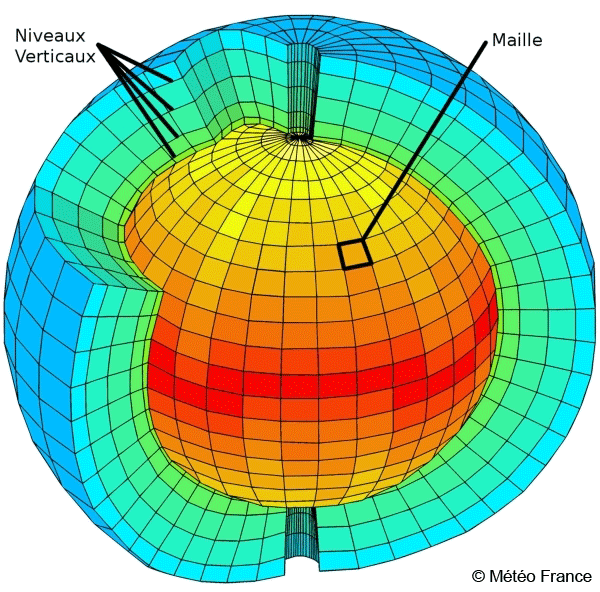
\includegraphics[width=4cm]{images/Chapitre1/maillage.png}
    \caption{\label{pic_maillage} Le maillage le plus fin exploité par Météo-France pour ses prévisions régionales restitue des mailles de 2,5 km de côté. (source \url{www.irma-grenoble.com})}
\end{figure}




\begin{enumerate}
\item Aéronautique: la Dynamique des Fluides (CFD) est utilisée pour valider qu'un flux d'air circule correctement autour des ailes pour essayer de maximiser le portage des ailes. 
\item Industries des hydrocarbures: la recherche pétrolière utilise le HPC pour analyser les fonds marins et modéliser les réservoirs de pétrole pour optimiser leur extraction.
\item Météorologie: pour améliorer les prédictions météorologiques mais aussi de les réaliser plus longtemps à l'avance. 
\item Sciences biologique: séquençage et alignement ADN, découverte de drogues 
\end{enumerate}



%%%%%%%%%%%%%%%%%%%%%%%%%%%%%%%%%%%%%%%%%%%%%%%%%%%%%%%%%%%%%%%
%%%%%%%%%%%%%%%%%%%%%%%%%%%%%%%%%%%%%%%%%%%%%%%%%%%%%%%%%%%%%%%
%%%%%%%%%%%%%%%%%%%%%%%%%%%%%%%%%%%%%%%%%%%%%%%%%%%%%%%%%%%%%%%
%%%%%%%%%%%%%%%%%%%%%%%%%%%%%%%%%%%%%%%%%%%%%%%%%%%%%%%%%%%%%%%

\subsection{Définition du Calcul Haute Performance}
 
 Le domaine du HPC est le domaine informatique qui consiste à regrouper des puissances de calculs pour qu'ensemble elles travaillent à la résolution d'un problème partagé. Comme expliqué dans la section précédente, la simulation numérique est utilisée dans des domaines très différents. Le point commun de ces applications est la résolution d'un gros problème qui ne peut pas être résolu par une seule ressource. Ce problème est divisé en sous-problème de petites tailles, qui eux peuvent être résolus séparément. Cette méthode de résolution est appelée le calcul parallèle, un exemple est donné dans la partie \ref{sub_reso_partage}. Aujourd'hui, les utilisateurs de HPC peuvent accéder à ces clusters par différents moyens:
\begin{enumerate}
\item \textbf{Dedicated supercomputer}, une architecture unique est créée. La conception de ces architectures étant unique, les frais de conception sont très élevés mais cette spécificité en fait des architectures très performantes car elles sont conçues spécialement pour répondre à un besoin précis. 
\item \textbf{Le Commodity cluster}, qui agrège du matériel grand public (haut de gamme) pour former des grappes de calculs de plusieurs milliers de processeurs.
\item \textbf{HPC as a service} ou HPC Cloud ou encore HPC dans le nuage,  utilise le modèle \textit{System as a Service} pour apporter aux entreprises manquant de moyens ou de compétences un accès à une infrastructure HPC externalisée. L'un des principaux avantages est la flexibilité d'usage (adapter l'infrastructure à son besoin). 
\item \textbf{Grid Computing} ou grille informatique est un regroupement de ressources informatique à grande échelle (nationale voir internationale). Par exemple \textit{Einstein@Home} \cite{PhysRevD.80.042003} est un projet de recherche mondial sur les ondes gravitationnelles  qui regroupe les ordinateurs de 50000 utilisateurs connectés à travers le monde qui sont utilisés pour  analyser les données transcrite par des capteurs.
\end{enumerate}


Quel que soit le moyen de conception et d'utilisation, ces architectures sont des regroupements de centaines, voire de milliers de ressources qui forment une grappe de serveur que l'on appelle un \textit{cluster} ou \textit{supercalculateur}. 

\subsubsection{Le marché du HPC}
Il y a plusieurs catégories d'acheteurs de cluster HPC qui n'ont pas tous les mêmes besoins et les mêmes budgets:
\begin{itemize}
    \item Le petit HPC: ce sont les clients avec les plus petits budgets comme par exemple des équipes d'ingénieurs ou des petites universités qui ont besoin d'un cluster de calcul pour des usages personnels. On pourra citer le projet SIMSEO qui à pour but de sensibiliser et d'accompagner les PME à utiliser la simulation numérique. Car même pour des entreprises de tailles réduite, la simulation et le HPC peuvent être des atouts clefs dans leur stratégie.
    \item Le HPC public: il regroupe les grandes universités qui partagent le matériel entre plusieurs écoles ou laboratoires de recherche. Ces systèmes sont d'une puissance élevée, et certains sont classé dans le \textit{TOP500}. Les codes exécutés sont souvent disponibles en open-source.
    \item Le HPC commercial: ce sont tous les clusters que les entreprises privées utilisent pour développer leur business. Les applications qui y sont exécutées sont souvent des applications privées.
\end{itemize}



%%%%%%%%%%%%%%%%%%%%%%%%%%%%%%%%%%%%%%%%%%%%%%%%%%%%%%%%%%%%%%%
%%%%%%%%%%%%%%%%%%%%%%%%%%%%%%%%%%%%%%%%%%%%%%%%%%%%%%%%%%%%%%%
%%%%%%%%%%%%%%%%%%%%%%%%%%%%%%%%%%%%%%%%%%%%%%%%%%%%%%%%%%%%%%%
%%%%%%%%%%%%%%%%%%%%%%%%%%%%%%%%%%%%%%%%%%%%%%%%%%%%%%%%%%%%%%%

\subsection{Les Clusters}
\begin{fancyquotes}
Un cluster (grappe) de serveurs est un \textbf{interconnexion} de \textbf{ressources informatiques} dans le but de \textbf{résoudre un problème} complexe de façon \textbf{partagée}. 
\end{fancyquotes}

A l'origine les premiers supercalculateurs étaient des architectures uniques crées de toutes pièces pour un client. Il était alors très dure de les reproduire ensuite rendant leur coût de conception très élevé. Seymour Cray présenta le premier super- calculateur en 1960 alors qu'il travaillait pour Control Data Corporation. A partir des années 1990 apparurent des clusters construits à partir de matériels haut de gamme mais qui peuvent s'acheter dans la grande distribution. Ce n'est donc pas la puissance individuelle de ces matériels qui est importe mais c'est le regroupement de centaines de stations de travail qui en fait des supercalculateur, et cette façon de les construire est toujours la même aujourd'hui.\\



%%%%%%%%%%%%%%%%%%%%%%%%%%%%%%%%%%%%%%%%%%%%%%%%%%%%%%%%%%%%%%%
%%%%%%%%%%%%%%%%%%%%%%%%%%%%%%%%%%%%%%%%%%%%%%%%%%%%%%%%%%%%%%%

\subsubsection{L'interconnexion } 
La liaison des serveurs se fait grâce au meilleurs technologies de réseaux pour atteindre le maximum de performances. Les caractéristiques principales de ces réseaux sont une latence faible et une bande passante élevée. Le terme de \textit{latence} fait référence au temps qu'il faut à un message (ou paquet de bits) pour aller d'un serveur à un autre. On utilise alors la milliseconde ou nano seconde comme unité. La bande passante quand à elle représente le nombre de messages qui peuvent être transporté en même temps entre deux serveurs, on utilise l'unité du gigaoctet. En simplifiant beaucoup; on peut voir le réseaux comme un tuyau, la vitesse de l'eau y circulant étant la latence, et son diamètre la bande passante. Et suivant le type d'application, la priorité n'est pas la même. On peut citer le domaine de la finance qui à besoin d'un réseaux extrêmement rapide pour exécuter des milliers d'opérations à la seconde. Alors qu'un hébergeur vidéo sera très sensible à la bande passante de son système pour pouvoir fournir du contenus à plusieurs clients.
Aussi, l'efficacité du réseau ne dépend pas seulement du matériel, la partie logiciel est tout aussi importante: des algorithmes de routages à la complexité des protocoles, tout est importants pour faciliter la livraisons des paquets de données. Enfin, la structures des switchs doit être bien pensée pour réduire le nombre de \textit{sauts} de chaque échanges, c'est à dire le nombre d'intermédiaire pour aller de l'expéditeur au destinataire. La figure \ref{pic_topologie} montre un exemple de topologie et l'impact qu'elle a sur la latence des communications qui peut être multiplié par deux suivant à qui la machine A s'adresse. Cette structure (ou topologie) doit s'assurer d'éviter tout risques de congestions afin qu'une partie de réseau ne soit pas trop sollicitée ce qui créerait des baisses de performances. 

\begin{figure}
    \center
    \includegraphics[width=4cm]{images/Chapitre1/TopologieReseau.png}
    \caption{\label{pic_topologie} Exemple d'une topologie d'un cluster. Si le serveur A veut envoyer un message à B, il devra effectuer 4 sauts (ou \textit{hop}).}
\end{figure}


%%%%%%%%%%%%%%%%%%%%%%%%%%%%%%%%%%%%%%%%%%%%%%%%%%%%%%%%%%%%%%%
%%%%%%%%%%%%%%%%%%%%%%%%%%%%%%%%%%%%%%%%%%%%%%%%%%%%%%%%%%%%%%%

\subsubsection{Les ressources informatiques} 
Les serveurs de calculs connectés grâce à ces réseaux ont aujourd'hui beaucoup de points communs et dépendent de moins en moins du vendeur qui les a conçus. Un cluster moderne est construit avec du \textit{commodity hardware}, du matériel produit en série. Que ce soit des processeurs à la mémoire, on peut trouver ces matériels sur le marché grand public. C'est seulement l'agglomération de ces serveurs par centaines, qui en fait des architectures unique et très puissante. Aujourd'hui la majorité des architectures systèmes est composée d'un serveur contenant un ou plusieurs processeurs qui est relié à sa mémoire, son disque et qui peut être accompagné d'accélérateurs comme des carte graphiques. Même si la majorité des architectures se ressemble cela ne les rend pas pour autant moins complexes car chaque composants cités précédemment est d'une complexité sans fin. Les mémoires par exemple compte des dizaines de technologies différentes avec chacune leur avantages et leurs inconvénients. De même que pour les processeurs qui sont au fil des années se sont complexifiés pour répondre à des besoins particuliers. L'élaboration d'un cluster doit donc prendre en compte tout ces aspects mais aussi les contraintes inhérente au projet (le prix, l'espace disponible ou la puissance électrique disponible). 

% ---------
\subsubsection{Résolution partagée}
L'interconnexion de toutes ces ressources est réalisée dans le seul but de réduire le temps nécessaire à la résolution d'un problème. En effet, pour une expérience donnée si l'on possède un cluster de 1000 machines on ne voudra pas réaliser l'expérience un millier de fois mais plutôt réduire le temps d'une expérience par un facteur 1000 pour ensuite analyser les résultats, changer les paramètres et pouvoir lancer une nouvelle expérimentation. La calcul parallèle est un ensemble de moyens, logiciel et matériel qui permettent de réaliser des instructions simultanément. L'idée principale du calcul parallèle est de réduire le temps de calcul d'un programme en divisant le travail à réaliser, le partager en sous-problèmes qui peuvent être résolu de façon indépendante par plusieurs ressources de calcul, comme des processeurs. Un exemple concret de résolution d'un problème grâce à la programmation parallèle est donnée dans la section \ref{sub_reso_partage}
\textbf{TODO fini cette section, une image}


% ---------


\subsubsection{Le TOP500 et le benchmark HPL}

\paragraph{Le benchmarking ou l'étalonnage} est une pratique courante qui consiste à évaluer plusieurs solutions en leur faisant passer un épreuve commune. Dans le domaine informatique cela permet de tester différentes architectures matériels et d'évaluer laquelle sera la plus performantes. Il existe plusieurs benchmark qui ont chacune leur particularités. Ces codes essayent de reproduire les opérations faites par des codes industriels, dans le but de faire des projections de performances et pouvoir comparer deux solutions. Le benchmark le plus populaire dans le domaine du HPC est celui développé par Jack Dongara en 1988: le benchmark HPL \cite{Dongarra}. C'est grâce à lui que le classement du TOP500 est réalisé deux fois par ans.


\paragraph{Le TOP500} \footnote{\url{www.top500.org}} est un classement mondial qui classe, tous les 6 mois depuis 1993, les 500 super-calculateurs les plus puissants au monde. Ce classement se base sur le nombre maximum d'opérations flottantes qui peuvent être exécutées en une secondes. Cette unité à été choisie car la grande majorité des codes utilisés dans les domaines précédemment cités, exécutent des opérations sur des nombres flottant. Il s'avère donc judicieux de choisir ce dénominateur commun pour comparer les différentes architectures.  Une opération flottante peut être traduite par \textit{floating point operation} ou FLOP en anglais, on parlera donc de FLOP/S ou FLOPS pour désigner le nombre d'opérations flottante par seconde. Pour réaliser ce benchmark tous les supercalculteurs doivent exécuter le même code, le benchmark LINPACK \cite{Dongarra} \cite{450b1baca0774fd0976ff739b90bed04}. Ce benchmark est un code simple qui résout un système d'équation linéaire de deux matrices $A$ et $B$ par $Ax = B$. L'avantage de ce code est que les performances évoluent linéairement avec le nombre de machines utilisées car il y a très peu de communication sur le réseaux. Le résultat est un nombre de FLOP/S que la machine peut exécuter, ce qui rend la comparaison avec d'autres supercalculateur facile. 



Le site web du \textit{top500} contient de nombreuses données. On peut par exemple voir la consommation électrique, le nombre de coeurs, ou encore si les clusters contiennent des cartes graphique. Sur le graphique \ref{pic_top500perf_evo}, on voit que la puissances des supercalculateurs augmente d'un facteur 1000 tous les 10 ans.
Il faut cependant savoir que ce classement ne contient pas toutes les machines. En effet, certains industriels ne préfèrent pas paraître dans ce classement. Stratégiquement parlant, il peut être intéressant de ne pas publier sa puissance de calcul et nous savons que les clusters les plus puissants n'y figurent pas. Cependant ce classement nous permet de voir les tendances que suivent la majorité des architectures pour comprendre comment elles évoluent.\\

\begin{figure}
    \center
    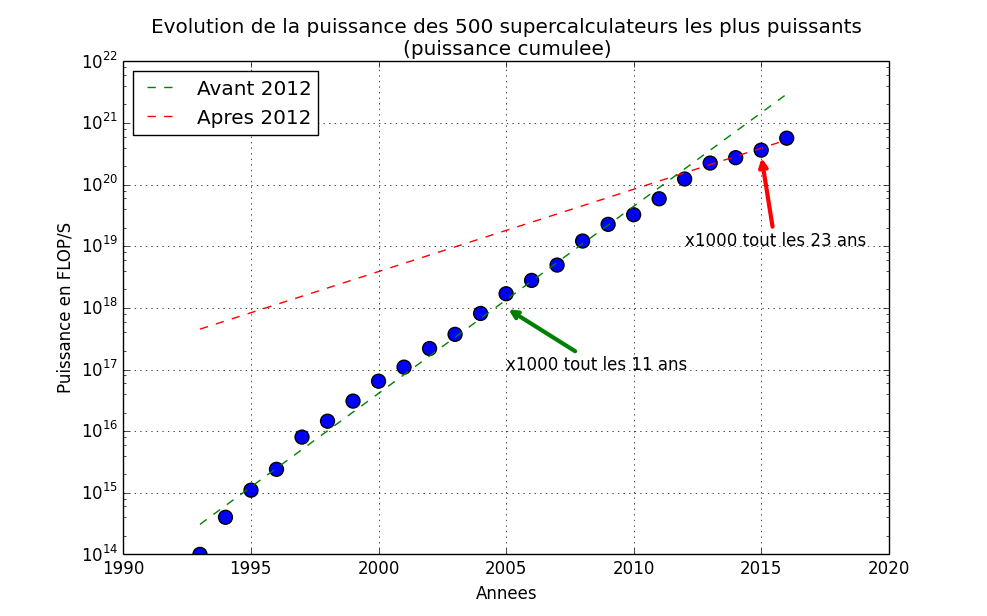
\includegraphics[width=10cm]{images/Chapitre1/pic_top500perf_evo.png}
    \caption{\label{pic_top500perf_evo} Évolution de la performance cumulée des 500 supercalculateurs les plus puissants au monde. La pente de l'évolution diminue à partir de 2012}
\end{figure}


Il existe un second classement qui classe les supercalculateur en fonction de leur ratio $\frac{FLOPS}{WATT}$ nommé le \textit{Green500} \cite{feng2007green500}. Comme nous allons le voir ensuite, la consommation électrique est devenus une contrainte forte dans l'architecture des nouveaux cluster. De plus en plus, la question n'est plus de construire le supercalculateur le plus puissant, mais le plus efficace.

\subsubsection{HPC ou HTC}
Aujourd'hui le domaine des supercalculateurs est souvent désigné par le terme HPC, mais il y a quelques précision à apporter quant à la mauvaise utilisation de ce terme. Il existe un autre domaine qui utilise les supercalculateur, le High Throughput Computing (HTC). En effet, la communauté à voulu donner un nom aux architectures capables d'exécuter différentes applications simultanément et ce sans interruptions sur plusieurs mois. Contrairement aux applications HPC qui exécutent des taches très dépendantes les unes des autres, les applications HTC se focalisent sur l'exécution des plusieurs tâches en parallèles et assure la disponibilité maximale du nombre de ressources dont dispose le supercalculateur. Prenons pour exemple un cluster de calcul partagé dans une université. L'objectif de cette machine n'est pas d'exécuter une application toute l'année, mais plutôt de répartir le matériel disponible entre les utilisateurs pour que tous puissent l'utiliser au maximum. Une majorité des clusters d'aujourd'hui fonctionnent sur le même modèle et l'utilisation de l'expression HPC pour les désigner est en fait un abus de langage.



% ------------------------------------



\section{Le domaine du HPC en 2017: challenges et contraintes}


\begin{fancyquotes}
Peu importe quelle puissance attendront les processeurs, le logiciel trouvera toujours une façon d'utiliser cette puissance. Construisez un processeur 10 fois plus rapide, et la partie logiciel trouvera toujours 10 fois plus à faire (ou le fera 10 fois moins efficacement)  \cite{sutter2005software}
\end{fancyquotes}


Dans cette section nous allons tout d'abord exposer quels sont les challenges du HPC en 2017, pourquoi nous en avons besoin plus que jamais. Dans une seconde partie nous aborderons les contraintes qui empêchent les super-calculateurs de continuer à augmenter leur puissance d'années en années comme cela se faisait jusqu'à maintenant.

\subsection{Les challenges et opportunités}

La création de cette collaboration entre l'école de l'ENS et HPE n'est pas due au hasard. Cette thèse a été créée alors que le domaine du HPC connais un ralentissement sans précèdent (graphique \ref{pic_top500perf_evo}. Depuis 2012 certaines barrières ont été atteintes et les processus qui permettaient aux architectures d'évoluer à cadence constante ne sont plus viables. 




\subsubsection{Exascale}
Aujourd'hui nous rencontrons des utilisations du HPC tous les jours, que ce soit quand nous regardons la télévision ou que nous consultons le cours de la bourse. Le HPC à un réel impacte sur nos vie, les rendant plus sécurisées en prévoyant précisément des catastrophes naturelles. tous les jours de nouvelles applications sont découvertes, et certaines ne sont techniquement pas envisagées car elles nécessiteraient trop de puissances de calculs. L'objectif de tous les constructeurs présent dans le domaine du HPC est la construction du premier ordinateur capable de réaliser  $10^18$ opérations sur des nombres rationnels par secondes, l'équivalent d'un \textit{exaflop} ($10^18$ Floating Point Operations). L'industrie s'est donc lancée dans cette course effrénée à l'exaflop. En effet, le premier constructeur qui y parviendra bénéficiera d'un grand coup marketing et acquerra de nombreux clients car la majorité des clients ont des problèmes ne pouvant être réglé que par un ordinateur de cette puissance, et attendent son arrivé.

\subsubsection{De nouveaux clients}
L'arrivée de l'exaflop va entrainer l'arrivée de nouveaux clients, et il est indispensable pour des constructeurs comme HPE d'être prêt à les accompagner. Avec l'apparition des objets connectés le monde connaît une explosion des données qui sont générées et collectées. Elles sont ensuite stockées dans des data centers, qui n'ont pas les puissances suffisantes pour pouvoir les analyser. En effet les données générées par les montres, les frigos connectés ou les capteurs dans des chaînes de productions n'ont pas réelle utilité si elles ne sont pas exploité grâce à des techniques de \textit{Data Mining}. Et l'arrivée du machine learning nous ouvre à un monde extraordinaire qui n'est possible que si nous créons les architectures adéquats pour en profiter. Un autre domaine nécessitant ces quantités de calculs est celui de la recherche médicale et biologique. Aujourd'hui nous sommes capables de simuler des réactions chimiques de quelques nano secondes et sur de petit volumes. La création de supercalculateur exaflopique serait une énorme avancée pour ces clients, et les constructeurs qui n'auront pas misé sur l'exascale seront terriblement impactés. Ces nouveaux clients sont une grosse opportunité pour une entreprise comme HPE. Une analyse de marché paru en 2016 montre que le marché du High Performance Computing pèsera 36 milliards de dollars en 2020, alors qu'il en valait 28 en 2015\footnote{\url{http://www.marketsandmarkets.com/Market-Reports/Quantum-High-Performance-Computing-Market-631.html}}. Cette augmentation de 5\% par année est due à l'explosion des quantités, à la complexité des techniques pour les analyser et les visualiser et de la demande grandissante de solution HPC dans de nombreux domaines.


\subsubsection{Les nouvelles technologies}
Dans l'objectif de construire des supercalculateur toujours plus puissant nous pouvons et allons pouvoir nous appuyer sur des évolutions technologiques majeures. En effet que ce soit au niveau des mémoires avec l'arrivée des mémoire non-volatile (NVM memory), ou au niveau des réseaux avec la photonics. Il va falloir que, constructeur comme client, se tienne à jour de toutes ces évolutions technologique qui vont modifier les façon de programmer et de construire les architectures. HPE à un un projet de machine exascale nommé The Machine. Cette architecture très novatrice s'appuie sur trois piliers technologiques: les mémoires \textit{memristors} et les réseaux à base de fibre: la \textit{ photonic}. La troisième avancée et la restructuration complète de l'architecture d'un super calculateur grâce au protocole de communication Gen-Z.\\

%*****************************************************************************************************

\subsection{Les contraintes}
La loi de Moore prevoyait une augmentation exponetielle de la puissance des processeurs, mais une telle augmentation ne peut pas continuer indéfiniment car nous avons atteints certaines limites physiques. La course à l'exascale est lancée mais il existe beaucoup de contraintes qui ralentissent et compliquent ce challenge technologiques. Les contraintes sont multiples et n'influe pas autant sur les performances, mais depuis 2012 on assiste à un changement de dynamique (voir le graphique \ref{pic_top500perf_evo}). Cette partie liste donc les contraintes majeures qui impactent le domaine du calcul haute performance.


\subsubsection{Électrique}
L'électricité est une forte contrainte dans l'élaboration de ces clusters et elle est un facteur majeur du ralentissement de l'évolution des performances des super-calculateur du TOP500 vu sur la figure \ref{pic_top500perf_evo}. En effet, aujourd'hui les puissances électriques nécessaires pour alimenter ces machines dépasse la capacité des lignes électriques qui arrivent jusqu'aux centre de calculs. Notre stratégie d'augmenter le nombre de serveurs pour augmenter la puissance totale n'est plus valable. Ce problème n'est pas nouveau et de nombreux efforts ont déjà était fait sur les alimentations et le refroidissement qui sont proche de l'idéal. Nous avons tendance à penser que l'investissement dans un super-calculateur est réaliser lors de son achat, mais un budget conséquent doit être alloué pour son alimentation. En simplifiant, on peut ramener le prix de l'électricité à 1 dollar par watt durant une année. Si on regarde la consommation électrique des clusters du Top500, on constate qu'en moyenne ils consomment 1.4 mégawatt et que les 5 qui consomment le plus sont au dela de 12 mégawatt (voir graphique \ref{pic_top500_power}). Facilement on calcul que l'alimentation de ces architectures coûte des millions de dollars chaque années (20 millions de dollars pour le premier).
L'objectif est donc d'augmenter le nombre de calcul que l'on réalise pour une puissance électrique donnée, c'est à dire augmenter le ratio $\frac{FLOP}{Watt}$. PathForward à récemment publié les exigences technique auxquelles supercalculateur exascale allé devoir répondre \cite{PathForward_Req}. Cette étude montre qu'un système exascale ne devra consommer entre 20 et 30 megawatt. Ce qui n'est pas si loin de la consommation des deux clusters les plus puissant (19 et 18 mégawatt). D'autant plus si on compare au saut de performances que l'on doit faire pour atteindre l'exaflop. Il va falloir avec 50\% d'énergie en plus, réaliser 30 fois plus d'opérations. L'écart entre ces deux facteurs va nous obliger à repenser à comment les codes sont exécutés et dans un second temps de repenser entièrement les architectures.


\begin{figure}
    \center
    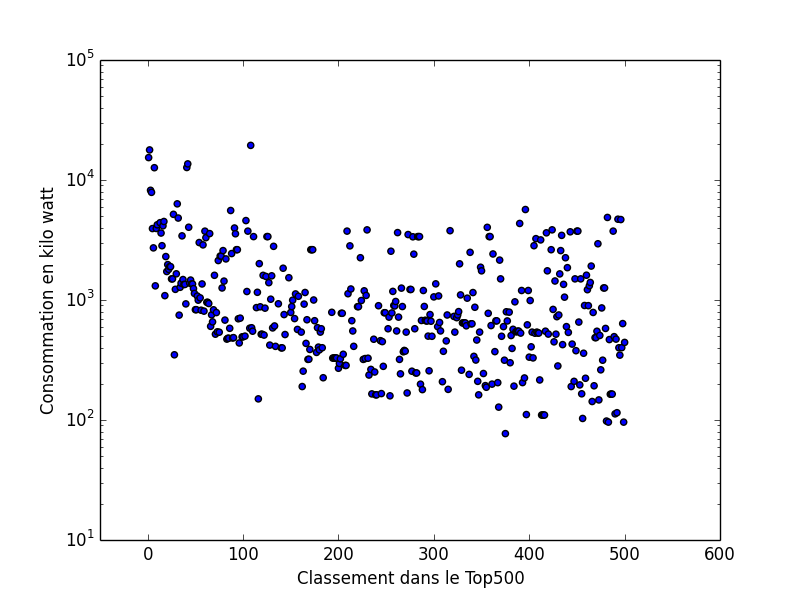
\includegraphics[width=10cm]{images/Chapitre1/pic_top500_power.png}
    \caption{\label{pic_top500_power} Consommation électrique des 500 supercalculateurs les plus puissants.}
\end{figure}



\subsubsection{Économique}
Le domaine du HPC est fortement influé par l'économie. En effet la construction de ces infrastructures coûte des millions d'euros d'investissement, et du fait que ces super-calculateurs sont des piliers stratégiques des entreprises, ces dernières sont très regardantes à leur coût. Cette forte pression de l'économie est une contrainte et il est difficile de proposer des sauts technologiques qui nécessitent de lourd investissement en amont sans connaître les retombés à l'avance. Comme vu dans la section consacré à l'énergie, nous devons repenser la façon dont nos codes sont conçus et exécutés. Par exemple en allant vers de nouvelles architectures comme les FPGA (Field Programmable Gate Array). Cette technologie permet de faire des périphériques très efficace en terme de consommation électriques. L'idée principale étant de laisser au programmeur le développement complet du circuit électronique pour qu'il corresponde parfaitement à son besoin. Mais la programmation de tels circuits est très complexe et demande des mois, souvent des années pour les codes complexes, pour être réalisée. Ainsi, malgré l'efficacité, prouvée, de cette technologie, les entreprises ne s'y lance pas à cause des coûts engendrés par les taille des équipes requises pour les programmer dans un temps raisonnable. On voit donc qu'il n'y a pas que les avancées et les nouvelles technologie qui sont importantes, il y a aussi leur facilité d'accès

\subsubsection{Technologiques}
Les différentes technologies connaissent elles aussi plusieurs contraintes. Une des principale à été exposé par Gordon Moore en 1965 qui a réalisé une conjecture qui est devenue la loi éponyme connus de tous. La loi de Moore prévoit que l'évolution du nombre de transistors sur une surface donnée va, grâce aux évolution technologique, être doublée tous les 2 ans à un prix constant. Sur la figure \ref{pic_Moore_prediction} on voit bien que cette évolution sur bel et bien la conjecture que le co-fondateur d'Intel a fait il y a plus de 50 ans.

\begin{figure}
    \center
    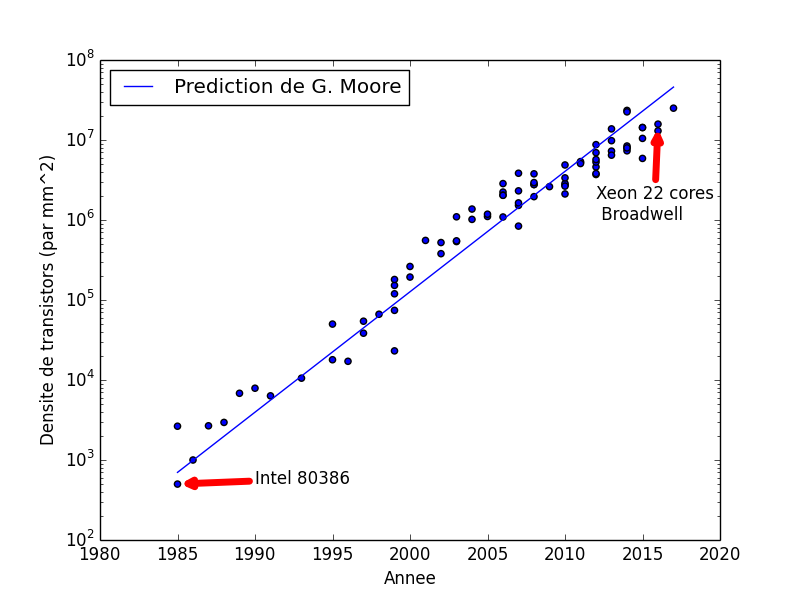
\includegraphics[width=10cm]{images/Chapitre1/Moore_prediction.png}
    \caption{\label{pic_Moore_prediction} La loi de Moore décrit l'évolution de la densité de transistors qui double tous les deux ans pour un prix constant (Données:  \url{https://en.wikipedia.org/wiki/Transistor_count}).}
\end{figure}


\textbf{TODO $Seminar_intro_v5.pdf$ slide 9 - expliquer moore par deux graphique: prix par mm2 et finesse de gravure}
Comme la puissance de calcul des processeurs est directement liée au nombre de transistors qu'ils contiennent, la puissance des puces à elle aussi suivi cette cadence. Alors pourquoi est ce devenu une contrainte ? Parce que pour doubler le nombre de transistors sans changer la surface gravée, il faut graver des transistors deux fois plus petits. Et si depuis 1965 on parvenait à le faire  au prix de nombreuses avancée techniques des appareils de gravure, nous atteignons aujourd'hui une limite physique, celle de la taille des atomes, voir figure \ref{pic_Moore_gravure}. En effet, aujourd'hui nous parvenons à graver des puces en autour de 10nm,  l'équivalent de quelques atomes. A cette taille les courants électriques ne sont plus stables et la course à la réduction des finesses de gravure est terminée. Alors qu'elle était un vecteur essentiel de l'évolution des performances, il va nous falloir trouver d'autres moyens pour arriver à atteindre l'exascale.

\textbf{TODO $Seminar_advanced technologies_v5.pdf$ slide 93 limite de Landauer}

\begin{figure}
    \center
    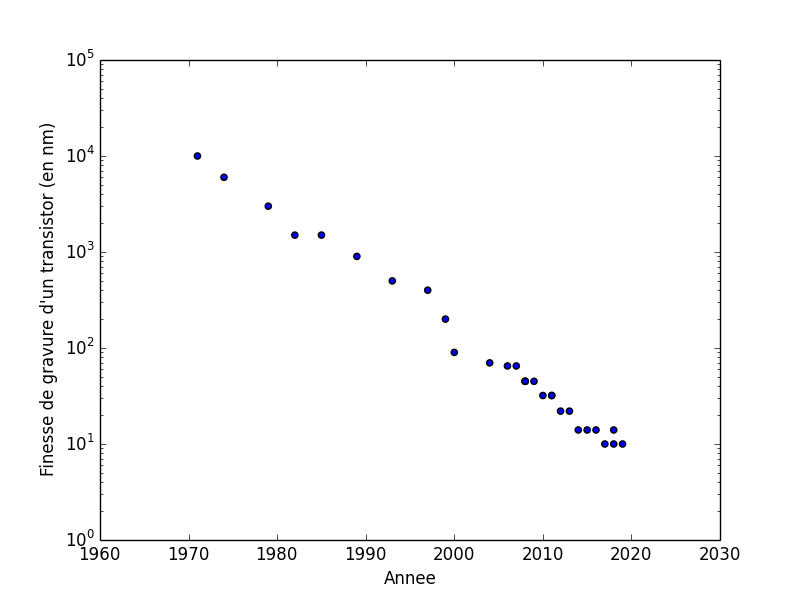
\includegraphics[width=10cm]{images/Chapitre1/Moore_gravure.png}
    \caption{\label{pic_Moore_gravure} La finesse des gravures à largement diminuée mais elle commence à toucher les limites de la physique \url{https://fr.wikipedia.org/wiki/Microprocesseur}).}
\end{figure}

La contrainte technique est très forte, d'autant plus avec l'apparition de nouvelles technologies plusieurs fois par ans. D'autant plus que souvent, ces nouveautés ne sont pas simplement des versions améliorées de précédents produits, ce sont souvent des technologies innovantes. Par exemple en c'est à partir de 2010 que l'on voit les premiers clusters contenant des cartes graphiques. Et il a fallut plusieurs années pour que cette technologie se fasse une place dans le monde du HPC notamment parce qu'elle nécessite une complète réécriture des codes. Il faut repenser la structure des algorithmes pour pouvoir tirer partie de tout le potentiel de ces cartes. Et il faut attendre 2013 pour voir une réelle percée de cette technologie (voir le graphique \ref{pic_GPU_repartition_TOP500}). Et il en est de même pour de nombreuses technologies innovantes, l'arrivée des mémoires non volatiles va demander aux utilisateurs de repenser une nouvelle fois leur algorithmes et seules des programmeurs expérimentés et avisés pourront le faire. L'exemple du FPGA est aussi un très bon exemple, sa complexité de programmation est un gros frein à son adoption. Et ces contraintes techniques se traduisent directement par un coût pour les entreprises. Car il faut engager des experts des différents domaines et investir de nombreuses heures pour faire les transformations adéquates.     


\begin{figure}
    \center
    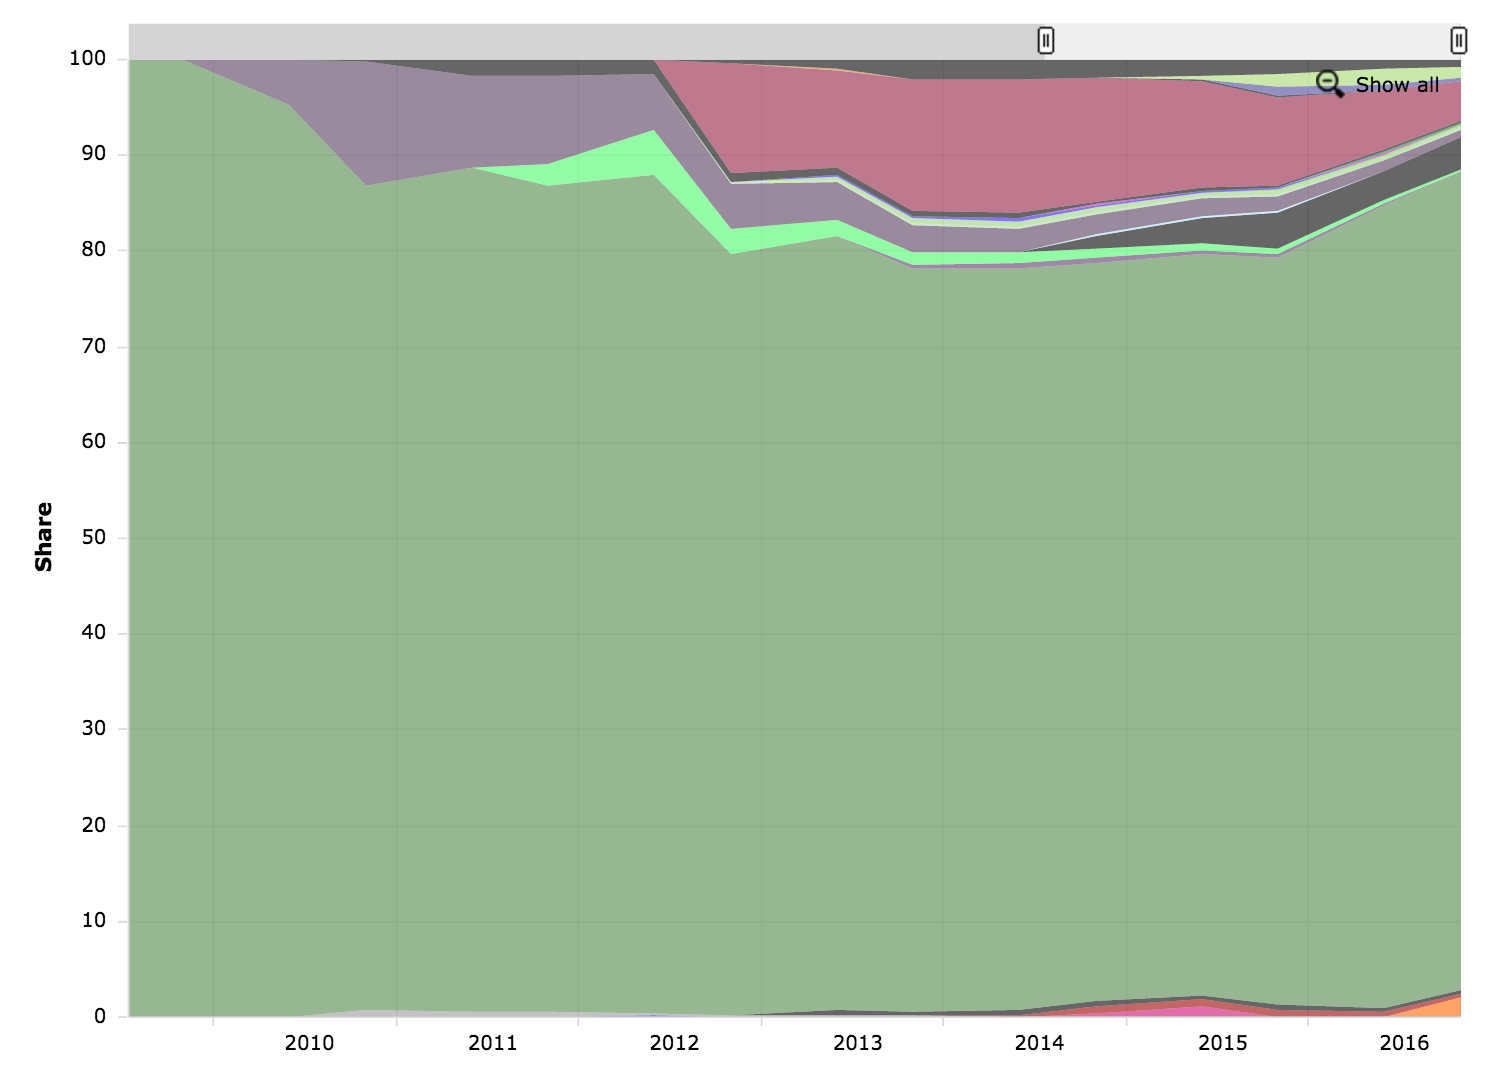
\includegraphics[width=10cm]{images/Chapitre1/pic_GPU_repartition_TOP500.png}
    \caption{\label{pic_GPU_repartition_TOP500} Partage de la performance totale du TOP500 entre les processeurs (couleur verte dominante) et les cartes graphiques (autres couleurs, représentants chaque modèles de cartes) \textit{source: \url{www.top500.org}}  }
\end{figure}

\subsubsection{Techniques et Connaissances}


Mes 3 ans d'expériences chez HPE et mon semestre de cours à Barcelone m'ont appris une chose: le domaine de l'analyse et des optimisations de performances est très difficile et nécessite de nombreuses connaissances et beaucoup d'expérience. La complexité des  architectures est telle qu'il est devenu impossible de prévoir avec précision leur comportement. Et ceci pour deux raisons: la première est le manque de connaissances fines de ces architectures et la deuxième est la faiblesse et la rareté des outils disponibles pour pour réaliser ce travail. En effet, pour contre balancer la complexité grandissante des architectures, il faut pouvoir utiliser des outils qui permettent de la comprendre. Or, la pauvreté des outils disponibles se fait ressentir et ceci pour une raison: personne n'en avait une réelle utilité jusqu'à maintenant. En réalité, il n'était pas nécessaire aux programmeurs de comprendre en détails toutes les finesses et toutes les particularités des architectures pour atteindre les performances voulues. Jusqu'à aujourd'hui il a suffit à l'industrie d'attendre les nouvelles versions des processeurs Intel (fameux modèle \textit{tic toc}) pour augmenter leur performances. Le travail d'optimisations ne valait alors pas le coup. C'est ainsi qu'aujourd'hui, alors que les contraintes se font plus pressantes que jamais, le domaine du HPC accuse le manques de développement d'outils et de formation de programmeur capable d'aller chercher ces performances.

De plus, les supercalculateurs se veulent de toujours plus hétérogènes en accueillant des accélérateurs diverses. Il faut donc calibrer les codes pour pouvoir être exécutés sur ces différentes architectures. Généralement, il faudra choisir un premier modèle de programmation dit à "mémoire distribuée". Il correspond à la partie du code qui s'occupe de partager le problème à résoudre entre les serveurs et qui s'occupe des communications. Le standard le plus utilisé celui de MPI (Message Passing Interface). Une fois le problème partagé, il faut coder le programme qui s'exécutera sur chaque serveurs, qui peuvent contenir plusieurs processeur. On utilise pour cela un deuxième paradigme de programmation, celui dit de "mémoire partagée". Enfin, ces serveurs peuvent aussi utilisé des accélérateurs (GPU, FPGA, DSP, etc.), il faudra donc écrire les programmes qui leur correspondent pour pouvoir les utiliser.
Les outils capables de nous aider dans ce travail nous manques et il est un objectif de cette thèse de fournir de tels outils. Mais il faut aussi user d'une méthodologie précise pour comprendre et optimiser ces codes. Fournir seulement un éventails d'outils ne sera pas suffisant si nous ne prodiguons pas les conseils que seule l'expérience peut apporter. Il est primordial de comprendre comment les codes sont exécutés sur nos système pour pouvoir espérer cibler de futures architectures comme \textit{The Machine}.



%%%%%%%%%%%%%%%%%%%%%%%%%%%%%%%%%%%%%%%%%%%%%%%%%%%%%%%%%%%%%%%%%%%%
%%%%%%%%%%%%%%%%%%%%%%%%%%%%%%%%%%%%%%%%%%%%%%%%%%%%%%%%%%%%%%%%%%%%
%%%%%%%%%%%%%%%%%%%%%%%%%%%%%%%%%%%%%%%%%%%%%%%%%%%%%%%%%%%%%%%%%%%%
%%%%%%%%%%%%%%%%%%%%%%%%%%%%%%%%%%%%%%%%%%%%%%%%%%%%%%%%%%%%%%%%%%%%
%%%%%%%%%%%%%%%%%%%%%%%%%%%%%%%%%%%%%%%%%%%%%%%%%%%%%%%%%%%%%%%%%%%%
%%%%%%%%%%%%%%%%%%%%%%%%%%%%%%%%%%%%%%%%%%%%%%%%%%%%%%%%%%%%%%%%%%%%
%%%%%%%%%%%%%%%%%%%%%%%%%%%%%%%%%%%%%%%%%%%%%%%%%%%%%%%%%%%%%%%%%%%%
%%%%%%%%%%%%%%%%%%%%%%%%%%%%%%%%%%%%%%%%%%%%%%%%%%%%%%%%%%%%%%%%%%%%
%%%%%%%%%%%%%%%%%%%%%%%%%%%%%%%%%%%%%%%%%%%%%%%%%%%%%%%%%%%%%%%%%%%%
%%%%%%%%%%%%%%%%%%%%%%%%%%%%%%%%%%%%%%%%%%%%%%%%%%%%%%%%%%%%%%%%%%%%
%%%%%%%%%%%%%%%%%%%%%%%%%%%%%%%%%%%%%%%%%%%%%%%%%%%%%%%%%%%%%%%%%%%%
%%%%%%%%%%%%%%%%%%%%%%%%%%%%%%%%%%%%%%%%%%%%%%%%%%%%%%%%%%%%%%%%%%%%
%%%%%%%%%%%%%%%%%%%%%%%%%%%%%%%%%%%%%%%%%%%%%%%%%%%%%%%%%%%%%%%%%%%%
%%%%%%%%%%%%%%%%%%%%%%%%%%%%%%%%%%%%%%%%%%%%%%%%%%%%%%%%%%%%%%%%%%%%
%%%%%%%%%%%%%%%%%%%%%%%%%%%%%%%%%%%%%%%%%%%%%%%%%%%%%%%%%%%%%%%%%%%%
%%%%%%%%%%%%%%%%%%%%%%%%%%%%%%%%%%%%%%%%%%%%%%%%%%%%%%%%%%%%%%%%%%%%
%%%%%%%%%%%%%%%%%%%%%%%%%%%%%%%%%%%%%%%%%%%%%%%%%%%%%%%%%%%%%%%%%%%%
%%%%%%%%%%%%%%%%%%%%%%%%%%%%%%%%%%%%%%%%%%%%%%%%%%%%%%%%%%%%%%%%%%%%

\section{Évolution des processeurs}

L'objectif de cette partie est de comprendre comment les architectures d'aujourd'hui sont devenues si complexes. Pour cela, nous allons étudier les évolutions technologiques chronologiquement pour comprendre en quoi elles étaient nécessaires et à quelle problématique elles répondent. Cet historique des ordinateurs bien que très complet n'aborde pas tous les points de ces architectures, mais seulement celles qu'il est important d'étudier pour comprendre l'état actuel de l'industrie.




%%%%%%%%%%%%%%%%%%%%%%%%%%%%%%%%%%%%%%%%%%%%%%%%%%%%%%%%%%%%%%%%%%%%
%%%%%%%%%%%%%%%%%%%%%%%%%%%%%%%%%%%%%%%%%%%%%%%%%%%%%%%%%%%%%%%%%%%%
\subsection{L'architecture}
Pour résoudre la multitudes de problèmes auxquels nous voulons apporté des réponses, nous utilisons des algorithmes. Pour écrire ces algorithmes on utilise des langages de programmation compréhensibles par un humain. Ces programmes sont alors lus par un programme appelé compilateur qui s'occupe de transformer le langage en un code compris seulement par le processeur qui lui pourra exécuter ces instructions. L'architecture de ces processeurs à beaucoup évolué depuis leur création, mais l'organisation globale n'a pas changé: la majorité des processeurs sont basés sur l'architecture \textit{Von Neumann}. C'est en 1945 que cette architecture à été présenté pour la première fois par John von Neumann dans un papier qu'il n'aura pas le temps de finir "First Draft of a Report on the EDVAC". Il y décrit une façon d'organiser un système électronique dans le but d'exécuter des instructions. La principale idée de cette architecture est la présence de 4 modules principaux:
 \begin{itemize}
    \item Une unité de traitement (CPU) qui contient une unité arithmétique et logique (ALU) qui s'occupe d'exécuter les opérations de bases (addition, multiplication, etc.) ainsi que de registres pour mémoriser les données utilisés pour leur exécutions
    \item L'unité de control qui lit les instructions et organise leur instructions en s'occupant de demander les données nécessaires à la mémoire.
    \item Une mémoire qui contient toutes les données nécessaires à l'éxécution du code mais aussi le code à éxecuter.
 \end{itemize}
 

 
 Dans ce papier il est précisé que la façon dont sont stocké le code à exécuter et les données en mémoires doit être la même contrairement à sa principale concurrentes, l'architecture  Harvard (figure \ref{pic_neumannHarvard}). Dans cette dernière, les instructions et les données sont stockées dans deux mémoires différentes et sont accédées par deux bus. Elles peuvent donc être accédées simultanément. Le problème de cette architecture vient des compilateurs qui souvent écrivent les données directement dans les instructions et les séparés n'a alors aucun interet. Aussi, la mémoire des instructions n'est accessible qu'en lecture rendant empêchant le programme de se modifier lui même ce qui est courant dans les codes (notamment du noyeau linux). Enfin la nécessité d'avoir deux bus rend les puces Harvard plus cher et les performances sont souvent moins bonnes. Un code qui aurait beaucoup d'accès mémoire ne pourrait pas profiter de la disponibilité du canal allant à la mémoire des instructions. Dans une architecture Von Neumann à deux canaux, les bus peuvent être utilisés aussi bien pour des instructions que pour les données.
 

\begin{figure}
    \center
    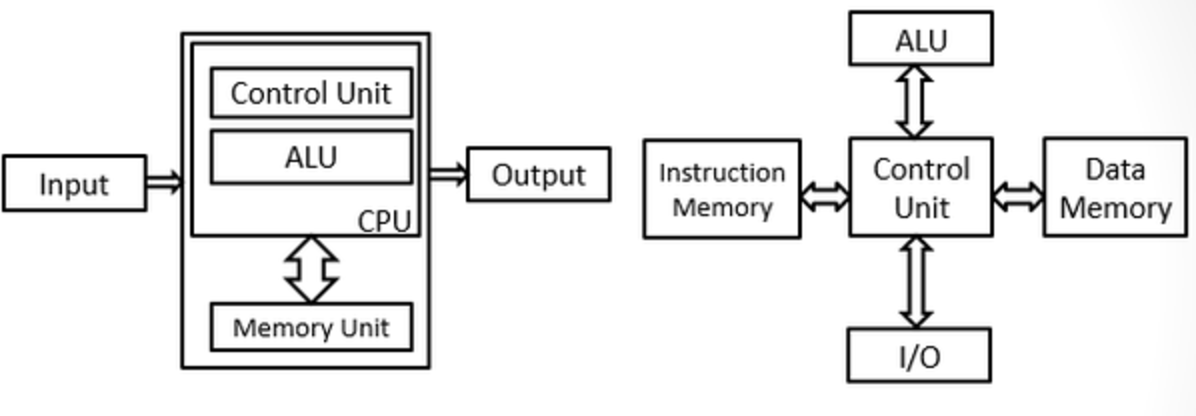
\includegraphics[width=10cm]{images/Chapitre1/neumannHarvard.png}
    \caption{\label{pic_neumannHarvard} Les deux principales architectures de processeurs: Von Neumann et Harvard. }
\end{figure}

Les architectures modernes des processeurs sont toujours construites sur ce modèle même si beaucoup de composants ont été ajoutés autour. L'architecture Von Neumann n'est capables de réaliser des calculs seulement avec les données présentes dans sa mémoire interne, les registres. Ainsi il faut charger les données présentes en mémoire jusque dans ces registres pour pouvoir effectuer les opérations. Et un problème majeur de cette architecture vient nous impacter très fortement 40 ans après sa création. En séparant ainsi la parti de calcul et la mémoire, le temps d'exécution d'un code est devenu très dépendant des liens qui relient ces deux parties. Ainsi, suite à de nombreuses avancés technologiques, les processeurs calcul 1000 fois plus vite qu'il ne faut de temps pour charger les données depuis la mémoire au processeur. Et les accès à la mémoire sont très fréquents comme on le voit sur la figure \ref{pic_Neumann}. Il faut charger les instructions à exécuter, charger les données nécessaires au calcul et enfin enregistrer le résultat. Ces liens sont donc très utilisés et sont devenus le  principal goulot d'étranglement, ou \textit{bottleneck} des applications. 



%%%%%%%%%%%%%%%%%%%%%%%%%%%%%%%%%%%%%%%%%%%%%%%%%%%%%%%%%%%%%%%%%%%%
%%%%%%%%%%%%%%%%%%%%%%%%%%%%%%%%%%%%%%%%%%%%%%%%%%%%%%%%%%%%%%%%%%%%
\subsection{Les instructions}
Un processeur exécute des instructions qui analysées par l'unité de traitement. Ces instructions sont en quelque sorte des mots appartenant à un langage que le processeur sait reconnaître. Pour que les programmes soient exécutables sur différentes architectures, il a fallu se mettre d'accord sur un langage à adopter, on appelle cela une ISA pour \textit{instruction set architecture}. Il existe deux familles d'ISA les jeux d'instrucions CICS pour \textit{Complex Instruction Set Computing} et les instructions RISC pour \textit{Reduced Instruction Set Computing}.

\subsubsection{CISC}  est la première famille d'instructions à avoir été utilisé massivement. Ces instructions sont dites complexes car une seule instructions peut à elle seule demander plusieurs opérations à réaliser. Par exemple une addition CISC s'occuperait de charger les données à la mémoire et d'exécuter l'addition ensuite. A l'origine beaucoup de codes étaient écrit en assembleur, et ce genre d'instructions permettaient au programmeur d'éviter d'écrire de nombreuses lignes de codes souvent redondantes. De plus les codes générés en CISC sont plus petit et nécessitent donc moins de mémoire, qui à l'origine manquait énormément.

\subsubsection{RISC} Le terme \textit{réduit} fait réference au nombre d'instructions plus petit que celles de CISC mais aussi pour signifier que le travail à réaliser par une instructions était moindre que pour une instruction CISC. En effet les instructions RISC sont exécutés en un seul cycles et correspondent à toutes les opération basiques que peut faire processeur. Pour réaliser une multiplications entre deux données, on devra alors explicitement charger la première donnée, puis la deuxième et enfin écrire l'instruction qui correspond à ma multiplication. Les instructions étant plus nombreuses le travail des compilateurs est augmenté mais souvent l'exécution des codes résultantes en est réduite. Les architectures nécessitent moins de transistors ce qui peut permettre d'augmenter le nombre de registres par exemple.

 Le RISC fut une réponse apporté a la lenteur de décodage du CISC et en 1970 John Cocke alors ingénieur chez IBM proposa de réduire le nombre d'instructions CISC et alors ont commencé à apparaitre des architectures RISC. En effet avoir des instructions complexes, même si rarement utilisées, augmente aussi la complexité de l'électronique utilisée pour les décoder. La philosophie du RISC est d'être rapide pour les cas communs d'utilisation et d'être le plus simple possible. Ces deux familles d'instructions ont toutes deux leurs avantages et leurs inconvénients et les puces actuelles comportent des parties qui executes du code en RISC et d'autres en CISC. L'ISA la plus rependu est le x86 qui se veut être un jeu d'instruction CISC. Le RISC augmente le nombre d'instructions lues séparément par le micro-processeur, si cela à le désavantage de consommer plus de mémoire, cela à aussi d'autre avantages, comme de pouvoir optimiser leur exécution avec la mise en place d'un \textit{pipeline}.
 
 \subsubsection{Le jeu d'instructions d'Intel: le x86} \textbf{TODO}
 
 
%%%%%%%%%%%%%%%%%%%%%%%%%%%%%%%%%%%%%%%%%%%%%%%%%%%%%%%%%%%%%%%%%%%%
%%%%%%%%%%%%%%%%%%%%%%%%%%%%%%%%%%%%%%%%%%%%%%%%%%%%%%%%%%%%%%%%%%%%
\subsection{Le pipeline } 
\label{sub_pipeline}
La chaîne de traitement du processeur, ou \textit{pipeline}, est une implémentation matériel d'un module qui permet de découper l'exécution d'une instructions en plusieurs étapes. Cette technique à pour effet de réduire drastiquement le nombre de cycles nécessaires à l'exécution d'un code. Le fait de partager l'exécution d'une instruction en sous étapes permet de commencer l'exécution de la suivante pendant que l'instruction actuelle est encore dans la chaîne d'exécution (voir figure ~\ref{pic_pipeline}).
\begin{figure}
    \center
    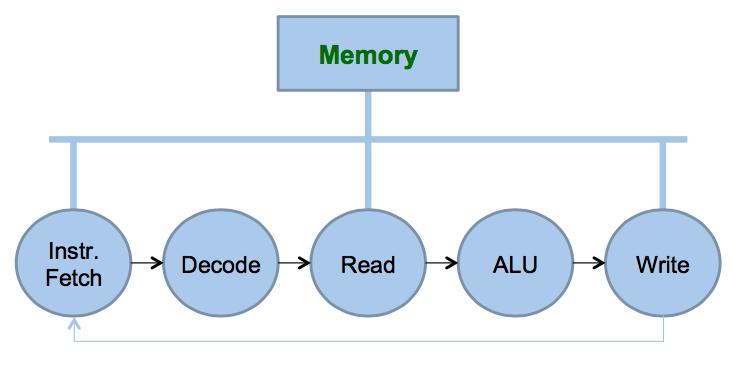
\includegraphics[width=10cm]{images/Chapitre1/Neumann.png}
    \caption{\label{pic_Neumann} Représentation simplifié d'un pipeline de 5 étapes.}
\end{figure}

 Il est commun de présenter la notion de pipeline avec un pipeline de 5 niveaux:

\begin{itemize}
    \item \textbf{Recherche de l'instruction} ou \textit{fetch}: cette première étape charge l'instruction à exécuter depuis la mémoire principale dans un registre du processeur. Grâce à un compteur interne, le registre \textit{Program Counter}, le processeur connaît l'adresse mémoire de la prochaine instruction à charger.
    \item \textbf{Décodage} ou \textit{décode}: une fois que l'instructions est chargé il faut la décoder pour déterminer quelle action il doit exécuter et quelles données sont nécessaires.
    \item \textbf{Execution} ou \textit{execute}: c'est durant cette étape que l'instruction est réellement exécuté. Suite au décodage le processeur peut réaliser plusieurs actions: utiliser l'ALU pour faire une opération, réaliser des mouvements de données ou déplacer l'exécution à une nouvelle adresse (branchement conditionnel ou \textit{branch})
    \item \textbf{Accès mémoire} ou \textit{memory}: lorsqu'une instructions est un acces mémoire (\textit{load} ou \textit{store}), c'est durant cet étape qu'il est réalisé.
    \item \textbf{Ecriture du résultat} ou \textit{write back}: Enfin le processeur doit enregistrer le résultat produit par l'étape \textit{execute}. Si c'est un branchement, il modifie le registre PC, si c'est une opération arithmétique il sauvegarde le résultat dans l'adresse destinataire.
\end{itemize}

On peut par exemple commencer à charger la prochaine instruction (étape \textit{fetch}), alors que l'instruction actuelle est en train d'être exécutée (étape \textit{execute}). Sur la figure \ref{pic_pip_yes} on assiste à l'exécution de 5 instructions, au premier temps un seul instruction est exécutée, à l'étape $IF$ pour \textit{instruction fetch}. Ensuite (ligne suivante) une nouvelle instruction est chargé (opération $IF$) pendant que la première est passé à l'étape suivante (opération $ID$). Ainsi au bout de 5 cycles, chaque étape du pipeline est utilisée (partie en verte). 



\begin{figure}[t!]
    \begin{subfigure}[t]{0.5\textwidth}
        \centering
        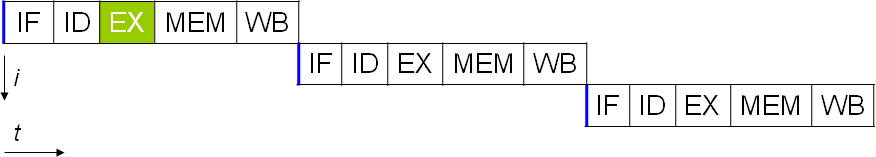
\includegraphics[height=0.4in]{images/Chapitre1/pipelineNo.png}
        \label{pic_pip_no}
        \caption{Processeur sans pipeline}
    \end{subfigure}%
    \begin{subfigure}[t]{0.5\textwidth}
        \centering
        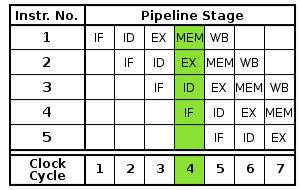
\includegraphics[height=0.7in]{images/Chapitre1/pipelineYes.png}
        \caption{Processeur avec un pipeline à 5 étages}
        \label{pic_pip_yes}
    \end{subfigure}
    
    \caption{Pipeline: en séquençant les instructions le processeur est capable d'exécuter des étapes différentes en parallèles (\textit{IF: instruction fetch, ID: instruction decode, EX: execution, MEM: memory, WB: write back}). Le nombre de cycle necessaire pour l'exécution passe alors de 25 à 9 cycles pour exécuter 5 instructions (source: \url{https://fr.wikipedia.org/wiki/Pipeline_(architecture_des_processeurs)} }
    \label{pic_pipeline}
\end{figure}





En 1939 IBM conçoit le premier processeur avec pipeline. Ce n'est qu'en 1989 qu'Intel produira le siens. Le nombre d'étapes, ou profondeur du pipeline, était de 2 à l'origine et a augmenté au fil du temps atteignant 31 étapes pour l'architecture du Pentium 4 Prescott d'Intel en 2004. Mais l'agrandissement du pipeline n'est pas gratuite, en effet, une chaîne de traitement plus grande prendra plus de place sur la puces et consommera plus d'énergie. Sur la figure \ref{pic_pipeline_evo} on voit que la consommation électrique a freiné l'évolution de la taille du pipeline.


 \begin{figure}
    \center
    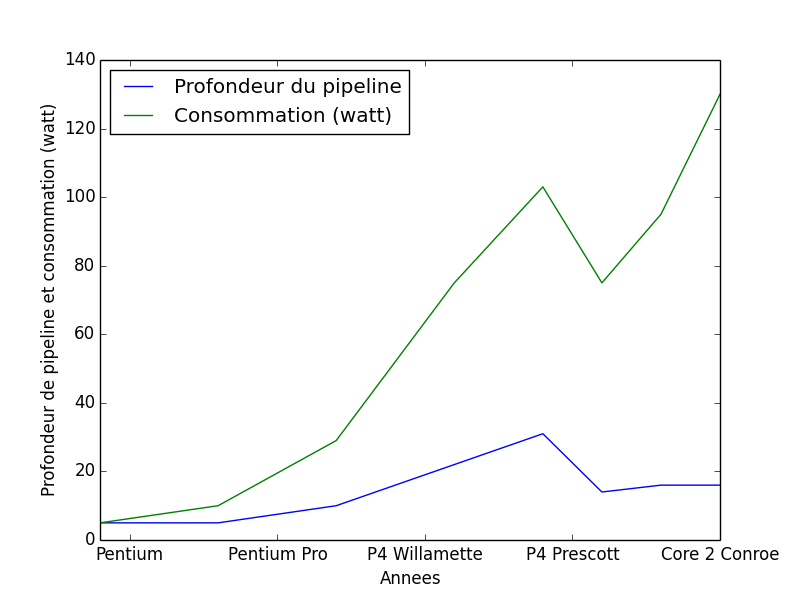
\includegraphics[width=7cm]{images/Chapitre1/pipeline_evo.png}
    \caption{\label{pic_pipeline_evo} L'évolution de la taille du pipeline des processeurs influe sur la consommation électrique}
\end{figure}

L'implémentation du pipeline à aussi ouvert la porte a de nombreuse optimisations. Ici sont présentés les avancées majoritaires qui vont impacter notre stratégie d'optimisation des codes.

\subsubsection{Pré-extraction - prefetch}

\begin{fancyquotes}
La pré-extraction est une technique efficace d'accès aux donnés qui permet de masquer l'attente du processeur quand une donné lui manque et pour diminuer la différence de performance entre les processeur et les mémoires. \cite{Byna2009}
\end{fancyquotes}

Un des défis des processeur est de réduire au maximum l'attente de donnés en provenances de la mémoire. Après avoir chargé la donné le processeur la décode, s'il a besoin d'une donnée pour réaliser un calcul par exemple il la demande à la mémoire. Un processeur sans \textit{prefetch} chargerait la donnée à chaque fois qu'il se rend compte qu'il en a besoin et comme les accès aux données prennent plusieurs cycles (voir centaines), il doit attendre que la donnée soit chargée dans un registre pour pouvoir l'utiliser. Le principe du \textit{prefetch} est d'anticiper cette demande et de charger la donnée avant même qu'elle soit demandée pour que lorsque le processeur en aura besoin, la donnée soit déjà chargée dans un registre.
Les instructions ou les données sont stockées en mémoires de façon continue. Ainsi les adresses des instructions qui sont exécutées auront tendances à se suivre. De même pour les données, les algorithmes ont tendances à travailler sur des structures de données comme les tableaux, et à les parcourir de façon continue ou avec un motifs (une case sur deux par exemple). L'optimisation apportée par le \textit{prefetch} permet de cacher cette latence incombée par la lenteur des mémoires. Si un code accède de façon méthodique à un tableau, le processeur va détecter ce motifs grâce à un composant dont la responsabilité est de détecter de tels motifs. Il va donc permettre d'anticiper les accès mémoire pour charger les données avant qu'elles ne soient utilisées. Ce système est très puissant car la latence de centaines de cycles de la mémoire peut être cachée par cette technique. Cependant, même les processeurs les plus modernes ne détecte pas tous les motifs d'accès. Par exemple si on parcourt un tableau une case sur 4, certains processeurs ne seront pas capable de détecter ce motif\textbf{TODO A VERIFIER}. Il est donc très important que le programmeur soit sensibilisé à cette fonctionnalité pour pouvoir en tirer partie en ajustant les motifs d'accès aux données ou bien à la façon dont elles sont stockées.
Il y a deux façon d'activer le prefetching. La première exposée précédemment est faite de façon autonome par un composant du processeur qui essaie de trouver des motifs d'accès logiques appelé le \textit{hardware prefetch}. Le second moyen de l'activer est de le faire de façon logiciel, \textit{software prefetch}. Ainsi, le programmeur lui même, ou le compilateur ajoute des instructions dans le code pour réaliser les requêtes mémoires à l'avance.

\textbf{TODO exemple de software prefetching p61}

\subsubsection{Execution dans le désordre - Out of order}
\begin{fancyquotes}
Ne pas attendre l'exécution d'une instruction précédente si cette instruction n'en dépend pas. %\cite{out_of_order:online}
\end{fancyquotes}
Comme pour le \textit{prefetch}, le but de cet optimisation est de cacher l'attente de donnée du processeur de la mémoire. Cette avancée est apparue sur les processeurs Itel en 1995 avec le \textit{pentium P6}. Le principe de l'exécution dans le désordre est d'exécuter les instructions dans un ordre différent que celui donné par le code source.  Ainsi lorsqu'une instruction doit attendre une donnée, au lieu de perdre des cycles inutilisé à attendre ces données. Le processeur va executer les instructions qui suivent et finira d'exécuter la première quand la donné sera chargée dans un registre. Cependant ne pas exécuter le programme dans l'ordre initial peut fausser les résultats. C'est alors au processeur de s'assurer que les instructions permutées ne sont pas dépendantes. Il existe trois types de dépendances:
\begin{itemize}
    \item Read after Write: une instruction lit une donnée écrite par une instruction la précedent.
    \item Write after Read: une première instruction lit une donnée qui est modifiée par une instruction la suivant.
    \item Write after Write: deux instructions écrivent sur la même donnée. 
\end{itemize}



\begin{lstlisting}[language=C, caption=Exemples de dépendances entre deux instructions., float,floatplacement=H, label=code_dependances]
//----------- Read after Write -----------
int A, B = 0
A = 5;
B = A + 10;
//Result: B == 10 ou B == 15

//----------- Write after Read -----------
int A, B = 0
B = A + 10;
A = 5;
//Result: B == 10 ou B == 15 
 
//----------- Write after Write -----------
int B = 0
B = 5;
B = 10;
//Result: B == 5 ou B == 10
\end{lstlisting}


L'extrait de code \ref{code_dependances} donne un exemple pour chaque type de dépendances. Dans chaque cas, la valeur de B n'est pas la même si les deux assignations ne sont pas exécutées dans le même ordre, suivant cet ordre, B peut valoir 10 ou 15. Pour ce faire, le processeur possède une fenêtre de plusieurs instructions, aussi appelée (à tord) l'\textit{execution queue}. En effet, cette liste n'a pas vocation à être executé dans l'ordre, c'est un rassemblement d'instructions qui ont des dépendances entre elles. Le processeur vient mettre à jour cette liste pour essayer d'exécuter des instructions qui n'ont pplus de dépendances avec une donné ou une autre instruction.
Pour pouvoir bénéficier de l'exécution dans le désordre, le processeurs doit donc détecter si les instructions sont dépendantes pour pouvoir les réordonner. Aussi, le programmeur peut aider le processeur dans son travail en évitant au maximum les dépendances entre les instructions.

\subsubsection{TODO Register renaiming ?}


\subsubsection{TODO Branch Prediction ?}



%%%%%%%%%%%%%%%%%%%%%%%%%%%%%%%%%%%%%%%%%%%%%%%%%%%%%%%%%%%%%%%%%%%%
%%%%%%%%%%%%%%%%%%%%%%%%%%%%%%%%%%%%%%%%%%%%%%%%%%%%%%%%%%%%%%%%%%%%
\subsection{La Floating Point Unit (FPU)}

L'unité de calcul en virgule flottante (FPU pour \textit{floating-point  unit}) est un composant du processeurs permettant de réaliser les opérations sur les nombres à virgule flottante. A l'origine ce module était séparé du processeur et il convenait à l'utilisateur de choisir si il voulait ou non en brancher une sur la carte mère dans l'emplacement qui lui était alors dédié. Pour des questions de coûts d'intégration et de performance, la FPU est depuis 1989, avec la sortie du processeur Intel 80486,  intégrée au processeur. 

Au fil des années la complexité de la FPU a augmenté, quand elle n'était capable d'exécuter que de simples opérations à l'origine, elle peut désormais réaliser des opérations complexes (division, racine carrée, exponentielles ou des fonctions trigonométriques).  De plus, des instructions fusionnées ont fait leur apparition en 2013 dans les processeurs \textit{Haswell} de Intel et Piledriver pour AMD. Elles ont la particularité de réaliser 2 opérations en un seul cycle d'horloge du processeur. Connues sous le nom de FMA pour \textit{fused multiply-add} elles sont capables d'exécuter l'instruction $a \leftarrow b * c + d$ en un seul cycle. 

Enfin, les unités de calcul modernes sont capable d'exécuter une opération sur plusieurs données à la fois ce type d'instructions est dit \textit{vectoriel}. Ces instructions sont performantes pour les algorithmes qui doivent exécuter une même opération sur plusieurs données (un vecteur par exemple). L'évolution de leurs caractéristiques sont abordées dans la partie \ref{sub_taxonomie}.
Les différentes évolution de la FPU sont responsable de la forte augmentation de la puissance de processeur. En effet, usuellement la puissance d'un processeur est donnée par le nombre de calculs flottant qu'il peut exécuter par cycle. Le tableau \ref{tab_FPU} montre comment le nombre de FLOP par cycle évolue: Pour Intel, cette performance a été multipliée par deux à chaque nouvelle version de l'architecture et les FPU modernes exécutent 8 fois plus de calculs qu'en 2008.

\begin{table}[]
\centering
\caption{Evolution de la performance des FPU}
\label{my-label}
\begin{tabular}{|l|l|l|l|l|l|}
\hline
\multicolumn{1}{|c|}{\textbf{Année}} & \multicolumn{2}{c|}{\textbf{Architecture Intel / AMD}}     & \multicolumn{1}{c|}{\textbf{Simpe p.}} & \multicolumn{1}{c|}{\textbf{Double p.}} & \multicolumn{1}{c|}{\textbf{Opérations}} \\ \hline
2008                                 & Nehalem                          & K10                     & 8                                      & 4                                       & 4 add. et 4 mul.         \\ \hline
2011                                 & Sandy Bridge                     & Bulldozer               & 16                                     & 8                                       & 8 add. et 8 mul.         \\ \hline
2013                                 & Haswell \& Skylake               &                         & 32                                     & 16                                      & 8 FMA (mult. + add.)        \\ \hline
2016                                 & Xeon Phi KNL &                         & 64                                     & 32                                      & 8 FMA (mult. + add.)        \\ \hline
\end{tabular}
\label{tab_FPU}
     \vspace{1ex}

     \raggedright Avec Haswell le nombre d'instructions exécutable n'évolue pas mais c'es le type d'instructions exécuté qui sont des FMA (une multiplication et une addition en un cyle d'horloge) et qui correspond à deux FLOP.
\end{table}

\textbf{TODO} latence des differentes instructions; skylake FMA 4 cycles %http://agner.org/optimize/blog/read.php?i=415 (calc_fma() combien de FMA en parallele)


%%%%%%%%%%%%%%%%%%%%%%%%%%%%%%%%%%%%%%%%%%%%%%%%%%%%%%%%%%%%%%%%%%%%
%%%%%%%%%%%%%%%%%%%%%%%%%%%%%%%%%%%%%%%%%%%%%%%%%%%%%%%%%%%%%%%%%%%%
\subsection{Processeur super-scalaire}
\begin{fancyquotes}
On appelle \textit{super-scalaire} un processeur capable d'exécuter plus d'une instruction par cycle d'horloge. \cite{smith1995microarchitecture}
\end{fancyquotes}
Les premiers processeurs disposant de cette optimisations ont été produit entre 1988 et 1990 par Motorola, Intel et AMD. Intel produira le premier processeur super-scalaire utilisant des instructions x86 en 1993 avec le \textit{Pentium P5}. Grâce au passage d'instructions CISC à RISC, la complexité des micro-processeurs a diminuée permétant d'intégrer de nouvelles fonctionnalités. Une architeture super-scalaire à pour objectif d'augmenter la performance du pipeline en construisant des processeurs avec plusieurs pipelines. Cependant, comme pour le principe de l'\textit{out-of-order}, il faut que le processeur ait a sa disposition des instructions qui indépendantes. Un processeur à plusieurs pipeline voit donc les unités présentées dans la section \ref{sub_pipeline} démultipliées.  Ainsi le processeur peut décoder plusieurs instructions, charger les données en parallèles et améliorer l'utilisation des unité d'exécution (comme la FPU). Le graphique \ref{pic_superscalar} montre un exemple de processeurs à deux pipeline. Chaque étapes de traitement a été dédoublée et le processeur peut maintenant executer, au maximum, 2 instructions par cycles d'horloges. A titre de comparaison un processeur Intel Haswell (2013) possède 8 files d'exécutions et peut exécuter jusqu'à 4 opérations flottantes par cycle.

\begin{figure}
    \center
    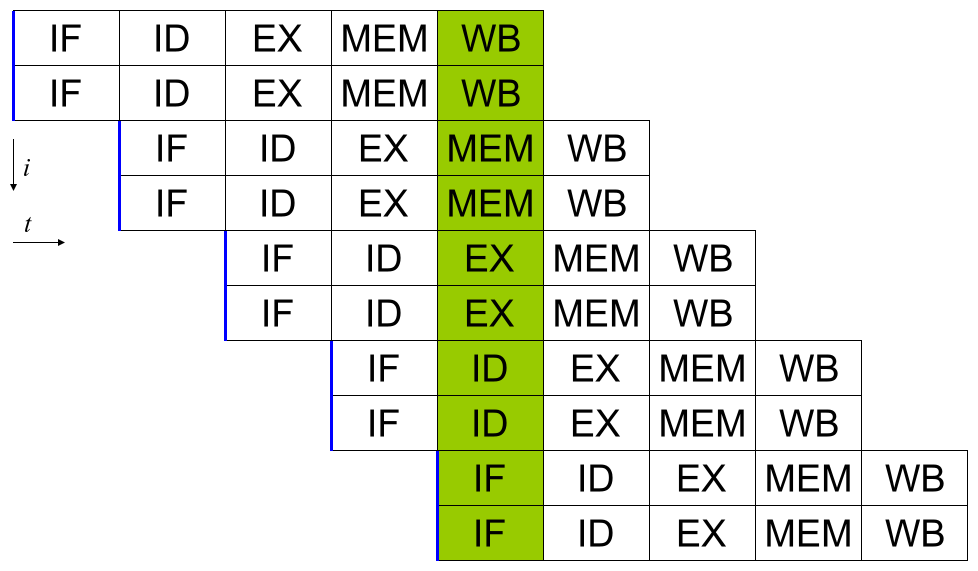
\includegraphics[width=7cm]{images/Chapitre1/superscalar.png}
    \caption{\label{pic_superscalar} Exemple d'un processeur a 2 pipeline (source \url{https://en.wikipedia.org/wiki/Superscalar_processor}) }
\end{figure}

Executer plus d'une instruction par cycle
Cool si on arrive a apport des instructions indépendantes
Exemple du sandy bridge these papier
PAr exemple requete memoire en meme temps que un calcul

Programmer: donner un exemple de si on interlive un code ou non (PAtrick ? ) ou celui page 21














%%%%%%%%%%%%%%%%%%%%%%%%%%%%%%%%%%%%%%%%%%%%%%%%%%%%%%%%%%%%%%%
%%%%%%%%%%%%%%%%%%%%%%%%%%%%%%%%%%%%%%%%%%%%%%%%%%%%%%%%%%%%%%%
\subsection{Processeur vectoriel}
\begin{fancyquotes}
Un processeur vectoriel travaille sur un groupe de données indépendantes Les opérandes sont alors stockées dans des registres vectoriels capable de charger un vecteur pour y appliquer une même opération \cite{hughes2015single}
\end{fancyquotes}

 En effet dans les années 90, les ordinateurs personnels commencés à être utilisé pour lire des vidéos ou de la musique. Dans le but d'augmenter la performance de ces applications multimédia mais aussi d'augmenter les performances des processeurs tout en ne consommant pas plus d'énergie les architectes ont voulu améliorer l'efficacité d'une instruction en implémentant des architectures SIMD (\textit{Single Instruction Multiple Data} de la taxonomie de Flynn \label{sub_taxonomie}).Le principe est d'exécuter une instruction non pas sur une donnée comme le font les processeurs dit scalaires, mais sur un ensemble de données communément appelées vecteur (figure \ref{pic_simd}).
 
 

\begin{figure}
    \center
    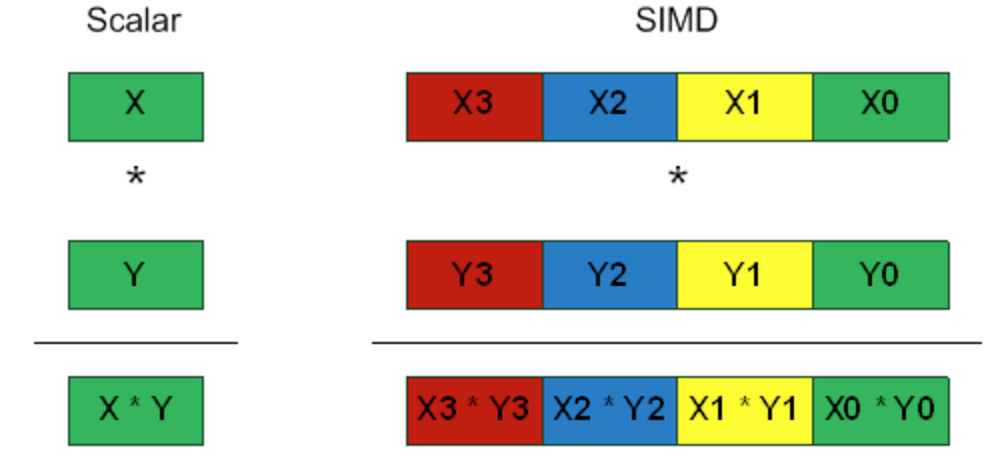
\includegraphics[width=7cm]{images/Chapitre1/simd.png}
    \caption{\label{pic_simd} Schéma de fonctionnement d'une multiplication vectorielle (\url{https://software.intel.com/en-us/articles/ticker-tape-part-2}}
\end{figure}

 
 C'est en 1995 que Sun Microsystem introduit son premier jeu d'instruction vectoriel, le \textit{Visual Instruction Set} auquel Intel répondra en 1997 avec son processeur Pentium MMX et son jeu d'instructions du même nom. Ainsi ces instructions pouvaient réaliser des opérations sur les jeux de données tel que les images ou vidéos de façon très performante. En 1997 AMD viendra améliorer le jeu d'instruction MMX avec l'implémentions des instructions \textit{3DNow!} qui rendait alors possible les opérations vectoriels sur les nombre flottant. La possibilité de faire une opération sur deux nombre flottant par cycle doublait alors la performance des processeurs. Intel répondit alors à cette avancé avec le jeu d'instructions Streaming SIMD Extensions (SSE) en 1999. Il est alors facile d'augmenter la puissance des processeurs: il suffit d'augmenter la taille des vecteurs. Au plus ils pourront appliquer les instructions sur de données, au plus grand sera le nombre de FLOP par cycle réalisés. Les versions suivantes des jeu d'instructions vectorielles ne feront que continuer dans ce sens en utilisant des processeurs avec plus de registres vectoriels mais aussi de taille plus grande (voir \ref{tab_simd}).
 
 
 

\begin{table}[]
\centering
\caption{Évolutions principales des instructions SIMD de $x86$}
\label{tab_simd}
\begin{tabular}{|l|l|l|l|l|l|}
\hline
\multicolumn{1}{|c|}{\textbf{Année}} & \multicolumn{1}{c|}{\textbf{Nom}} & \multicolumn{1}{c|}{\textbf{Nb registres}} & \multicolumn{1}{c|}{\textbf{Taille (bit)}} & \multicolumn{1}{c|}{\textbf{Registres}} & \multicolumn{1}{c|}{\textbf{Commentaires}} \\ \hline
1996                                 & MMX                               & 8                                          & 64                                         & MM0                                     & Nombre entiers
\\ \hline
1999                                 & SSE                               & 8                                          & 128                                        & XMM0                                    & 120 instr., simple precisions              \\ \hline
2006                                 & SSSE3                             & 8                                          & 128                                        & XMM0                                    & 300 instr., double précisions              \\ \hline
2008                                 & AVX                               & 16                                         & 128                                        & XMM0                                    & FMA4, op. a 3 opérandes                    \\ \hline
2011                                 & AVX2                              &  16                                          & 256                                        & YMM0                                    &                                            \\ \hline
2013                                 & AVX512                            & 32                                         & 512                                        & ZMM                                     & FMA3                                       \\ \hline
\end{tabular}
\end{table}

\begin{figure}
    \center
    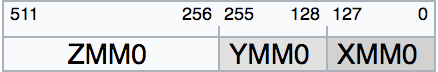
\includegraphics[width=7cm]{images/Chapitre1/simd_registres.png}
    \caption{\label{pic_simd_registres} Découpage d'un registre de 512 bits}
\end{figure}


 Aussi, utiliser des instructions vectorielles permet de s'assurer que la bande passante utilisé l'est pour des données utiles. A la différence d'instruction scalaire ou le processeur doit charger une \textit{cache line} avec des données pas toujours utiles, utiliser des instructions vectorielles force le développeur à repenser ses structures de données.


Cependant, dans la pratique les codes ne sont pas aussi parallèle que nous le souhaiterions et certains aspect du code empêche de tirer la totalité de la performance disponible. En effet, si les données sont indépendantes les unes des autres, il est alors impossible de les calculer simultanément rendant la partie vectorielle inutilisable. Aussi les performances peuvent  être réduites si les données accédées ne sont pas continues en mémoire.  Cela demande donc un travail supplémentaire pour repenser les structures de données et s'assurer que les donnés transférées sur le bus mémoire sont des données \textit{utiles} (voir le concept de ligne de cache TODO ref). Par exemple le calcul vectoriel ne s'appliquera pas sur une structure de données irrégulière comme un tableau de \textit{structures}. Enfin, cette amélioration réduit la pression que subit l'unité responsable du \textit{fetch} et du \textit{decode}. Car avec une seule instruction vectorielle, le processeur réalise le travaille de plusieurs instructions scalaires qui n'auront pas besoin d'être décodées. Il en résulte que doubler largeur des instructions revient à doubler le nombre de FLOP réalisable par le processeur alors que la consommation électrique augmentera d'un facteur inférieur à 2. Beaucoup d'efforts ont donc été réalisé pour être capable d'utiliser cette technologie, par exemple la majorité des compilateurs est capable de détecter les zones de codes parallélisable pouvant bénéficier d'instructions SIMD.





%%%%%%%%%%%%%%%%%%%%%%%%%%%%%%%%%%%%%%%%%%%%%%%%%%%%%%%%%%%%%%%%%%%%
%%%%%%%%%%%%%%%%%%%%%%%%%%%%%%%%%%%%%%%%%%%%%%%%%%%%%%%%%%%%%%%%%%%%
\subsection{Processeur multi-cœur}
2000 Netburst architecture - 2000
The architecture of modern CPUs is largely dictated by the fact that getting data from memory is much
slower than processing it. Hence, a hierarchy of ever faster and smaller tries to keep data as close to the
processing unit as possible, mitigating the long latency and small bandwidth of main memory. The ILP in
the processing unit also helps to hide the latency and more fully utilize the available bandwidth.

%%%%%%%%%%%%%%%%%%%%%%%%%%%%%%%%%%%%%%%%%%%%%%%%%%%%%%%%%%%%%%%%%%%%
%%%%%%%%%%%%%%%%%%%%%%%%%%%%%%%%%%%%%%%%%%%%%%%%%%%%%%%%%%%%%%%%%%%%
\subsubsection{Intel Hyperthreading \copyright}

Hyperthreading, on the other hand, refers to a very specific hardware technology created by Intel, which allows a single processor core to interleave multiple threads of execution more efficiently. In other words, a CPU with hyperthreading is going to provide performance which is somewhat greater than a CPU which is otherwise the same but without hyperthreading, because the hyperthreaded CPU will be able to concurrently balance two (sometimes more, but hyperthreading is usually 2-way) threads of execution on a given core.

Hyper-threading enables a single processor core to be used for two or more concurrent executions with just a little extra hardware.

 

%%%%%%%%%%%%%%%%%%%%%%%%%%%%%%%%%%%%%%%%%%%%%%%%%%%%%%%%%%%%%%%%%%%%
%%%%%%%%%%%%%%%%%%%%%%%%%%%%%%%%%%%%%%%%%%%%%%%%%%%%%%%%%%%%%%%%%%%%
\subsection{Multiprocesseur symétrique (SMP) }
2006 Core architecture
Les system équipé de processeurs identiques.

\subsubsection{Lien QPI}
\subsubsection{NUMA}
2006 Core Architecture



%%%%%%%%%%%%%%%%%%%%%%%%%%%%%%%%%%%%%%%%%%%%%%%%%%%%%%%%%%%%%%%%%%%%
%%%%%%%%%%%%%%%%%%%%%%%%%%%%%%%%%%%%%%%%%%%%%%%%%%%%%%%%%%%%%%%%%%%%
\subsection{Les fréquences}
\subsubsection{Turbo}
2011 Sandy Bridge Architecture
	Turbo Boost

At the same time, the focus on uniprocessor performance was shifting to clock speed. In the mid-to-late 1990s clock frequency increases in general-purpose processors accelerated dra matically. Manufacturers of desktop processors oftencompeted directly on clock frequency rather than actual performance. For programmers, this was fantastic—getting much better performance automatically across generations meant less effort was needed on code optimization. However, this was short-lived. In the early 2000s, this clock frequency war ended rather abruptly as pro cessor designers were reined in by physical constraints—clock frequency increases had drastically increased processor power consumption, and this was stressing cooling technology, not to men tion battery life of the increasingly important laptops.

%%%%%%%%%%%%%%%%%%%%%%%%%%%%%%%%%%%%%%%%%%%%%%%%%%%%%%%%%%%%%%%%%%%%
%%%%%%%%%%%%%%%%%%%%%%%%%%%%%%%%%%%%%%%%%%%%%%%%%%%%%%%%%%%%%%%%%%%%
\subsection{Les accélérateurs}
Creation de processeur spécific a certains besoins

\subsubsection{PCI Express}

\subsubsection{GPU}

\subsubsection{FPGA}


%%%%%%%%%%%%%%%%%%%%%%%%%%%%%%%%%%%%%%%%%%%%%%%%%%%%%%%%%%%%%%%%%%%%
%%%%%%%%%%%%%%%%%%%%%%%%%%%%%%%%%%%%%%%%%%%%%%%%%%%%%%%%%%%%%%%%%%%%
%%%%%%%%%%%%%%%%%%%%%%%%%%%%%%%%%%%%%%%%%%%%%%%%%%%%%%%%%%%%%%%%%%%%
%%%%%%%%%%%%%%%%%%%%%%%%%%%%%%%%%%%%%%%%%%%%%%%%%%%%%%%%%%%%%%%%%%%%
%%%%%%%%%%%%%%%%%%%%%%%%%%%%%%%%%%%%%%%%%%%%%%%%%%%%%%%%%%%%%%%%%%%%
%%%%%%%%%%%%%%%%%%%%%%%%%%%%%%%%%%%%%%%%%%%%%%%%%%%%%%%%%%%%%%%%%%%%
%%%%%%%%%%%%%%%%%%%%%%%%%%%%%%%%%%%%%%%%%%%%%%%%%%%%%%%%%%%%%%%%%%%%
%%%%%%%%%%%%%%%%%%%%%%%%%%%%%%%%%%%%%%%%%%%%%%%%%%%%%%%%%%%%%%%%%%%%
%%%%%%%%%%%%%%%%%%%%%%%%%%%%%%%%%%%%%%%%%%%%%%%%%%%%%%%%%%%%%%%%%%%%
%%%%%%%%%%%%%%%%%%%%%%%%%%%%%%%%%%%%%%%%%%%%%%%%%%%%%%%%%%%%%%%%%%%%
%%%%%%%%%%%%%%%%%%%%%%%%%%%%%%%%%%%%%%%%%%%%%%%%%%%%%%%%%%%%%%%%%%%%
%%%%%%%%%%%%%%%%%%%%%%%%%%%%%%%%%%%%%%%%%%%%%%%%%%%%%%%%%%%%%%%%%%%%
%%%%%%%%%%%%%%%%%%%%%%%%%%%%%%%%%%%%%%%%%%%%%%%%%%%%%%%%%%%%%%%%%%%%
%%%%%%%%%%%%%%%%%%%%%%%%%%%%%%%%%%%%%%%%%%%%%%%%%%%%%%%%%%%%%%%%%%%%
%%%%%%%%%%%%%%%%%%%%%%%%%%%%%%%%%%%%%%%%%%%%%%%%%%%%%%%%%%%%%%%%%%%%
%%%%%%%%%%%%%%%%%%%%%%%%%%%%%%%%%%%%%%%%%%%%%%%%%%%%%%%%%%%%%%%%%%%%
%%%%%%%%%%%%%%%%%%%%%%%%%%%%%%%%%%%%%%%%%%%%%%%%%%%%%%%%%%%%%%%%%%%%
%%%%%%%%%%%%%%%%%%%%%%%%%%%%%%%%%%%%%%%%%%%%%%%%%%%%%%%%%%%%%%%%%%%%


\section{Évolution des mémoires}

\subsection{La mémoire virtuelle}
\label{sub_virtual_mem}

\subsubsection{Historique technologique}
RAM, SRAM, DRAM, NAND/NOR flash

\subsection{La hiérarchie mémoire}
\subsubsection{Principe de localité}

\subsubsection{Caches}
\subsubsection{Politiques}
coherence
remplacement
caching


%%%%%%%%%%%%%%%%%%%%%%%%%%%%%%%%%%%%%%%%%%%%%%%%%%%%%%%%%%%%%%%%%%%%
%%%%%%%%%%%%%%%%%%%%%%%%%%%%%%%%%%%%%%%%%%%%%%%%%%%%%%%%%%%%%%%%%%%%
%%%%%%%%%%%%%%%%%%%%%%%%%%%%%%%%%%%%%%%%%%%%%%%%%%%%%%%%%%%%%%%%%%%%
%%%%%%%%%%%%%%%%%%%%%%%%%%%%%%%%%%%%%%%%%%%%%%%%%%%%%%%%%%%%%%%%%%%%
%%%%%%%%%%%%%%%%%%%%%%%%%%%%%%%%%%%%%%%%%%%%%%%%%%%%%%%%%%%%%%%%%%%%
%%%%%%%%%%%%%%%%%%%%%%%%%%%%%%%%%%%%%%%%%%%%%%%%%%%%%%%%%%%%%%%%%%%%
%%%%%%%%%%%%%%%%%%%%%%%%%%%%%%%%%%%%%%%%%%%%%%%%%%%%%%%%%%%%%%%%%%%%
%%%%%%%%%%%%%%%%%%%%%%%%%%%%%%%%%%%%%%%%%%%%%%%%%%%%%%%%%%%%%%%%%%%%
%%%%%%%%%%%%%%%%%%%%%%%%%%%%%%%%%%%%%%%%%%%%%%%%%%%%%%%%%%%%%%%%%%%%
%%%%%%%%%%%%%%%%%%%%%%%%%%%%%%%%%%%%%%%%%%%%%%%%%%%%%%%%%%%%%%%%%%%%
%%%%%%%%%%%%%%%%%%%%%%%%%%%%%%%%%%%%%%%%%%%%%%%%%%%%%%%%%%%%%%%%%%%%
%%%%%%%%%%%%%%%%%%%%%%%%%%%%%%%%%%%%%%%%%%%%%%%%%%%%%%%%%%%%%%%%%%%%
%%%%%%%%%%%%%%%%%%%%%%%%%%%%%%%%%%%%%%%%%%%%%%%%%%%%%%%%%%%%%%%%%%%%
%%%%%%%%%%%%%%%%%%%%%%%%%%%%%%%%%%%%%%%%%%%%%%%%%%%%%%%%%%%%%%%%%%%%
%%%%%%%%%%%%%%%%%%%%%%%%%%%%%%%%%%%%%%%%%%%%%%%%%%%%%%%%%%%%%%%%%%%%
%%%%%%%%%%%%%%%%%%%%%%%%%%%%%%%%%%%%%%%%%%%%%%%%%%%%%%%%%%%%%%%%%%%%
%%%%%%%%%%%%%%%%%%%%%%%%%%%%%%%%%%%%%%%%%%%%%%%%%%%%%%%%%%%%%%%%%%%%
%%%%%%%%%%%%%%%%%%%%%%%%%%%%%%%%%%%%%%%%%%%%%%%%%%%%%%%%%%%%%%%%%%%%





\section{Le parallélisme}
There is the theoretical question of the absolutely maximum number of actions that can be taken in parallel, but we also need to wonder what kind of actions these are and how hard it is to actually execute them in parallel, as well has how efficient the resulting execution is.




%%%%%%%%%%%%%%%%%%%%%%%%%%%%%%%%%%%%%%%%%%%%%%%%%%%%%%%%%%%%%%%
%%%%%%%%%%%%%%%%%%%%%%%%%%%%%%%%%%%%%%%%%%%%%%%%%%%%%%%%%%%%%%%

\subsection{Le calcul parallèle}
\label{sub_reso_partage} 

Exécuter plusieurs fois le même programme n'est souvent pas très utile car si on ne changeait pas le codes, les données ou les paramètres d'entrées il donnerait le même résultat (aux erreurs d'arrondissement près). Le but principale du calcul parallèle est donc d'exécuter les programme plus rapidement. Pour pouvoir exécuter ce code en parallèle il faut apporter des modifications à un code qui a été pensé pour tourner de manière séquentiel. L'ajout simple de plusieurs processeurs ne suffit pas. Le programmeur peut donc apporter les modifications lui même au code en utilisant un langage prévu pour ou utiliser un compilateur qui va automatiquement généré le code pour les parties qui peuvent en bénéficier. 


 Prenons un exemple d'un problème qui peut être calculé grâce à cette méthode: l'approximation de $\pi$ par le calcul de l'intégral \ref{eq_pi}.
\begin{equation}
\label{eq_pi}
\int_{0}^{1} \frac{4.0}{1 + x^{2}}
\end{equation}
Calculer une intégrale revient à calculer l'air formé par cette courbe et l'axe des abscisse dans le domaine étudié, ici $[0,1]$. Comme la courbe dessinée par cette formule est sinusoïdale, le calcul de sa surface est impossible. On peut essayer de calculer cette surface par une méthode très connue sous le nom d'approximation par la méthode des rectangle (ou trapèze).
Cela reviens à dessiner des rectangles sous la courbes et de calculer la surface correspondante. La surface d'un rectangle étant calculable, on pourra donc trouver une approximation de la surface recherchée. En effet, sur la figure \ref{pic_pi_1}, on voit qu'en calculant et en sommant la surface de tous les rectangles bleus on trouvera un résultat proche de celui de la surface dessiné par la courbe rouge. 

\begin{figure}[t!]
    \centering
    \begin{subfigure}[t]{0.5\textwidth}
        \label{pic_pi_1}
        \centering
        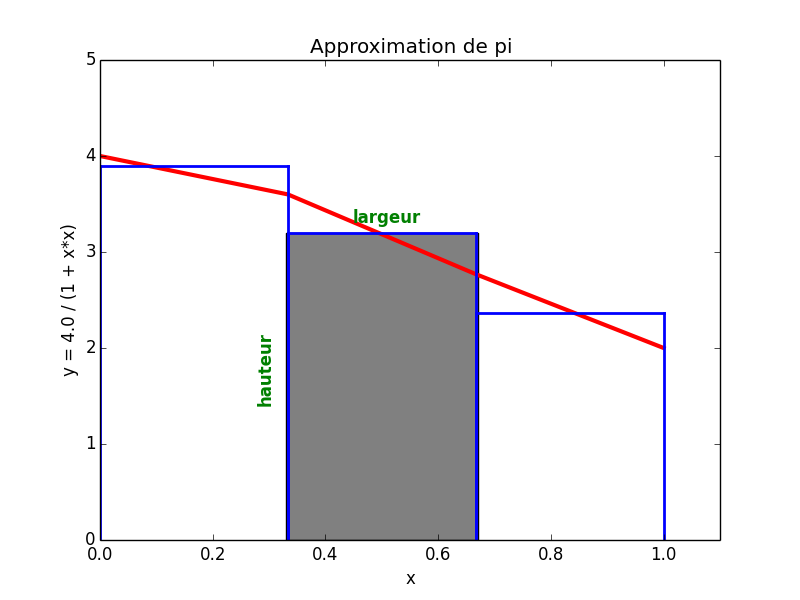
\includegraphics[height=1.8in]{images/Chapitre1/pic_pi_rect_1.png}
        \caption{Approximation avec 4 rectangles}
    \end{subfigure}%
\begin{subfigure}[t]{0.5\textwidth}
        \label{pic_pi_2}
        \centering
        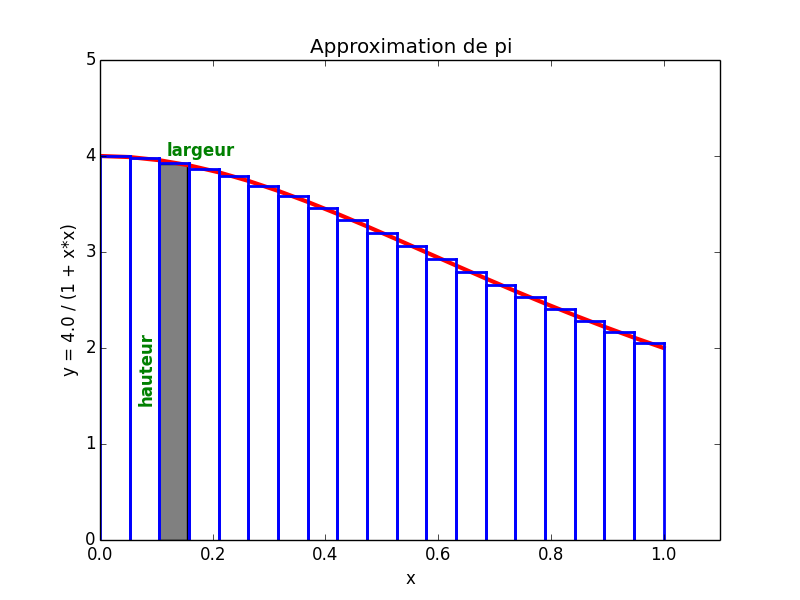
\includegraphics[height=1.8in]{images/Chapitre1/pic_pi_rect_2.png}
        \caption{Approximation avec 14 rectangles}
    \end{subfigure}
    \caption{Méthode des rectangles: exemple de deux exécutions de l'algorithmes un nombre de rectangles différents. Si peu de rectangle sont utilisés cela crée des erreurs. Si on choisit plus de rectangles, on est plus précis, mais plus de ressources sont nécessaires pour le calculer }
    \label{pic_pi_rect}
\end{figure}

\begin{lstlisting}[language=C, caption=Implémentions de l'algorithme de calcul d'intégrale par la méthode des rectangles, float,floatplacement=H]

static long num steps = 100000; 
double step;
void main ()
{
    double largeur, hauteur, pi = 0.0;

    int num_steps = 4;
    //  num_steps = 14;

    largeur = 1.0 / num_steps;

    for (i = 0; i < num_steps; ++i) {
        x =  (i) * step;
        hauteur = ( 4.0/(1.0+x*x));
        pi += largeur * hauteur;
    }
    
    cout << "Valeur de pi: " << pi << endl;

}
\end{lstlisting}



La précision du calcul dépendra du nombre de rectangle choisi, mais approximer l'intégrale avec plus de rectangle demandera plus de ressources informatiques. Si on veut que tous les rectangles soient calculés en même temps il faudra avoir autant de processeurs que de rectangles. C'est un exemple, bien que simpliste, qui montre que la précision des calculs est directement dépendantes du nombre de ressources calculatoire si on veut que le calcul soit résolu dans le même temps. Cet exemple à pour but de montrer que la demande de ressources de calculs est infinis. Dès lors que l'on voudra avoir des résultats plus rapidement, on aura alors besoin d'ordinateurs plus puissants. Et aujourd'hui ces demandes sont réelles, on pourrait évoquer les voitures autonomes qui vont avoir besoin de prendre des décisions en quelques millisecondes. Mais cette logique n'est pas vrai pour un nombre de processeurs infinis et c'est aussi une des motivations de cette thèse. En effet, la loi d'Amdlahl exprime comment la performance est impacté par le nombre de processeurs utilisés.
 



\subsubsection{La loi d'Amdahl} 

\paragraph{La scalabilité TODO}
To get good speedup on a multiprocessor while keeping the problem size fixed is harder than getting good speedup by increasing the size of the problem
Strong scaling:  When speedup is achieved on a parallel processor without increasing the size of the problem
Weak scaling:  When speedup is achieved on a parallel processor by increasing the size of the problem proportionally to the increase in the number of processors

strong
weak

 Il est  souvent impossible de réduire le temps d'exécution du même facteur que le nombre de machines dont on dispose. En effet, les codes comporteront toujours des parties dites séquentiels qui ne peuvent pas être exécutées en parallèle. L'accélération de l'exécution en fonction de la taille de ces parties séquentiels peut être exprimé avec la loi d'Amdahl.

Elle exprime l'accélération du temps d'exécution que l'on peut espérer en fonction des portions de codes qui peuvent être exécuté en parallèle (\autoref{eq_amdahl}). En 1960, Gene Amdahl explique que même si 99\% du code était exécutable en parallèle l'accélération de ce code serait limitée et cela sans regard du nombre de processeurs disponibles. Dans cette équation $P$ représente la portion de code qui peut être exécutée en parallèle et $N$ le nombre de processeurs disponibles.

\begin{equation}
\label{eq_amdahl}
    Speedup (N) = \frac{1}{(1-P) + \frac{P}{N}}
\end{equation}

\begin{figure}
    \center
    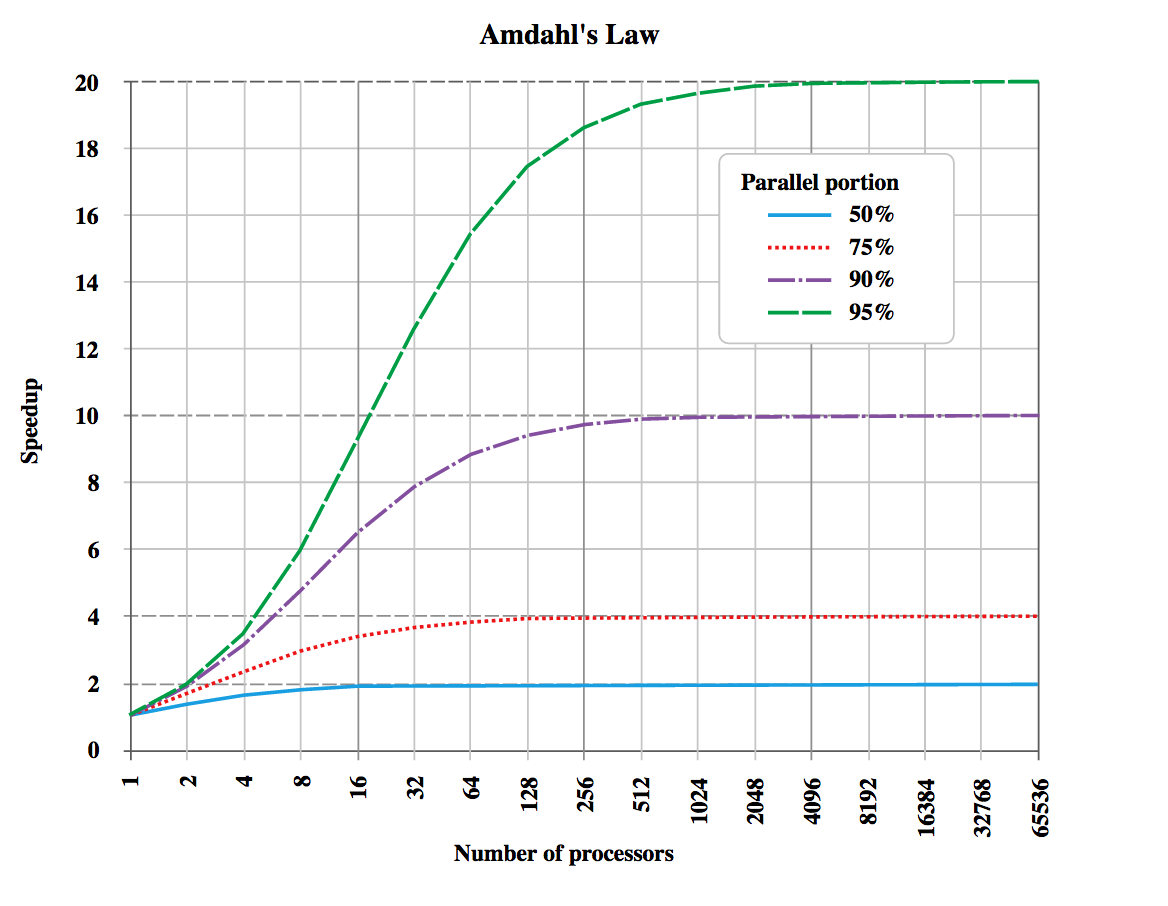
\includegraphics[width=10cm]{images/Chapitre1/AmdahlsLaw.png}
    \caption{\label{pic_amdahl} La loi d'Amdahl décrit l'accélération théorique en fonction du nombre de processeurs pour des codes avec des zones parallèles de différentes taille (source \url{https://fr.wikipedia.org/wiki/Loi\_d\%27Amdahl}).}
\end{figure}

\paragraph{Loi de Gustafson TODO}

TODO faire référence aux different niveaux de parallelisme Taxonomie etc...










%%%%%%%%%%%%%%%%%%%%%%%%%%%%%%%%%%%%%%%%%%%%%%%%%%%%%%%%%%%%%%%
%%%%%%%%%%%%%%%%%%%%%%%%%%%%%%%%%%%%%%%%%%%%%%%%%%%%%%%%%%%%%%%
\subsection{Granularité de parallélisme}

\subsubsection{Parallélisme des instructions (ILP)}
Exemple de deux instructions qui peuvent etre executée séparément
ILP - Instruction
	Superscalar
	Aide: unrolling
	
\subsubsection{Parallélisme des données (DLP)}
- Partition the data used in solving the problem among the cores.
–  Each core carries out similar operations on it s part of the data.

DLP - Data
	SIMD vector
	Aide: blocking, squewing
	Parallel data structures
	
MMX SSE...
One of the issues in parallel program design is the use of Array-Of-Structures (AOS) vs Structure-OfArrays
(SOA). In normal program design you often define a structure
	
Data center
MPI
$https://www.polyhedron.com/web_images/intel/productbriefs/3a_SIMD.pdf$

Exemple d'une multiplication de A * B


\subsubsection{Parallélisme de taches (TLP)}
task parallelism is about identifying whole
subprograms that can be executed in parallel. As an example, searching in a tree data structure
Partition various tasks carried out solving the problem among the
cores.


%%%%%%%%%%%%%%%%%%%%%%%%%%%%%%%%%%%%%%%%%%%%%%%%%%%%%%%%%%%%%%%
%%%%%%%%%%%%%%%%%%%%%%%%%%%%%%%%%%%%%%%%%%%%%%%%%%%%%%%%%%%%%%%
\subsection{La programmation parallèle}
La mémoire est plus grande que le nombre de coeurs. On peut pas avoir un process par data. Il faut donc regrouper, faire des sous tableaux. TODO: exemple de repartition BCN tab [i*myrank].

 


\subsubsection{Parallesisme des threads}

\paragraph{}{Les threads}
Definition des thread: thead vs program.Processes can belong to different users, or be different programs that a single user is running concurrently,
so they have their own data space. On the other hand, threads are part of one process and therefore share
the process heap. Threads can have some private data, for instance

The thread mechanism has long existed, even on a single processor. By having more than one thread on
a single processor, a higher processor utilization can result, since the instructions of one thread can be
processed while another thread is waiting for data

Since threads share data, they are one possible mechanism for parallel programming. Of course, for this to be faster than sequential single-threaded execution, this assumes that the hardware can work on more than one thread at the same time. This can happen in two main circumstances: a multicore processor can accomodate one thread per core, and secondly, some cores have hardware support for executing more than one thread.  processor cores can be an easy way to parallelize a
computation. The shared memory allows the threads to all see the same data.

\paragraph{Exemple OpenMP}
$https://hal.archives-ouvertes.fr/hal-01257189/document p97$



\subsubsection{Data races, thread safety, sequential consistency, and atomic operations }






%%%%%%%%%%%%%%%%%%%%%%%%%%%%%%%%%%%%%%%%%%%%%%%%%%%%%%%%%%%%%%%%%%%%
%%%%%%%%%%%%%%%%%%%%%%%%%%%%%%%%%%%%%%%%%%%%%%%%%%%%%%%%%%%%%%%%%%%%
%%%%%%%%%%%%%%%%%%%%%%%%%%%%%%%%%%%%%%%%%%%%%%%%%%%%%%%%%%%%%%%%%%%%
%%%%%%%%%%%%%%%%%%%%%%%%%%%%%%%%%%%%%%%%%%%%%%%%%%%%%%%%%%%%%%%%%%%%
%%%%%%%%%%%%%%%%%%%%%%%%%%%%%%%%%%%%%%%%%%%%%%%%%%%%%%%%%%%%%%%%%%%%
%%%%%%%%%%%%%%%%%%%%%%%%%%%%%%%%%%%%%%%%%%%%%%%%%%%%%%%%%%%%%%%%%%%%
%%%%%%%%%%%%%%%%%%%%%%%%%%%%%%%%%%%%%%%%%%%%%%%%%%%%%%%%%%%%%%%%%%%%
%%%%%%%%%%%%%%%%%%%%%%%%%%%%%%%%%%%%%%%%%%%%%%%%%%%%%%%%%%%%%%%%%%%%
%%%%%%%%%%%%%%%%%%%%%%%%%%%%%%%%%%%%%%%%%%%%%%%%%%%%%%%%%%%%%%%%%%%%
%%%%%%%%%%%%%%%%%%%%%%%%%%%%%%%%%%%%%%%%%%%%%%%%%%%%%%%%%%%%%%%%%%%%
%%%%%%%%%%%%%%%%%%%%%%%%%%%%%%%%%%%%%%%%%%%%%%%%%%%%%%%%%%%%%%%%%%%%
%%%%%%%%%%%%%%%%%%%%%%%%%%%%%%%%%%%%%%%%%%%%%%%%%%%%%%%%%%%%%%%%%%%%
%%%%%%%%%%%%%%%%%%%%%%%%%%%%%%%%%%%%%%%%%%%%%%%%%%%%%%%%%%%%%%%%%%%%
%%%%%%%%%%%%%%%%%%%%%%%%%%%%%%%%%%%%%%%%%%%%%%%%%%%%%%%%%%%%%%%%%%%%
%%%%%%%%%%%%%%%%%%%%%%%%%%%%%%%%%%%%%%%%%%%%%%%%%%%%%%%%%%%%%%%%%%%%
%%%%%%%%%%%%%%%%%%%%%%%%%%%%%%%%%%%%%%%%%%%%%%%%%%%%%%%%%%%%%%%%%%%%
%%%%%%%%%%%%%%%%%%%%%%%%%%%%%%%%%%%%%%%%%%%%%%%%%%%%%%%%%%%%%%%%%%%%
%%%%%%%%%%%%%%%%%%%%%%%%%%%%%%%%%%%%%%%%%%%%%%%%%%%%%%%%%%%%%%%%%%%%



\section{Sommaire}

Alors que nous n'avons jamais eu besoin d'aussi grandes puissances de calcul, le graphique montre bien qu'il y a eu une inflexion en 2012. Le challenge principal inhérent au HPC est celui du cout des machines et donc celui du ratio $\frac{Prix}{FLOPS}$. Un autre challenge qui est apparu est celui de la puissance électrique nécessaire pour aliment les supercalculateurs. Les lignes électrique arrivant sur les sites, ne sont plus assez puissante pour que l'on puisse suivre la stratégie employée jusqu'à aujourd'hui qui était d'augmenter le nombre de machines pour augmenter la puissance de calcul. Aujourd'hui nous cherchons donc aussi à augmenter le ratio $\frac{Watt}{FLOPS}$ même si cette solution ne sera pas éternellement viable comme l'a prédit \cite{5392446}.
Enfin, les clients du HPC acquièrent plus de données que jamais et les clusters doivent pouvoir les contenir et les traiter dans des délais raisonnable. En effet les objets connectés qui génèrent de gigantesques quantité de données doivent être capables d'en traiter une partie sur place avec des moyens souvent limité (énergie, puissance de calculs). Ces challenges sont donc applicables au data center mais aussi à l'extérieur si nous voulons être capable de prendre des décisions en temps réel, comme pour les voitures autonomes qui n'auront que quelques micro secondes pour réagir en cas d'accident. Le travail présenté dans cette thèse est donc nécessaire pour pouvoir accéder à toutes ces promesses que nous réserve l'avenir.


\subsubsection{Systèmes non-équilibrés}

La précision des simulations, les approches multi-physique ainsi que les objets connectés produisent des volumes de données à gérer et à analyser tels qu’ils ont été caractérisé par la communauté de déluge %\cite{bodin:hal-01174302}.
En conséquence, l’exploitation et la gestion des données sont l’autre pan de l’évolution des logicielles qui va bouleverser les pratiques. Une majorité des applications HPC autrefois centrée sur une problématique de puissance de calcul sont maintenant fortement limitées par le traitement des données pour deux raisons: une augmentation très forte de la puissance des processeurs contre une faible augmentation de la quantité de données que les mémoires peuvent leur délivrer. Si on regarde l'évolution des performances des différentes parties du système on peut constater de réelles différences:
\begin{itemize}
    \item Les performances calculatoirs des processeurs (le nombre d'opération flotantes réalisables par cycle) à \textbf{augmenté de 50\%} en moyenne par an.
    \item La bande passante entre le processeur et la mémoire à augmenté de 23\% par an
    \item La lantence des requêtes mémoire a \textbf{augmenté de 4\% }par an
    \item La bande passante sur le réseau à \textbf{augmenté de 20\%} par an
\end{itemize}

\begin{figure}
    \center
    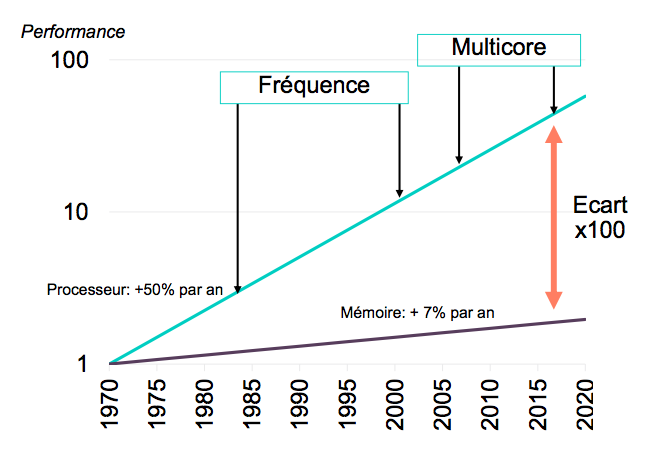
\includegraphics[width=10cm]{images/Chapitre1/memory_gap.png}
    \caption{\label{pic_memory_gap} Différence de l'évolution des performances des processeurs et des mémoires }
\end{figure}

On voit donc que la puissance des processeurs à augmenté bien plus rapidement que celle des mémoires. Les processeurs ont béféniciés de nombreuse amélioration. L'augmentation de la fréquences par exemple, ou le nombre de coeurs par processeur. Ainsi les performances des systèmes ne sont plus équilibrées et les architectures ont du s'adapter notamment avec l'apparition d'une hierarchie mémoire, plus au moins rapide et plus ou moins grande. L'apparition des caches à permis d'augmenter la performance relative des applications en camouflant l'augmentation faible de la bande passante. Cela à contribué à l'augmentation de la complexité des architectures et il faut désormais au programmeur des connaissances solides pour aller tirer le maximum de performances de ces processeurs

\textbf{TODO: annoncer le plan de these}



%%%%%%%%%%%%%%%%%%%%%%%%%%%%%%%%%%%%%%%%%%%%%%%%%%%%%%%%%%%%%%%%%%%%
%%%%%%%%%%%%%%%%%%%%%%%%%%%%%%%%%%%%%%%%%%%%%%%%%%%%%%%%%%%%%%%%%%%%
%%%%%%%%%%%%%%%%%%%%%%%%%%%%%%%%%%%%%%%%%%%%%%%%%%%%%%%%%%%%%%%%%%%%
%%%%%%%%%%%%%%%%%%%%%%%%%%%%%%%%%%%%%%%%%%%%%%%%%%%%%%%%%%%%%%%%%%%%
%%%%%%%%%%%%%%%%%%%%%%%%%%%%%%%%%%%%%%%%%%%%%%%%%%%%%%%%%%%%%%%%%%%%
%%%%%%%%%%%%%%%%%%%%%%%%%%%%%%%%%%%%%%%%%%%%%%%%%%%%%%%%%%%%%%%%%%%%
%%%%%%%%%%%%%%%%%%%%%%%%%%%%%%%%%%%%%%%%%%%%%%%%%%%%%%%%%%%%%%%%%%%%
%%%%%%%%%%%%%%%%%%%%%%%%%%%%%%%%%%%%%%%%%%%%%%%%%%%%%%%%%%%%%%%%%%%%
%%%%%%%%%%%%%%%%%%%%%%%%%%%%%%%%%%%%%%%%%%%%%%%%%%%%%%%%%%%%%%%%%%%%
%%%%%%%%%%%%%%%%%%%%%%%%%%%%%%%%%%%%%%%%%%%%%%%%%%%%%%%%%%%%%%%%%%%%
%%%%%%%%%%%%%%%%%%%%%%%%%%%%%%%%%%%%%%%%%%%%%%%%%%%%%%%%%%%%%%%%%%%%
%%%%%%%%%%%%%%%%%%%%%%%%%%%%%%%%%%%%%%%%%%%%%%%%%%%%%%%%%%%%%%%%%%%%
%%%%%%%%%%%%%%%%%%%%%%%%%%%%%%%%%%%%%%%%%%%%%%%%%%%%%%%%%%%%%%%%%%%%
%%%%%%%%%%%%%%%%%%%%%%%%%%%%%%%%%%%%%%%%%%%%%%%%%%%%%%%%%%%%%%%%%%%%
%%%%%%%%%%%%%%%%%%%%%%%%%%%%%%%%%%%%%%%%%%%%%%%%%%%%%%%%%%%%%%%%%%%%
%%%%%%%%%%%%%%%%%%%%%%%%%%%%%%%%%%%%%%%%%%%%%%%%%%%%%%%%%%%%%%%%%%%%
%%%%%%%%%%%%%%%%%%%%%%%%%%%%%%%%%%%%%%%%%%%%%%%%%%%%%%%%%%%%%%%%%%%%
%%%%%%%%%%%%%%%%%%%%%%%%%%%%%%%%%%%%%%%%%%%%%%%%%%%%%%%%%%%%%%%%%%%%




TODO 
\label{sub_taxonomie}
%\cite{Flynn:1972:COE:1952456.1952459}
$https://www.polyhedron.com/web_images/intel/productbriefs/3a_SIMD.pdf$
schéma nombre d'opération par cycle et aussi que 4xfloat = 2 double = 16xbytes ...

\printbibliography[heading=references,segment=\therefsegment]


%% PART 2 %%
\part{État de l'art}

Partie état de l'art qui rappelle les fondamentaux des processeurs et des logiciels.

\chapter{Architecture des processeurs}
\label{chap:sota:materiel}
\minitoc

\textit{À l'attention du relecteur: ce chapitre fait partie de l'état de l'art de la thèse. Il fait suite à l'introduction qui présente la thèse, ses contributions et ses principaux résultats. La partie état de l'art possède deux chapitres. Celui-ci, et un chapitre concernant le HPC et l'analyse de performance.}\\


L'objectif de ce chapitre est de présenter l'évolution de l'architecture des processeurs et leurs principales évolutions qui sont nécessaires pour réaliser le travail d'analyse de performance étudié dans cette thèse. 
Pour ce faire, le chapitre commence par faire l'historique des processeurs (\autoref{sec:von}) en présentant les premiers calculateurs automatisés ainsi que les débuts de l'architecture Von Neumann à la base de la majorité des processeurs actuels. 
La suite du chapitre est consacrée à l'étude de cette architecture et des principales améliorations qu'elle a reçues ces cinquante dernières années. Pour les présenter, le chapitre regroupe les concepts pour les empiler progressivement à la manière du modèle OSI   \cite{day1983osi}. Pour les besoins de la thèse, les deux premiers niveaux sont présentés dans ce chapitre:
\begin{itemize}
    \item Niveau 1 - Le circuit logique 
        \begin{itemize}
        \item Les transistors et les portes logiques (\autoref{sec:logique})
        \end{itemize}
    \item Niveau 2 - L'architecture 
    \begin{itemize}
        \item La micro-architecture (\autoref{sec:micro})
        \item La hiérarchie mémoire (\autoref{sec:hierarchie})
    \end{itemize}
    \item Niveau 3 - Le système d'exploitation
        \begin{itemize}
            \item La mémoire virtuelle  (\autoref{sec:memoire_virtuelle})
        \end{itemize}
    \item Niveau 4 - Les langages et compilateurs
\end{itemize}

Le lecteur familier au domaine retrouvera beaucoup de concepts connus et peut considérer de passer au chapitre suivant qui s'intéresse au domaine du calcul haute performance et de l'analyse de performance. Lorsque des concepts seront nécessaires dans la partie contribution, un lien sera toujours fait vers la partie correspondante de ce chapitre.



\section{Architecture Von Neumann}

\section{Le circuit logique} \label{sec:logique}
%%%%%%%%%%%%%%%%%%%%%%%%%%%%%%%%%%%%%%%%%%%%%%%%%%%%%%%%%%%%%%%%%%%
%%%%%%%%%%%%%%%%%%%%%%%%%%%%%%%%%%%%%%%%%%%%%%%%%%%%%%%%%%%%%%%%%%%
Le niveau plus bas abordé dans cette thèse est celui des transistors qui sont les composants de bases de tout système électronique. 

\subsection{Les Transistors}
%%%%%%%%%%%%%%%%%%%%%%%%%%%%%%%%%%%%%%%%%%%%%%%%%%%%%%%%%%%%%%%%%%%
Le premier transistor a été mis au point par des chercheurs des Laboratoires Bell en 1947 \cite{bardeen1948transistor} dont la découverte avait été réalisée quelque années avant \cite{edgar1930method}. Ils apparaissent comme une révolution face aux tubes électroniques utilisés jusque là (plus rapide, léger et robuste). Un transistor est un composant électronique qui utilise trois bornes: la base, l’émetteur et le collecteur (voir \autoref{pic:transistor}). Le collecteur est relié au fil d’où vient la tension et correspond à la sortie du transistor. L’émetteur est lui relié à la masse (tension 0 volt). La base constitue la connexion en connecteur et émetteur en fonction de la tension qui lui est appliquée. En appliquant une tension faible à la base, le courant entre le collecteur et l’émetteur est possible. Sans aucune tension appliquée à la base, le passage du courant n’est pas possible. Pour les personnes non familières avec ces concepts électriques, une approche vulgarisée peut être utilisée \cite{JohnLeDuc2017}. Ainsi, le transistor se comporte comme un interrupteur binaire très rapide (basculement en quelques nanosecondes $10^{-9}$ seconde).



\begin{figure}[htbp]
    \centering
    \begin{subfigure}[b]{0.45\linewidth}\centering
        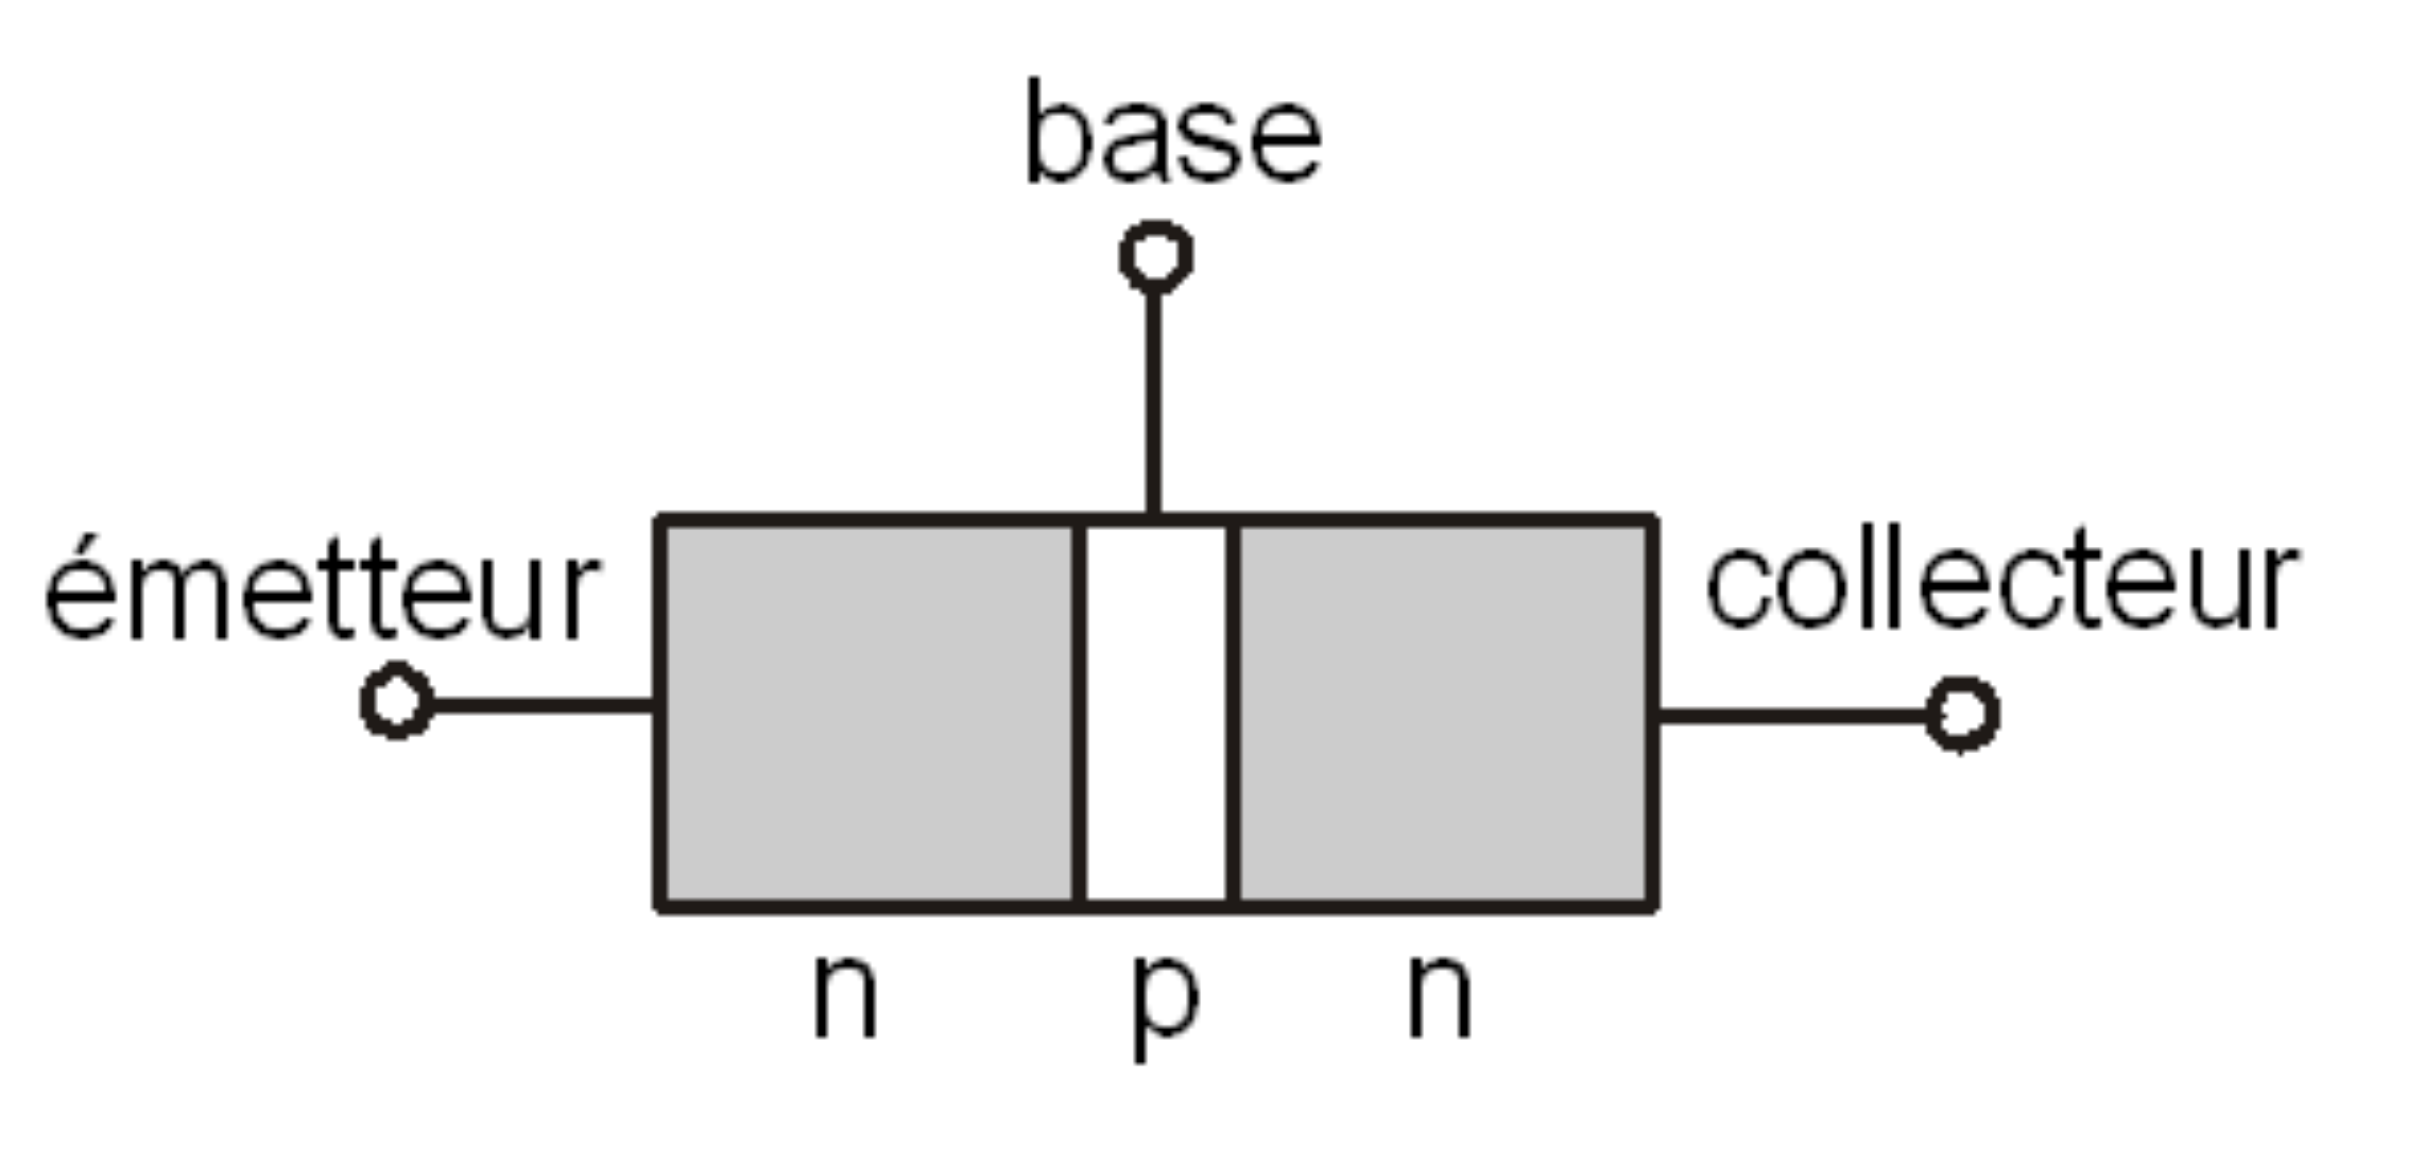
\includegraphics[width=\linewidth]{images/transistor.png}
        \caption{\label{pic:transistor} Schéma d'un transistor NPN \cite{GeraldHuguenin2018}}.
    \end{subfigure}
    ~ %add desired spacing between images, e. g. ~, \quad, \qquad, \hfill etc.
      %(or a blank line to force the subfigure onto a new line)
    \begin{subfigure}[b]{0.45\linewidth}\centering
        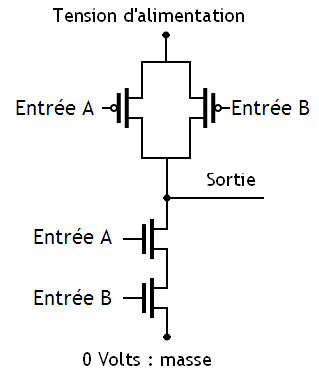
\includegraphics[width=0.5\linewidth]{images/processeur_porte_nand.png}
        \caption{\label{pic:processeur_porte_nand} Schéma électrique d'une porte \textit{NON-ET} réalisée à partir de 4 transistors \cite{Wikibooks2019PorteNand}}
    \end{subfigure}
    \caption{Un transistor est utilisé pour réaliser des portes complexes  }\label{pic:transistor_usage}
\end{figure}




\subsection{Les portes logiques}
%%%%%%%%%%%%%%%%%%%%%%%%%%%%%%%%%%%%%%%%%%%%%%%%%%%%%%%%%%%%%%%%%%%
Les portes logiques sont construites à partir de transistors et permettent l'exécution de différentes instructions ou la capacité de stocker une information (registres). Par exemple, en associant deux transistors inverseur en série on construit une porte NON-ET qui ne laisse passer le courant seulement lorsqu'aucune ou une des deux entrées a une tension (voir \autoref{pic:processeur_porte_nand})



Une porte logique possède plusieurs entrées numériques qui peuvent être le résultat d'autres portes logiques (voir \autoref{pic:processeur_portes}). Les circuits les plus complexes sont en fait une cascade de milliers de portes logiques comme celles-ci. Il est aussi nécessaire de choisir la signification du passage ou non du courant et construire des portes ayant un « sens ». Il est courant d’utiliser les termes VRAI ou \textit{1 logique} lorsque le courant circule et FAUX ou \textit{0 logique} pour l’absence de tension.


\begin{figure}
\begin{subfigure}{.3\textwidth}
\centering

\includegraphics[width=3cm]{images/processeur_porte_et.png}
\caption{La porte \textit{ET} ne laisse passer le courant seulement si les deux entrées sont vraies}
\end{subfigure}\hfill
\begin{subfigure}{.3\textwidth}
\centering

\includegraphics[width=3cm]{images/processeur_porte_ou.png}
\caption{La porte \textit{ET} laisse passer le courant si au moins une des deux entrées est vraies}
\end{subfigure}\hfill
\begin{subfigure}{.3\textwidth}
\centering

\includegraphics[width=3cm]{images/processeur_porte_oux.png}
\caption{La porte \textit{OU EXCLUSIF} est vrai seulement si les deux entrées ont des valeurs distinctes}
\end{subfigure}
\caption{Représentation graphique de trois portes logiques \cite{Wikipedia2019Porte}}
\label{pic:processeur_portes}
\end{figure}




\subsection{Algèbre de Boole}
%%%%%%%%%%%%%%%%%%%%%%%%%%%%%%%%%%%%%%%%%%%%%%%%%%%%%%%%%%%%%%%%%%%
Analyser le fonctionnement de plusieurs portes peut rapidement se complexifier et le recours à des méthodes algébriques est nécessaire. Les portes pouvant avoir des valeurs de 0 ou 1, un nouveau type d'algèbre a été créée: l'algèbre de Boole. Comme pour l'algèbre en base décimale, l'algèbre booléenne utilise des fonctions et des variables pour décrire le comportement d'un système. Les variables utilisées ne peuvent prendre que deux valeurs. Une table de vérité de fonctions générales peut alors être écrite. On peut écrire une table de vérité d'un programme souhaité, qui utilise trois entrées, et déterminer les sorties ($M$) souhaitées (voir \autoref{pic:processeur_porte_table}). Grâce à l'algèbre de Boole, on peut convertir cette table en circuit implémentant ce fonctionnement (\autoref{pic:processeur_porte_schema}).
L'algèbre de Boole est aussi utilisée pour réduire la complexité d'un circuit sans en changer le comportement, notamment grâce à la fameuse loi de DeMorgan \cite{hurley2014concise} permettant le changement de portes \textit{ET} en portes \textit{OU}. En réduisant la complexité et le nombre de portes, il est possible de réaliser des circuits plus économiques et plus rapides.


\begin{figure}[htbp]
    \centering
    \begin{subfigure}[b]{0.40\linewidth}\centering
        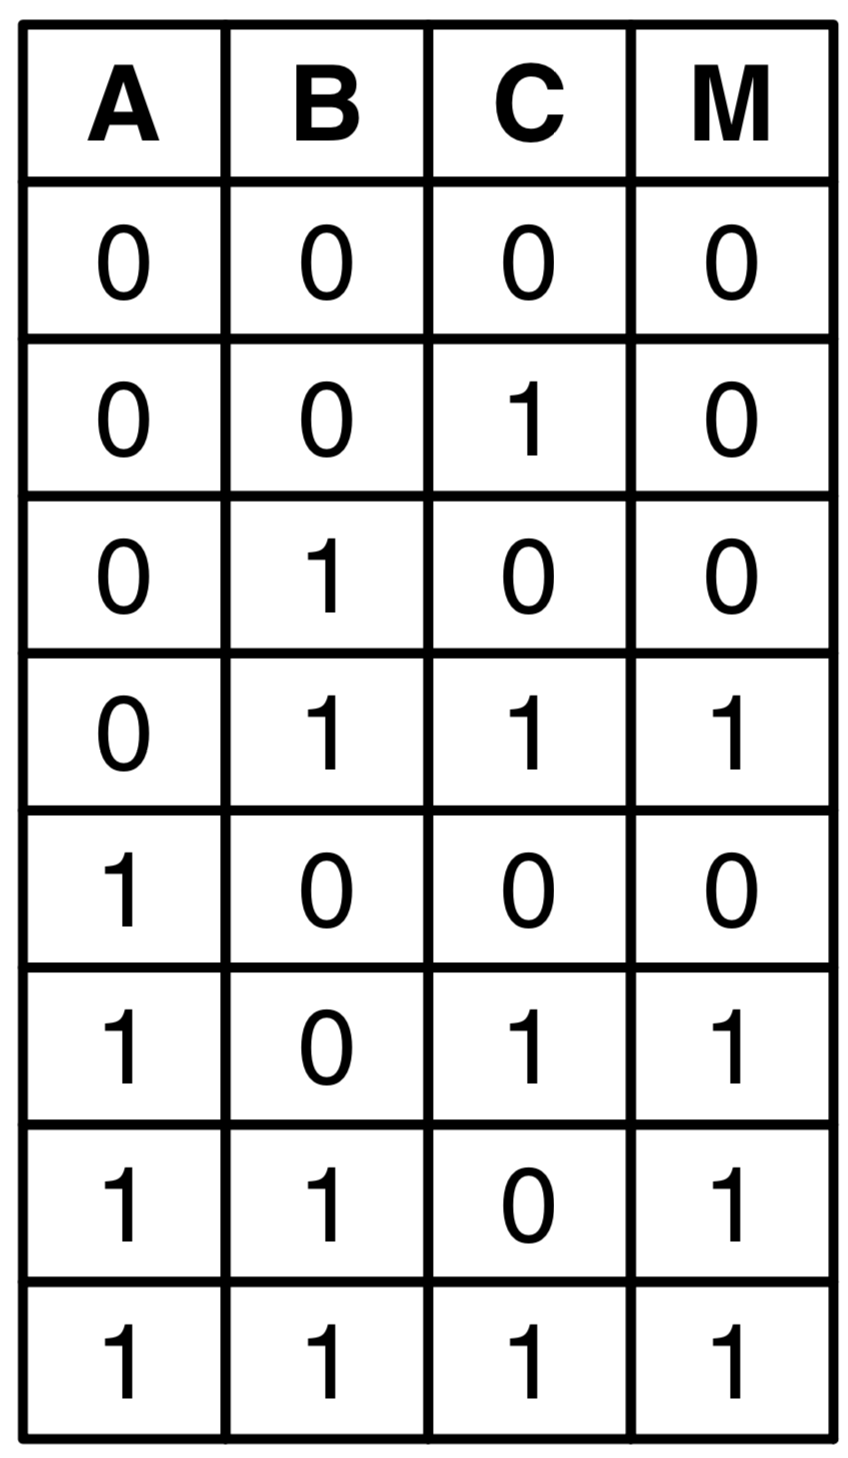
\includegraphics[width=0.4\linewidth]{images/processeur_porte_table.png}
        \caption{Table de vérité d'un circuit souhaité
        \label{pic:processeur_porte_table}}
    \end{subfigure}
    ~ %add desired spacing between images, e. g. ~, \quad, \qquad, \hfill etc.
      %(or a blank line to force the subfigure onto a new line)
    \begin{subfigure}[b]{0.40\linewidth}\centering
        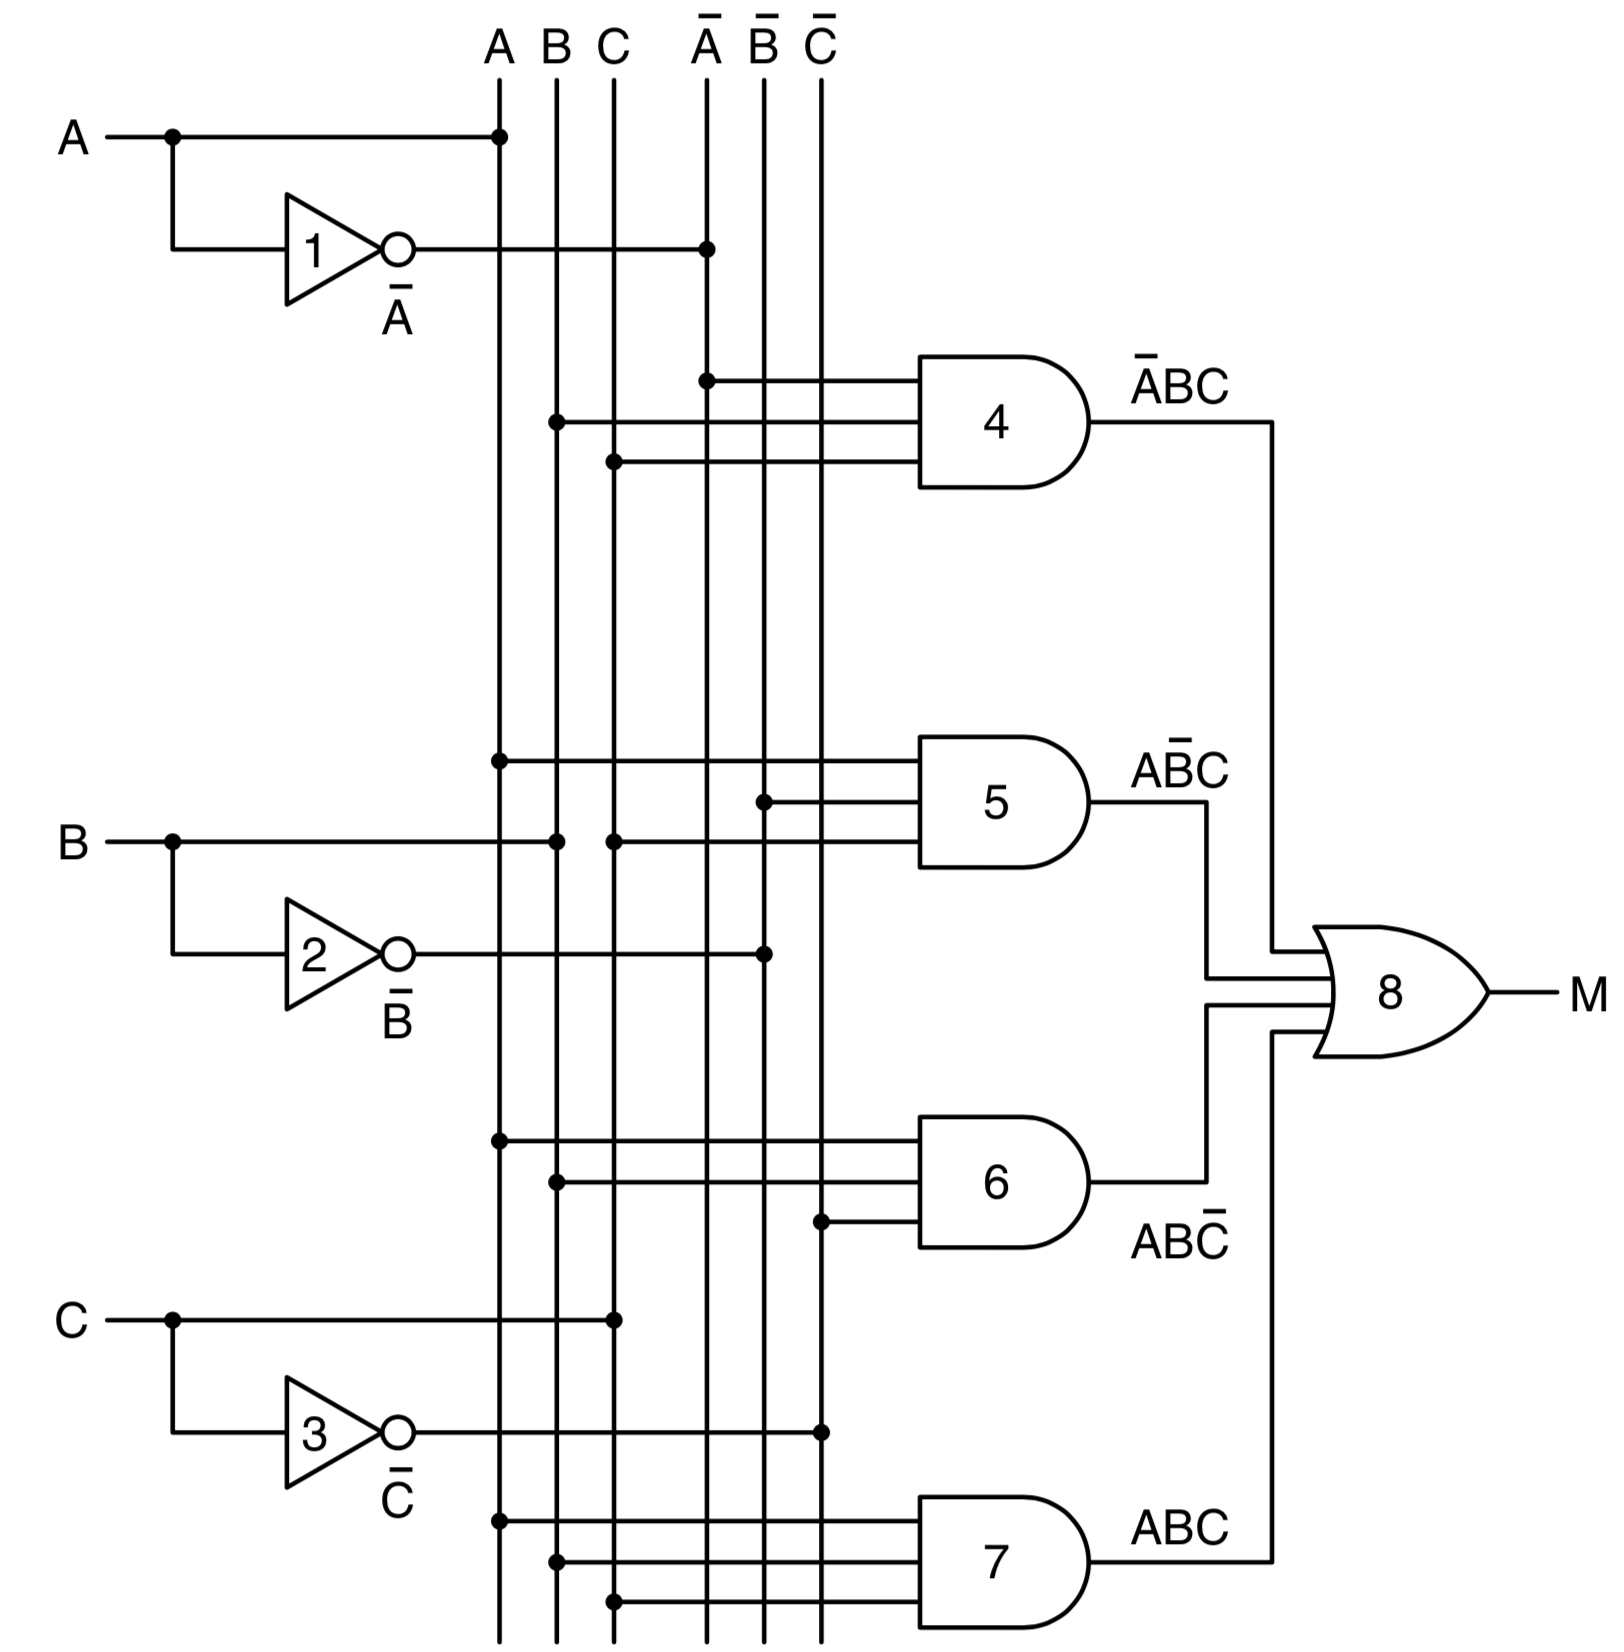
\includegraphics[width=\linewidth]{images/processeur_porte_schema.png}
        \caption{Circuit logiques  utilisant 8 portes
        \label{pic:processeur_porte_schema}}
    \end{subfigure}
    \caption{A partir d'une table de vérité, on peut générer le circuit logique correspondant \cite{tanenbaum2016structured}  \label{pic:processeur_porte_schema}}
\end{figure}




\subsection{Circuits logiques}
%%%%%%%%%%%%%%%%%%%%%%%%%%%%%%%%%%%%%%%%%%%%%%%%%%%%%%%%%%%%%%%%%%%
À partir des portes logiques et de leur analyse avec l'algèbre de Boole des circuits plus complexes peuvent être élaborés qui peuvent être regroupés en deux grandes familles: les circuits logiques de base  et les circuits logiques à mémoire. La principale différence entre les deux vient de leur capacité à retenir une information. 

\subsubsection{Les circuits logiques de base}
Les circuits logiques de base contiennent les circuits intégrés qui sont des circuits pouvant comporter quelques centaines de portes (circuit SSI, MSI) ou plusieurs centaines de milliers (circuit LSI et VLSI) \cite{barbe2013very}.
Les circuits combinatoires ne dépendent que des entrées ne possédant pas de mémoire interne pouvant influer sur le résultat. Parmi eux, nous pouvons citer le multiplexeur (qui permets de choisir une entrée parmi plusieurs), les circuits arithmétiques (additionneur, décaleur) et l’horloge. 
Ces circuits de bases sont utilisés pour construire les unités arithmétiques et logiques des processeurs. Ce circuit intégré aux processeurs est la puce responsable des opérations arithmétiques, de comparaisons et de décalage. Elle est présentée plus amplement dans la partie \autoref{sec:fpu}.


\subsubsection{Les circuits à mémoire}
La deuxième famille de circuits comporte un des composants fondamentaux des ordinateurs qui permet la construction de mémoires. Cette capacité de mémorisation est permise grâce à l'utilisation de deux portes \textit{NON-ET} (\autoref{pic_processeurs_porte_bascule_nand}) ou \textit{NON-OU} (\autoref{pic_processeurs_porte_bascule_nor}). La particularité de ce circuit, appelé bascule, est la réutilisation de la sortie d'une porte comme entrée d'une seconde, lui permettant le stockage d'une valeur. 
Les deux entrées d'un tel circuit peuvent être assimilées à une commande de mise à 1 (set) et de remise à 0 (reset).

\begin{figure}
    %\centering
    \begin{subfigure}[]{0.48\linewidth}\centering
        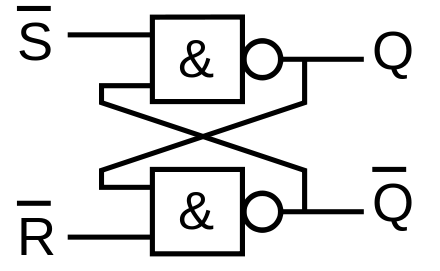
\includegraphics[width=0.60\linewidth]{images/processeurs_porte_bascule_nand.png}
        \caption{Implémentation à partir de portes \textit{NON-ET}}
        \label{pic_processeurs_porte_bascule_nand}
    \end{subfigure}
    ~ %add desired spacing between images, e. g. ~, \quad, \qquad, \hfill etc. 
      %(or a blank line to force the subfigure onto a new line)
    \begin{subfigure}[]{0.48\linewidth}\centering
        
\includegraphics[width=0.60\linewidth]{images/processeurs_porte_bascule_nor.png}
        \caption{Implémentation à partir de portes \textit{NON-OU}}
        \label{pic_processeurs_porte_bascule_nor}
    \end{subfigure}
    \caption{Réalisation d'une bascule à partir de deux types de portes. La bascule maintient son état actuelle tant que les signaux d'entrée ne changent pas}
    \label{fig_processeurs_porte_bascule}
\end{figure}


\subsection{Les mémoires RAM}
%%%%%%%%%%%%%%%%%%%%%%%%%%%%%%%%%%%%%%%%%%%%%%%%%%%%%%%%%%%%%%%%%%%

La mémoire à accès aléatoires ou \textit{Random Acces Memory} (RAM) est une mémoire dont le temps d'accès ne dépend pas de la position de l'information. Contrairement aux disques ou aux bandes magnétiques dont le temps d'accès pouvait varier en fonction de l'emplacement actuel de la tête de lecture et de la prochaine donnée à lire. La RAM est une mémoire volatile, l'information stockée n'est pas persistante lorsque la mémoire n'est plus alimentée. Il y a eu beaucoup d'évolution des différentes technologies RAM depuis leur création. Il en existe différents types, ayant leurs avantages et leurs inconvénients. Dans une plate-forme actuelle, deux types de mémoires RAM sont principalement utilisées: la RAM statique (SRAM, \autoref{pic_processeurs_porte_sram}) et la RAM dynamique (DRAM, \autoref{pic_processeurs_porte_sram}). La raison principale de la présence de deux types de RAM vient de leur différence de coût de production. La SRAM, bien que plus rapide, est aussi beaucoup plus chère. Cette différence de prix s'explique par l'architecture des deux mémoires ((\autoref{fig_processeurs_ram}).


\begin{figure}
    %\centering
    \begin{subfigure}[]{0.48\linewidth}\centering
        
\includegraphics[width=0.60\linewidth]{images/processeurs_porte_sram.png}
        \caption{Mémoire vive statique (SRAM) utilisant 6 transistors}
        \label{pic_processeurs_porte_sram}
    \end{subfigure}
    ~ %add desired spacing between images, e. g. ~, \quad, \qquad, \hfill etc. 
      %(or a blank line to force the subfigure onto a new line)
    \begin{subfigure}[]{0.48\linewidth}\centering
        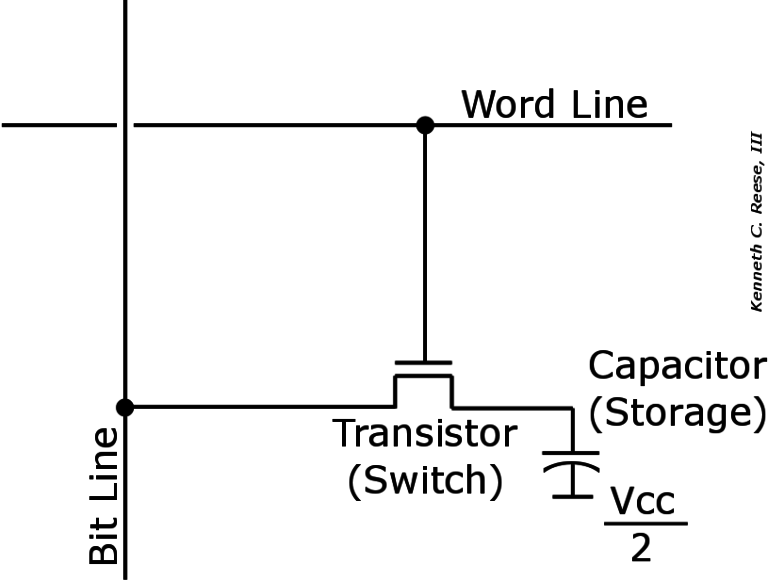
\includegraphics[width=0.60\linewidth]{images/processeurs_porte_dram.png}
        \caption{Mémoire vive dynamique (DRAM) utilisant un condensateur et un transistor}
        \label{pic_processeurs_porte_sram}
    \end{subfigure}
    \caption{Deux types de RAM très utilisées dans les architectures. La différence de complexité de leur circuit électronique explique la différence de prix entre les deux technologies}
    \label{fig_processeurs_ram}
\end{figure}

\subsubsection{La SRAM} 
La RAM statique est un circuit logique qui utilise 6 transistors pour représenter les états 0 et 1 (bien qu'il existe des variantes utilisant 4, 8 ou même 10 transistors). Une SRAM à 6 transistors en utilise 4 pour stocker l'information. Deux transistors additionnels sont utilisés pour contrôler leur accès durant leur lecture ou écriture.
Il est courant d'utiliser différents types de SRAM dans les différents niveaux de caches pour optimiser la densité (mémoire de plus grande capacité) ou la vitesse d'accès. Le premier niveau de cache étant optimisé pour la vitesse d'accès, contrairement aux caches de niveau supérieur de plus grande capacité.


\subsubsection{La DRAM} 
La RAM dynamique a une structure plus simple que la SRAM qui n'est composée que d'un transistor et d'un condensateur. La valeur du bit est déterminée par la charge (positive ou négative) du condensateur. Qu'il soit VRAI ou FAUX, le condensateur doit donc être chargé. 
À cause des fuites (\textit{leakage}) les condensateurs doivent être rafraîchis en permanence. La fréquence de rafraîchissement est de l'ordre de 1\% à 5\% du temps total d'utilisation de la mémoire. C’est cette spécificité qui fait de la DRAM une mémoire très consommatrice en énergie. Grâce à leur faible nombre de transistors, la densité des mémoires DRAM est élevée permettant la construction de mémoire de grande capacité (en GiB). Cependant, la lecture d’une cellule décharge le condensateur, il faut donc, même lors d’une lecture, le recharger.
La charge et la décharge du condensateur n’étant pas instantanés, la DRAM est beaucoup plus lente que la SRAM (une cellule ne pouvant pas être accédée pendant son rafraîchissement).
La quasi-totalité des ordinateurs des 50 dernières années ont une mémoire centrale utilisant de la DRAM.

%Il existe plusieurs types de DRAM: DDR, GDDR, QDR, HBMC, HMC.


\subsubsection{SRAM vs DRAM}

L'avantage de la SRAM est sa rapidité de fonctionnement et sa faible consommation électrique. Contrairement à la DRAM, la SRAM est statique, elle conserve l'information et ne nécessite pas de rafraîchissement périodique pour conserver la donnée enregistrée. Cependant, elle s'efface si aucune tension ne lui est appliquée en continu.
Le principal inconvénient de la SRAM vient de son coût de fabrication ainsi que leur faible densité (due à l'utilisation de 6 transistors)


\begin{table}[]
\begin{tabular}{l|l|l|}
\cline{2-3}
                                       & SRAM     & DRAM             \\ \hline
\multicolumn{1}{|l|}{Prix/bit}         & élevé    & bas              \\ \hline
\multicolumn{1}{|l|}{Vitesse d'accès}  & rapide   & lent             \\ \hline
\multicolumn{1}{|l|}{Latence}          & 0.5-5 ns & 50-70 ns        \\ \hline
\multicolumn{1}{|l|}{Rafraichissement} & non      & oui              \\ \hline
\multicolumn{1}{|l|}{Consommation}     & basse    & élevée           \\ \hline
\multicolumn{1}{|l|}{Énergie/bit}      & n pj     & n pj             \\ \hline
\multicolumn{1}{|l|}{Densité}          & faible (6 transistors par bit)   & élevée (1 transistor par bit)          \\ \hline
\multicolumn{1}{|l|}{Complexité}       & grande   & faible           \\ \hline
\multicolumn{1}{|l|}{Utilisation}      & Cache    & Mémoire centrale \\ \hline
\multicolumn{1}{|l|}{Endurance}        & todo     & $10^{16}$           \\ \hline
\end{tabular}
\end{table}




\subsection{Évolution des transistors}
%%%%%%%%%%%%%%%%%%%%%%%%%%%%%%%%%%%%%%%%%%%%%%%%%%%%%%%%%%%%%%%%%%%


La vitesse de calcul d'un processeur ou la capacité de stockage d'une mémoire sont directement liées au nombre de transistors disponible sur une puce. 
Plus un processeur aura de transistors, au plus il pourra calculer rapidement (ajout de coeur, meilleures unités de calculs). Plus une mémoire aura de transistors, au plus elle pourra contenir de cellule RAM et donc avoir une grande capacité de stockage. La performance des systèmes informatiques est donc directement liée aux technologies de transistors utilisées. 


\subsubsection{Évolution du nombre de transistors.}

L'évolution du nombre de transistors sur une puce a été prédite par l'un des trois fondateurs de la société Intel, Gordon Moore. En 1965, Gordon Moore prévoit que le nombre de transistors d'un puce doublera chaque année, sur une même surface et pour un coût constant \cite{Moore1998}. Il réévaluera cette période à 2 ans en 1975 \cite{Moore75}, ce qui correspond parfaitement avec l'évolution réelle jusqu'à ces dernières années (\autoref{pic_Moore_prediction}).




\begin{figure}
    %\centering
    \begin{subfigure}[]{0.48\linewidth}\centering
        \vspace{1cm}
        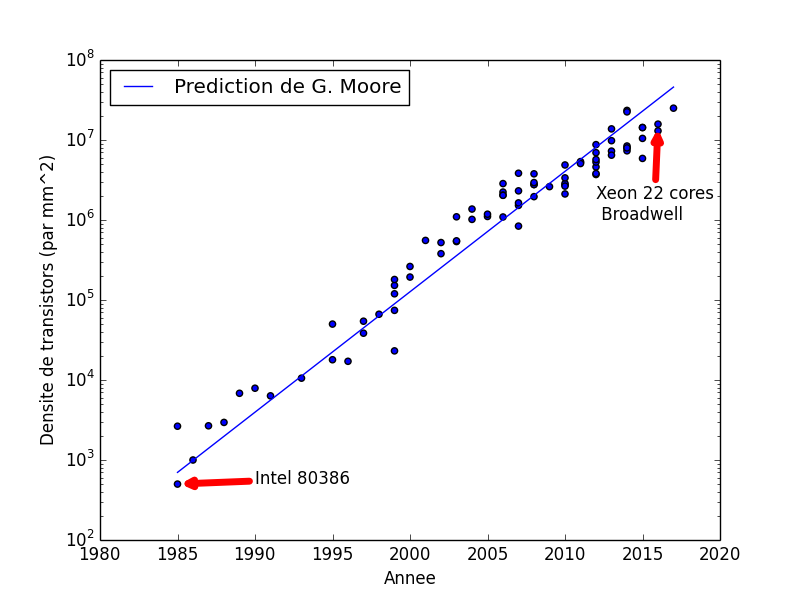
\includegraphics[width=\linewidth]{images/Chapitre1/Moore_prediction.png}
        \caption{\label{pic_Moore_prediction} Évolution du nombre de transistors des processeurs Intel (données \cite{Wikipedia2019Transistor})}
    \end{subfigure}
    ~ %add desired spacing between images, e. g. ~, \quad, \qquad, \hfill etc. 
      %(or a blank line to force the subfigure onto a new line)
    \begin{subfigure}[]{0.48\linewidth}\centering
        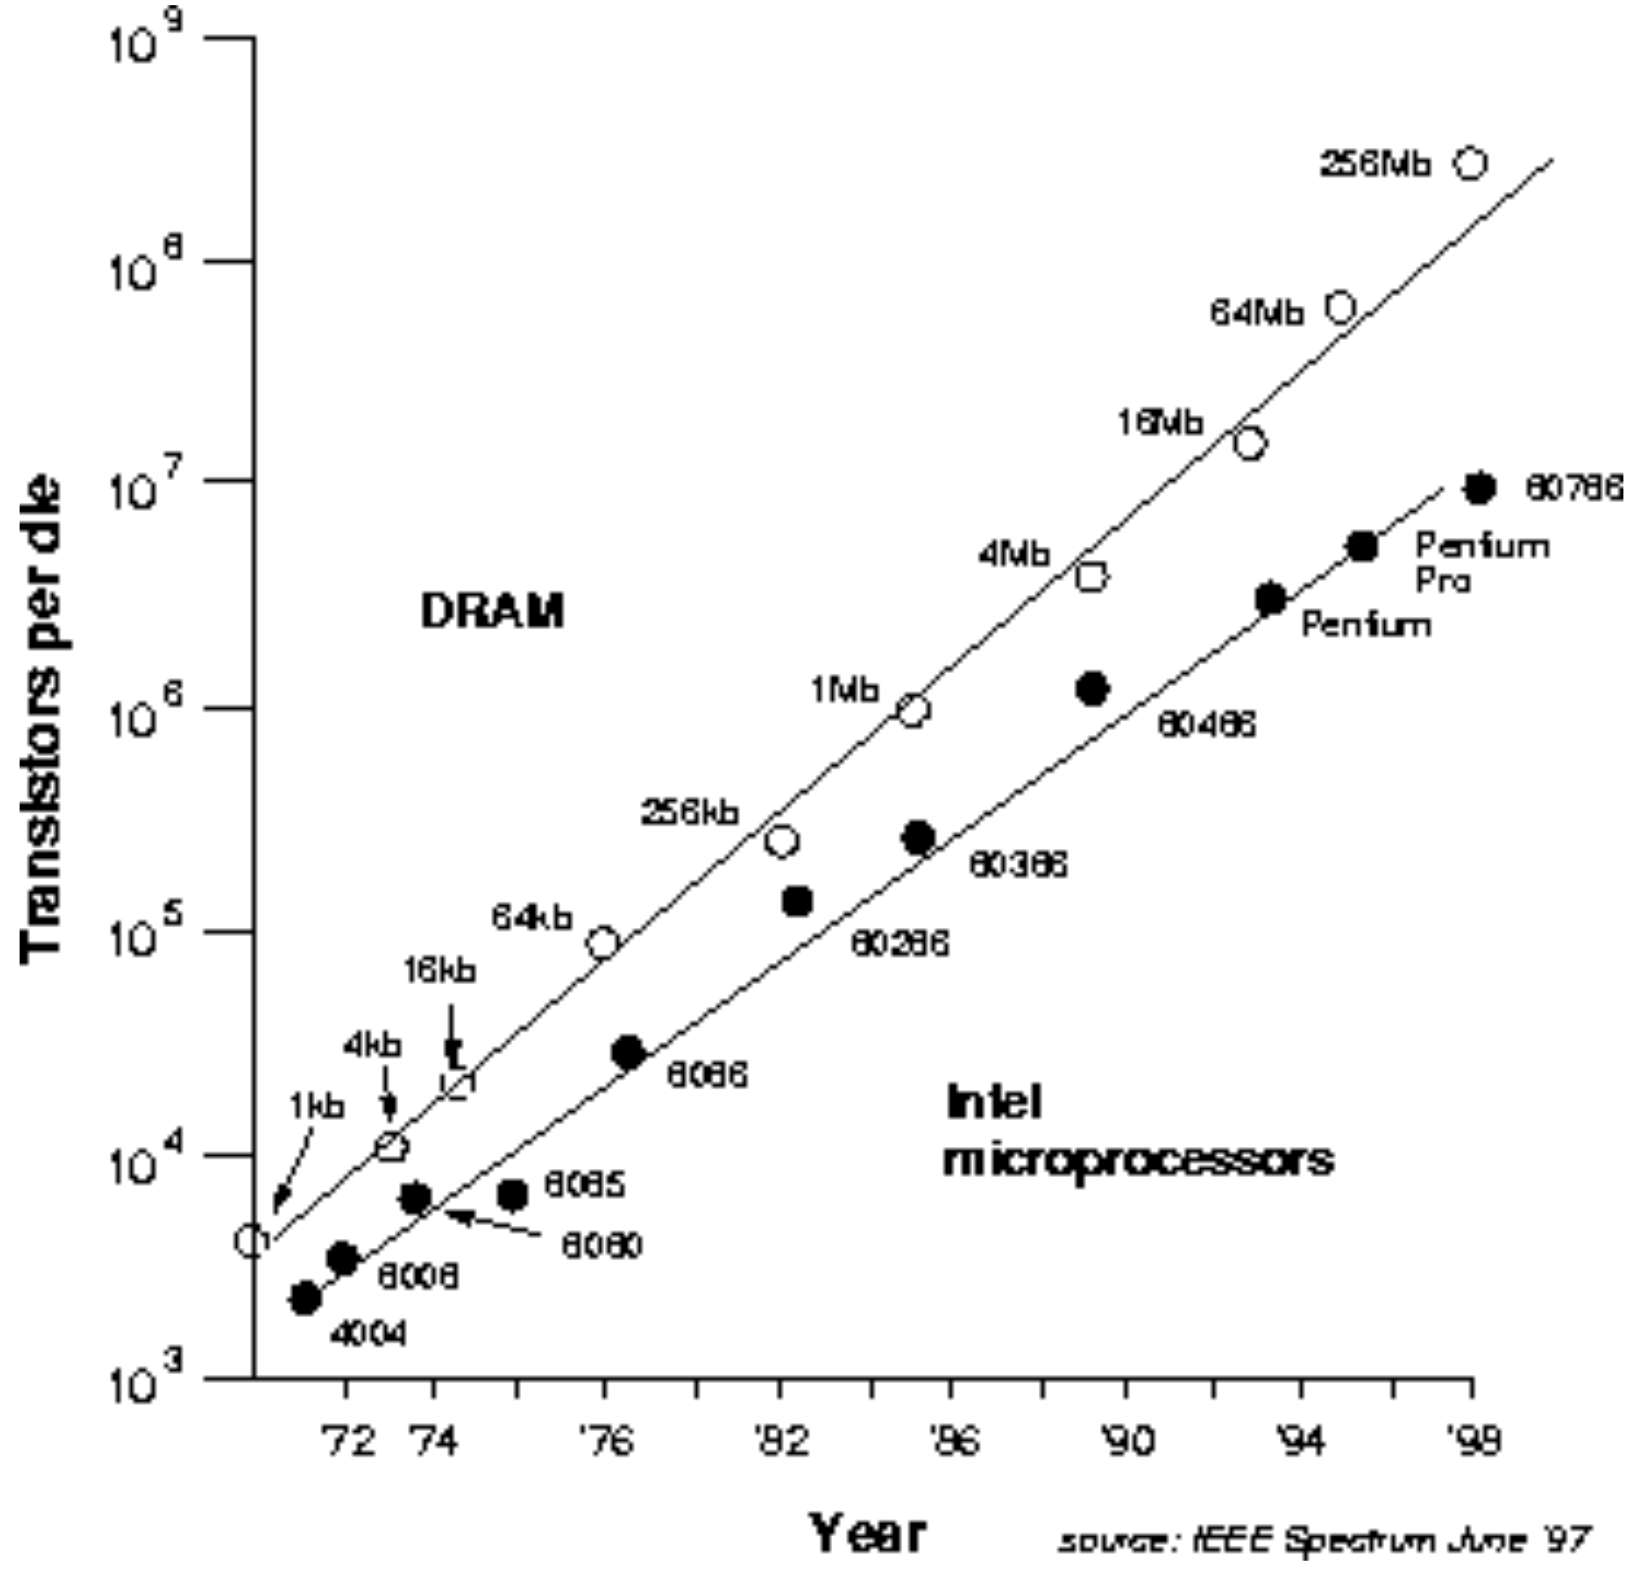
\includegraphics[width=0.9\linewidth]{images/processeurs_porte_moore_dram.png}
        \caption{La loi de Moore s'applique aux processeurs comme aux mémoires DRAM.}
        \label{processeurs_porte_moore_dram}
    \end{subfigure}
    \caption{La loi de Moore décrit l'évolution de la densité de transistors qui double tous les deux ans pour un prix constant.}
    \label{fig_processeurs_moore}
\end{figure}





\subsubsection{Coût de la gravure.}

La notion de coût est souvent oubliée lorsque la loi de Moore est citée. Cependant c'est un aspect fondamental de la loi. Les procédés de fabrication étant plus complexes, les usines de fabrication coûtent elles aussi de plus en plus cher. L'augmentation du coût des fonderies a elle aussi été prédite par la seconde loi de Gordon Moore (loi de Rock), qui estime que leur prix double tous les 4 ans \cite{schaller1997moore}. Bien que les coûts de fabrication augmentent, la taille de gravure s’affine et permet de mettre plus de transistors sur une même surface, permettant ainsi à l’industrie de suivre la cadence dictée par la loi de Moore (\autoref{pic_Moore_explique}).

\begin{figure}
    \center
    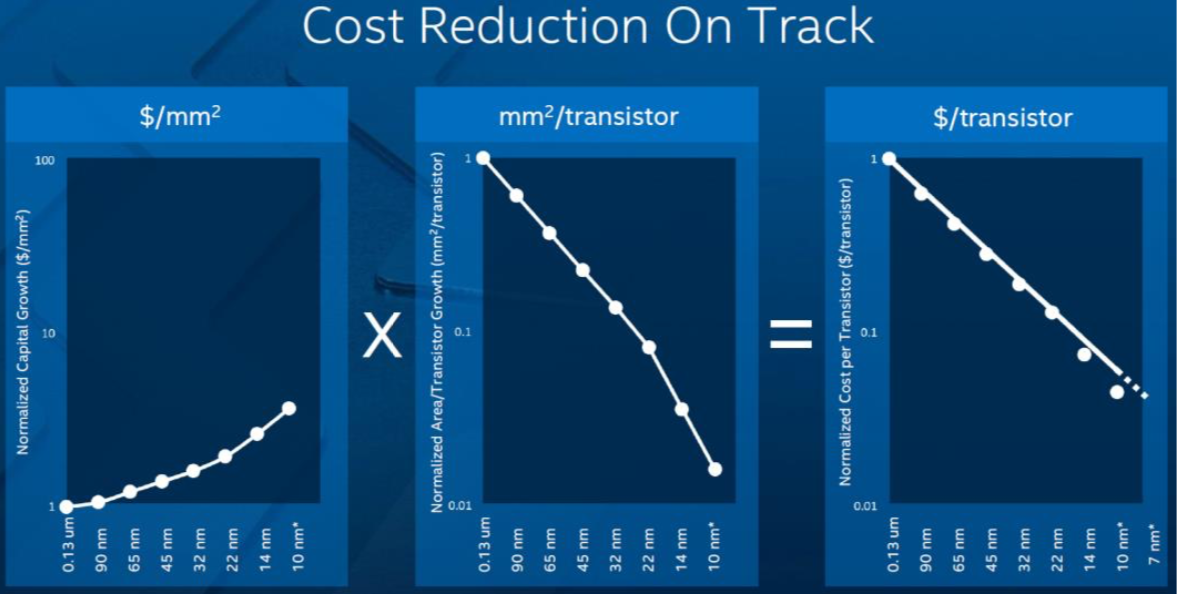
\includegraphics[width=10cm]{images/processeurs_porte_moore.png}
    \caption{\label{pic_Moore_explique} Bien que le prix des fonderie augmente, le nombre de transistors gravable sur une puce augmente plus rapidement. Conséquence de la loi de Moore: le prix par transistor diminue exponentiellement.}
\end{figure}



\subsubsection{Les fondeurs.}
Pour doubler le nombre de transistors sans changer la surface grave, il faut graver des transistors deux fois plus petits. 
Depuis plus de cinquante ans, les \textbf{fondeurs} (les industriels responsable de la gravure des processeurs) tels que Samsung Electronics, TSMC, Intel et GlobalFoundries ont développés de nombreuses techniques et technologies pour réduire la taille des transistors (voir \autoref{processeurs_porte_fondeurs}). Aujourd'hui, de nombreuses étapes sont nécessaire pour transformer une plaque de silicium (la plus pure possible) en processeurs: dopage, déposition d'une couche de résine, gravure, traitement thermique, revêtement par couche mince, découpe, encapsulation... \cite{AnthonyNelzinSantos2018}.
Les procédés de fabrication étant plus complexes, les usines de fabrication coûtent elles aussi de plus en plus cher. L'augmentation du coût des fonderies à lui aussi été prédit par la seconde loi de Gordon Moore (ou \textit{loi de Rock}), qui estime que leur prix double tous les 4 ans \cite{schaller1997moore}.


Cependant, les finesses de gravures atteintes aujourd'hui sont tellement faibles qu'elles atteignent une limite physique, celle de la taille des atomes. A des tailles proches de quelques atomes, les courants électriques ne sont plus stables et la course à la réduction des finesses de gravure n'a jamais été aussi difficile.
Voila plusieurs années, qu'Intel ne parvient plus à descendre sous les 10 nm. Les procédés à mettre en oeuvre pour y parvenir sont si complexes, qu'il est courant de parler de la fin de la loi de Moore \cite{theis2017end}.
En 2019, Samsung annonce qu'il a mis au point une technologie permettant la gravure des premiers processeurs en 3 nm dès 2021 \cite{AdrianBRANCO2019}. 


\begin{figure}
    \center
    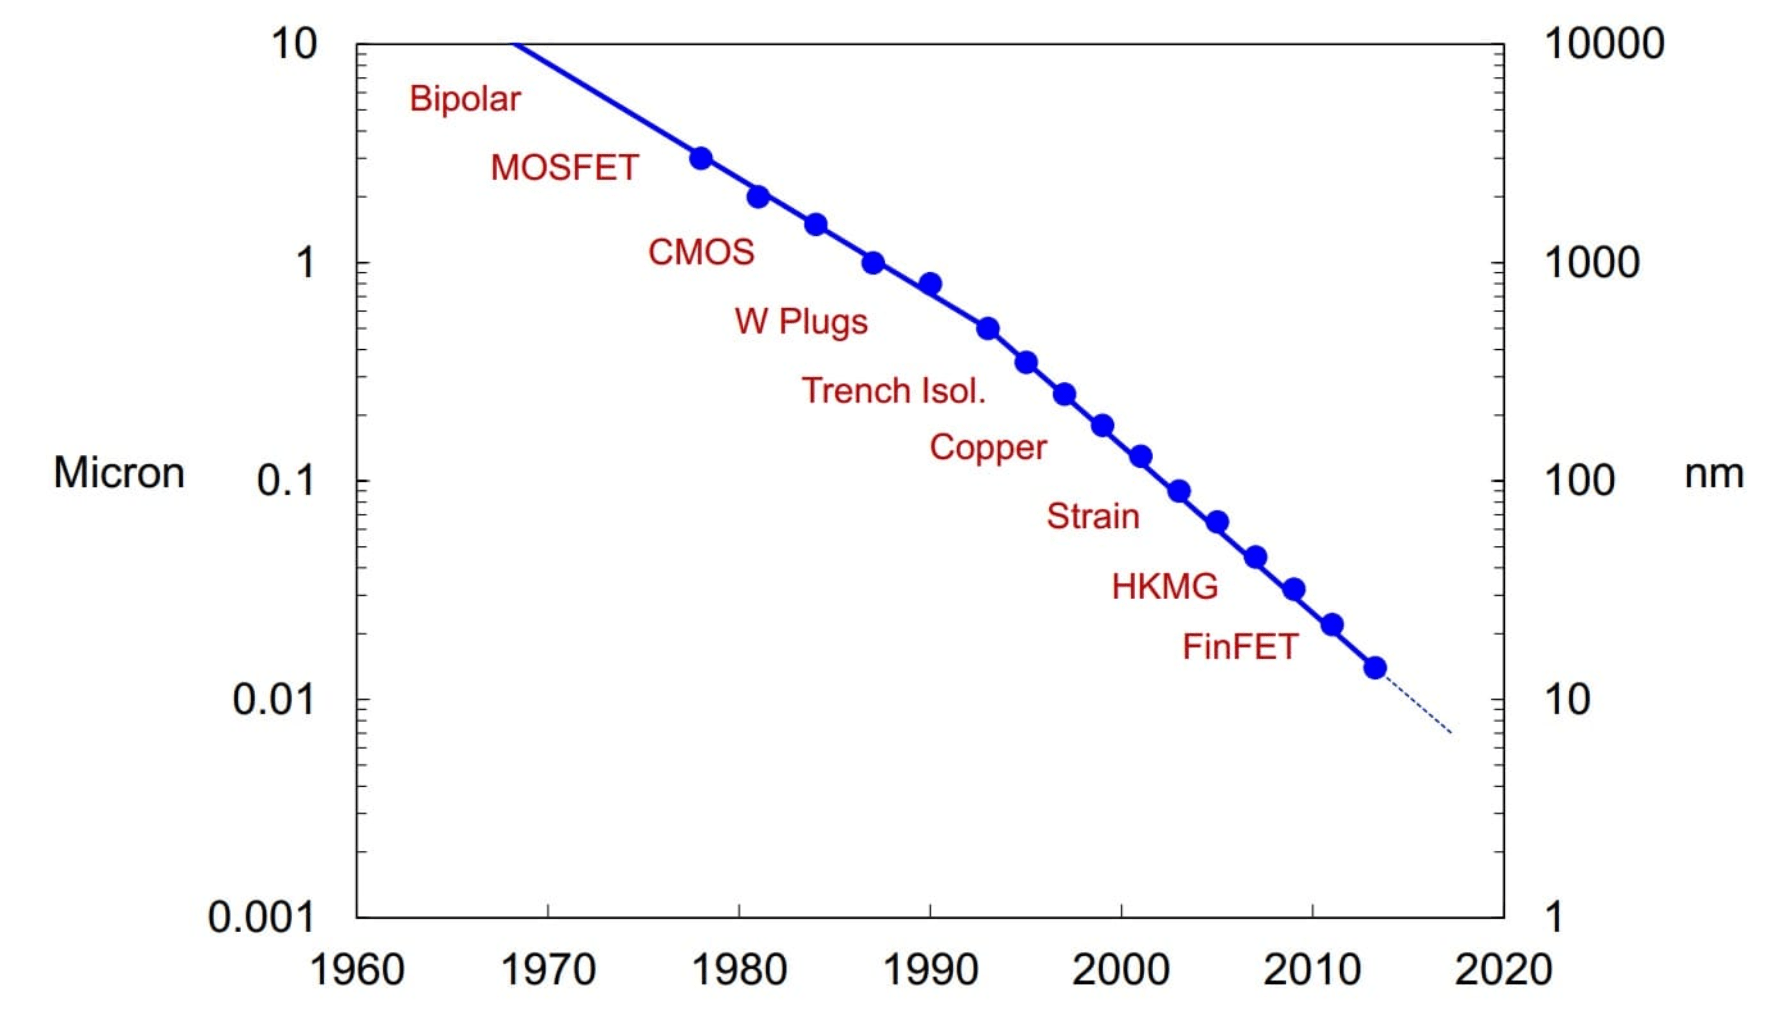
\includegraphics[width=10cm]{images/processeurs_porte_fondeurs.png}
    \caption{\label{processeurs_porte_fondeurs} Les technologies utilisées pour la gravure ont évoluées, rendant les fonderies plus performantes mais aussi plus chères (source Intel).}
\end{figure}












%%%%%%%%%%%%%%%%%%%%%%%%%%%%%%%%%%%%%%%%%%%%%%%%%%%%%%%%%%%%%%%%%%%
%%%%%%%%%%%%%%%%%%%%%%%%%%%%%%%%%%%%%%%%%%%%%%%%%%%%%%%%%%%%%%%%%%%



\section{L'architecture} \label{sec:micro}
%%%%%%%%%%%%%%%%%%%%%%%%%%%%%%%%%%%%%%%%%%%%%%%%%%%%%%%%%%%%%%%%%%%
%%%%%%%%%%%%%%%%%%%%%%%%%%%%%%%%%%%%%%%%%%%%%%%%%%%%%%%%%%%%%%%%%%%

Dans la section \autoref{sec:logique} sont présentés les transistors, les éléments de bases des ordinateurs. Les transistors sont groupés en portes logiques pour construire des circuits électroniques. Cette section présente comment ces circuits sont utilisés pour construire la micro-architecture d'un ordinateur, capable d'exécuter les instructions défini par une \textit{Instruction Set Architecture} (ISA). L'objectif n'est pas de présenter la totalité de l'architecture mais seulement les éléments importants nécessaires pour la suite de la thèse.


Afin d'éviter toutes confusions, nous rappelons la définition de la micro-architecture et de l'ISA car ces termes sont souvent confondus dans la littérature:

\begin{itemize}
    \item  \textbf{La couche ISA} (\textit{Instruction Set Architecture}) regroupe les instructions, leur mode (système ou utilisateur), les registres utilisables, l'organisation du système mémoire (alignement, espace d'adressage) ... 
    C'est une spécification formelle établie, qui peut être utilisée par plusieurs fabricants de micro-architecture \cite{tanenbaum2016structured}. Intel publie fréquemment la documentation de l'ISA x86 \cite{guide2011intel}. Elle forme l'interface entre le matériel et le logiciel et permet la compatibilité de programme sur des micro-architectures de différents constructeurs. 
    Grâce à la couche ISA, différents langages de programmation peuvent être utilisés pour écrire les application. Le compilateur s'occupe alors de les traduire dans un langage bas niveau pouvant utiliser l'ISA (langage assembleur). Ce langage est tellement proche de la couche ISA que les deux termes sont souvent mélangés. Les \textit{ISA} existantes sont listées dans la \autoref{sec:isa}. 

    \item \textbf{La micro-architecture} correspond à l'implémentation matériel de l'\textit{ISA} est implémentée matériellement par la micro-architecture. Ce sont deux couches distinctes, la seconde n'ayant pas forcément besoin d'avoir connaissance de la première (bien que pour des raisons de performances cela soit préférable). En ayant connaissance de la micro-architecture, le compilateur pourra réordonner ou modifier des instructions pour tirer parti du pipeline ou d'un processeur vectoriel. La conception d'une nouvelle micro-architecture doit commencer par choisir l'ISA à implémenter (si possible existante pour permettre la compatibilité des programmes). Les différences principales entre deux micro-architectures implémentant la même ISA sont leur différence de performances et de coût. Les processeurs Intel et AMD implémente la même \textit{ISA x86}. La performance et le nombre d'instructions supportés par les deux architectures est cependant différent.
    
    \item Le terme d'\textbf{architecture} est souvent employé à la place du terme \textit{ISA}, notamment par IBM en 1964 \cite{amdahl1964architecture}.  Aujourd'hui il est souvent utilisé pour faire référence à la fois à l'\textit{ISA} et à la \textit{micro-architecture}. Il est courant d'entendre parler d'\textit{architecture x86} pour faire référence à une micro-architecture implémentant l'\textit{ISA x86}.\\ 
\end{itemize}



\subsection{Performance d'une architecture}
%%%%%%%%%%%%%%%%%%%%%%%%%%%%%%%%%%%%%%%%%%%%%%%%%%%%%%%%%%%%%%%%%%%


Le développement d'une nouvelle micro-architecture doit prendre en compte plusieurs facteurs qui peuvent impacter son implémentation (vitesse de traitement des instructions, le coût de fabrication, la fiabilité, consommation électrique, taille). Ces différents facteurs font pression sur les architectes de processeurs qui doivent redoubler d'inventivité pour les satisfaire en implémentant des optimisation matériels.

Les améliorations ont pour but d'améliorer la performance de l'architecture, la plus part du temps de façon transparente pour l'utilisateur. Cependant, un programmeur n'étant pas avertis de ces optimisations, pourrait écrire des applications inefficaces voire contre-productive. Les développeurs d'applications \textit{HPC} étant généralement des scientifiques experts dans leur domaine (physique, chimie, mécanique…), il est fréquent de voir des codes peu efficaces. Cette section, liste les principales améliorations des micro-architectures qu'il faut connaître et utiliser pour exploiter le maximum des performances disponibles. 


Pour améliorer la vitesses d'exécution d'un programme, quatre moyens peuvent être utilisés:
\begin{itemize}
    \item Utiliser une nouvelle technologie, plus rapide, consommant moins d'énergie, moins cher ou plus dense (technologie mémoire, fibre optique...). Les nouvelles technologies sont nombreuses et les principales sont listées et discutées dans la \autoref{sec:opportunité}. 
    \item Améliorer l'efficacité des instructions: \autoref{sec:efficacite} 
    \item Accélérer l'exécution des instructions: \autoref{sec:accelerer}
    \item Exécuter les instructions en parallèle: \autoref{sec:para}
\end{itemize}

Quand elles ne sont pas matérielles, ces différentes améliorations peuvent être réalisés par deux techniques: dynamique ou statique. Les méthodes statiques interviennent avant que le code soit exécuté. Généralement, c'est le compilateur qui les implémente lors de la génération du code. Les techniques dynamiques sont mis en oeuvre au fil des exécutions d'instructions. Elles nécessitent donc du matériel spécialisé supplémentaire et sont donc très coûteuses. La section présente les principales techniques et matériels utilisés pour l'amélioration des performances (dynamique et statique). Deux améliorations majeures sont présentées dans deux section distinctes: la hiérarchie mémoire (\autoref{sec:hierarchie} et la mémoire virtuelle (\autoref{sec:memoire_virtuelle}).







%%%%%%%%%%%%%%%%%%%%%%%%%%%%%%%%%%%%%%%%%%%%%%%%%%%%%%%%%%%%%%%%%%%
\subsection{Améliorer l'efficacité de l'exécution} \label{sec:efficacite}
%%%%%%%%%%%%%%%%%%%%%%%%%%%%%%%%%%%%%%%%%%%%%%%%%%%%%%%%%%%%%%%%%%%




\subsubsection{Jeu d'instructions ISA } \label{sec:isa}
%%%%%%%%%%%%%%%%%%%%%%%%%%%%%%%%%%%%%%%%%%%%%%%%%%%%%%%%%%%%%%%%%%%

Le choix de l'\textit{ISA} à implémenter est le premier choix à réaliser lors du développement d'une nouvelle micro-architecture. L'\textit{ISA} utilisée à un impact sur la performance, la facilité de programmation, les applications compatibles...

Les jeux de d'instructions existant sont séparés en deux grandes familles d'ISA: les jeux d'instructions CICS pour \textit{Complex Instruction Set Computing} et les instructions RISC pour \textit{Reduced Instruction Set Computing}. La principale différence entre les deux est la complexité de leurs instructions. 

    \paragraph{CISC} est la première famille d'instructions à avoir été utilisé massivement. Ces instructions sont dites complexes car une seule instructions peut à elle seule demander plusieurs opérations à réaliser. Par exemple une addition CISC s'occuperait de charger les données depuis la mémoire, d'exécuter l'addition ensuite et sauver le résultat. A l'origine, beaucoup de codes étaient écrit en assembleur, et ce genre d'instructions permettaient au programmeur d'éviter d'écrire de nombreuses lignes de codes souvent redondantes. De plus les codes générés en CISC sont plus petit et nécessitent donc moins de mémoire, qui à l'origine manquait énormément.

    \paragraph{RISC} regroupe les ISA dites \textit{simple}. En 1970, John Cocke, alors ingénieur chez IBM, proposa de réduire le nombre d'instructions CISC \cite{cocke1990evolution}. Le terme \textit{réduit} fait référence au nombre d'instructions plus petit que celles de CISC mais aussi pour signifier que le travail à réaliser par une instructions était moindre que pour une instruction CISC. Pour réaliser une multiplications entre deux données, on devra alors explicitement charger la première donnée, puis la deuxième et enfin écrire l'instruction qui correspond à la multiplication. Les instructions étant plus nombreuses le travail des compilateurs est augmenté mais souvent l'exécution des codes résultantes en est réduite. Le RISC fut une réponse apporté a la lenteur de décodage du CISC.  Toutes les instructions font la même taille, les architectures nécessitent donc moins de transistors pour les analyser. Les micro-architecture sont donc moins coûteuses et peuvent atteindre des fréquences plus élevées.

Ces deux familles d'instructions ont toutes deux leurs avantages et leurs inconvénients et les puces actuelles comportent des parties qui exécutent des instructions RISC et d'autres en CISC. L'ISA la plus rependu est le x86 qui se veut être un jeu d'instruction CISC. Le RISC augmente le nombre d'instructions lues séparément par le micro-processeur, si cela à le désavantage de consommer plus de mémoire, cela à aussi d'autre avantages, comme de pouvoir optimiser leur exécution avec la mise en place d'un \textit{pipeline}. Les \textit{ISA RISC} les plus connus sont les \textit{ISA} ARM, \textit{MIPS} (utilisé dans le domaine universitaire pour apprendre le langage assembleur), PA-RISC (Hewlett-Packard) et RISC-V. L'\textit{ISA CISC} la plus utilisée dans les super-calculateurs aujourd'hui est \textit{x86} (processeurs Intel et AMD).



\paragraph{Extensions vectorielles}.
Pour tirer partie de la puissance de calculs des processeurs et des unités de calculs vectorielles, les \textit{ISA} ont reçu de nombreuses extensions (\autoref{tab_simd}).
C'est en 1995 que Sun Microsystem introduit son premier jeu d'instruction vectoriel, le Visual Instruction Set auquel Intel répondra en 1997 avec son processeur Pentium MMX et le jeu d'instructions du même nom. Ainsi ces instructions pouvaient réaliser des opérations sur les jeux de données tel que les images ou vidéos de facon tres performante. En 1997 AMD viendra ameliorer le jeu d'instruction MMX avec l'implémentions des instructions 3DNow ! qui rendait alors possible les operations vectoriels sur les nombre flottant. La possibilite de faire une operation sur deux nombre flottant par cycle doublait alors la performance des processeurs. Intel repondit alors a cette avance avec le jeu d'instructions Streaming SIMD Extensions (SSE) en 1999. Il est alors facile d'augmenter la puissance des processeurs : il suffit d'augmenter la taille des vecteurs.
L'\textit{ISA x86} reu plus de dix extensions dans les vingts dernires annes pour s'adapter l'agrandissement des units vectorielles. Les principales sont \textit{MMX} (1996), \textit{3DNOW!} (1998), 6 versions de \textit{SSE} de 1999 2008 et enfin \textit{AVX-2} et \textit{AVX-512} en 2013 et 2015. videmment, les codes ne peuvent pas profiter de ces instructions sans une micro-architecture capable de les excuter. Ces micro-architectures sont prsentes dans la sous-section suivante. 


\begin{table}[]
\centering
\caption{Évolutions principales des instructions SIMD $x86$}
\label{tab_simd}
\begin{tabular}{|l|l|l|l|l|l|}
\hline
\multicolumn{1}{|c|}{\textbf{Année}} & \multicolumn{1}{c|}{\textbf{Nom}} & \multicolumn{1}{c|}{\textbf{Nb registres}} & \multicolumn{1}{c|}{\textbf{Taille (bit)}} & \multicolumn{1}{c|}{\textbf{Registres}} & \multicolumn{1}{c|}{\textbf{Commentaires}} \\ \hline
1996                                 & MMX                               & 8                                          & 64                                         & MM0                                     & Nombre entiers
\\ \hline
1999                                 & SSE                               & 8                                          & 128                                        & XMM0                                    & 120 instr., simple precisions              \\ \hline
2006                                 & SSSE3                             & 8                                          & 128                                        & XMM0                                    & 300 instr., double précisions              \\ \hline
2008                                 & AVX                               & 16                                         & 128                                        & XMM0                                    & FMA4, op. a 3 opérandes                    \\ \hline
2011                                 & AVX2                              &  16                                          & 256                                        & YMM0                                    &                                            \\ \hline
2013                                 & AVX512                            & 32                                         & 512                                        & ZMM                                     & FMA3                                       \\ \hline
\end{tabular}
\end{table}

\begin{figure}
    \center
    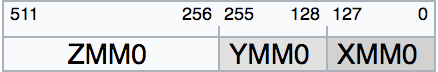
\includegraphics[width=7cm]{images/Chapitre1/simd_registres.png}
    \caption{\label{pic_simd_registres} Découpage d'un registre de 512 bits}
\end{figure}

\subsubsection{Les processeurs vectoriels } \label{sec:cpu_vectoriel}
%%%%%%%%%%%%%%%%%%%%%%%%%%%%%%%%%%%%%%%%%%%%%%%%%%%%%%%%%%%%%%%%%%%

Dans les années 90, les ordinateurs personnels commençaient à être utilisés pour le multimédia (film, image, musique). Dans le but d'augmenter la performance des applications les architectes ont voulu améliorer l'efficacité des instructions en implémentant des architectures SIMD (Single Instruction Multiple Data de la taxonomie de Flynn ). 


L'architecture vectorielle repose sur les même fondement que l'architecture superscalaire: réduire le temps d'exécution d'un code en utilisant le parallélisme et diminuer le coût en transistors de la micro-architecture par la mise en commun du matériel entre plusieurs unités de calculs (\autoref{pic_cpu_simd}). La pression que subit l'unité responsable du \textit{fetch} et du \textit{decode} est donc réduire car avec une seule instruction vectorielle, le processeur réalise le travaille de plusieurs instructions scalaires.  Contrairement au processeur scalaire qui exécutent une instructions sur une seule donnée, les processeurs vectoriels sont capables d'exécuter une instructions sur plusieurs données simultanément (\autoref{pic_simd2}).


Il en résulte que doubler largeur des instructions revient à doubler le nombre de FLOP réalisable par le processeur alors que la consommation électrique augmentera d'un facteur inférieur à 2. Beaucoup d'efforts ont donc été réalisé pour être capable d'utiliser cette technologie, par exemple la majorité des compilateurs est capable de détecter les zones de codes parallélisable pouvant bénéficier d'instructions SIMD.

Cependant, dans la pratique les codes ne sont pas aussi parallèle que nous le souhaiterions et certains aspect du code empêche de tirer la totalité de la performance disponible. En effet, si les données sont indépendantes les unes des autres, il est alors impossible de les calculer simultanément rendant la partie vectorielle inutilisable. Aussi, les performances peuvent être réduites si les données accédées ne sont pas continues en mémoire. Cela demande donc un travail supplémentaire pour repenser les structures de données et s'assurer que les donnes transférées sur le bus mémoire sont des données utiles (voir le concept de ligne de cache dans la \autoref{sec:cache}).

\begin{figure}
    \begin{subfigure}[]{0.5\linewidth}\centering
        \vspace{1.6cm}
        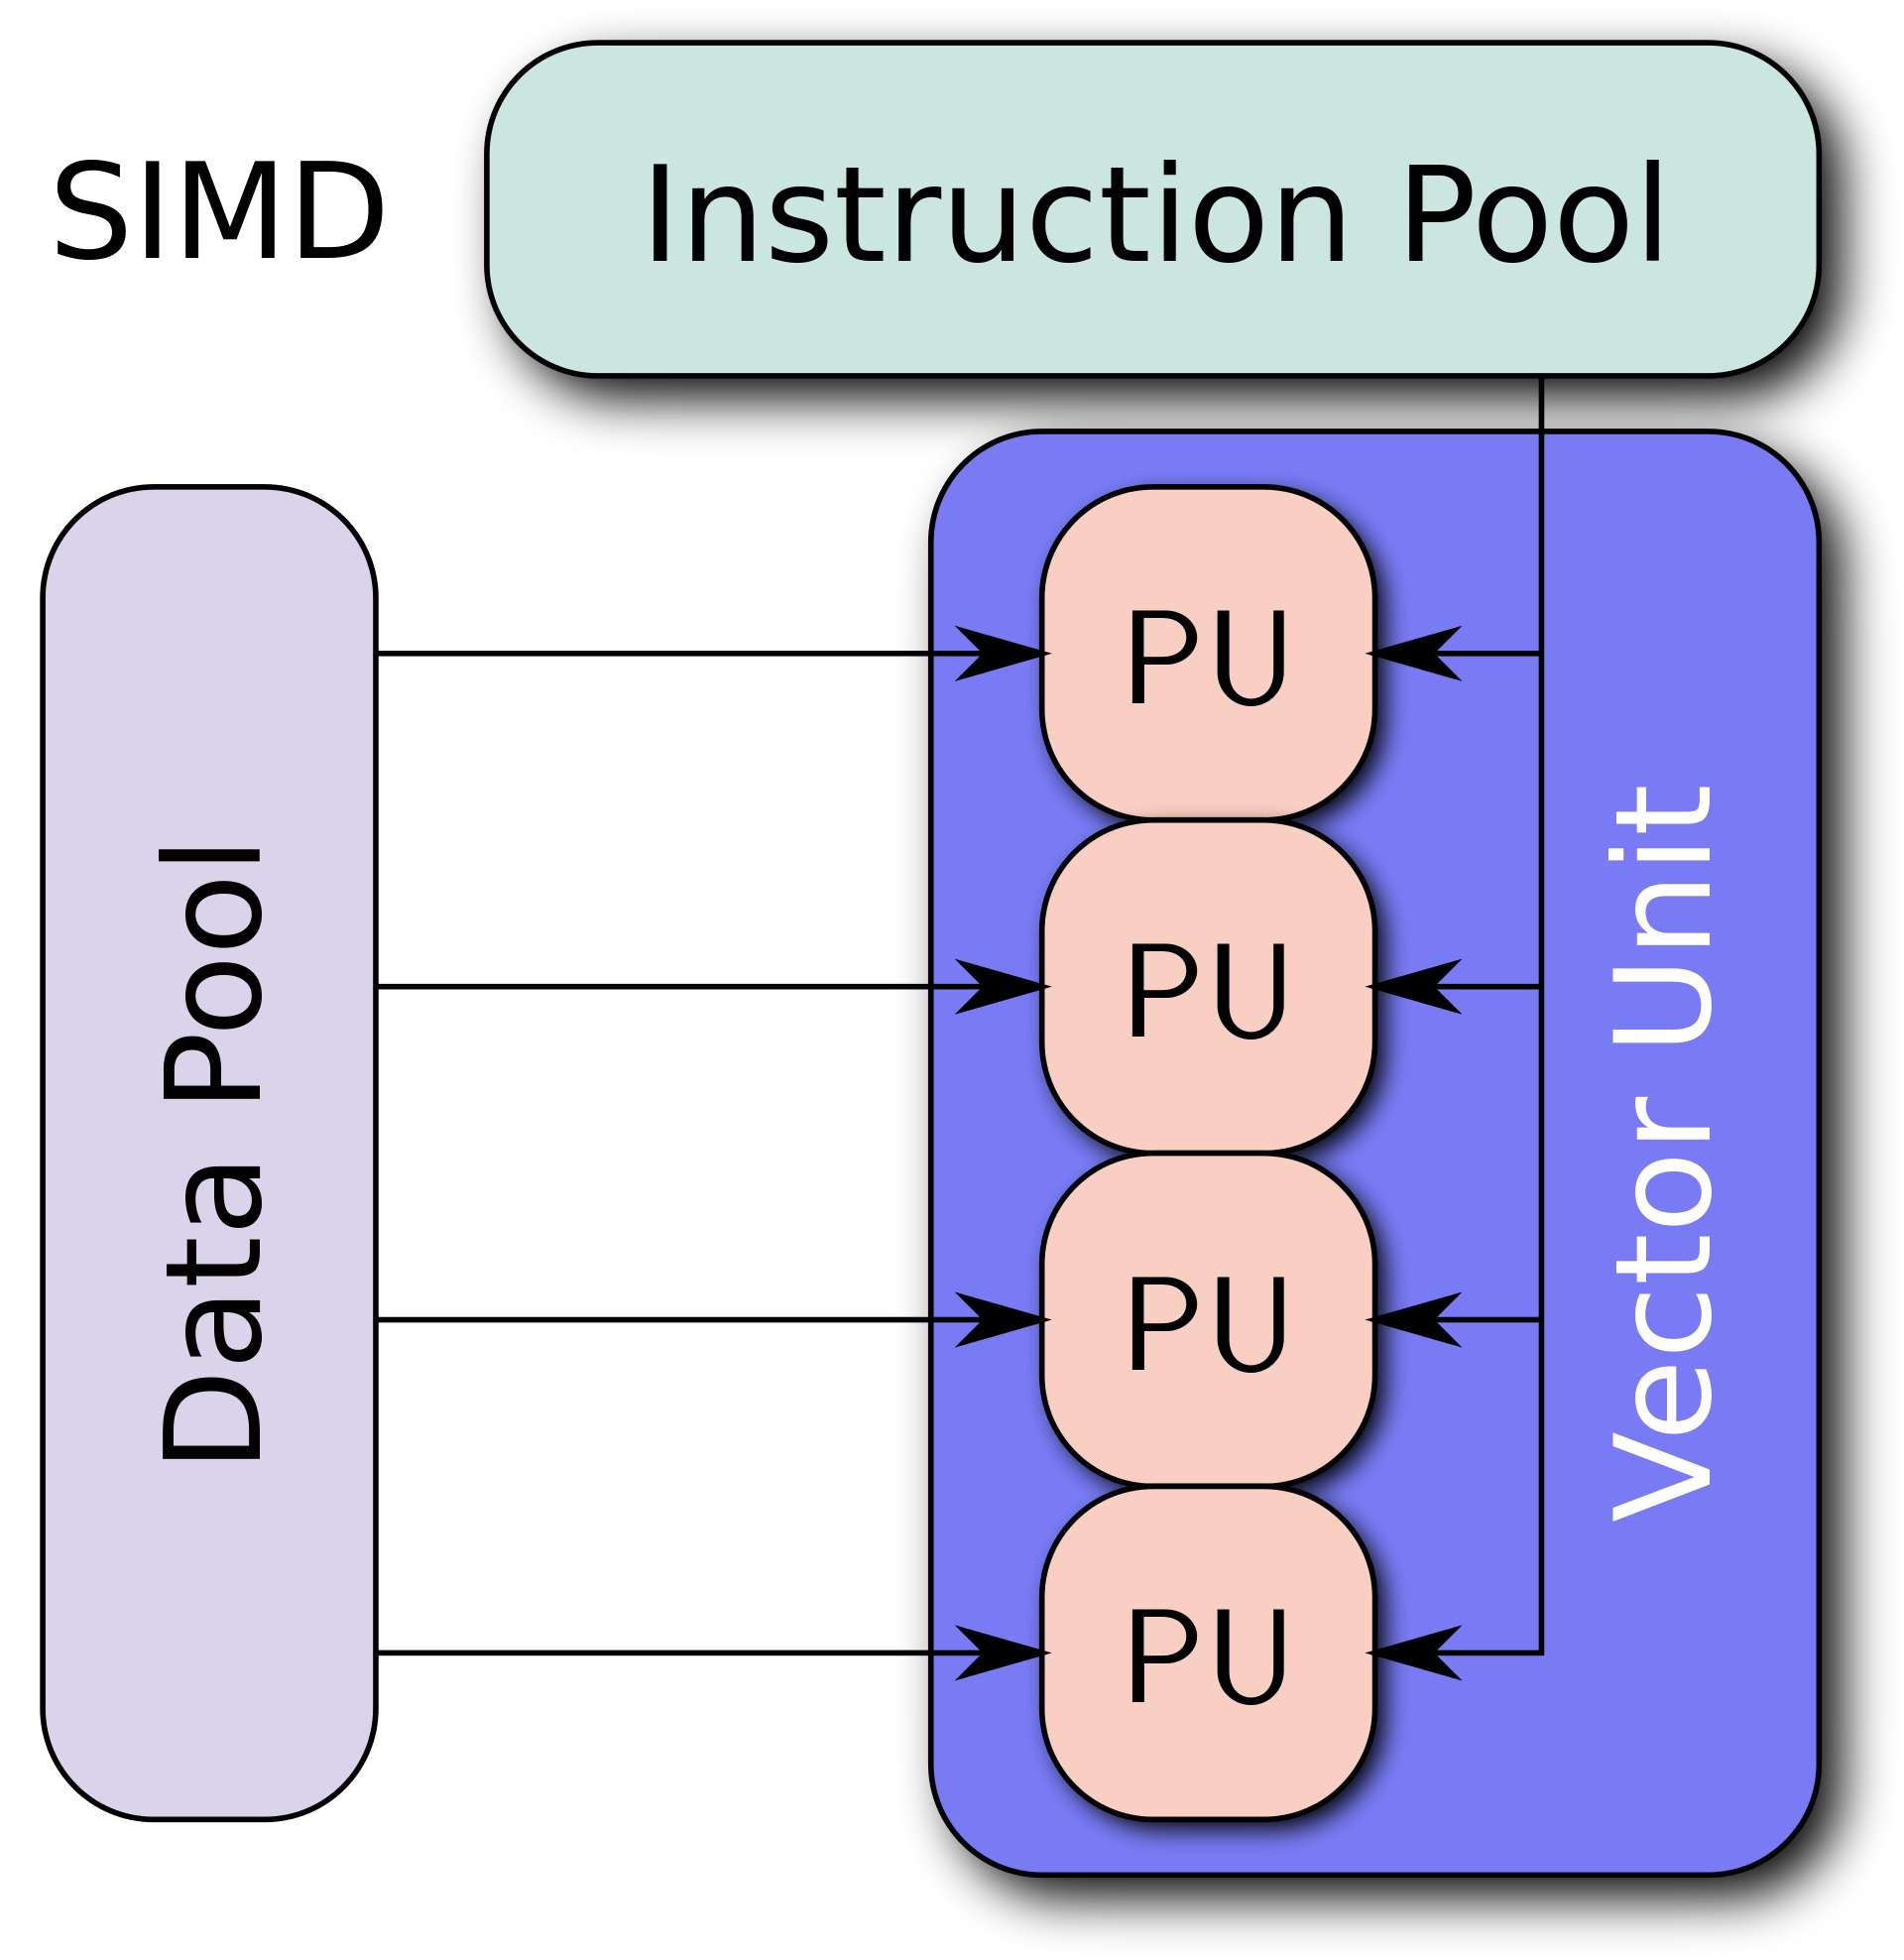
\includegraphics[width=.5\linewidth]{images/cpu_simd.png}
        \label{pic_cpu_simd}
        \caption{Un processeur vectoriel exécute une même instruction sur différentes données}
    \end{subfigure}%
    ~ %space
    \begin{subfigure}[]{0.5\linewidth}\centering
        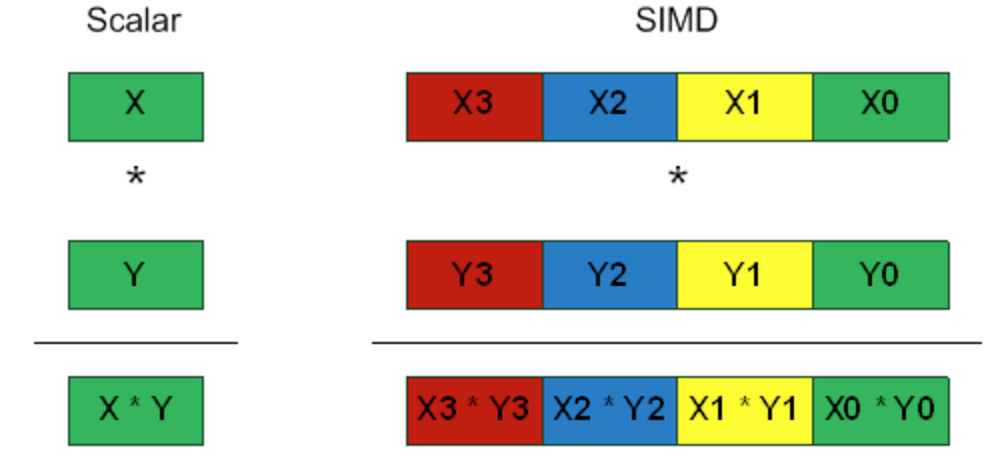
\includegraphics[width=\linewidth]{images/Chapitre1/simd.png}
        \caption{Schéma de fonctionnement d'une multiplication vectorielle\protect\footnotemark}
        \label{pic_simd2}
    \end{subfigure}
   
    \caption{Un processeur vectoriel travaille sur un groupe de données indépendantes. Les opérandes sont alors stockées dans des registres vectoriels capable de charger un vecteur pour y appliquer une même opération.}
    \label{pic_simd}
\end{figure}
\footnotetext{source:\url{https://software.intel.com/en-us/articles/ticker-tape-part-2}}


%%%%%%%%%%%%%%%%%%%%%%%%%%%%%%%%%%%%%%%%%%%%%%%%%%%%%%%%%%%%%%%%%%%
\subsection{Accélérer l'exécution des instructions} \label{sec:accelerer}
%%%%%%%%%%%%%%%%%%%%%%%%%%%%%%%%%%%%%%%%%%%%%%%%%%%%%%%%%%%%%%%%%%%


\subsubsection{Lien entre fréquence et performance}
Les processeurs sont des circuits électronique dits \textit{synchrone}. Leur fonctionnement est cadencé par une horloge donnant des impulsions régulières aux composants du circuit pour organiser leur synchronisation. Lorsqu'une instruction est exécutée par le processeur les passages dans les différentes étapes de la micro-architecture et notamment du pipeline sont régis par cette horloge. Au plus l'horloge est rapide, au plus l'exécution l'est aussi. Cependant, la durée séparant deux signaux (un cycle) ne peut pas être réduite autant que tout architecte le souhaiterait. En effet, les vitesses d'horloges sont si rapide, qu'il est nécessaire de laisser suffisamment de temps au signal électrique de se propager dans le circuit. La taille du processeur et sa fréquence sont donc liées, c'est notamment pour cette raison qu'il n'existe pas de processeur mesurant plusieurs dizaines de centimètres. À une fréquence de 3 GHz, le signal électrique, qui se déplace à la vitesse de la lumière, ne peut parcourir que 15 centimètres entre deux cycles. Au temps de propagation il faut aussi prévoir le temps de préparer et recevoir la communication. L'augmentation de la fréquence des processeurs à donc une première limite physique infranchissable bien que d'autres limites présentées dans cette partie soient encore plus contraignantes.

La fréquence des processeurs a beaucoup évoluée depuis les premiers processeurs (\autoref{pic_cpu_frequency}). Les premiers processeurs \textit{Pentium} d'Intel utilisaient des fréquences de 60 MHz en 1993. Pendant plus de dix ans, les fréquences ont évoluées chaque année d'un facteur de 40\%  \textbf{tous les deux ans ou un ans ???}pour atteindre des vitesses de plusieurs Gigahertz. En 2000, Intel annonçait la fabrication de processeurs cadencés à 10 GHz\footnote{source \url{https://www.clubic.com/actualite-1791-des-processeurs-intel-10-ghz-pour-2005.html}} pour les années 2005. Pourtant, en 2019, nous sommes encore loin d’utiliser des processeurs avec de telles cadences. Mise à part les systèmes surcadencés, utilisant des système de refroidissement liquide, il est rare de voir des systèmes utiliser des processeurs récents à plus de 5 Ghz.

\begin{figure}
    \center
    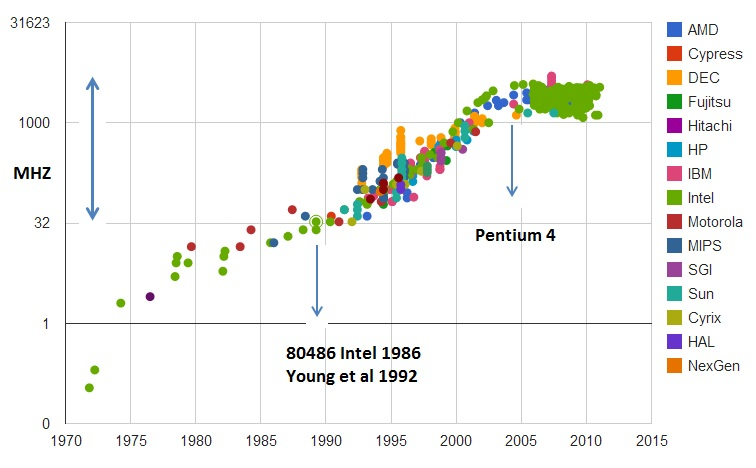
\includegraphics[width=10cm]{images/cpu_frequency.jpg}
    \caption{\label{pic_cpu_frequency} Évolution de la fréquence des processeurs\protect\footnotemark.}
\end{figure}
\footnotetext{source: \url{https://en.wikipedia.org/wiki/Beyond_CMOS}}

Le but de cette section est comprendre pourquoi l'évolution de la fréquence des processeurs s'est arrêtée brusquement autour des 4 GHz. Pour cela, nous expliquons comment la loi de Moore a permis d'en arriver là, et quelles sont les limites physiques qui empêchent de poursuivre cette évolution.

\subsubsection{Loi de Dennard}
Comme constaté dans la section précédente, la fréquence de l'horloge d'un processeur est limitée par le temps nécessaire au signal de se propager entre deux éléments d'un circuit. Au plus les transistors seront proches, au plus la vitesse de propagation sera faible. La loi de Moore prévoit que le nombre de transistors double tout les deux ans pour une surface donnée. Cela est rendu possible par l'affinement de la gravure permettant de réaliser des transistors toujours plus petits et donc plus proches. Avec plus de transistors, les processeurs peuvent utiliser des pipelines plus complexes, entre divisant les étapes les plus longues permettant aussi l'utilisation de fréquence plus élevée. Nous expliquons comment l'évolution de la fréquence des processeurs est intimement liée avec la loi de Moore en utilisant la formule de la consommation électrique d'un circuit CMOS \cite{martin2014post}:
\begin{equation}
P = QfCV^{2} +  VI_{leakage}
\label{eq:power}
\end{equation}

L'intérêt de cette formule est d'apprécier comment la puissance et la fréquence d'un processeur est impactée par la loi de Moore. Pour cela, nous étudions sa variation entre deux générations de processeurs, c'est à dire une période de deux ans.

\paragraph{Le nombre de transistors $Q$.} D'après la loi de Moore, le nombre de transistors double tous les deux ans pour un circuit de même surface. Ainsi la surface des transistors est divisée par deux. Leurs longueur et largeur est ainsi réduite d'un facteur $\sqrt{2}$. Cette valeur est appelé facteur de \textit{scaling} et a une valeur de $1.44$.

\paragraph{La capacité du circuit $C$.} La capacité d'un transistor peut être calculée par la formule suivante $C = \frac{S \times e}{d}$. Avec $S$ la surface du transistor, $e$ la permitivité électrique du matériau utilisé (pouvant être considéré comme fixe entre deux générations), et $d$ la distance séparant la grille et le semi-conducteur (isolant). Comme vu précédemment, la surface $S$ d'un transistor est divisé par $2$ entre deux générations. La distance $d$ est elle réduite par un facteur $\sqrt{2}$. Tous les deux ans, la capacité d'un transistor est donc réduite de $\sqrt{2}$. 

\paragraph{La fréquence du circuit $f$.} La fréquence d'utilisation d'un transistor dépend essentiellement de la vitesse à laquelle la grille peut être chargée ou déchargée. Diminuer sa capacité diminue du même facteur ce temps de remplissage. Entre deux générations, la fréquence est supposée augmenter d'un facteur $\sqrt{2}$. Cette valeur correspond bien à l'augmentation de $40\%$ constatée dans l'introduction de cette section. 

\paragraph{La tension de fonctionnement $V$.} La tension est proportionnelle à la finesse de grave utilisée. Diviser la finesse de gravure pas un coefficient de $\sqrt{2}$ rien à diviser la tension de fonctionnement par le même facteur. 

\paragraph{Les courants de fuites $I_{leakage}$.} Les courants de fuites sont considérés comme négligeables (pour le moment). 

\paragraph{Variation de $P$.} A une tension de fonctionnement $V$ égale entre deux générations de processeurs et en reprenant les variations des différentes valeurs, nous constatons que $P$ ne varie pas entre deux générations. La baisse de capacité compenser l'augmentation de la fréquence (facteur $\sqrt{2}$). La baisse de V NTM 


% Please add the following required packages to your document preamble:
% \usepackage{graphicx}
% \usepackage[table,xcdraw]{xcolor}
% If you use beamer only pass "xcolor=table" option, i.e. \documentclass[xcolor=table]{beamer}
\begin{table}[]
\centering
\resizebox{\textwidth}{!}{%
\begin{tabular}{lc}
\hline
\rowcolor[HTML]{EFEFEF} 
{\color[HTML]{000000} Paramètre} & {\color[HTML]{000000} Coefficient multiplicateur (tous les deux ans)} \\ \hline
Finesse de gravure & $\frac{1}{\sqrt{2}}$ \\
Nombre de transistors par unité de surface & $2$ \\
Tension d'alimentation & $\frac{1}{\sqrt{2}}$ \\
Capacité d'un transistor & $\frac{1}{\sqrt{2}}$ \\
Fréquence & $\sqrt{2}$ \\ \hline
\end{tabular}%
}
\caption{ Résumé des impacts de la diminution de la finesse de gravure d'un facteur $\sqrt{2}$\protect\footnotemark.}
\label{tab:dennard}
\end{table}

\footnotetext{source: \url{https://fr.wikibooks.org/wiki/Fonctionnement_d\%27un_ordinateur/La_consommation_d\%27\%C3\%A9nergie_d\%27un_ordinateur}}

Le \autoref{tab:dennard} résume les différents impacts que la diminution de la finesse de gravure à sur les différentes propriétés d'un circuit. On remarque deux choses concernant l'évolution de $P$ entre deux générations de circuit. La première est que l'augmentation de la fréquence est compensée par la baisse de la capacité du circuit. La deuxième est que le baisse de tension compense le nombre de transistors. Ainsi, la consommation électrique d'un processeur de varie pas entre deux génération bien que la fréquence augmente de $40\%$ et que le nombre de transistor soit doublé. Cette propriété est connue sous le nom de Loi de Dennard \cite{Dennard1974} qui assurait en 1974 que la densité énergétique resterait constante entre deux générations de processeurs. Cette propriété est restée vrai durant 30 ans, permettant l'augmentation de la performance des processeurs sans augmenter drastiquement leur consommation électrique. 




\subsubsection{Fin de Dennard}
Les équations de Dennard se sont appliquées pendant plus de 30 ans, voyant la fréquence des processeurs augmenter de 40\% tous les 2 ans (voir \autoref{pic_cpu_evolution}). Cependant, l'\autoref{eq:power} ignorait les courants de fuite $I_{leakage}$ alors peu significatifs. Cependant, avec la miniaturisation des transistors, ces fuites augmente exponentiellement pour des tailles de gravure inférieur à 65nm \cite{martin2014post}. Alors que la loi de Dennard prévoyait une consommation électrique constante entre deux générations de processeur, ces fuites de courant vont faire augmenter la consommation des puces d'un facteur 2. Ceci entraîne une forte évolution de la densité électrique à chaque nouvelle génération (voir \autoref{pic_cpu_leakage}) impactant la consommation électrique des processeurs (voir \autoref{pic_cpu_evolution}). Au plus la fréquence des processeurs est élevée, au plus les transistors sont activés augmentant d'autant les courants de fuite. La chaleur dégagée par les puces n'est alors plus soutenable et l'évolution de la fréquence des processeurs s'arrête ainsi autour des années 2005.

\begin{figure}
    \center
    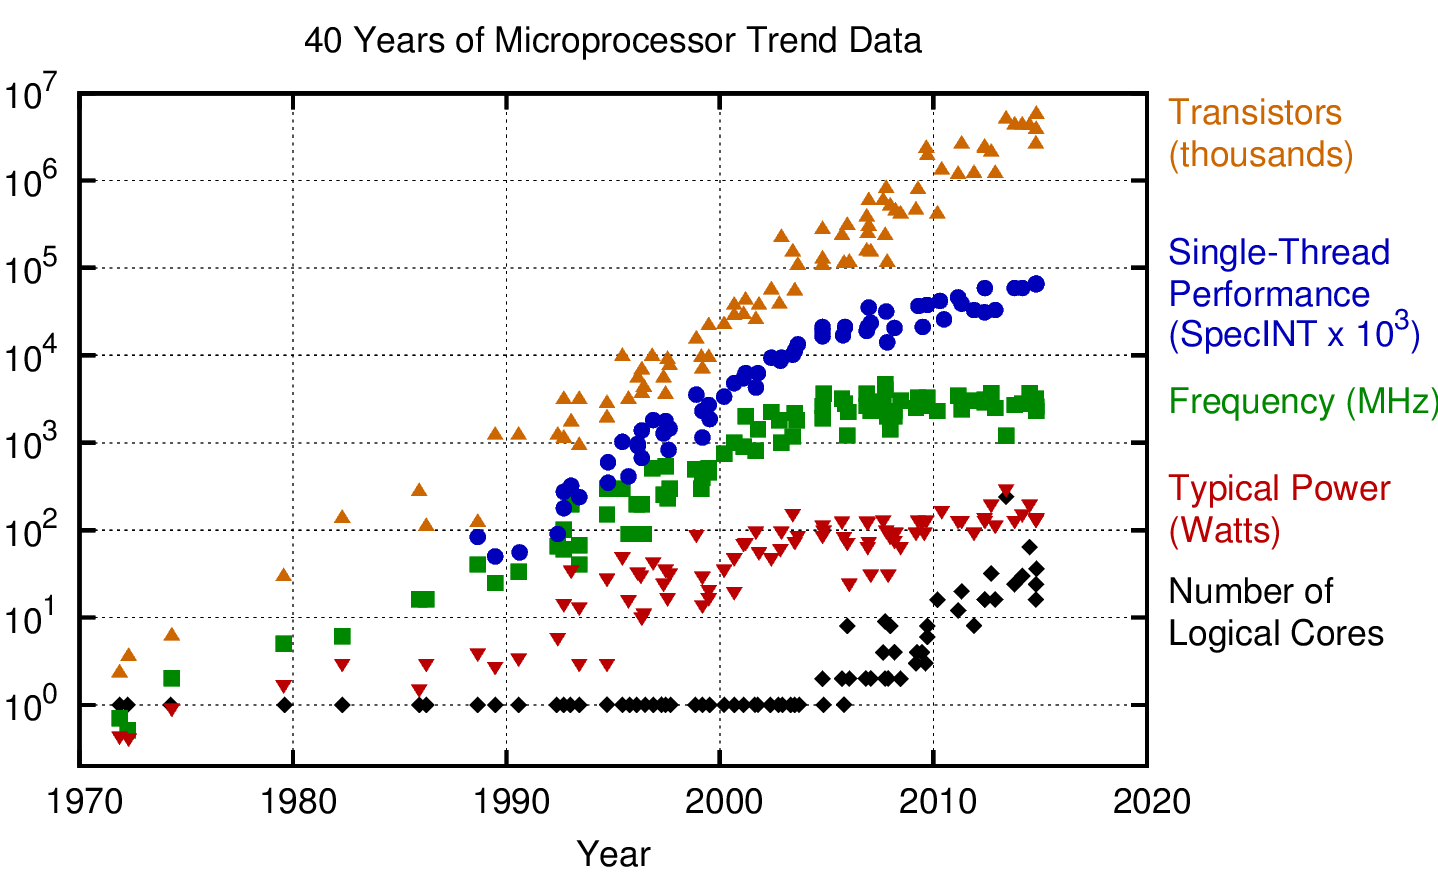
\includegraphics[width=10cm]{images/cpu_evolution.png}
    \caption{\label{pic_cpu_evolution} Évolution des caractéristiques des processeurs \cite{rupp40years}.}
\end{figure}

\begin{figure}
    \center
    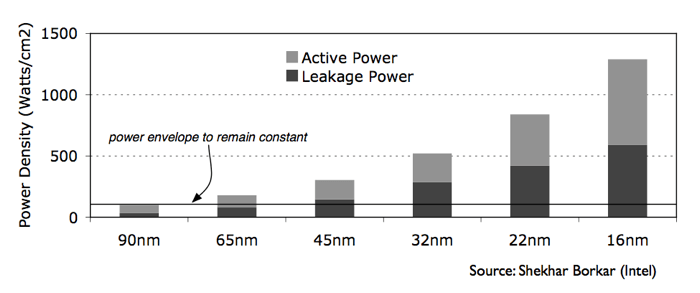
\includegraphics[width=10cm]{images/cpu_leakage.png}
    \caption{\label{pic_cpu_leakage} La miniaturisation de l'isolant nécessaire au fonctionnement des transistors permet le passage de courant de \textit{fuites}.}
\end{figure}

Bien que la fréquence des processeur n'augmentent plus depuis plus de 10 ans, la \autoref{pic_cpu_evolution} montre que la performance des processeurs continue bien d'augmenter. En effet, si la loi de Dennard n'est plus valide, la loi de Moore elle l'est encore après 2005. Les processeurs reçoivent toujours plus de transistors permettant d'augmenter la complexité des pipelines. Ces transistors sont alors utiliser pour construire des processeurs a plusieurs coeurs, présentés dans la \autoref{sec:multicore} (on remarquera que l'augmentation du nombre de coeurs commence exactement quand la fréquence n'augmente plus). Les processeurs sont alors capable de réguler la chaleur d'un processeur en plaçant les processus peu actifs sur les points chauds de la puce.
Pour limiter la consommation électrique, des techniques de management d'alimentation sont alors mises en place pour éteindre certaines parties du processeur inutilisées.
L'utilisation de différentes fréquences est aussi largement utilisée. Les processeurs possèdent des fréquences dites \textit{turbo}, leur permettant d'atteindre des fréquences très élevées pendant un cours laps de temps ou lorsque le processeur n'est pas pleinement utilisé (coeurs et calculs vectoriels inutilisés).



\subsubsection{FPU}\label{sec:fpu}


L'unité de calcul en virgule flottante (FPU pour \textit{floating-point  unit}) est un composant du processeurs permettant de réaliser les opérations sur les nombres à virgule flottante. A l'origine ce module était séparé du processeur et il convenait à l'utilisateur de choisir si il voulait ou non en brancher une sur la carte mère dans l'emplacement qui lui était alors dédié. Pour des questions de coûts d'intégration et de performance, la FPU est depuis 1989, avec la sortie du processeur Intel 80486,  intégrée au processeur. 

Au fil des années la complexité de la FPU a augmenté, quand elle n'était capable d'exécuter que de simples opérations à l'origine, elle peut désormais réaliser des opérations complexes (division, racine carrée, exponentielles ou des fonctions trigonométriques).  De plus, des instructions fusionnées ont fait leur apparition en 2013 dans les processeurs \textit{Haswell} de Intel et Piledriver pour AMD. Elles ont la particularité de réaliser 2 opérations en un seul cycle d'horloge du processeur. Connues sous le nom de FMA pour \textit{fused multiply-add} elles sont capables d'exécuter l'instruction $a \leftarrow b * c + d$ en un seul cycle. 

Enfin, les unités de calcul modernes sont capable d'exécuter une opération sur plusieurs données à la fois ce type d'instructions est dit \textit{vectoriel}. Ces instructions sont performantes pour les algorithmes qui doivent exécuter une même opération sur plusieurs données (un vecteur par exemple). L'évolution de leurs caractéristiques sont abordées dans la partie \ref{sub_taxonomie}.
Les différentes évolution de la FPU sont responsable de la forte augmentation de la puissance de processeur. En effet, usuellement la puissance d'un processeur est donnée par le nombre de calculs flottant qu'il peut exécuter par cycle. Le tableau \ref{tab_FPU} montre comment le nombre de FLOP par cycle évolue: Pour Intel, cette performance a été multipliée par deux à chaque nouvelle version de l'architecture et les FPU modernes exécutent 8 fois plus de calculs qu'en 2008.

\begin{table}[]
\centering
\caption{Evolution de la performance des FPU}
\label{my-label}
\begin{tabular}{|l|l|l|l|l|l|}
\hline
\multicolumn{1}{|c|}{\textbf{Année}} & \multicolumn{2}{c|}{\textbf{Architecture Intel / AMD}}     & \multicolumn{1}{c|}{\textbf{Simpe p.}} & \multicolumn{1}{c|}{\textbf{Double p.}} & \multicolumn{1}{c|}{\textbf{Opérations}} \\ \hline
2008                                 & Nehalem                          & K10                     & 8                                      & 4                                       & 4 add. et 4 mul.         \\ \hline
2011                                 & Sandy Bridge                     & Bulldozer               & 16                                     & 8                                       & 8 add. et 8 mul.         \\ \hline
2013                                 & Haswell \& Skylake               &                         & 32                                     & 16                                      & 8 FMA (mult. + add.)        \\ \hline
2016                                 & Xeon Phi KNL &                         & 64                                     & 32                                      & 8 FMA (mult. + add.)        \\ \hline
\end{tabular}
\label{tab_FPU}
     \vspace{1ex}

     \raggedright Avec Haswell le nombre d'instructions exécutable n'évolue pas mais c'es le type d'instructions exécuté qui sont des FMA (une multiplication et une addition en un cyle d'horloge) et qui correspond à deux FLOP.
\end{table}

\textbf{TODO} latence des differentes instructions; skylake FMA 4 cycles %http://agner.org/optimize/blog/read.php?i=415 (calc_fma() combien de FMA en parallele)







\subsubsection{Optimisations}

Dans les sous-parties précédentes est présenté comment l'évolution de la fréquence et l'utilisation de matériel spécialisé comme une FPU permet d'accélérer l'exécution d'une instruction. Pour différentes raisons (dépendance, manque d'une opérande), les instructions ne peuvent pas être exécutées à la vitesse maximale théorique prévue par le processeur. Pour maximiser le nombre d'instructions exécutées chaque cycle, les processeurs ont reçu de nombreuses optimisations. 

\paragraph{Exécution dans le désordre.}\label{sec:out_of_order}

Le but de cet optimisation est de cacher l'attente de donnée du processeur de la mémoire. Cette avancée est apparue sur les processeurs Intel en 1995 avec le \textit{Pentium P6}. Le principe de l'exécution dans le désordre est d'exécuter les instructions dans un ordre différent que celui donné par le code source.  Ainsi lorsqu'une instruction doit attendre une donnée, au lieu de perdre des cycles à attendre ces données, le processeur va exécuter les instructions qui suivent et finira d'exécuter la première quand la donné sera chargée dans un registre. 
Cependant ne pas exécuter le programme dans l'ordre initial peut fausser les résultats. C'est alors au processeur de s'assurer que les instructions permutées ne sont pas dépendantes. Il existe trois types de dépendances. La première est une \textit{lecture après écriture} (Read After Write ou RAW): une instruction lit une donnée écrite par une instruction la précédent. La deuxième est une \textit{écriture après lecture} (WAR): une première instruction lit une donnée qui est modifiée par une instruction la suivant. Enfin, la dernière dépendance est une \textit{écriture après écriture} (WAW): deux instructions écrivent sur la même donnée. Pour éliminer ces deux dernières dépendances, les processeurs possèdent plus de registres que ceux adressable par le programme. Il les utilise pour éliminer les dépendances WAR et WAW grâce à des techniques de renommage de registres \cite{903248}. 
L'extrait de code \ref{code_dependances} donne un exemple pour chaque type de dépendances. Dans chaque cas, la valeur de B n'est pas la même si les deux assignations ne sont pas exécutées dans le même ordre, suivant cet ordre, B peut valoir 10 ou 15. Pour ce faire, le processeur possède une fenêtre de plusieurs instructions, aussi appelée (à tord) l'\textit{execution queue}. En effet, cette liste n'a pas vocation à être executé dans l'ordre, c'est un rassemblement d'instructions qui ont des dépendances entre elles. Le processeur vient mettre à jour cette liste pour essayer d'exécuter des instructions qui n'ont plus de dépendances avec une donné ou une autre instruction.
Pour pouvoir bénéficier de l'exécution dans le désordre, le processeurs doit donc détecter si les instructions sont dépendantes pour pouvoir les réordonner. Aussi, le programmeur peut aider le processeur dans son travail en évitant au maximum les dépendances entre les instructions. 
La complexité apporté par le système d'exécution dans le désordre, peut être la source d'attaque comme la récente faille \textit{Meltdown} des processeurs Intel \cite{DBLP:journals/corr/abs-1801-01207}.


\begin{lstlisting}[language=C, caption=Exemples de dépendances entre deux instructions., float,floatplacement=H, label=code_dependances]
//----------- Read after Write -----------
int A, B = 0
A = 5;
B = A + 10;
//Result: B == 10 ou B == 15

//----------- Write after Read -----------
int A, B = 0
B = A + 10;
A = 5;
//Result: B == 10 ou B == 15 
 
//----------- Write after Write -----------
int B = 0
B = 10;
B = 15;
//Result: B == 10 ou B == 15
\end{lstlisting}






\paragraph{Prédiction de branchement}\label{sec:branch_predictor}
L'exécution dans le désordre fonctionne tant que suffisamment d'instructions sont disponible pour être exécutées. Cependant, lorsqu'un programme contient un branchement conditionnel, le processeur doit attendre que sa condition soit testée. Si cette condition utilise une variable modifiée dans les instructions précédentes le processeur doit attendre d'avoir le résultat du test pour connaître les futures instructions à exécuter. Pour maximiser l'utilisation du pipeline, le processeur peut essayer de prédire le résultat du test et ainsi continuer l'exécution. S'il s'est trompé sur la prédiction, il doit alors annuler les instructions déjà exécutées et reprendre l'exécution des autres instructions. Le temps nécessaire pour la reprise de l'exécution après une mauvaise prédiction dépend donc de la taille du \textit{pipeline} utilisé (plusieurs dizaines de cycles).
La prédiction de branchement peut être implémentée par deux méthodes.
Le processeur peut posséder un matériel spécifique, appelé prédicteur de branchement (\textit{branch predictor}), qui utilise des méthodes de statistiques. Lorsqu’un branchement est faux plusieurs fois d’affilés, il peut estimer qu'il y a une grande probabilité qu'il le soit aussi à l’itération suivante et éviter d’attendre le résultat du test pour continuer l’exécution. Le processeur peut aussi, à partir de l'adresse de destination, comprendre si la condition et le saut est utilisé dans une boucle ou si c'est un retour de fonction. Une mauvaise prédiction pouvant fortement impacter l'exécution, les processeurs implémentent des prédicteurs de branchement toujours plus complexes. Ce matériel représente une part non négligeable du processeur, et des travaux ont pour objectif d'en comprendre leur fonctionnement \cite{Milenkovic2002}.
La deuxième façon d'implémenter la prédiction est réalisé statiquement, par le compilateur. À la lecture du code, le compilateur peut deviner qu'une boucle ne verra sont branchement vrai qu'a la fin de son parcours. Il peut alors calculer le nombre d’itération à réaliser et éviter le test à chaque itération.
Comme pour le mécanisme d'exécution dans le désordre, la complexité apportée par le prédicteur de branchement a donné lieu à une importante faille de sécurité découverte en 2018 par les chercheurs de Google appelée Spectre \cite{kocher2018spectre}.






%%%%%%%%%%%%%%%%%%%%%%%%%%%%%%%%%%%%%%%%%%%%%%%%%%%%%%%%%%%%%%%%%%%
\subsection{Exécuter les instructions en parallèles} \label{sec:para}
%%%%%%%%%%%%%%%%%%%%%%%%%%%%%%%%%%%%%%%%%%%%%%%%%%%%%%%%%%%%%%%%%%%

La loi de Moore à assurer aux processeurs un gain constant de transistors chaque année. Ils peuvent être utilisés pour implémenter de nouvelles fonctionnalités matériels permettant d'exécuter les instructions en parallèles pour accélérer les applications. Les processeurs ont reçu de nombreuses améliorations dont les principales sont présentées dans cette section: 
\begin{itemize}
    \item Le pipeline
    \item Les processeurs superscalaire
    \item Les coeurs
\end{itemize}


\subsubsection{Le pipeline} \label{sec:pipeline}
%%%%%%%%%%%%%%%%%%%%%%


\paragraph{Motivations.} 

L'utilisation d'instructions CISC toujours plus complexes, a pour effet d'allonger le temps nécessaire à leur exécution qui dure alors plusieurs cycles. Les instructions complexes nécessitent plusieurs opérations: le chargement depuis la mémoire (\textit{fetch}), le décodage (\textit{decode}), le chargement des données nécessaire (\textit{memory}), l'exécution (\textit{execute}) et l'enregistrement du résultat (\textit{write-back}). Pendant ces différentes étapes, la totalité de l'unité d'exécution ne peut pas être utilisée simultanément et l'unité d'exécution n'est pas disponible pour les instructions suivantes. 

La chaîne de traitement du processeur, ou \textit{pipeline}, est une implémentation matériel d'un module qui permet de découper l'exécution d'une instructions en plusieurs étapes (\autoref{pic_pipeline_simple}). Cette technique peut être vu pas analogie à l'utilisation de chaîne de montage. Datant de plus d'un sciècle, la technique de la chaîne de montage a été abondamment utilisée par des industriels tels que Louis Renault et Henry Ford \cite{wolff1957entrepreneurs}.



\begin{figure}
    \center
    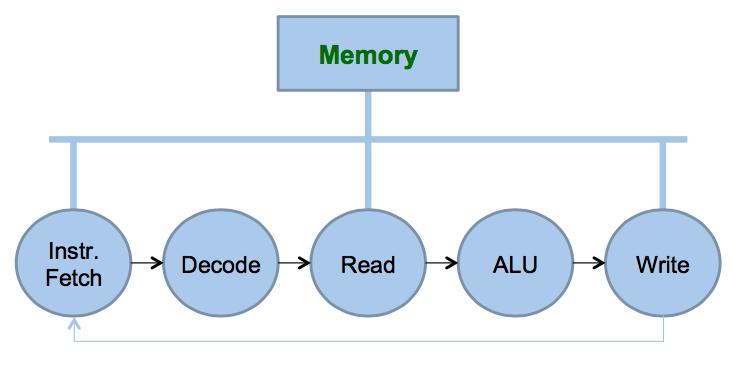
\includegraphics[width=10cm]{images/Chapitre1/Neumann.png}
    \caption{\label{pic_pipeline_simple} Représentation simplifié d'un pipeline de 5 étapes.}
\end{figure}


\paragraph{Implémentation}

En informatique, la technique de \textit{pipeline} est utilisée pour exploiter la parallélisme d'instructions (ILP) (\autoref{pic_pipeline}). Il est commun de présenter la notion de pipeline avec un pipeline de 5 niveaux:

\begin{itemize}
    \item \textbf{Recherche de l'instruction} ou \textit{fetch}: cette première étape charge l'instruction à exécuter depuis la mémoire principale dans un registre du processeur. Grâce à un compteur interne, le registre \textit{Program Counter}, le processeur connaît l'adresse mémoire de la prochaine instruction à charger. Pour améliorer le temps d'accès aux instructions, le processeur possède un tampon (\textit{instruction buffer}) contenant plusieurs instructions d'avance. Ce tampon permet l'implémentation d'optimisations tel que l'exécution dans le désordre (voir \autoref{sec:out_of_order}).
    \item \textbf{Décodage} ou \textit{décode}: une fois que l'instruction est chargée elle est décodée pour déterminer l'action à exécuter et les données nécessaires.
    \item \textbf{Execution} ou \textit{execute}: en fonction du décodage réalisé, l'instruction est exécutée: utiliser l'ALU pour faire une opération ou calculer une adresse.
    \item \textbf{Accès mémoire} ou \textit{memory}: réalise un accès mémoire (\textit{load} ou \textit{store}) lorsqu'une instructions le nécessite.
    \item \textbf{Ecriture du résultat} ou \textit{write back}: Enfin le processeur doit enregistrer le résultat produit par l'étape \textit{execute}. Si c'est un branchement, il modifie le registre \textit{Program Counter} (\textit{branch}). Si c'est une opération arithmétique il sauvegarde le résultat dans l'adresse destinataire décodé par la deuxième étape.
\end{itemize}

Le fait de partager l'exécution d'une instruction en sous étapes permet de commencer l'exécution de la suivante pendant que l'instruction actuelle est encore dans la chaîne d'exécution (voir figure ~\ref{pic_pipeline}). Son utilisation ne réduit pas le temps d'exécution d'une instruction (5 cycles sur la \autoref{pic_pip_no}). Celles-ci doivent tout de même passer une à une par chaque étape de la chaîne. Le \textit{pipeline} permet d'améliorer la cadence d'exécution en maximisant l'utilisation de chaque ressource à un même moment (\autoref{pic_pip_yes}). On peut par exemple commencer à charger la prochaine instruction (étape \textit{fetch}), alors que l'instruction actuelle est en train d'être exécutée (étape \textit{execute}). Sur la \autoref{pic_pip_yes} on assiste à l'exécution de 5 instructions, au premier temps un seul instruction est exécutée, à l'étape $IF$ pour \textit{instruction fetch}. Ensuite (ligne suivante) une nouvelle instruction est chargé (opération $IF$) pendant que la première est passé à l'étape suivante (opération $ID$). Ainsi au bout de 5 cycles, chaque étape du pipeline est utilisée (partie en verte). 


\begin{figure}
    \begin{subfigure}[]{0.5\linewidth}\centering
        \vspace{1.6cm}
        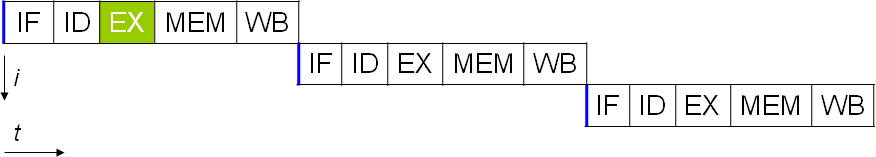
\includegraphics[width=\linewidth]{images/Chapitre1/pipelineNo.png}
        \label{pic_pip_no}
        \caption{Processeur sans pipeline}
    \end{subfigure}%
    ~ %space
    \begin{subfigure}[]{0.5\linewidth}\centering
        \includegraphics[width=.7\linewidth]{images/Chapitre1/pipelineYes.png}
        \caption{Processeur avec un pipeline à 5 étages}
        \label{pic_pip_yes}
    \end{subfigure}
    
    \caption{Pipeline: en séquençant les instructions le processeur est capable d'exécuter des étapes différentes en parallèles (\textit{IF: instruction fetch, ID: instruction decode, EX: execution, MEM: memory, WB: write back}). Le nombre de cycle nécessaire pour l'exécution de 3 instructions passe alors de 15 à 8 cycles (source: \url{https://fr.wikipedia.org/wiki/Pipeline_(architecture_des_processeurs)} }
    \label{pic_pipeline}
\end{figure}




\paragraph{Taille du pipeline.}
En 1939 IBM conçoit le premier processeur avec pipeline. Ce n'est qu'en 1989 qu'Intel produira le siens (Intel 80486). Le nombre d'étapes, ou profondeur du pipeline, était de 2 à l'origine et a augmenté au fil du temps atteignant 31 étapes pour l'architecture du Pentium 4 Prescott d'Intel en 2004. 

\paragraph{Complexité de la gestion du pipeline.}
L'utilisation d'un \textit{pipeline} n'est pas toujours optimale et plusieurs facteurs peuvent affecter sa performance. le principe du pipeline repose sur le concept de commencer à exécuter des instructions avant que la précédente ne soit terminée. Cela peut être rendu impossible par la dépendance entre deux instructions et par l'utilisation de branchements conditionnels \cite{emma1987characterization}. Lors de l'évaluation d'un tel branchement, le pipeline ne peut pas commencer à exécuter les instructions suivantes sans connaître son résultat. Le processeur doit alors attendre (\textit{stall}) plusieurs cycle avant de continuer. Une optimisation de prédiction de branchement a été implémentée pour éviter ces états de \textit{stall} (voir \autoref{sec:branch_predictor}). De plus, pour permettre la bonne utilisation du pipeline, des mémoires tampons doivent être disposées entre chaque étapes pour mémoriser les différents résultats intermédiaires. Lorsque le processeur exécute plusieurs processus, il doit veiller à terminer l'exécution des instructions avant de commencer celles du processus suivant. La complexité de sa gestion le rend vulnérable aux attaques informatiques (voir \autoref{sec:out_of_order}). 












\subsubsection{Processeur superscalaire} \label{sec:superscalar}
%%%%%%%%%%%%%%%%%%%%%%

Le pipeline apporte un niveau de parallélisation horizontale. Les processeurs ont reçus une autre amélioration apportant au pipeline une parallélisation verticale. 

\paragraph{Principe}
Un processeur est dit \textit{superscalaire} s'il est capable d'exécuter plus d'une instruction simultanément. Le nombre d'instruction par cycle d'holorge (IPC) peut alors être supérieur à 1. Le principe est d'implémenter un second pipeline (ou plus) capable d'exécuter les instructions tel que sur la \autoref{pic_pip_yes}. Intel proposa son premier processeur superscalaire en 1989 avec le processeur Intel 80486. Il possédait un pipeline à cinq étages proche de celui présenté dans la section précédente. 
Pour pouvoir l'utiliser, le processeur doit déterminer si deux instructions peuvent être exécutées en parallèle (sans dépendance et utilisant des ressources matériels différentes). La \autoref{pic_superscalar} montre comment une implémentation superscalaire du pipeline fonctionne. 

\begin{figure}
    \center
    \includegraphics[width=8cm]{images/Chapitre1/superscalar.png}
    \caption[Processeur superscalaire]{Fonctionnement d'un processeur superscalaire possédant deux pipelines.\protect\footnotemark. \label{pic_superscalar} }
\end{figure}
\footnotetext{source: \url{https://fr.wikipedia.org/wiki/Processeur_superscalaire}}

\paragraph{Implémentation}
Il existe deux façons de transformer un processeur scalaire en superscalaire. La première est de dupliquer matériellement chaque étape pour obtenir deux pipelines distincts (processeurs \textit{superpipeline}). On peut citer le processeur Intel Pentium dont la totalité du pipeline n'est pas dupliqué. Le processeurs à une fenêtre de plusieurs instructions prêtes à être exécutées. Seule la phase d'exécution est dupliquée.  Il possédait deux unités d'exécution \textit{u} et \textit{v} qui pouvait exécuter des instructions de types différents (opérations flottantes ou entières) en parallèle. 
Le deuxième moyen d'implémenter le parallélisme d'instruction d'un processeur superscalaire repose sur le fait qu'une étape peut nécessiter moins d'un demi cycle d'horloge pour être exécutée. Une étape (ou micro-instruction) du pipeline peut donc s'occuper de deux instructions différentes pendant un cycle d'horloge, en utilisant sa propre horloge interne. Cette méthode à le bénéfice de ne pas avoir a dupliquer le pipeline matériellement. 

Les principales limitations à l'implémentation d'un pipeline sont les dépendances et les conflits. Cela peut être une dépendance entre les données de plusieurs instructions ou un conflits d'accès à une même ressource (ALU, FPU). Le processeur est alors en charge d'orchestrer les différentes instructions pour rendre possible le parallélisme en utilisant des \textit{stratégie d'iméssion} \cite{johnson1989super} des instructions. Cette stratégie doit veiller à conserver la validité du programme en veillant aux ordres: de lecture des instructions, de leur exécution et de leur actualisation des registres (ou de la mémoire). 


\paragraph{Exemple du Pentium 4}
Pour bien comprendre le déroulement de l'exécution du pipeline d'un processeur superscalaire, nous choisissons de détailler le fonctionnement de processeur Intel Pentium 4 \cite{stallings2003organisation} donc le schéma de la micro-architecture est présenté sur la \autoref{cpu_superscalar_pentium}. Le processeur exécute les \textit{micro-ops} en utilisant un pipeline d'au moins 20 étages en veillant à respecter les dépendances, dont les principales étapes sont décrites ici: 

\begin{enumerate}
    \item Le processeur lit les instructions (CISC) depuis le cache L2 par groupe de 64 octets dans l'ordre du programme pour profiter de l'effet de localité. Bien que la prédiction de branchement puisse modifier cet ordre. 
    \item Chaque instruction (pouvant être de taille différente) est décodé et traduite en une à quatre instructions RISC de 118 bits (\textit{micro-ops}). \item Ces micro-ops sont ensuite stockées dans un buffer (\textit{Trace Cache}) permettant l'utilisation de l'exécution dans le désordre (voir \autoref{sec:out_of_order}).
    \item Ensuite, le processeur possède au renommage des registres. Il existe 16 registres architecturaux (utilisable pas le code) mais 128 registres physique sont réellement implémentés. Les \textit{micro-ops} peuvent ensuite être stockée dans deux listes d'attente distinctes utilisant une discipline \textit{FIFO}.
    \item L'ordonnanceur choisi ensuite dans les deux files les instructions qui possèdent leurs opérandes et dont l'exécution peut être réalisée. Suivant le type d'instruction elle sont envoyées (jusqu'à 6 à la fois) vers l'unité d'exécution correspondante (calcul entier ou flottant) en utilisant les différents ports. 
\end{enumerate}
     

\begin{figure}
    \center
    \includegraphics[width=13cm]{images/cpu_superscalar_pentium.png}
    \caption[Diagramme en bloc du Pentium 4]{Diagramme en bloc du Pentium 4 \cite{stallings2003organisation}
    \label{cpu_superscalar_pentium}}
\end{figure}



Les architectures actuelles otn beaucoup évoluées depuis le premier pentium. Le détail de la micro-architecture Skylake d'Intel peut être consultée sur la \autoref{pic:cpu_skylake_architecture}. L'unité d'exécution peut être utilisée par 8 \textit{ports} différents. Chaque port est relié à des composants différents de l'ALU qui peut exécuter jusqu'à 4 instructions par cycles (ou 2 opérations flottantes).






\subsubsection{Processeur multi-coeurs} \label{sec:multicore}
%%%%%%%%%%%%%%%%%%%%%%


\paragraph{Motivation.}
La vitesse de calcul d'un processeur est lié à sa fréquence qui a largement contribué à l'évolution de leur performance. Cependant, certaines limites physiques empêchent l'augmentation infinie des fréquences (discuté dans la partie \ref{sec:frequence}). Il a donc fallu trouver d'autres moyens d'améliorer la performance des processeurs, sans pouvoir accélérer leur fréquence. L'apparition des processeurs multi-coeurs est une réponse à ce challenge. Pour comprendre leur intérêt l'analogie suivante peut être utilisée \cite{tanenbaum2016structured}: la construction d'un processeur avec une fréquence de 1000 GHz est probablement impossible. Par contre l'utilisation de 1000 processeurs avec une fréquence de 1 Ghz est possible pour obtenir la même performance. Ce gain de performance peut alors être utilisé pour réduire la fréquence des processeurs. En réduisant la fréquence de 30\%, l'énergie nécessaire est elle réduite de 35\% \cite{mattsson2014haven}. En utilisant deux coeurs à 70\% de la fréquence initiale permet cependant d'obtenir un gain de 140\% de la puissance de calcul. C'est ce constat qui motive l'utilisation du parallélisme dans toute l'architecture d'un supercalculateur (voir \autoref{sec:parallelisme}). Ainsi, avant l'apparition des processeurs mutli-coeurs, l'utilisation du multitraitement symétrique (SMP) utilisant plusieurs processeurs en parallèles était le principale moyen d'accéder au parallélisme. Cependant, les serveurs devenant toujours plus gros, et avec le désir d'avoir des processeurs plus puissant pour les ordinateurs personnelles et les téléphones, les processeurs multi-coeurs ont été inventés.


\paragraph{Multi-coeur.}
Le terme de processeur multi-coeur est employé pour désigner tout processeur possédant entre deux et quelques dizaines de coeurs (on parle de processeurs \textit{manycore} au delà). Les différents coeurs sont disposés sur la même puce d'où l'autre appellation utilisée pour désigner ces processeurs de Chip Multiprocessor (CMP).
Les différents coeurs sont généralement identiques en tout point (processeur homogène) bien qu'ils puissent être différents (processeur hétérogène). Les processeurs homogènes sont plus faciles à utiliser car tous les coeurs peuvent répondre au même besoin et leur design est plus simple. Les processeurs hétérogènes sont cependant plus performant pour certaines application. 
Généralement, chaque coeur du processeur n'est pas relié directement à la mémoire. Un niveau de cache est généralement interposé entre le coeur et la mémoire. La hiérarchie mémoire est présentée dans la \autoref{sec:hierarchie}.

\begin{figure}
    \center
    \includegraphics[width=10cm]{images/cpu_multicore.jpg}
    \caption{\label{processeur_archi} Exemple de processeur multi-coeur (Intel Core i7-2600K)  partageant le troisième niveau de cache.\protect\footnotemark}
\end{figure}

\footnotetext{source: \url{https://www.anandtech.com/show/4083/the-sandy-bridge-review-intel-core-i7-2600k-i5-2500k-core-i3-2100-tested}}




L’avantage principale de dupliquer un coeur plutôt que de doubler la fréquence d’un seul coeur est la consommation électrique et donc la puissance dégagée par effet Joule. En effet, la puissance dissipée est quadruplée quand la fréquence est doublé alors qu'elle ne fait que doubler lorsque que le nombre de coeur est doublé. On obtient ainsi un processeur utilisant moins d’énergie et nécessitant moins de refroidissement pour une même performance qu'un processeur plus rapide.
Comme pour le pipeline (voir \autoref{sec:pipeline}), le gain de performance apporté par l’ajout de coeur s’appuie sur l’amélioration du parallélisme d'instruction (Instruction Level Parallélisme (ILP)).

La difficulté d’utilisation de processeurs multi-coeurs vient des programmes qui ne sont pas capables par nature d’utiliser ce niveau de parallélisme. Ils doivent donc être programmés pour pouvoir en profiter. Cette tâche, quoique difficile à ses début, est aujourd'hui facilitée par l’utilisation de librairies prévues telles que \textit{Pthread} ou \textit{OpenMP}. 

Les coeurs partageant des niveaux communs de cache (généralement le dernier), la bonne programmation des applications et l'implémentation d'une micro-architecture efficace sont alors des facteurs déterminant de la performance obtenue:
\begin{itemize}
    \item Pour maximiser l'utilisation des caches, il est primordiale de prévoir leur partages entre les différents coeurs pour minimiser les conflits. Des méthodes de placements plus ou moins efficaces peuvent alors être utilisées \cite{mazouz2011performance}: laisser le système d'exploitation peut donner des performances très variable entre deux exécutions identiques, alors que le placement manuel permet d'obtenir les meilleurs résultats. 
    \item Le choix du réseaux utilisé par les coeurs est alors important pour la performance des codes et repose principalement sur quatre paramètres \cite{peh2009chip} : la topologie, les algorithmes de routages, le protocole de contrôle de flux et le routage de la micro-architecture. La topologie indique comment les coeurs sont connectés et quels sont les chemins empruntable pas un message pour rejoindre sa destination. Ce choix est réalisé par l’algorithme de routage. Le contrôle de flux s’occupe de l'envoi des messages (ordre et date d’envoie) qui est ensuite réalisé par la micro-architecture. Les choix réalisés pour ces quatre paramètres ont un impact sur la performance du processeur (latence, bande passante) et sur son prix. 

\end{itemize}


Le nombre de coeurs par processeur a beaucoup évolué dans les quinze dernières années. Si les premiers processeurs multi-coeurs n'en possédaient que deux, il n'est pas rare que les supercalculateur utilisent des processeurs avec plus de vingt coeurs. Intel à même annoncé en 2019 un nouveau processeur doté de 56 coeurs \footnote{\url{https://ark.intel.com/content/www/us/en/ark/products/194146/intel-xeon-platinum-9282-processor-77m-cache-2-60-ghz.html}}. Cependant, l'ajout de coeurs supplémentaires n'est pas forcément bénéfique pour les applications à cause de la vitesse des mémoires qui peinent à évoluer au même rythme. Ce constat est discuté dans la \autoref{sec:memorygap}.





























%%%%%%%%%%%%%%%%%%%%%%%%%%%%%%%%%%%%%%%%%%%%%%%%%%%%%%%%%%%%%%%%%%%
\section{Hiérarchie mémoire} \label{sec:hierarchie}
%%%%%%%%%%%%%%%%%%%%%%%%%%%%%%%%%%%%%%%%%%%%%%%%%%%%%%%%%%%%%%%%%%%

\begin{fancyquotes}
Idéalement, on souhaiterait disposer d'une capacité de mémoire indéfiniment grande, de sorte qu'un agrégat particulier de 40 chiffres binaires, ou mot (cf. 2.3), soit immédiatement disponible, c'est-à-dire dans un temps légèrement ou considérablement plus court que le temps de fonctionnement d'un multiplicateur électronique rapide. On peut supposer que cela est pratique au niveau d'environ 100 m sec. Par conséquent, le temps de disponibilité d'un mot dans la mémoire doit être de 5 à 50 ms. Il est également souhaitable que les mots puissent être remplacés par de nouveaux mots à peu près au même rythme. Il ne semble pas physiquement possible d'atteindre une telle capacité. Nous sommes donc obligés de reconnaître la possibilité de construire une hiérarchie de mémoires, chacune d'entre elles ayant une plus grande capacité que la précédente mais moins rapidement accessible.\\
Traduit de \cite{burks1946preliminary}.

\end{fancyquotes}


\subsection{Motivations}
%%%%%%%%%%%%%%%%%%%%%%%%%%%%%%%%%%%%%%%%%%%%%%%%%%%%%%%%%%%%%%%%%%%


Dès 1946, les architectes des processeurs avaient anticipé que les applications seraient demandeuses de mémoires très performantes. A cause de la forte évolution du processeur, l'écart avec la performance des mémoires s'est creusé au fil des années (voir \autoref{pic:cpuvsmemory}). L'incapacité du processeur d'accéder suffisamment rapidement à la mémoire est inhérent à l'architecture actuelle des processeurs qui partage le même bus pour accéder aux instructions et aux données stockées en mémoire. Ce \textit{goulot d'étranglement} ou \textit{bottleneck}, a été nommé d'après l'un des architectes de l'architecture: le \textit{bottleneck Von Neumann}.


\begin{figure}
    \center
    \includegraphics[width=10cm]{images/cpu_vs_memory.png}
    \caption{\label{pic:cpuvsmemory} Progression de la performance des processeurs et des mémoires. Les processeurs ont vu leur performance évoluer de 50\% chaque année, contre 7\% pour les mémoires. L'écart de performance entre les deux matériels s'est creusé de 50\%  chaque année depuis les années 2000 (graphique extrait de \cite{AliSalehi2012}).}
\end{figure}

La réponse naïve à ce problème est de construire de grande mémoire à partir de SRAM, très performante et qui consomme peu d'énergie. Cependant, des contraintes économiques et technique sont à prendre en compte et rendent impossible cette solution. La mémoire SRAM est très cher à produire et nécessite l'utilisation de six transistors pour fonctionner, empêchant la construction de modules denses. Les constructeurs de processeurs ont dû élaborer une solution en prenant en compte la vitesse, la densité et le coût de chacune des technologies mémoires. Au plus une mémoire est rapide, au plus sont coût est élevé. Au plus la densité est élevée, plus le prix par bit stocké est réduit. Au plus la densité est élevé, au plus le temps d'accès est élevé. 






\subsection{Hiérarchie mémoire sur les processeurs récents}
%%%%%%%%%%%%%%%%%%%%%%%%%%%%%%%%%%%%%%%%%%%%%%%%%%%%%%%%%%%%%%%%%%%

La hiérarchie mémoire est la réponse économique et technique apportée aux contraintes évoquées ci dessus. Elle consiste en l'utilisation de différents modules mémoires de tailles, de technologies et de performances différentes. Son objectif peut être résumé à trois points: réduire le coût par bit stocké, augmenter la capacité de la mémoire la plus rapide, améliorer le temps d'accès aux données. La solution est de placer au plus proche du processeur des mémoires très rapide pouvant répondre instantanément aux accès mémoire. Au plus on s'éloigne des unités de calcul, au plus la latence d'accès aux modules mémoires augmente, mais au plus leur prix diminue rendant possible l'utilisation de module de plus grande capacité.


Les différents niveaux de mémoire peuvent être imbriqués, une donnée qui se trouve dans le premier niveau sera aussi stockée dans les modules de niveaux supérieurs.

Lorsque le processeur souhaite accéder à une donnée, il vérifie qu'elle se trouve dans son premier niveau de mémoire et, si ce n'est pas le cas, remonte la hiérarchie jusqu'à la trouver. La performance des applications varie fortement si les données nécessaires sont présentes ou non dans les mémoires proches du processeur. Les programmes doivent essayer de profiter du concept de localité présenté dans la section \autoref{sec:localite}.
\begin{figure}
    \center
    \includegraphics[width=14cm]{images/memory_hierarchy.png}
    \caption{\label{pic:cpuvsmemory} Hiérarchie mémoire}
\end{figure}





\subsection{Communication entre les différents niveaux}
%%%%%%%%%%%%%%%%%%%%%%%%%%%%%%%%%%%%%%%%%%%%%%%%%%%%%%%%%%%%%%%%%%%
Pour communiquer entre les différents niveaux de la hierarchie les données sont transmises par bloc de données de tailles différentes. L'avantage de tranférer les données par bloc et non une par une est d'amlélirer la performance des codes en tirant parti du principe de localité spatiale (voir \autoref{sec:localite}).
Pour accéder à un mot, le processeur a besoin que celle ci se trouve dans le niveau de cache L1. Lorsqu'elle si trouve, le processeur peut charger un mot directement dans ces registres pour y effectuer les opérations nécessaires. C'est la granularité de transfert la plus petite dans un ordinateur. 

Entre les différents niveaux de caches et entre le cache et la mémoire les données sont transférées par blocs appellées \textit{lignes de cache} ou \textit{cache line}. La ligne de cache contient une copie des données de la mémoire, un tag contenant des informations sur l'adresse mémoire du bloc de donnée et un \textit{flag} contenant des informations sur la validité de la ligne (voir \autoref{pic:cacheline}). La taille d'une ligne de cache peut varier d'une architecture à l'autre mais il est courant d'utiliser des tailles de 32, 64 ou 128 bytes. Une ligne de cache d'un processeur Intel récent mesure 64 bytes. Elle contient ainsi entre 8 et 16 éléments en double précision. 

\begin{figure}
    \center
    \includegraphics[width=8cm]{images/cacheline_def.png}
    \caption{\label{pic:cacheline} Représentation d'une ligne de cache.}
\end{figure}


Entre la mémoire, les blocs de données transférés sont de la taille d'une page (voir \autoref{sec:page}) qui mesure généralement entre 4 KiB et 2 MiB.



\subsection{Registres}
%%%%%%%%%%%%%%%%%%%%%%%%%%%%%%%%%%%%%%%%%%%%%%%%%%%%%%%%%%%%%%%%%%%
Les registres du processeurs sont situés au plus proche des unités de calculs. Pour permettre un accès rapide, 1 cycle, ils sont réalisés en SRAM. On compte entre x et y registres sur les processeurs récents. Leur taille est variable en fonction des instructions exécutables par les unités logiques arithmétiques. Par exemple, un processeur pouvant exécuter des instructions vectorielles AVX-512, possède des registres de 512 bits (registre \textit{ZMM}). Il existe différents types de registres, certains sont utilisés pour stocker des données et des résultats intermédiaires, tandis que d’autres ont une signification précise. Le registre de pointeurs de piles stocke l’adresse de la première adresse mémoire responsable de l’instruction actuellement exécutée et permettent de réaliser des appels et des retours de fonctions. Les registres des drapeaux (Flag Register) stockent des informations nécessaire à l’éxécution d’instructions. Par exmple, lorsqu’une retenue est générée par un calcul, ou qu’un branchement conditionnelle a été évalué à vrai. Les processeurs récents dupliquent certains registres pour pouvoir utiliser des techniques de renommage \cite{moudgill1993register} et d'exécution spéculative \cite{chou2004efficient}. Lors de l'exécution d'une instruction nécessitant plusieurs cycles, le processeur, si aucune dépendance n'est détectée, commence à exécuter les instructions suivantes sans attendre le résultat de la première instruction.






%%%%%%%%%%%%%%%%%%%%%%%%%%%%%%%%%%%%%%%%%%%%%%%%%%%%%%%%%%%%%%%%%%%
%%%%%%%%%%%%%%%%%%%%%%%%%%%%%%%%%%%%%%%%%%%%%%%%%%%%%%%%%%%%%%%%%%%
\subsection{Caches} \label{sec:cache}
%%%%%%%%%%%%%%%%%%%%%%%%%%%%%%%%%%%%%%%%%%%%%%%%%%%%%%%%%%%%%%%%%%%
%%%%%%%%%%%%%%%%%%%%%%%%%%%%%%%%%%%%%%%%%%%%%%%%%%%%%%%%%%%%%%%%%%%
%intro
C’est en 1965 que les premières mémoires caches sont présentées sous le nom de \textit{slave memory} \cite{wilkes1965slave}. Leur temps d’accès est de 4 à 20 fois plus rapide que celui de la mémoire principale servant alors de mémoire tampon. Cependant leur taille est très réduite (quelques MiB) comparée à celle de la mémoire principale (plusieurs GiB). Les cache utilisent généralement de la mémoire SRAM.

%performance
Ce niveau de mémoire a été implémenté pour réduire, du point de vu du processeur, l’écart de performance entre ses unités de calculs et celles de la mémoire centrale. Leur apport de performance vient de la capacité des programmes à réutiliser des données déjà présentes, évitant une accès à la mémoire centrale beaucoup plus long. Lorsque le processeur doit accéder à une donnée, il commence par la chercher dans le premier niveau de cache, si elle si trouve, son temps d'accés est très rapide (évenement \textit{cache hit}). Si ce n’est pas le cas (évenement \textit{chache miss}), il réalise alors une copie de la zone mémoire la contenant dans le cache. La zone mémoire copié est appelé \textit{ligne de cache}. Si par la suite, cette donnée ou une donnée appartement à la même ligne de cache devait être à nouveau accédée, leur temps d’accès serait alors drastiquement réduit. Ce mécanisme est transparent pour l’utilisateur, bien que pour des questions de performances il doive être conscient de son existence (voir \autoref{sec:localite}). 

%taille vs performance
La taille de chaque niveau de cache varie pour les raisons expliquées en introduction de cette partie. A cela vient s'ajouter la notion de performance qui est liée à leur taille. Un cache de grande capacité aura plus de chance de contenir la donnée dont le processeur à besoin, améliorant ainsi la performance moyenne du programme. Un cache est une mémoire associative. Pour accéder à son contenu il faut utiliser une clef associative. La clef est constitué de l’adresse en mémoire centrale de l’instruction ou de la donnée. Un cache plus grand nécessite plus de comparaisons pour vérifier si une donnée s'y trouve ou non. Pour allier les avantages et contourner les inconvénient, les processeurs utilisent non pas un, mais plusieurs niveaux de caches de tailles différentes.
Le premier niveau de cache est généralement séparé en deux zones mémoire: l'une contenant les instructions et l'autre les données. C'est le seul niveau de la hiérarchie qui stocke différemment les données et les instructions. Sur les processeurs récents, le premier et le deuxième niveau de cache est privé à chaque coeur. Un troisième, et parfois un quatrième niveau de cache est partagé entre les différents coeurs du processeur. La \autoref{pic:cache_hierarchy} représente une telle architecture pour un processeur à 4 coeurs. Le partage d’un ou plusieurs niveaux de caches entre différents coeurs à certains bénéfices en programmation parallèle. La communication entre les coeurs est plus rapide, ainsi que la migration d’un thread entre deux coeurs partageant un même niveau de cache. Cependant, cela introduit de la complexité pour la cohérence des caches (voir \autoref{sec:cache_coherence}).

\begin{figure}
    \center
    \includegraphics[width=8cm]{images/cache_hierarchy.png}
    \caption{\label{pic:cache_hierarchy} Organisation d'une hiérarchie de cache à trois niveau sur un processeur à 4 coeurs (source \cite{putigny2014benchmark}).}
\end{figure}




\subsubsection{Propriété d'inclusion}
%%%%%%%%%%%%%%%%%%%%%%%%%%%%%%%%%%%%%%%%%%%%%%%%%%%%%%%%%%%%%%%%%%%
Lorsqu'une donnée est chargé depuis la mémoire, le processeur doit la stocker dans le cache qui varie en fonction de la propriété d'inclusion du processeur pouvant être inclusive ou exclusive ou non-inclusive (voir \autoref{pic:cacheinclusionpolicy}).

Un cache est dit inclusif, si lorsqu'une donnée se trouve à un niveau de la hiérarchie, tous les caches des niveaux supérieur contiennent eux aussi une copie de la donnée (voir \autoref{pic:InclusivePolicy}). Cette politique d'inclusion a un désavantage lorsqu'elle est utilisée sur des système multi-coeurs. En effet, lorsqu'une donnée doit être retiré d'un niveau de cache, le processeur doit aussi l'enlever des niveaux de caches inférieurs. 
Un cache non-inclusif permet qu'une ligne du cache de niveau 1 ne soit pas forcément dans le cache de niveau 2. Cela permet d'augmenter la capacité de la hiérarchie de cache. Les processeurs récents implémente les deux politiques d'inclusion. Le processeur Intel Sandy Bridge a un cache L3 inclusif tandis que les cache L1 et L2 sont non-inclusif.

Pour une politique d'exclusion, une donnée qui se trouve à un niveau du cache, ne peut pas se trouver dans un autre niveau de cache au même moment (voir \autoref{fig:ExclusivePolicy}). L'avantage des caches exclusif est leur capacité de stocker plus de données car une ligne de cache ne se trouve jamais à deux endroits à la fois de la hiérarchie de cache. Cependant, lors d'un \textit{hit} dans le cache L2, le processeur doit échanger la ligne entre les deux niveau de cache L1 et L2, plus long qu'une simple copie.



\begin{figure}
    \centering
    \begin{subfigure}[b]{0.45\linewidth}
        \includegraphics[width=\linewidth]{images/InclusivePolicy.png}
        \caption{Inclusive}
        \label{pic:InclusivePolicy}
    \end{subfigure}
    ~ %add desired spacing between images, e. g. ~, \quad, \qquad, \hfill etc. 
      %(or a blank line to force the subfigure onto a new line)
    \begin{subfigure}[b]{0.45\linewidth}
        \includegraphics[width=0.85\linewidth]{images/ExclusivePolicy.png}
        \caption{Exclusive}
        \label{pic:ExclusivePolicy}
    \end{subfigure}
    \caption{Exemple de deux propriétés d'inclusion de la hiérarchie de cache (source \cite{wikipedia_2019}). }\label{fig:cacheinclusionpolicy}
\end{figure}




\subsubsection{Politique de placement: associativité}
%%%%%%%%%%%%%%%%%%%%%%%%%%%%%%%%%%%%%%%%%%%%%%%%%%%%%%%%%%%%%%%%%%%
La performance d'un cache ne vient pas seulement de la technologie utilisée pour sa construction. En effet, lorsqu'une donnée est accédée, le cache doit vérifier si la donnée est présente ou non dans le niveau de cache demandé. Il faut que l'algorithme de comparaison permettant de la trouver soit le plus rapide possible. Pour cela, les architectes utilisent généralement une fonction de \textit{hash} permettant d'attribuer un emplacement dans le cache en fonction de l'adresse mémoire de la \textit{cache line}. Si la \textit{cache line} ne se trouve pas à l'emplacement calculé, c'est quelle n'est pas présente dans ce niveau de cache.


\begin{figure}
    \centering
    \begin{subfigure}[b]{0.45\linewidth}
        \includegraphics[width=\linewidth]{images/cache_calcul.png}
        \caption{Calcul de l'emplacement (index de la ligne et décalage) pour un mappage direct}
        \label{pic:cache_calcul}
    \end{subfigure}
    ~ %add desired spacing between images, e. g. ~, \quad, \qquad, \hfill etc. 
      %(or a blank line to force the subfigure onto a new line)
    \begin{subfigure}[b]{0.45\linewidth}
        \includegraphics[width=\linewidth]{images/cache_direct.png}
        \caption{Emplacement de la ligne calculée dans le cache ou sera stockée la \textit{cache line}.}
        \label{pic:cache_direct}
    \end{subfigure}
    \caption{Exemple du calcul de l'emplacement de la ligne de cache lors d'un mappage direct à partir de l'adresse de la \textit{cache line} à stocker (source \cite{Meunier2017}). }\label{fig:cacheinclusionpolicy}
\end{figure}





Les trois politiques de placement les plus utilisées sont: le mappage  \textit{direct }, le mappage \textit{fully associative} et le mappage \textit{set assiociative} (voir \autoref{pic:cache_associativite}).


\begin{figure}
    \center
    \includegraphics[width=12cm]{images/cache_associativite.png}
    \caption{\label{pic:cache_associativite} En fonction de la politique de remplacement utilisée, une \textit{cache line} sera associée à une ligne du cache différente (source \cite{Meunier2017})}
\end{figure}

\paragraph{Cache à correspondance directe (\textit{direct-mapped cache})} utilise une fonction simple pour déterminer l'emplacement (index et offset) du cache à utiliser. Une partie des bits le l'adresse de la \textit{cache line} est utilisée pour déterminer la ligne à utiliser (\textit{index}) par exemple à l'aide d'une opération modulo. L'autre partie est utilisée pour déterminer le décalage dans cette ligne (\textit{offset}). Cette méthode est très rapide mais peut avoir des performances catastrophiques. Un algorithme faisant des sauts en mémoire d'une certaine taille pourrait n'utiliser qu'une seule ligne du cache, le rendant totalement inefficace. Comparé aux caches associatifs, le mappage direct est plus simple à implémenter car un seul comparateur est nécessaire pour déterminer la ligne de cache à utiliser (voir \autoref{fig:cache_schema}).

\paragraph{Cache pleinement associatif (\textit{fully associative cache})} remédie à ce problème en permettant à une \textit{cache line} d'être stockée à n'importe quel emplacement dans le cache. Cependant, cette technique à le désavantage d'être très lente. En effet, une \textit{cache line} pouvant se trouver à n'importe quelle ligne du cache, il faut toutes les comparer pour vérifier sa présence ou non. Pour faire cette comparaison en parallèle, il faudrait implémenter autant de comparateurs que de ligne dans le cache, complexifiant grandement le cache.


\paragraph{Cache N-associatif (\textit{N-way set associative cache})} permet de réduire le nombre de comparateurs nécessaires en regroupant les lignes du caches potentiellement adressable pour une \textit{cache line} en groupe (\textit{set}). L'exemple de la \autoref{pic:cache_associativite} utilise un cache à 4 set, appelé \textit{4-way associative}. Il ne faut plus que 4 comparateurs pour déterminer si une ligne appartient à un des \textit{set}. Les mappage par association sont plus lents que le mappage direct, car il faut trouver où se trouve la \textit{cache line} (si présente) dans un sous ensemble de ligne de cache plus ou moins grand. Pour accélérer la recherche de la présence ou non d'une ligne de cache, le traitement peut être réalisé en parallèle dans les différents \textit{sets} par l'utilisation de plusieurs comparateurs (4 dans la \autoref{pic:cache_circuit-set-associative}). 

La propriété principale d'un cache est sa capacité à conserver les données pour de futurs accès. Un cache de 8 MB à 2 set associatifs peu sauver jusqu'à 44\% des \textit{miss} comparé à un cache à correspondance directe \cite{Drepper2007}. Sur les architectures récentes Intel Skylake, les caches utilisent entre 8 et 16 associativités, pouvant varier entre les différents niveaux. 

\begin{figure}
    \begin{subfigure}[t]{\linewidth}\centering
        \includegraphics[width=0.7\linewidth, trim = 0cm 10cm 0cm 2cm]{images/cache_circuit-direct.png}
        \caption{Le cache pleinement associatif nécessite d'avoir un comparateur pour chacune des lignes du cache}
        \label{pic:cache_circuit-direct}
        \vspace{1cm}
    \end{subfigure}
    
    \begin{subfigure}[t]{\linewidth}\centering
        \includegraphics[width=0.7\linewidth]{images/cache_circuit-fully-associative.png}
        \caption{Le cache pleinement associatif nécessite d'avoir un comparateur pour chacune des lignes du cache}
        \label{pic:cache_circuit-fully-associative}
        \vspace{.5cm}
    \end{subfigure}
    
    \begin{subfigure}[t]{\linewidth}\centering
        \includegraphics[width=0.7\linewidth]{images/cache_circuit-set-associative.png}
        \caption{Le cache N-associatif associe les deux architectures des caches direct et pleinement associatif. Ce sont plusieurs caches directs montés en parallèles.}
        \label{pic:cache_circuit-set-associative}
    \end{subfigure}
    
    \caption{Schéma des trois modèles de cache utilisés (tirés de l'ouvrage \cite{Blanchet2013}).}\label{fig:cache_schema}
\end{figure}




\subsubsection{Politique de remplacement}
%%%%%%%%%%%%%%%%%%%%%%%%%%%%%%%%%%%%%%%%%%%%%%%%%%%%%%%%%%%%%%%%%%%
Que ce soit pour le mappage \textit{fully associative} ou \textit{set associative}, une \textit{cache line} peut être stockée dans plusieurs ligne du cache. Pour déterminer laquelle choisir pour y placer la \textit{cache line}, différentes stratégies peuvent être utilisées, appelées \textit{politique de remplacement}. L'objectif de ces politiques est de maximiser l'utilisation du cache en prévoyant et en anticipant les futures lignes à être accéder pour ne pas les supprimer du cache. Il existe de nombreuses politiques de remplacement, chacune ayant ses avantages et ses inconvénients \cite{wikipedia2_2019}: FIFO, LIFO, LRU, TLRU, MRU, PLRU, RR, SLRU, LFU, LFRU, LFUDA, LIRS, ARC, CAR, MQ. La politique choisie à un réelle impacte sur les performances de l'application. Pour la choisir, il faut trouver un compromis entre la performance la complexité apportée par la mise en place de la politique choisie. Dans le cas du mappage \textit{direct}, la ligne de cache présente à l'emplacement calculé est forcément remplacée et ne nécessite pas d'avoir une politique de remplacement. Il existe deux familles de politiques de remplacement. La première famille regroupe les politiques de remplacements qui tiennent compte de l'utilisation des \textit{cache line} (LRU, FIFO). Ce sont généralement les politiques les plus efficaces. La deuxième famille est celle des politiques aléatoires (\textit{random}, \textit{round robin}) qui ne tiennent pas compte de l'utilisation des données et choisissent une ligne aléatoirement à remplacer. Ces politiques sont performantes en termes de rapidité d'exécution car le choix ne se fait que sur une fonction aléatoire. Cependant, \cite{Al-Zoubi:2004:PEC:986537.986601} montrent que ces techniques utilisent 22\% moins bien le cache, impactant fortement les performances des applications.


\paragraph{Least Recently Used} ou LRU remplace la ligne de cache la moins récemment utilisée. Les numéros des lignes utilisée sont stockée dans une pile suivant la date de leur dernière utilisation. La pile est mise à jour lorsqu'une nouvelle donnée est stockée dans le cache en empilant son adresse au sommet de la pile. De même, lors d'un \textit{hit}, la ligne de cache référencé est stockée elle aussi en sommet de pile. Cette méthode à un inconvénient pour certains type d'accès, notamment les parcours de tableau. Imaginons un cache pouvant contenir 4 lignes. Le double parcours d'un tableau mesurant 5 ligne de caches a,b,c,d,e aura les accès mémoire suivant: a,b,c,d,e a,b,c,d,e. Le deuxième accès au tableau ne profitera pas du cache car chaque ligne de cache est remplacée au fur et mesure du parcours du tableau. Des améliorations ont été apportées pour corriger ce problème, comme l'introduction d'un répertoire image \cite{Stone:1987:HCA:31845} qui garde une trace des groupes de lignes de cache utilisées ensemble pour prévoir les accès similaires et anticiper leur accès.






\subsubsection{Stratégie de cache: lecture et écriture}
%%%%%%%%%%%%%%%%%%%%%%%%%%%%%%%%%%%%%%%%%%%%%%%%%%%%%%%%%%%%%%%%%%%

Le cache est une zone mémoire qui évolue en fonction des accès mémoires. Son fonctionnement lors d'un accès (en lecture ou écriture) peut varier en fonction de la présence (\textit{hit}) ou non (\textit{miss}) de la donnée et de la stratégie de cache implémentée.

\paragraph{Lecture:}  Lorsque le processeur accède à une donnée, il vérifie qu’elle n’est pas présente dans ses différents niveaux de cache. Si la donnée est présente, son accès est très rapide. Si ce n’est pas le cas, il réalise alors une copie de la zone mémoire la contenant dans le cache (la taille de la zone est une ligne de cache).

Lire en fonction des inclusion exclusion

\paragraph{Écriture:} la comportement du cache lors d'une écriture dépend de la présence ou non de la \textit{cache line} et la politique employée.

Si la ligne de cache n’est pas présente (\textit{miss}) dans le cache, deux solutions sont possibles. La première est de charger la ligne depuis la mémoire et d’y apporter les modifications (politique \textit{Write-Allocate}). La deuxième solution est d’écrire la ligne de cache sans la charger (politique \textit{No-Write-Allocate}). La ligne de cache ne sera chargé que lors d’un miss lors d’une lecture, sauf si la totalité de la ligne a été écrite, les données originales n'ayant plus de valeur utile. Cette option peut être intéressante si un algorithme ne fait qu’écrire dans un structure de donnée sans ne jamais la lire.

Si la ligne de cache est présente (\textit{hit}) dans le cache, deux solutions sont possibles. La première est de mettre à jour la \textit{cache line} dans le cache et en mémoire pour que le changement soit répercuter sur l'ensemble de la hiérarchie mémoire (politique \textit{Write-Through}). Cette politique peut être pénalisante si le processeur effectue consécutivement la mise à jour d'une donnée (par exemple un compteur, ou un index de bouble).  La seconde solution est de différer l'écriture à plus tard (politique \textit{Write-Back}). L’écriture est effectuée seulement dans le cache et ne sera effective en mémoire seulement lorsque la ligne de cache modifiée sera évincé du cache. La ligne de cache modifiée est alors indiqué grâce à un bit indicatif (\textit{dirty bit}). Comparé à la première méthode, celle ci utilise moins de bande passante car les mises à jour en mémoire sont moins fréquentes. Cependant, si plusieurs coeurs utilisent la même donnée, sa valeur pourrait alors être différente entre leurs caches respectifs (donnée périmée). Il faut alors implémenter un protocole de cohérence de cache entre les différents cache et la mémoire.

Les politiques utilisées lors d'un \textit{miss} ou d'un \textit{hit} peuvent être associés. Les combinaisons les plus utilisées sont \textit{Write-Through} + \textit{No-Write-Allocate} et \textit{Write-Back} + \textit{Write-Allocate}.






\subsubsection{Cohérence de cache} \label{sec:cache_coherence}
%%%%%%%%%%%%%%%%%%%%%%%%%%%%%%%%%%%%%%%%%%%%%%%%%%%%%%%%%%%%%%%%%%%

La stratégie employée lors de la modification d'une donnée introduit une challenge majeur des architectures multi-coeurs qui est de garantir la cohérence des données entres les différentes zones mémoires. Lors d'un accès mémoire, on souhaite accéder à la valeur sa plus récente, qui aura pû être modifiée par un autre coeur, ou processeur. La gestion de la cohérence d'un processeur à un seul coeur est plus simple, bien qu'elle doive tout de même être implémentée. Les opérations d'entrée-sortie peuvent affecter des données en mémoire qui se trouve aussi dans les caches.

Le protocole de cohérence de cache est responsable de vérifier qu'une même ligne de cache présente à plusieurs emplacement de la mémoire soit identique. Il doit pour cela garantir trois trois points. Le premier est de partager le changement d'une valeur à tous les coeurs d'un processeur pour que l'ordre des opérations affecté à une valeur soit vu dans le même ordre par tous les coeurs/processeurs. Le deuxième point est d'assurer que le résultat ne dépende que de l'ordre des instructions du programme assembleur et non de l'ordre de leur exécution par les différents coeurs. Enfin, le protocole doit assurer à un coeur qui lit une donnée que sa valeur est bien la dernière qui a été écrite (par un autre coeur ou autre processeur). La notion d'ancienneté peut être défini de plusieurs façons et le protocole doit la définir précisément pour assurer la validité des résultats \cite{Blanchet2013}. En effet, l'ordre peut faire référence à l'ordre des instructions dans le programme source. L'ordre peut aussi faire référence à celui de la fin des exécutions des résultats (avant que la donnée soit effectivement écrites). Enfin, ce peut être l'ordre des écritures mémoires. Comme la durée de propagation des écritures n'est pas constante dans le système, des erreurs peuvent apparaître si un protocole venait à utiliser ce dernier.

Comme le résume \cite{Blanchet2013}, les deux propriétés principales d'un protocole de cohérence sont sa simplicité de mise en oeuvre et sa performance. Pour assurer la cohérence, deux familles de protocoles existent, suivant si la gestion de cohérence est répartie sur les différents caches (\textit{locale}), ou si elle est centralisée (\textit{globale}). 



\paragraph{Protocoles locaux - cohérence répartie}

Les protocoles \textit{locaux} utilisent des outils de scrutation (\textit{snooping}) et de signalisation (\textit{broadcasting}). Implémentés directement dans les caches, ils ne nécessitent pas la modification ni de la mémoire ni du processeur. Lorsqu'une \textit{cache line} est modifié dans un cache, il obtient la copie exclusive de celle ci en invalidant ses copies dans d'autres caches (\textit{Write-Invalidate}). Une seconde option vise à simplement signaler la modification de cette ligne aux autres caches pour qu'ils mettent à jour leur structure de donnée (\textit{Write-Update}).  Différents protocoles de cohérence ont été implémentés et ont évolué. Les plus connues sont les protocoles MESI (ou \textit{Illinois}) \cite{papamarcos1984low} et MOESI. Mais il en existe beaucoup d'autres: MSI, MOSI, MERSI, MESIF. MESI et MOESI sont notamment très utilisés dans les processeurs multi-coeurs car il implémente des stratégies à écriture différée, minimisant le traffic mémoire.
\\
Nous présentons le protocole \textit{MOESI} à titre d'exemple. \textit{MOESI}  permet à une ligne de cache d'avoir cinq états différents. Le passage entre les différents état est résumé dans la \autoref{pic:moesi}. Chaque coeur surveille toutes les commandes effectuées sur le bus pour mettre à jour l'état de ses lignes ou les communiquer quand il en est propriétaire.

L'état $M$ (\textit{modified)} indique que la ligne est valide et qu'elle a été modifiée dans ce niveau de cache et qu'elle est seulement présente dans ce cache. La valeur en mémoire n'est pas cohérente, la ligne doit alors être copiée en mémoire lors de son remplacement. 

L'état $O$ (\textit{owned} ou \textit{shared-modified}) indique que cette ligne est valide est qu'elle est présente dans au moins un autre niveau de cache. Le cache actuel est \textit{propiétaire} de cette ligne, il doit informer les autres caches lors de sa modification. La ligne modifiée peut ensuite être communiqué à un autre niveau de cache, sans avoir à passer par la mémoire. Cet état est la principale amélioration apporté par le protocole \textit{MOESI} au protocole \textit{MESI}.


L'état $E$ (\textit{exclusive}) indique que la ligne est valide uniquement dans ce niveau de cache. Cela évite l'émission d'invalidation aux autres caches qui ne détiennent pas cette ligne. De plus, sur un autre cache y accède, la ligne de cache peut directement être transférée depuis le cache sans accès mémoire. La ligne dans le premier cache passera alors de l'état $E$ à $O$. Dans le deuxième cache la ligne sera en état $S$.

L'état $S$ (\textit{shared}) indique que la ligne est valide dans le cache courant et dans au moins un autre cache. Le cache actuel n'est pas propriétaire de la ligne (état $O$). La cohérence avec la mémoire n'est pas assumée. 

L'état $I$ (\textit{invalid}) indique que la ligne n'est pas valide. La lecture de cette ligne est interdite.


\begin{figure}
    \center
    \includegraphics[width=10cm]{images/moesi.png}
    \caption{\label{pic:moesi} Fonctionnement du protocole MOESI (source \cite{Sayin2014})}
\end{figure}





\paragraph{Protocole globaux - Cohérence par répertoire (\textit{directory based coherence}}

La seconde famille regroupe les protocoles dits \textit{globaux} utilisent des répertoires et des controleurs émettant les commandes de transferts des lignes de cache (entre les caches ou avec la mémoire)\cite{tang1976cache}. Toutes les informations nécessaire à la gestion de la cohérence sont enregistrées dans un répertoire. Leur performance est meilleure que les protocoles utilisant des techniques de \textit{snooping} et \textit{broadcasting} car ils génèrent moins de trafic. Bien que les protocoles tel que MOESI réduise le trafic mémoire en utilisant des écritures différés, la gestion des cinq états est complexe. Et le trafic généré par la cohérence de cache augmente fortement avec le nombre de coeurs utilisés et peu rapidement voir ses performances s'effondrer \cite{liu2016protocoles}. Les futures architectures à mémoire partagée nécessiteront d'implémenter des protocole de cohérence de cache très performant  \cite{al2010snoopy}.


















%%%%%%%%%%%%%%%%%%%%%%%%%%%%%%%%%%%%%%%%%%%%%%%%%%%%%%%%%%%%%%%%%%%
%%%%%%%%%%%%%%%%%%%%%%%%%%%%%%%%%%%%%%%%%%%%%%%%%%%%%%%%%%%%%%%%%%%
\subsection{Mémoire principale}
%%%%%%%%%%%%%%%%%%%%%%%%%%%%%%%%%%%%%%%%%%%%%%%%%%%%%%%%%%%%%%%%%%%
%%%%%%%%%%%%%%%%%%%%%%%%%%%%%%%%%%%%%%%%%%%%%%%%%%%%%%%%%%%%%%%%%%%












%%%%%%%%%%%%%%%%%%%%%%%%%%%%%%%%%%%%%%%%%%%%%%%%%%%%%%%%%%%%%%%%%%%
\section{Mémoire virtuelle} \label{sec:memoire_virtuelle}
%%%%%%%%%%%%%%%%%%%%%%%%%%%%%%%%%%%%%%%%%%%%%%%%%%%%%%%%%%%%%%%%%%%


%%%%%%%%%%%%%%%%%%%%%%%%%%%%%%%%%%%%%%%%%%%%%%%%%%%%%%%%%%%%%%%%%%%
\subsection{Contexte et historique de la gestion mémoire}
%%%%%%%%%%%%%%%%%%%%%%%%%%%%%%%%%%%%%%%%%%%%%%%%%%%%%%%%%%%%%%%%%%%

La mémoire est une des ressources les plus importantes des architectures modernes. Sa gestion doit être la plus performante possible  si l'on souhaite minimser au maximum le trou de performance séparant les mémoires et les processeurs. Si la hiérarchie de mémoire est la réponse matérielle à ce challenge la mémoire virtuelle est une réponse logicielle. Avant de la présenter en détail, cette introduction à pour but de motiver son utilité.

\subsubsection{Utilité de l'abstraction de la mémoire}
%%%%%%%%%%%%%%%%%%%%%%%%

Sans abstraction mémoire, tous les programmes et le système d'exploitation partagerai le même espace d'adressage. Cette implémentation, utilisée par les premières architectures, a deux inconvénients majeurs. Le premier concerne la sécurité de l'exécution d'un programme. S'il venait à écrire dans une zone mémoire réservée au système d'exploitation, un arrêt brutal du système pourrait survenir. De plus, lors de l'exécution de plusieurs processus sur le même processeur, deux programmes différents pourraient accéder et/ou modifier des données ne lui appartenant pas. Une solution pour contourner ce problème est d'alterner l'exécution de chaque processus en vidant et chargeant ses données depuis le stockage, engendrant le deuxième inconvénient d'un système sans abstraction mémoire: la performance. Bien que des threads puisse tout de même être utilisés (ils appartiennent au même processus et ont accès au même espace mémoire) l'utilisation de cette architecture serait très impactée. Par exemple, un utilisateur ne pourrait pas avoir plusieurs fenêtre exécutant des programmes différents en parallèle. L'utilisation de serveurs multi-utilisateurs ne serait alors même pas envisageable. L'absence d'abstraction mémoire, ou adresse direct, ne trouve d'application aujourd'hui que dans les systèmes embarqués. Le constructeur du système est généralement le seul utilisateur du processeur et est donc maître de son utilisation et peut réaliser des allocations mémoires manuellement.

\paragraph{L'abstraction par réallocation statique} a été implémentée sur l'ordinateur IBM 260 en 1965 \cite{Britannica} pour permettre l'exécution simultanée de plusieurs processus. Le système d'exploitation alloue une adresse de base à chaque processus. Lorsqu'une processus réalise un accès mémoire, un matériel s'occupait de décaler tous ses accès mémoires à partir de l'adresse de base. Ce mécanisme, invisible pour le programmeur était fonctionnelle mais impactait les performances du programme. Elle pouvait s'avérer complexe à mettre en place car il fallait distinguer les adresses à convertir et celle ne le nécessitant pas (un saut en mémoire par exemple).

\paragraph{L'abstraction de l'espace d'adressage} permet de donner son propre espace d'adresses à chaque processus indépendant les uns des autres. L'allocation dynamique permet de mapper l'espace mémoire d'un processus à un espace physique de la mémoire en utilisant deux registres \textit{base} et \textit{limite} comme sur le processeur Intel  8088. La méthode de \textit{va-et-vient} ou \textit{swapping} peut être utilisée pour gérer les déplacements des processus entre la mémoire et le stockage. Cette méthode est illustrée dans la \autoref{pic:memory_swapping}. L'inconvénient de cette méthode est la création de trous dans la mémoire, empêchant son utilisation optimale.  Des techniques de compactage ont été alors élaborées, mais était souvent très coûteuses (5s pour compacter 1GB de mémoire \cite{tanenbaum2008systeme}). De plus cette méthode ne permet pas de gérer les grands logiciels dont la taille ne permet pas d'être stockés en intégralité. Bien que des techniques utilisant les segments de recouvrement (\textit{overlays}) \cite{sherman1992method} aient permis  d'adapter le \textit{va-et-vient} a ces grand processus, la technique adoptée depuis est connue sous le terme de \textit{mémoire virtuelle}.


\begin{figure}
    \center
    \includegraphics[width=10cm]{images/memory_swapping.png}
    \caption{\label{pic:memory_swapping} Technique de va-et-vient pour gérer la mémoire dynamiquement. Les processus A, B, et C sont créés dans les étapes (a), (b) et (c). Lors de la création d'un processus D à l'étape (d), le système d'exploitation doit enlever un processus de la mémoire pour lui faire de la place. Lors de l'étape (f) et (g), le processus B laisse sa place pour que A puisse continuer son exécution. Entre l'étape (c) et (g) le processus A est exécuté à partir de deux espace d'adressage physique différents (graphique extrait de \cite{tanenbaum2008systeme})}.
\end{figure}





%%%%%%%%%%%%%%%%%%%%%%%%%%%%%%%%%%%%%%%%%%%%%%%%%%%%%%%%%%%%%%%%%%%
\subsection{La pagination}
%%%%%%%%%%%%%%%%%%%%%%%%%%%%%%%%%%%%%%%%%%%%%%%%%%%%%%%%%%%%%%%%%%%


\subsubsection{Motivations}
%%%%%%%%%%%%%%%%%%%%%%%%
La mémoire virtuelle a été implémentée pour gérer de façon efficace des processus dont la taille est plus grande que l'espace mémoire disponible. L'optimisation par \textit{overlay} présentée précédemment était très compliqué à mettre en oeuvre et devait être réalisée par le programmeur. La seconde motivation était de gérer efficacement la mémoire la somme des tailles des processus exécutés dépasse l'espace mémoire disponible. En d'autre terme, il fallait un mécanisme permettant l'exécution d'une programme sans qu'il soit chargé en totalité en mémoire. La solution devait aussi permettre de gérer facilement les changements de taille des processus de façon efficace, sans avoir à recopier la totalité du programme lors d'une allocation mémoire (\textit{malloc)}. Enfin, la mémoire virtuelle doit assurer la sécurité de l'exécution de plusieurs programme sur une même architecture en évitant les bugs et les vols de données.


\subsubsection{Les pages}
%%%%%%%%%%%%%%%%%%%%%%%%
Le principe de la mémoire virtuelle repose sur le principe de donner à chaque processus sont propre espace d'adressage mémoire. Chaque processus peut travailler sur l'adresse \textit{0x100}, car en réalité le mécanisme de mémoire virtuelle fait correspondre cette \textbf{adresse virtuelle} à différentes \textbf{adresse physique}. Pour cela, son \textbf{espace d'adressage virtuelle} est découpé en petites entités appelées \textbf{pages} qui contiennent un \textbf{espace d'adressage physique} contiguës. Chaque page est \textit{mappée} sur des adresses physiques (aussi contiguës) formant un \textbf{cadre de page} (\textit{page frame}). Une page et son cadre de page associé contiennent le même nombre d'adresses. Deux pages contiguës ne correspondent pas forcément à deux cadres de pages contiguës. Les pages et les cadres de pages ont la même taille qui est choisi par le système d'exploitation à son démarrage. Ces concepts sont résumés dans la \autoref{pic:memory_page_frame}. La page 2 contient les adresse virtuelles allant de l'adresse $0$ à l'adresse $4095$. Lorsque le processus propriétaire de cette page réalise un accès à cette adresse virtuelle, il réalise sans le savoir un accès aux adresses se trouvant entre $8192$ et $12287$. Ni la mémoire, ni le processeur n'ont connaissances de cette traduction qui est réalisée par un module matériel indépendant appelé \textit{Memory Management Unit} (MMU) (voir \autoref{sec:mmu}). 

\begin{figure}
    \center
    \includegraphics[width=5cm]{images/memory_page_frame.png}
    \caption{\label{pic:memory_page_frame} Correspondance entre les adresse virtuelles, stockées dans des pages, et les adresses physiques, stockées dans des cadres de pages.  \cite{tanenbaum2008systeme})}.
\end{figure}


\subsubsection{La taille des pages}
%%%%%%%%%%%%%%%%%%%%%%%%%%%%%%%%%%%
Les transferts de données entre la mémoire et le stockage se font par page. Ainsi une page ne peut se trouver à la fois en mémoire et sur le disque. En fonction des applications et de l'algorithme de remplacement de pages (voir \autoref{sec:deplacement_page}) ces transferts peuvent être fréquents. Le choix de la taille de page doit alors être pris en considération pour obtenir les performances de l'application attendus.
Plus la taille des pages est petite, plus l'utilisation effective de la mémoire sera proche de la quantité mémoire disponible. Avec de grandes pages, les processus n'en utilisant qu'une faible partie, réduise la mémoire disponible pour les autres processus. Si les \textit{défauts de pages} sont fréquent, la quantité de mémoire à déplacer entre la mémoire et le stockage et d'autant plus grande.

Aujourd'hui, les systèmes d'exploitation utilisent des page mesurant $4 KiB$. Cette taille est un bon compromis entre la gestion complexe de la table des pages qui doit être parcouru le moins souvent possible, et la meilleure gestion de la mémoire possible. 
Cependant, les systèmes d'exploitation récents permettent d'utiliser des tailles de pages plus grandes pour certaines applications qui pourraient en bénéficier. Ces grandes pages ou \textit{large pages} ou \textit{huge pages}, sont des pages de taille allant de 2 MiB à plusieurs GiB et peuvent être allouées de deux façons. La première est transparente pour l'utilisation. C'est le système d'exploitation qui analyse les accès et \textit{comprend} que le jeux de données accédé est grand et que l'application pourrait profiter de l'utilisation de grande page. Ce mécanisme est appelé \textit{`Transparent Huge Pages} (THP) car il est géré automatiquement par le système \cite{LinuxTHP2019}. Le deuxième façon pour utiliser des grandes pages est d'allouer la mémoire manuellement dans le code. Un exemple d'allocation est donnée dans le code du noyau Linux \cite{LinuxHUGE2019}.

Avec des pages larges, la TLB (voir \autoref{sec:tlb}) est plus rapide à parcourir, sa latence est donc réduite. De plus, leur utilisation vise à réduire le nombre de \textit{faute de page}, les pages couvrant un espace d'adressage plus large. De plus, les pages étant plus grand, les cadres de pages correspondant le sont aussi: les adresses mémoires sont contiguës sur un plus grand intervalle d'adresse. Cela peut avoir pour effet de réduire les conflits d'associativité dans les caches. Notamment pour des tailles de cache proche de de la taille d'une ligne de cache \cite{LinuxHUGETEST2019}.






%%%%%%%%%%%%%%%%%%%%%%%%%%%%%%%%%%%%%%%%%%%%%%%%%%%%%%%%%%%%%%%%%%%
\subsection{Memory Management Unit (MMU)} \label{sec:mmu}
%%%%%%%%%%%%%%%%%%%%%%%%%%%%%%%%%%%%%%%%%%%%%%%%%%%%%%%%%%%%%%%%%%%
La \textit{MMU} est un composant matériel responsable de la gestion de la mémoire paginée. Il est, depuis le processeur 80386 d'Intel, intégré directement au processeur. Les missions de la MMU sont multiples. Il est responsable de la traduction des adresses virtuelles en adresse physique. Lorsque le processeur réalise un accès mémoire, il n'envoie pas directement l'adresse sur le bus mémoire. Cette adresse (virtuelle) est d'abord traduite (en adresse physique) par la MMU qui s'occupe de l'écrire sur le bus mémoire. La \textit{MMU} doit aussi s'occuper de déplacements des pages entre la mémoire et le disque quand c'est nécessaire (défaut de page). Elle est aussi responsable de sécuriser les accès et d'empêcher un programme d'écrire dans une page qui ne lui appartient pas. Il peut alors lever une exception (\textit{SIGSEGV}) pour interrompre le programme. 

\subsubsection{Table des pages} \label{sec:table_page}
%%%%%%%%%%%%%%%%%%%%%%%%%%%%%%%%%%%
La table des pages à pour fonction de faire correspondre les pages virtuelles (\textit{Virtual Page Number} (\textit{VPN})) à leur cadre de page correspondant (\textit{Physical Page Number} (\textit{PPN}) représenté par les flèches de la \autoref{pic:memory_page_frame}. C'est grâce à cette table que les adresses virtuelles peuvent être traduites. L'adresse de cette table est stockée dans un registre (\textit{Page Table Base Register} (\textit{PTBR}). Une fois la traduction de l'adresse virtuelle de la page réalisée, les bits de décalage \textit{Virtual Page Offset} (VPO) sont utilisée pour sélectionner la donnée voulue dans cette page. La \autoref{fig:memory_page_table_nbits} montre un exemple du fonctionnement de la table des pages pour la traduction d'une adresse virtuelle. Dans la table des pages est stockés le numéro du cadre de page, utilisé pour la construction de l'adresse physique. Cette entrée contient également d'autres informations (\autoref{pic:memory_page_table_entry}) comme les droits d'accès à la page ou si elle a été modifiée (pour la gestion de cohérence).

\begin{figure}
    \centering
    \begin{subfigure}[b]{\linewidth}\centering
        \includegraphics[width=0.7\linewidth]{images/memory_page_table_nbits.png}
        \caption{L'adresse physique de la table des pages est stockée dans un registre (\textit{PTBR}). La MMU utilise une partie des bits de l'adresse virtuelle (\textit{VPN}) pour trouver la ligne correspondant à la page dans cette table. A cette entrée de la table est stockée l'adresse du cadre de page correspondant à la page virtuelle (\textit{PPN}). L'adresse \textit{PPN} associée aux bits restant de l'adresse virtuelle (\textit{VPO}) permet de construire l'adresse physique de la donnée voulue \cite{Mowry2012}.}
        \label{pic:memory_page_table_nbits}
    \end{subfigure}
    ~ %add desired spacing between images, e. g. ~, \quad, \qquad, \hfill etc. 
      %(or a blank line to force the subfigure onto a new line)
    \begin{subfigure}[b]{\linewidth}\centering
        \includegraphics[width=0.7\linewidth]{images/memory_page_table_entry.png}
        \caption{Pour le fonctionnement de la MMU, la table des pages conserve plusieurs informations importantes pour chaque entrée de page, en plus de l'adresse du cadre de page. Un bit de présence permet de savoir si la page est en mémoire, ou sur le disque. La protection assure qu'un utilisateur ne puisse pas modifier des données de lui appartenant pas. Un bit de modification est utilisé pour la cohérence \cite{tanenbaum2008systemes}.}
        \label{pic:memory_page_table_entry}
    \end{subfigure}
    

    \caption{Exemple de fonctionnement de la MMU pour la traduction d'une adresse virtuelle en utilisant une table de page à un seul niveau.). }\label{fig:memory_page_table_un_niveau}
\end{figure}


Cependant, la table des pages peut rapidement prendre beaucoup de places et son stockage en mémoire peut affecter les performances des programmes. Par exemple, un machine utilisant des adresses de 32 bits aura une table de page mesurant plus de 16 MiB, et chaque processus possède sa propre table. De plus, pour des pages de 4 KiB et un espace d'adressage de 32 bits utilise 1 million de page. Le parcours de la table peut être long, d'autant que les architecture modernes utilisent des adresses de 64 bits. Pour répondre à ce challenge, les architectes ont implémentés deux techniques permettant d'accélérer la traduction. La première est d'utiliser un cache qui stocke les traductions récentes et évite la traduction permanente des adresses virtuelles. La deuxième est de modifier la structure de la table de pages en implémentant une table à plusieurs niveaux grâce à une structure d'arbre. 


\paragraph{Accélérer le parcours de la table grâce à une table multiniveaux} Le parcours de la table de page est primordiale car une seule instruction peut nécessiter de la parcourir 3 fois avant d'être exécuté (adresse de l'instruction, et adresses des deux opérandes). La \autoref{pic:memory_page_table_multi} montre un table utilisant 4 niveaux. Le premier niveau est appelé répertoire des pages (\textit{Page Directory}). La MMU partage l'adresse virtuelle de la page (\textit{VPN}) en $k$ morceaux permettant de parcourir les $k$ niveau de la table de pages. Les derniers bits sont utilisés pour le décalage dans la page mémoire et la construction de l'adresse physique. Ainsi les différentes pages  n'ont pas besoin d'être stocké continuellement en mémoire. Seul le répertoire des pages, entrée commune à toutes les pages, est conservé en mémoire. 


\begin{figure}
    \center
    \includegraphics[width=10cm]{images/memory_page_table_multi2.png}
    \caption{\label{pic:memory_page_table_multi} Exemple d'utilisation d'une table de pages à \textit{k} niveaux \cite{Mowry2012}. L'adresse virtuelle est découpé en $k+1$ morceaux. Le premier morceau (\textit{VPN 1}) détermine la ligne dans la premier table (située à l'adresse \textit{PTBR}). Cette entrée permet d'obtenir l'adresse physique de la page de niveau 2. L'entrée dans cette page est déterminée à partir du second morceau (\textit{VPN 2}). Ce même procédé est utilisé pour parcourir tous les niveaux table. Dans la dernière table (\textit{VPN k}) est stockée l'adresse physique de la page ciblée (\textit{PPN}). L'adresse physique est construite à partir de cette adress \textit{PPN} et du décalage \textit{VPO} (derniers bits de l'adresse virtuelle).  }.
\end{figure}



\paragraph{Le cache de traduction: Translation Lookaside Buffer.} \label{sec:tlb}
Les pages étant de plus en plus grandes (4 KiB sur les architectures actuelles), les processus font généralement beaucoup d'accès à des adresses appartenant à un nombre de pages réduits. Cette observation est à l'origine de la création d'un cache \textbf{TLB} conservant les traductions de pages récentes. Ce dispositif matériel est généralement disposé dans la MMU. Dans ce cache sont généralement stockés: l'adresse de la page et du cadre de  page correspondant, les droits et protections, la validité ainsi qu'un bit de modification (\textit{dirty bit}). 
La \autoref{pic_memory_page_table_tlb} résumer comment le TLB est utilisé par la MMU lors de la traduction d'une adresse virtuelle. Deux cas sont possibles: la page est présente dans le TLB (évènement \textit{TLB-hit}, \autoref{pic_memory_page_table_tlb_hit}), ou elle ne l'est pas (évènement \textit{TLB-miss}, \autoref{pic_memory_page_table_tlb_miss}).


\begin{figure}
    %\centering
    \begin{subfigure}[t]{0.48\linewidth}\centering
        \includegraphics[width=\linewidth]{images/memory_page_table_tlb_hit.jpg}
        \caption{Si la traduction de la page se trouve dans la TLB, elle renvoie le pointeur vers l'entrée de la page (PTE) directement à la MMU (étape 3) qui peut alors réaliser la traduction de l'adresse virtuelle. Elle accède ensuite directement à la donnée voulue en mémoire grâce à l'adresse physique traduite \textit{PA} (étape 4)}
        \label{pic_memory_page_table_tlb_hit}
    \end{subfigure}
    ~ %add desired spacing between images, e. g. ~, \quad, \qquad, \hfill etc. 
      %(or a blank line to force the subfigure onto a new line)
    \begin{subfigure}[t]{0.48\linewidth}\centering
        \includegraphics[width=\linewidth]{images/memory_page_table_tlb_miss.jpg}
        \caption{Si la page ne se trouve pas dans la TLB, la MMU doit s'occuper de la traduction  de PTE. Elle utilise sa table des pages (multiniveaux par exemple) pour trouver l'adresse physique \textit{PTEA} où est stockée l'adresse de l'entrée de la page \textit{PTE} (étape 3). La traduction est copiée dans la TLB pour éviter une nouvelle traduction (étape 5). Enfin, elle peut réaliser la traduction de l'adresse virtuelle en adresse physique (étape 5)}
        \label{pic_memory_page_table_tlb_miss}
    \end{subfigure}
    \caption{Fonctionnement de la TLB. Lors d'un accès mémoire le processeur envoie l'adresse virtuelle \textit{VA} à la MMU pour la traduire (étape 1). La MMU vérifie si la traduction \textit{VPN} a été faite récemment et si l'adresse physique a été sauvée dans la TLB (étape 2) \cite{Mowry2012}.
    \label{pic_memory_page_table_tlb}}
\end{figure}




Pour une architecture récente telle que Skylake, le cache de traduction est composé de trois caches répartis en deux niveau. Deux caches de niveau 1 se partagent les adresses d'instructions (\textit{ITLB}) et de données (\textit{DTLB}) et possèdent des entrées pour les différentes taille de pages (4 KiB, 2 MiB, 4 MiB, 1 GiB). Le niveau 2 unifie les deux caches de niveau 1 grâce un cache utilisant 12 sets  (\textit{12-way set associative}) et 1536 entrée \cite{Wikichipb}.




\subsubsection{Déplacement de page} \label{sec:deplacement_page}
%%%%%%%%%%%%%%%%%%%%%%%%%%%%%%%%%%%
Lorsque la demande mémoire est supérieur à l'espace disponible, la totalité des processus ne peut pas y être stocké. Ainsi, la totalité des pages allouées ne se trouvent pas toute en mémoire à un instant donné. Pour cela, la MMU tient une liste des pages se trouvant en mémoire en utilisant pour chaque page un bit de présence/absence. Dans l'exemple de la \autoref{pic:memory_page_frame}, si un processus à accède à l'adresse $33000$, sa table des pages et constate que la page n'est pas présente en mémoire. Cet évènement est appelé un \textbf{défaut de page} (\textit{page fault}). La système doit alors déplacer une page de la mémoire vers le stockage pour faire de la place pour cette nouvelle page. Le choix de la page à déplacer se fait grâce à un algorithme de remplacement de page. De la même façon que pour la gestion des lignes de cache, il faut une méthode efficace de remplacement pour éviter de remplacer une page qui sera accédée par l'instruction suivante. Plusieurs algorithmes existent: First In First Out (FIFO) remplace la page la plus vieille, Not Recently Used (NRU) remplace la page non utilisée depuis longtemps, Seconde Chance implémente l'algorithme FIFO mais cherche en priorité une page non-référencée. Pour des applications réalisant des accès mémoire sur plusieurs pages, l'algorithme choisi peut avoir un fort impacte sur sa performance.



te

\section{Discussion et conclusion}\label{sec:materiel_conclusion}


\textbf{todo: faire la conclusion}


    \begin{lstlisting}
    
	Forte evolution des performances des processeurs
		La complexite amene les failles
			Branch predictor
			Out of order.
		Schema avec l'evolution des transistors, frequence, nombre de coeurs etc...
	Difference de performance entre le processeur et la memoire
	Les problematiques techniques
		Mur de la memoire
		Fin de Moore
		Loi de Denard
	Besoin de disruption
		Repenser les architectures
		Nouvelles memoires
		Motiver et faire le lien avec le chapitre presentant ces opportunite
			GenZ
			Nouvelles memoires
    La memoire est la ressource limitante
		Des techniques permettent de profiter de la localite des donnees
		La bonne utilisation du bus est primordiale

	\end{lstlisting}
	
	
	


\chapter{État de l'art - Logiciel}
\label{chap:sota:logiciel}
\minitoc

\iffalse
\subsubsection{Multi-coeur} 
Dans notre vision, la majorité des lignes de codes continueront d'être exécutées sur des architectures semblables à celles d'aujourd'hui (x86 et PowerPC). Seulement les kernels de calculs seront déportés sur les accélérateurs adéquats. Il est donc nécessaire de continuer à s'y interesser et à les caractériser. Les processeurs présent dans les architectures de demain pourraient alors être bien différent de ce d'aujourd'hui car si les kernels des applications n'y sont plus exécutés, les caractéristiques recherchés seront différentes. 


\subsubsection{Many-coeurs}

%ZettaScaler, Japanese PEZY Computing 2048-core modules
%Xeon Phi coprocessor, referred to as MIC (Many Integrated Cores) 
%The SW26010 is a 260-core manycore processor designed by the National High Performance Integrated Circuit Design Center in Shanghai.

\subsubsection{Processeurs vectoriels}
The first successful implementation of vector processing appears to be the Control Data Corporation STAR-100 and the Texas Instruments Advanced Scientific Computer (ASC).

\subsubsection{Manycore Vector Processors} == GPU

\fi






 
%%%%%%%%%%%%%%%%%%%%%%%%%%%%%%%%%%%%%%%%%%%%%%%%%%%%%%%%%%%%%%%%%%%%%%%%%%%%%%%%%%%%%%%%%%%%%%%%%%%%%%%%%%%%%%%%%%%%%%%%%%%%%%%%%%%%%%%%%%%%%%%%%%%%%%%%%%%%%%%%%%%%%%%%%%%%%%%%%%%%%%%%%%%%%%%%%%%%%%%%%
\section{Analyse de performances}%%%%%%%%%%%%%%%%%%%%%%%%%%%%%%%%%%%%%%%%%%%%%%%%%%%%%%%%%%%%%%%%%%%%%%%%%%%%%%%%%%%%%%%%%%%%%%%%%%%%%%%%%%%%%%%%%%%%%%%%%%%%%%%%%%%%%%%%%%%%%%%%%%%%%%%%%%%%%%%%%%%%%%%%%%%%%%%%%%%%%%%%%%%%%%%%%%%%%%%%%



\iffalse
%%%%%%%%%%%%%%%%%%%%%%%%%%%%%%%%%%%%%%%%%%%%%%%%%%%%%%%%%%%%%%%%%%%%%%%%%%%%%%%%%%%%%%%%
%%% |   _  \      /  __  \   /  __  \  |   ____|   |  |     |  | |  \ |  | |   ____| %%%
%%% |  |_)  |    |  |  |  | |  |  |  | |  |__      |  |     |  | |   \|  | |  |__    %%%
%%% |      /     |  |  |  | |  |  |  | |   __|     |  |     |  | |  . `  | |   __|   %%%
%%% |  |\  \----.|  `--'  | |  `--'  | |  |        |  `----.|  | |  |\   | |  |____  %%%
%%% | _| `._____| \______/   \______/  |__|        |_______||__| |__| \__| |_______| %%%
%%%%%%%%%%%%%%%%%%%%%%%%%%%%%%%%%%%%%%%%%%%%%%%%%%%%%%%%%%%%%%%%%%%%%%%%%%%%%%%%%%%%%%%%
\fi

\subsection{Modèle du Roofine} \label{sec:roofline}
%%%%%%%%%%%%%%%%%%%%%%%%%%%%%%%%%%%%%%%%%%%%%%%%%%%%%%%%%%%%%%%%%%%

%%%%%%%%%%%%%%%%%
\subsubsection{Motivation et objectifs}
%%%%%%%%%%%%%%%%%

Présenté par William et al. en 2009 \cite{Williams2008}, le modèle du \textit{roofine} est un modèle de performance simple qui représente graphiquement les performances d’un code en situant sa performance par rapport au performances maximales de l’architecture. L’objectif principale de ce modèle est de donner le pourcentage de la performance disponible atteinte par un code. L’intérêt de ce model est de restreindre l’analyse de performance aux deux ressources importantes pour les applications HPC: la performance calculatoire (GFLOP/s) et la performance du bus mémoire (GB/s).
Le modèle est utilisé pour représenter les différentes fonctions clefs d’une application. Ainsi, le programmeur pourra commencer son travail d’optimisation sur les fonctions avec le plus de potentiel.

\begin{figure}
    \center
    \includegraphics[width=10cm]{images/roofline.png}
    \caption{\label{fig:roofline} Représentation graphique du modèle du \textit{roofline}. En fonction de son l'intensité opérationnelle, la performance d'un code sera limitée par la bande passante ou par le processeur.}
\end{figure}


La \autoref{fig:roofline} montre une représentation du modèle du \textit{roofine}. Sur l’axe des abscisse est représentée l’intensité opérationnelle de l’algorithme (en flops/byte) qui correspond nombre d’opération flottante appliqué à chaque byte de donnée amené depuis la mémoire. Sur l’axe des ordonnées est représentée la performance de calcul mesurée en GFLOP/s.
Chaque hot spot sont placés en fonction de leur intensité opérationnelle, calculée à partir de la lecture du code, et de sa performance, mesurée lors de l’exécution.

%%%%%%%%%%%%%%%%%
\subsubsection{Preuve et construction}
%%%%%%%%%%%%%%%%%

L’objectif du modèle est de déterminer si la performance du code pour une architecture donnée est structurellement limité par la performance du processeur ($FLOPS_{peak}$ en $GFLOP/s$) ou bien par la performance du bus mémoire ($MEMORY_{peak}$ en $GB/s$). Une application réalisant la lecture de deux nombres pour y réaliser des centaines d’opérations verra ses performances limitées par la capacité de calcul $FLOPS_{peak}$ du processeur. Inversement, une application devant lire un grand jeu de données pour ne réaliser qu'une opération sur chaque valeur, verra ses performance limitées par celle du bus mémoire $MEMORY_{peak}$. On peut estimer la quantité de calculs à réaliser sur chaque donnée en calculant son Intensité Opérationnelle  ($\text{OI}$ en $flop/byte$). Pour cela il faut lire le code source pour compter manuellement le nombre d’opérations réalisées ($\text{\#FLOP}$) et le nombre de données nécessaires chargées depuis la mémoire ($\text{\#BYTE}$). On peut ainsi calculer l’Intensité Opérationnelle d’un code en faisant le ratio des deux valeurs.

\begin{equation}
\begin{aligned}
        \text{OI}_{kernel} =\ &\cfrac{\text{\#FLOP}}{\text{\#BYTE}}
\end{aligned}
\end{equation}

Le temps pour exécuter le code ($\text{TEMPS}_{theorique}$), sera le temps mis par la ressource la plus utilisée par le code. On peut estimer ce temps par la formule suivante.
\begin{equation}
\begin{aligned}
     \text{TEMPS}_{theorique} =\  &max 
     \begin{cases} 
        \quad \cfrac{\text{\#FLOP}}{\text{FLOPS}_{peak}}    \\[15pt]
        \quad \cfrac{\text{\#BYTE}}{\text{MEMORY}_{peak}}
    \end{cases}
\end{aligned}
\end{equation}




La performance théorique du code ($\text{PERF}_{theorique}$ en GFLOP/s) peut être calculée grâce aux transformations successives de l'\autoref{eq:PERFT}.
\begin{equation}
\begin{aligned}
\label{eq:PERFT}
\cfrac{\text{TEMPS}_{theorique}}{\text{\#FLOP}}  =\ &\text{max}
\begin{cases} 
    \cfrac {1}{\text{FLOPS\_{peak}}}    \\[15pt]  
    \cfrac {\cfrac{\text{\#BYTE}}{\text{MEMORY}_{peak}}}{\text{\#FLOP}} 
\end{cases}\\[20pt]
\cfrac{\text{\#FLOP}}{\text{TEMPS}_{theorique}}  =\ &\text{min}
\begin{cases} 
    \text{FLOPS}_{peak}    \\[15pt]  
    \cfrac{\text{\#FLOP}}{\text{\#BYTE}} \times \text{MEMORY}_{peak}
\end{cases}\\[20pt]
\text{PERF}_{theorique}  =\ &\text{min}
\begin{cases} 
    \text{FLOPS}_{peak}    \\[15pt]  
    \text{OI}_{kernel} \times \text{MEMORY}_{peak} 
\end{cases}
\end{aligned}
\end{equation}



Pour une architecture, il faut déterminer pour quelle intensité opérationnelle une application est limitée par la mémoire ou le processeur. Pour cela, il faut calculer l’intensité opérationnelle ($\text{OI}_{balance}$) correspondant au croisement des deux droites sur la \autoref{fig:roofline}. 

\begin{equation}
\begin{aligned}
 \text{FLOPS}_{peak} =\ &\text{OI}_{balance} \times \text{MEMORY}_{peak} \\[20pt]
 \text{OI}_{balance} =\ &\frac{\text{MEMORY}_{peak}} {\text{FLOPS}_{peak}} 
\end{aligned}
\end{equation}

Une application dont l’intensité opérationnelle est inférieure à $\text{OI}_{balance}$ verra sa performance limitée par le système mémoire. Plus rarement, si l’intensité opérationnelle d’une application est supérieure à $\text{OI}_{balance}$, la performance sera alors limitée par le processeur.

\subsubsection{Construction}
La première étape dans la construction du graphique est de tracer les deux axes limitant les performances d’un code. Ces deux droites représentes les performances crêtes de la mémoire et du processeur. Pour obtenir ces valeurs, elles peuvent être calculées à partir des spécifications du processeurs. Cependant, avec la complexification des architectures, il est difficile de les atteindre même avec des benchmarks prévus à cet effet. Il est donc préférable de les représenter par des valeurs mesurées comme indiqué dans la littérature  \cite{farjallah2014preparing}. Pour la mémoire le benchmark Stream peut être utilisé. Pour la performance du processeur, nous utilisons le générateur de benchmark présenté dans la \autoref{sec:kg}. D’autres travaux sont venus compléter les benchmarks disponibles pour caractériser l’architecture \cite{lo2014roofline}.




%%%%%%%%%%%%%%%%%
\subsubsection{Évolutions}
%%%%%%%%%%%%%%%%%


Le \textit{roofine} a reçu de nombreuse améliorations depuis sa création. En 2014, les travaux \cite{Ilic2014} constate que le modèle originale n’est pas suffisament précis à cause de la faible précision de caractérisation de l’architecture. En effet, un code pouvant profiter de la localité des données dans les caches pourrait atteindre des performances supérieur au maximum prévu par le modèle utilisant seulement le bande passante mémoire. Inversement, la performance crête est calculé pour un code utilisant tous les coeurs du processeur, avec des instructions FMA vectorisées. Cependant, par leur nature, certain code ne peuvent pas utiliser ces  caractéristiques. La performance crête étant alors impossible à atteindre. Le modèle Cache-Aware Roofline Model (CARM) \cite{Ilic2014} a ainsi été développé permettant de représenter la performance des différents niveaux de caches. Cependant, le programmeur doit comprendre si son application peut tirer partie de cette localité, ce qui peut rendre cette approche plus difficile. Le modèle à depuis été affiné avec le Locality Aware Roofline Model (LARM) \cite{Denoyelle2018} permettant de modéliser les accès en mémoire non uniforme (NUMA).
D’autres travaux essaient d’automatiser sa construction \cite{lo2014roofline} pour faciliter son usage. L’outil de profiling d’Intel a intégré les modèles CARM et LARM pour automatiser la recherche des hot spot et afficher leur performance sur un même graphique. Pour cela, il désassemble le code et calcule l’intensité opérationnelle de la boucle étudiée.


%%%%%%%%%%%%%%%%%
\subsubsection{Critiques}
%%%%%%%%%%%%%%%%%

La force de cette approche est de montrer rapidement au programmeur si son application est efficace ou non. Dans le cas échéant, il sait s’il doit travailler sur l’optimisation des flops ou de la mémoire. En modélisant les principaux kernels de son application, le programmeur saura sur lesquels ses optimisations seront le plus bénéfiques.

Bien d’ayant reçu de nombreuses améliorations, ce modèle doit être utilisé pour commencer l’analyse de performance. Mais il ne permet pas de modéliser n’y de comprendre finement la raison d’une performance.
La majorité des applications étant limitée par la bande passante mémoire, il est rare d’utiliser ce modèle pour modéliser la performances des unités de calculs. Mais il peut être intéressant de calculer l’intensité opérationnelle d’une boucle pour s’en assurer avant d’apporter des optimisations. De plus, les accélérateurs à venir essaient de réduire le trou de performance entre les processeurs et la mémoire. Cette modélisation est donc importante pour l’analyse de performance.


\printbibliography[heading=references,segment=\therefsegment]





%% PART 3 %%
\part{Contributions et résultats}





\chapter{Méthodologie pour l'analyse de performance et le portage de code}
\label{chap:methodo}

Le chapitre précédent présente les différents outils développés durant le travail de thèse. Ces outils ont pour objectif d'aider le programmeur dans sa démarche de caractérisation d'architecture et d'optimisation d'applications. Dans ce chapitre nous proposons une méthodologie à suivre pour réaliser ce travail. La \autoref{sec:methodo_intro} présente les motivations qui nous ont poussés à développer une telle méthodologie. Les cinq sections suivantes correspondent aux cinq étapes de la méthodologie.

\minitoc


\section{Introduction}\label{sec:methodo_intro}

À cause des pressions énergétique et économique, les plateformes de calculs haute performance doivent être repensées. De nouvelles architectures optimisées pour certaines applications devront être utilisées rendues possibles grâce au protocole Gen-Z. En l'absence de méthode de caractérisation fine de la performance des codes, ces architectures inovantes sont potentiellement condamnées puisque peu d'experts savent les valoriser. Cependant, ces nouvelles architectures très différentes de celles utilises aujourd'hui (x86, GPU) doivent être caractérisées pour prédire le gain de performance pour les applications. Pour pouvoir profiter de ces technologies et les utiliser de façon optimale, nous avons présenté dans le chapitre précédent une suite de logiciels de caractérisation et d'analyse de performance. L'objectif de ce chapitre est de présenter une méthodologie adaptée,  permettent de réaliser cette caractérisation ainsi que le portage des applications sur ces nouveaux accélérateurs.



\subsection{La révolution de l'hétérogénéité}
%%%%%%%%%%%%%%%%%%%%%%%%%%%%%%%%%%%%%%%%%%%%%%%

    Le protocole Gen-Z, présenté dans le chapitre \ref{sec:edl_hpc}, va révolutionner le monde de l'informatique comme peu de technologies auparavant. Entre tous les bénéfices apportés par ce protocole, la faculté de rendre facile l'hétérogénéité dans les super-calculateurs est sans doute la plus importante. 
    
    L'hétérogénéité sera à la fois entre des accélérateurs spécialisés pour différentes workload, mais aussi dans les architectures elles mêmes permettant de mixer et d'adapter chaque coprocesseur. En 2018, plus de 96\% des processeurs des super-calculateurs du Top500 ont une architecture x86 et la majorité d'entre eux (91\%) proviennent du constructeur Intel. Seulement 28\% des 500 clusters sont associés à des accélérateurs dont 92\% sont des GPU NVIDIA. Nous remarquons donc que l'architecture des super-calculateurs est très similaire et que l'utilisation d'accélérateurs adaptés n'est encore qu'à ses débuts. Aujourd'hui l'utilisation d'architectures différentes est souvent perçu négativement car elle implique d'adapter les codes, d'utiliser plusieurs langages ou d'obtenir de mauvaises performance car l'architecture n'est pas adaptée à la totalité de l'application.
    
    Par analogie, nous comparons cette opportunité avec celle des moteurs d'avion à réaction qui ont révolutionné l'économie et le domaine de l'aviation. Si certains constructeurs et utilisateurs continuent d'utiliser la même stratégie d'ajouter des serveurs \textit{standards} comme jusqu'à aujourd'hui, ils seront dépassés par ceux ayant commencé à investir ces nouvelles technologies plusieurs années avant eux. Il est donc cruciale de s'y préparer en ayant la bonne méthodologie et les bons outils pour pouvoir en profiter. L'accès à des plate-forme exascale et à ces nouvelles architectures va aussi ouvrir de nouveaux marchés, inaccessible aujourd'hui à cause de plusieurs contraintes: le prix, la bande passante nécessaire, la sécurité ou encore la consommation électrique. 
    
    Les gains de performance ne viendront pas seulement par l'utilisation d'accélérateurs puissants, mais de leur diversité et de la capacité des programmeurs de bien les utiliser. Pour une même application, plusieurs accélérateurs spécialisés seront souvent nécessaires. On peut en imaginer certains adaptés à la lecture et à la décompression du jeu de données. Un fois réalisé, des accélérateurs spécialisés dans le calcul demandé pourront être utilisés (ASIC, FGPA ou DSP). Enfin pour la visualisation des données, des GPU seront alors nécessaires. L'hétérogénéité est à la fois un challenge majeur des plate-formes Exascale, mais aussi une grande opportunité. 
    
    

\subsection{Développement}
%%%%%%%%%%%%%%%%%%%%%%%%%%%%%%%%%%%%%%%%%%%%%%%

    Comme présente dans la section \ref{X}, l'analyse de performance peut se faire à plusieurs niveaux. En fonction de l'objectif défini, le niveau et les outils utilisés doivent être adaptés. Notre analyse porte sur la performance d'une partie du code intéressante, un hot spot. Les outils développé permettent pour le moment de mettre en avant des problèmes de performances dus au système mémoire ou au processeur. Les problèmes de performances liés au réseaux ou au système d'exploitation ne sont pas la priorité de la méthodologie, bien qu'ils puissent être décelé.
    
    Du fait de la complexité des architectures, le travail de portage et d'optimisation peut être très difficile. Ainsi, notre démarche s'adresse aux programmeurs ayant de solides connaissances des micro-architectures. Pour améliorer la précision de l'analyse et des outils il est préférable d'avoir accès au code source. 
    
    Contrairement à des solutions existante comme VTune \cite{vtune}, nous avons choisi de développer plusieurs outils indépendant répondant chacun à une question précise. Nous espérons qu'en réduisant la complexité de l'outillage, l'adoption des outils auprès des programmeurs sera plus grande. Les outils n'ont pas vocation d'automatiser entièrement les tâches du programmeur. La puissance de ces outils vient de leur utilisation complémentaire. 
    
    Les outils utilisés sont disponibles en Open Source et ne sont pas exhaustifs. Certains outils utilisés ont été développé durant la thèse, d'autres répondant à nos critères n'ont pas eu à être développés de nouveau. Cette méthodologie et les outils l'accompagnant sont présentés pour partager notre philosophie d'analyse de performance, mais le travail doit être poursuivi pour ajouter de nouveaux outils. De plus, le contexte de leur utilisation est de profiter de l'hétérogénéité arrivant dans les centre de données, ils nécessiteront d'être portés sur ces architectures.



    \begin{figure}
        \center
        \includegraphics[width=10cm]{images/analyse.png}
        \caption{\label{pic_analyse} Délimitation de l'analyse proposée.}
    \end{figure}

    
    
\subsection{Contributions}
%%%%%%%%%%%%%%%%%%%%%%%%%%%%%%%%%%%%%%%%%%%%%%%

    Dans ce chapitre, nous présentons une méthodologie simple en 5 étapes permettant aux utilisateurs de modéliser les performances de leur code, de les projeter sur de nouvelles architectures et de les optimiser (voir \autoref{pic:methodologie_step_2}). Nous proposons un modèle de performance simple basé sur les caractéristiques du sous-système mémoire. L'objectif est de créer pour chaque \textit{hot spot} un modèle de ses performances dans le but de projeter ses performances sur d'autres architectures mais aussi de valider ses performances. Nous cherchons à prouver la bonne utilisation ou non du système mémoire, ressource critique pour la performance des applications sur les architectures modernes. Enfin, lorsque les performances de l'application ne sont pas celles attendues par notre modèle, nous proposons un cheminement pour comprendre, optimiser et transformer le code pour parvenir aux performances ultimes.

    \begin{figure}
    \center
    \includegraphics[width=14cm]{images/methodologie_step.png}
    \caption{\label{pic:methodologie_step_2} Méthodologie en 5 étapes pour caractériser et optimiser une application sur une nouvelle architecture.}
    \end{figure}
            
    
    Pour illustrer les différentes étapes, nous appliquons la méthodologie à l'étude des performances de la fonction \textit{triadd} (voir extrait de code \ref{lst:triadd}) du benchmark Stream \cite{McCalpin1995} sur un processeur Intel\textit{ Xeon Gold 6148} possédant 20 coeurs. Les matrices utilisées mesurent chacune 19.6 GB. Cet exercice nous permet de montrer que même pour un code aussi simple et en apparence optimisée, l'approche et les outils utilisés permettent de comprendre et d'optimiser ses performances.
    
\begin{lstlisting}[language=c,caption=Fonction Triadd extraite du benchmark Stream \ref{McCalpin1995},label={lst:triadd}, 
  basicstyle=\footnotesize, frame=tb,
  xleftmargin=.065\textwidth, xrightmargin=.065\textwidth]
for (j=0; j < STREAM_ARRAY_SIZE; j++)
    A[j] = B[j] + scalar * C[j];
\end{lstlisting}


\iffalse 
%%%%%%%%%%%%%%%%%%%%%%%%%%%%%%%%%%%%%%%%%%%%%%%%%%%%%%%%%%%%%%%%%%%%%%%%%%%%%%%%%%%%%%%%
%%%%%%%%%%%%%%%%%%%%%%%%%%%%%%%%%%%%%%%%%%%%%%%%%%%%%%%%%%%%%%%%%%%%%%%%%%%%%%%%%%%%%%%%
%%_______ .___________.    ___      .______    _______                       __       %%
%%|   ____||           |   /   \     |   _  \  |   ____|                    /_ |      %%
%%|  |__   `---|  |----`  /  ^  \    |  |_)  | |  |__          ______        | |      %%
%%|   __|      |  |      /  /_\  \   |   ___/  |   __|        |______|       | |      %%
%%|  |____     |  |     /  _____  \  |  |      |  |____                      | |      %%
%%|_______|    |__|    /__/     \__\ | _|      |_______|                     |_|      %%
%%%%%%%%%%%%%%%%%%%%%%%%%%%%%%%%%%%%%%%%%%%%%%%%%%%%%%%%%%%%%%%%%%%%%%%%%%%%%%%%%%%%%%%%
%%%%%%%%%%%%%%%%%%%%%%%%%%%%%%%%%%%%%%%%%%%%%%%%%%%%%%%%%%%%%%%%%%%%%%%%%%%%%%%%%%%%%%%%
\fi


%%%%%%%%%%%%%%%%%%%%%%%%%%%%%%%%%%%%%%%%%%%%%%%%%%%%%%%%%%%%%%%%%%%
\section{Étape 1: Veille technologique}\label{sec:methodo_step1}
%%%%%%%%%%%%%%%%%%%%%%%%%%%%%%%%%%%%%%%%%%%%%%%%%%%%%%%%%%%%%%%%%%%

%%%%%%%%%%%%%%%%%
\subsection{Motivation et objectifs}
%%%%%%%%%%%%%%%%%

Grâce à Gen-Z, de nouvelles technologies utilisable par les super-calculateurs vont apparaître régulièrement. Comme expliqué précédemment, il est crucial pour les utilisateurs de porter leur code et d'investir du temps et de l'argent dans les bonnes plate-formes. Aujourd'hui ce choix se limité à quelques architectures, principalement les CPU (Intel, AMD, IBM) et les accélérateurs (NVIDIA, AMD, Xeon Phi). Demain, prendre la bonne entre toutes les nouvelles technologies sera beaucoup plus difficile.

Même si elle n'est pas une étape de la méthodologie en soit, le premier travail de développeur est d'être en constante recherche des dernières innovations technologiques. Cela peut être de nouveau processeurs, de nouvelles mémoire ou bien de nouveaux algorithmes ou optimisations. Il est très important de se tenir à l'état de l'art ou même en avance pour anticiper les nouveautés. 

Le but principal de cette étape est de répertorier toutes les plate-formes et technologies potentiellement intéressantes pour le calcul haute performance. Certaines caractéristiques clés sont calculées à partir des spécificités techniques des architectures.


%%%%%%%%%%%%%%%%%
\subsection{Processeurs et accélérateurs}
%%%%%%%%%%%%%%%%%

Dans notre vision, la majorité des lignes de codes continueront d'être exécutées sur des architectures semblables à celles d'aujourd'hui (x86 et PowerPC). Seulement les kernels de calculs seront déportés sur les accélérateurs adéquats. Il est donc nécessaire de continuer à s'y interesser et à les caractériser. Les processeurs présent dans les architectures de demain pourraient alors être bien différent de ce d'aujourd'hui car si les kernels des applications n'y sont plus exécutés, les caractéristiques recherchés seront différentes. 

Les accélérateurs actuels continueront d'avoir leur rôle à jouer. Les GPU se sont montrés extrêmement efficace pour les algorithmes d'apprentissage par machine et d'intelligence artificielle.



%%%%%%%%%%%%%%%%%
\subsection{Mémoires}
%%%%%%%%%%%%%%%%%

Grâce à Gen-Z, la totalité de l'architecture sera \textit{composable}, pas seulement au niveau des processeurs mais aussi au niveau des mémoires. Grâce à sa sémantique d'accès \textit{load/store}, Gen-Z va permettre au processeur d'accéder à toute la mémoire visible dans le super-calculateur. En fonction des jeux de données, la quantité de mémoire doit être calculée pour de pas en manquer et risquer d'effondrer les performances, ou de surestimer le besoin et perdre en rendement économique. 



%%%%%%%%%%%%%%%%%
\subsection{Caractéristiques clefs}
%%%%%%%%%%%%%%%%%

Pour la suite de l'analyse, il est nécessaire de récupérer des caractéristiques clefs pour chaque architectures. Cette phase étant indépendante de l'application, il ne faut pas négliger certaines architectures qui pourraient s'avérer intéressante ensuite. La majorité des applications aient besoin d'un bus mémoire très performant. Seulement, certaines partie du code, séquentielles ou utilisant seulement les unités arithmétiques et logiques, auront d'autres besoins qui pourra être interessant de porter sur des architectures différentes.

Nous avons isolé X caractéristiques qu'il est nécessaire d'avoir pour la suite de l'analyse:
\begin{itemize}
    \item La bande passante économique dont qui mesure le nombre de gigabyte de données transférable par seconde pour le prix de la plate-forme ($GB/seconde/dollar$). Deux facteurs très important dans le choix de la plate-forme entre ici en jeu: la bande passante disponible, très importante pour la majorité des codes, ainsi que l'économie qui est souvent le facteur de décision ultime. On cherchera les plate-forme avec la plus grande bande passante économique.
    \item L'équilibre arithmétique de la plate-forme est mesurée nombre d'opération réalisable pour chaque gigabyte de données transféré  depuis la mémoire en une seconde mesuré en  $flops/GB/s)$. Cette valeur permet d'estimer l'équilibre entre le calcul et le débit mémoire d'une plate-forme. Une grande valeur signifiera que la plate-forme est plutôt destinée à des codes intensifs en calcul. A l'inverse, une valeur faible signifiera que la plate-forme est adapté à des codes nécessitant beaucoup d'accès mémoire. Pour la majorité des applications on cherchera à obtenir une valeur petite.
    \item L'efficience énergétique mesure le rapport d'opérations flottante par watt d'énergie consommée ($flops/watt$). Comme exposé dans la partie \ref{X}, la consommation électrique du super-calculateur est une contrainte majeur pour le projet Exascale. Il est donc important de privilégier des architectures avec les meilleurs rendements énergétiques. On cherche ici à obtenir la plus grande valeur possible.
\end{itemize}




%%%%%%%%%%%%%%%%%
\subsection{Calculs des caractéristiques}
%%%%%%%%%%%%%%%%%

Le calculs des caractéristiques par les données techniques des architectures a l'avantage de permettre d'évaluer rapidement leur potentiel sans y avoir accès. Cette partie présente comment calculer certaines caractéristiques comme la bande passante ou la puissance crête d'un processeur.

%%%%%%%%%%%%%%%%%
\subsubsection{La bande passante}
Le calcul de la bande passante mémoire, nécessite de connaître la fréquence de la mémoire mesurée en $MHz$. La fréquence de la mémoire RAM correspond au nombre de cycle d'horloge par seconde. Il existe différentes technologies mémoire permettant d'écrire entre une, deux ou quatre fois par cycle sur chaque ligne du bus. On parle alors de mémoire Single Data Rate (SDR), Double Data Rate (DDR) et Quad Data Rate (DQR). La fréquence seule ne permet donc pas d'indiquer combien de transferts peuvent être réalisés par seconde, il faut aussi connaître le débit de données. Pour éviter les confusions, on parle aussi de Mega Transferts par seconde ($MT/s$) que l'on notre $MTS$. Ces deux unités sont souvent mélangés, par les constructeurs eux même, peut être à des fins marketing. Par exemple la DDR4-2666, signifie que la RAM a une fréquence de 1333 MHz. Il faut ensuite connaître le nombre de ligne reliant la mémoire au processeur ou au GPU que l'on note $bus\_width$ mesuré en byte. Les architectures x86 récentes utilisent des bus de 64 bits. Pour augmenter la bande passante mémoire disponible, les architectures utilisent plusieurs canaux mémoire noté $nb\_channels$.
La bande passante maximum théorique, $MEMORY_{peak}$, peut alors être calculée avec la formule suivante:

\begin{equation}
\label{eq:bw}
    MEMORY_{peak} = MTS \times bus\_width \times nb\_channels
\end{equation}


%%%%%%%%%%%%%%%%%
\subsubsection{La puissance de calculs}
La deuxième valeur qui nous intéresse dans notre analyse est la performance crête de calcul mesurée en $GFlops$. Pour la calculer, nous adaptons la notation proposée dans \cite{dolbeau2015theoretical}.
La première information nécessaire est le nombre maximale de \textit{flop} exécutable par cycle, notée $FLOP_{cycle}$ mesuré en $\frac{flop}{cycle}$. 
Les processeurs sont capables de réaliser des opérations sur plusieurs données à la fois. La taille de ces instructions (SIMD) et leur disponibilité dépend de l'architecture. Elle est mesurée en $\frac{flop}{operation}$.
Pour atteindre la performance crête, il faut utiliser les instructions permettant de faire le maximum d'opération en une exécution. Sur les processeurs modernes ce sont les instructions Fused Multiply Add (FMA) qui sont capables d'exécuter une multiplication et une addition en un cycle mesuré en $\frac{operations}{instruction}$. Enfin, les processeurs superscalaire sont capables d'exécuter plusieurs instructions en un seul cycle, mesurée en $\frac{instructions}{cycle}$. $FLOP_{cycle}$ peut ainsi être calculé grâce à la formule suivante:

\begin{equation}
\label{eq:floc}
    FLOP_{cycle} = \frac{flop}{operation} \times \frac{operations}{instruction} \times \frac{instructions}{cycle}
\end{equation}

Une fois la performance maximale de la micro-architecture calculée, il faut calculer la performance maximale atteignable par le processeur, notée $FLOP_{seconde\_peak}$ mesurée en $\frac{flop}{seconde} $. Pour cela, il faut connaître la fréquence atteignable par le processeurs lorsque sont exécutés les instructions SIMD utilisées pour calculer $FLOP_{cycle}$. En effet, pour éviter des problèmes de surchauffe, le processeur doit abaisser sa fréquence lorsqu'il utilise de telles instructions. Cette fréquence est notée $\frac{cycle}{seconde}$. Enfin, il faut avoir le nombre de coeurs disponibles sur le processeurs.
\begin{equation}
\label{eq:flops}
    FLOP_{seconde\_peak} = FLOP_{cycle} \times \frac{cycle}{seconde} \times nombre\ de\ coeurs
\end{equation}





%%%%%%%%%%%%%%%%%
\subsection{Application au processeur Intel Xeon 6148}
%%%%%%%%%%%%%%%%%

Pour illustrer la présentation de la méthodologie, nous utilisons l'exemple d'un processeur Intel Xeon Skylake 6148 possédant 20 coeurs à une fréquence de base de 2.4 GHz. Une configuration à deux processeurs est présenté sur la \autoref{fig:skylake_gold}. \textbf{Mémoire: } le processeur étudié possède 6 canaux mémoire le connectant à 6 barrettes mémoire cadencé à 2666 MT/s. \textbf{ALU:} les processeurs de la gamme Xeon Gold 6 possèdent tous deux unités AVX-512 capables d'exécuter chacune 2 instructions vectorielles de 512 bits (AVX-512), dont les Fused Multiple Add (FMA). \textbf{Fréquence:} pour une même architecture, dans notre exemple Skylake, chaque modèle de processeur a ses propres plages de fréquences utilisables qui peuvent être consultées en ligne \cite{Wikichipa}. La fréquence utilisable dépend essentiellement de la consommation électrique du processeur et de sa température (dépendant de la qualité du système de refroidissement). Ainsi, les fréquences soutenables par le processeurs dépendent du nombre de coeurs utilisés, de la taille des instructions  exécutées (normal, AVX-2 ou AVX-512) et de la disponibilité du Turbo. Pour l'exécution d'instruction SISD (Single Instruction Single Data) avec le turbo actif sur les 20 coeurs, la fréquence maximale atteignable est de 3.1 GHz.  Le benchmark étudié a la possibilité d'utiliser des instructions vectorielles, le processeur Skylake 6148 peut utiliser des fréquence allant de 1.6 GHz à 2.2GHz \cite{Wikichipa}. 

\begin{figure}
    \center
    \includegraphics[width=10cm]{images/skylake_gold.png}
    \caption{\label{skylake_gold} Architecture d'une plate-forme avec deux processeurs Xeon Skylake (source \cite{Aspsys})}
\end{figure}



%%%%%%%%%%%%%%%%%
\subsubsection{Performances mémoire théoriques}
Le processeur Xeon Skylake 6148 possède 6 canaux mémoire pour accéder, dans notre expérimentation, à une mémoire DDR4-2666. En appliquant l'\autoref{eq:bw} nous obtenons une bande passante maximale de : $2666 \times 8 \times 6 = 128\ GB/s$. A cause de la loi de Little \cite{little2008little}, le processeur doit être capable de générer parallèlement suffisamment de chargement (\textit{outstanding load}) pour atteindre cette performance.


%%%%%%%%%%%%%%%%%
\subsubsection{Performances de calculs théoriques}
Le processeur étudié est un processeur superscalaire capable d'éxécuter jusqu'à 4 instructions par cycle dont deux opérations flottantes. Ces opération pouvant être des instruction FMA vectorielles de 512 bits. Il est donc possible de calculer sur chaque ALU, une multiplication et une addtion par cycle sur 8 éléments simultanément. On peut ainsi calculer la performances crête de ce processeur en appliquant l'\autoref{eq:flops}. Suivant la fréquence utilisable par le processeur (dépendant de la température) la performance crête théorique, $FLOPS_{peak}$ est comprise entre $8 \times 2 \times 2 \times 1.6 \times 20 = 1024\ GFLOP/s$ et  $8 \times 2 \times 2 \times 2.2 \times 20 = 1408\ GFLOP/s$. 

Cependant, pour comparer la performance de l'application avec ce résultat, il faut que la nature du code puisse utiliser des instructions FMA vectorisées. Il peut être intéressant de disposer d'une fourchette de performance lorsque la totalité du parallélisme est utilisé ou non. Quand le processeur n'utilisent pas d'instruction AVX-512, le processeur est capable d'atteindre 3.1 GHz lorsque les 20 coeurs sont actifs. En reprenant l'\autoref{eq:flops}, la performance optimale d'une telle application serait: $FLOPS_{SISD} = 1 \times 1 \times 2 \times 3.1 \times 20 = 124 \ GFLOP/s$.

%%%%%%%%%%%%%%%%%
\subsubsection{Équilibre arithmétique}
L'équilibre arithmétique du processeur permet d'évaluer s'il est approprié pour un code nécessitant une grande bande passante ou plutôt de bonnes performances de calculs. En réutilisant les deux caractéristiques précédemment calculées, on peut calculer $\text{EQUILIBRE}_{non\_avx}$ et $\text{EQUILIBRE}_{avx\_512}$ qui bornent la performances inférieure et supérieure de ce processeur. On obtient ainsi $\text{EQUILIBRE}_{non\_avx} = \frac{124}{128} = 0.97\ flop/byte$ et $EQUILIBRE_{avx\_512} = \frac{1408}{128} = 11\ \text{flopbyte}$. 
 

%%%%%%%%%%%%%%%%%
\subsubsection{L'efficacité énergétique}

La valeur  $EQUILIBRE_{avx\_512}$ est la plus pertinente des deux pour réaliser le choix de l'architecture. Les composants permettant de faire du calcul vectoriel sont compris dans le prix d'achat, qu'ils soient utilisés ou non. Si l'application portée est loin du ratio de 11 opérations flottantes pour 1 byte de données transféré, il faudra se tourner vers d'autres architecture, plus efficace. La notion d'efficacité se retrouve dans le ratio $flops/watt$.
\\
\textbf{tode}
\iffalse 
%%%%%%%%%%%%%%%%%%%%%%%%%%%%%%%%%%%%%%%%%%%%%%%%%%%%%%%%%%%%%%%%%%%%%%%%%%%%%%%%%%%%%%%%
%%%%%%%%%%%%%%%%%%%%%%%%%%%%%%%%%%%%%%%%%%%%%%%%%%%%%%%%%%%%%%%%%%%%%%%%%%%%%%%%%%%%%%%%
%%_______ .___________.    ___      .______    _______                      ___       %%
%%|   ____||           |   /   \     |   _  \  |   ____|                   |__ \      %%
%%|  |__   `---|  |----`  /  ^  \    |  |_)  | |  |__          ______         ) |     %%
%%|   __|      |  |      /  /_\  \   |   ___/  |   __|        |______|       / /      %%
%%|  |____     |  |     /  _____  \  |  |      |  |____                     / /_      %%
%%|_______|    |__|    /__/     \__\ | _|      |_______|                   |____|     %%
%%%%%%%%%%%%%%%%%%%%%%%%%%%%%%%%%%%%%%%%%%%%%%%%%%%%%%%%%%%%%%%%%%%%%%%%%%%%%%%%%%%%%%%%
%%%%%%%%%%%%%%%%%%%%%%%%%%%%%%%%%%%%%%%%%%%%%%%%%%%%%%%%%%%%%%%%%%%%%%%%%%%%%%%%%%%%%%%%
\fi


%%%%%%%%%%%%%%%%%%%%%%%%%%%%%%%%%%%%%%%%%%%%%%%%%%%%%%%%%%%%%%%%%%%
\section{Étape 2: Caractérisation des plate-formes}\label{sec:methodo_step2}
%%%%%%%%%%%%%%%%%%%%%%%%%%%%%%%%%%%%%%%%%%%%%%%%%%%%%%%%%%%%%%%%%%%

%%%%%%%%%%%%%%%%%
\subsection{Motivations et objectifs}
%%%%%%%%%%%%%%%%%

Pour pouvoir estimer la bonne ou mauvaise performance d'un code sur une plate-forme il est nécessaire de connaître la performance crête de cette dernière. Cette approche est utilisée par le modèle du \textit{roof line}. L'approche présentée dans cette thèse nécessite s'intéresse aux mêmes caractéristiques qui sont: la bande passante mémoire ($GB/s$) et la capacité calculatrice ($FLOP/s$). Il y a deux façons d'obtenir ces performances crêtes. La première méthode est de la calculer à partir des caractéristiques techniques de la plate-forme. Cette méthode à été utilisé lors de l'étape 1 permet de catégoriser les plate-formes qui pourront être envisagées pour porter l'application. La deuxième méthode est de la mesurer lors de l'exécution de l'application ou de benchmark. Pour la réalisation de cette étape, il faut avoir accès aux matériels pour pouvoir y réaliser les mesures. Des simulateurs peuvent aussi être utilisés bien que cette étape servent à mesurer les performances réelles de l'architecture.





%%%%%%%%%%%%%%%%%
\subsection{Mesure effective}
%%%%%%%%%%%%%%%%%
Une application industrielle peut être difficile à porter sur une nouvelle architecture dans le simple but de la caractériser. Il est préférable d'utiliser des benchmarks, plus court et plus facilement portable. Ces codes, souvent simple, permettent de caractériser une ou plusieurs parties d'une architecture. Cette valeur valeur est souvent inférieur à la performance théorique du fait de la complexité des architectures ou de la qualité du code généré. Par exemple pour mesurer la bande passante mémoire maximale atteignable on peut utiliser le benchmark \textit{Stream} \cite{McCalpin1995}, les latences des différents niveaux de caches \textit{lmbench} \cite{Staelin2002}. Pour mesurer le nombre maximum d'opération sur un nombre flottant exécutables par seconde, on peut utiliser le benchmark Linpack. 
L'avantage de cette approche est sa facilité. Il suffit de compiler le benchmark voulu et de l'exécuter pour obtenir les résultats. Si le code est optimale, cette méthode permet de mesurer la performance maximale réelle atteignable par l'architecture. Ainsi pourra comparer les performances de l'application avec les performances maximales atteignables par la plate-forme. 

L'inconvénient est que la mesure est dépendant de la qualité de code et du compilateur. Il peut arriver qu'en voulant mesurer spécifiquement un composant, les performances soient dégradées par une autre partie du sous système, empêchant ainsi la caractérisation exacte dont nous avons besoin. Par exemple, si l'on cherche à mesurer la bande passante maximale atteignable par un seul coeur avec un code simple lisant un tableau de données. Sur un processeur récent tel qu'un Xeon Skylake, on s'attendrait à obtenir une valeur proche du maximum théorique de 128 GB/s, calculé dans la partie précédente. Cependant, à cause de la Loi de Little \cite{little2008little} et de la taille de la queue de chargement (\textit{outstanding load queue}), il faut plus de dix coeurs actifs pour saturer la bande passante \cite{JohnMcCalpin2010}. Il faut donc une certaine expérience des outils et des micro-architectures pour apprécier les résultats mesurées. Il peut ainsi être nécessaire d'avoir plusieurs codes de benchmark à exécuter pour valider de différentes façon la micro-architecture. Nous avons développé un benchmark mémoire (section \ref{aaa}) et un benchmark de calcul (section \ref{bbbb}) pour générer différentes versions et évaluer une plate-forme le plus précisément possible.





%%%%%%%%%%%%%%%%%
\subsection{Application au processeur Intel Xeon 6148}
%%%%%%%%%%%%%%%%%
Nous mesurons les performances crête du bus mémoire, $\text{MEMORY}_{max}$ en GB/s, et du processeur $FLOP_{seconde\_max}$ en GFLOP/s, en utilisant deux contributions de la thèse: le benchmark mémoire \textit{dml\_mem} et le générateur de kernel, \textit{kernel\_generator}.


%%%%%%%%%%%%%%%%%
\subsubsection{Performances mémoires}


\textbf{Bande passante mesurée}
Nous utilisons le benchmark mémoire présenté dans \autoref{sec:dml}. A cause de la loi de Little \cite{little2008little}, nous utilisons la version MPI du benchmark sur les 20 coeurs pour s'assurer de saturer le bus mémoire grâce à la commande présentée dans \autoref{lst:dmlmem_xeon}. Nous obtenons une bande passante mémoire $\text{MEMORY}_{max}$ de 105 GB/s que nous avons vérifié avec l'outil \textit{YAMB}.\\

\begin{lstlisting}[caption=Commande utilisée pour obtenir la bande passante maximale avec le benchmark \textit{DML\_MEM}, label={lst:dmlmem_xeon},
  basicstyle=\footnotesize, frame=tb,
  xleftmargin=.065\textwidth, xrightmargin=.065\textwidth]
mpirun -np 20 numactl dml_mem  --steplog 0 --unroll 8 
       --type read --stride 64 --matrixsize 5000
\end{lstlisting}


%%%%%%%%%%%%%%%%%
\subsubsection{Performance de calculs}


\textbf{Performance de calculs mesurée}: nous utilisons le générateur de benchmark \textit{Kernel\_Generator} (voir \autoref{seq:kg}) pour évaluer le nombre maximum d'opérations FMA AVX-512 réalisable sur un nombre flottant à double précision. Pour cela nous avons utilisé la commande présentée dans l'\autoref{code:kg_512}. Nous générons un kernel de 14 instructions FMA pour réduire le coût de gestion de la boucle (incrémentation et comparaison) et masquer la latence des instructions.\\

\begin{lstlisting}[caption=Commande utilisée pour obtenir la performance crête du processeur (GFLOP/s) avec le générateur de benchmark \textit{Kernel\_Generator}., label={code:kg_512},
  basicstyle=\footnotesize, frame=tb,
  xleftmargin=.065\textwidth, xrightmargin=.065\textwidth]
./kg -W 512 -O ffffffffffffff -P double -S 100 -L 120000000
\end{lstlisting}


Le benchmark généré ne possède pas de version multi-coeurs, nous lançons donc indépendamment 20 exécutions du binaire que l'on accroche à un coeur différent grâce à un paramètre du benchmark. Pour cette expérience nous avons commencé par désactiver le turbo du processeur, et limité sa fréquence à 1.6GHz. La performance mesurée est de 998.57 GFLOP/s. Ensuite nous avons activé le turbo, et laissé le processeur choisir lui même sa fréquence. L'\autoref{code:kg_512_output} montre les résultats donnés par le benchmark pour l'exécution sur un des 20 coeurs. Le benchmark mesure sa fréquence effective et trouve bien la valeur de 2.2 GHz renseigné par Intel dans sa documentation. La performance crête d'un coeur est de 69.2 GFLOP/s, approchant le maximum théorique de 70 GFlop/s.


\begin{lstlisting}[caption=Résultat de l'exécution du benchmark sur un coeur avec le turbo activé, label={code:kg_512_output},
  basicstyle=\footnotesize, frame=tb,
  xleftmargin=.005\textwidth, xrightmargin=.005\textwidth]
------------------  INSTRUCTIONS SUMMARY ------------------------------
_label_|   NB INSTRUCTIONS      Time    FREQUENCY    inst/sec       IPC
_value_|      168000000000      38.8          2.2     4.33e+9      2.01
----------------------  FLOP SUMMARY  ---------------------------------
 PRECISION     FLOP/cycle         FLOP/second
    Single              0                   0
    Double           32.0            6.92e+10
-----------------------------------------------------------------------
\end{lstlisting}

Pour vérifier que les 20 coeurs effectuaient bien le même travail, un outil de profilage développé en interne, appelé \textit{mygflops.sh}, a été utilisé. Il permet de compter les instructions flottantes simple et double précision exécutées sur un processeur. Le résultat est présenté dans l'\autoref{code:mygflops_512_output}. La performance crête mesurée du processeur est de 1372.78 GFlop/s, proche du maximum théorique calculé précédemment de 1408 GFLOP/s.

\begin{lstlisting}[caption=Résultat de l'outil \textit{myflops.sh} utilisé pour compter les instructions flottante exécutées sur un processeur., label={code:mygflops_512_output},
  basicstyle=\footnotesize, frame=tb,
  xleftmargin=.005\textwidth, xrightmargin=.005\textwidth]
Single-precision SSE/AVX :       0.00 GFlop/s  --   0.0% of Flops
Double-precision SSE/AVX :     (*\bfseries 1372.78 GFlop/s*)  -- 100.0% of Flops
   0.0% scalar  64-bit SSE/AVX instructions (  0.0% of fp instructions)
   0.0% packed 128-bit SSE/AVX instructions (  0.0% of fp instructions)
   0.0% packed 256-bit AVX instructions     (  0.0% of fp instructions)
 100.0% packed 512-bit AVX instructions     (100.0% of fp instructions)
\end{lstlisting}
%%%%%%%%%%%%%%%%%%%%%%%%%%%%%%%%%%%%%%%%%%%%%%%%%%%%%%%%%%%%%%%%%%%
\section{Étape 3: Extraction de noyaux et modélisation de leur performance} \label{sec:methodo_step3}
%%%%%%%%%%%%%%%%%%%%%%%%%%%%%%%%%%%%%%%%%%%%%%%%%%%%%%%%%%%%%%%%%%%

Les deux premières étapes de la méthodologie s'intéressent à la recherche et à la caractérisation de nouvelles plateformes. La troisième étape peut être réalisée en parallèle et concerne la modélisation des performances de l'application.


%%%%%%%%%%%%%%%%%
\subsection{Motivations et objectifs}
%%%%%%%%%%%%%%%%%


    En introduction de cette partie, nous avons rappelé la définition des noyaux (\textit{hot spots}). Ceux-ci sont particulièrement présents dans les applications de calcul haute performance qui peut en posséder plusieurs. Ces zones de codes possèdent un fort potentiel pour l'amélioration de la performance de l'application.  Si une application passe 99\% de ses cycles dans l'exécution d'une fonction, une amélioration d'un facteur 10 de celle-ci entraînera une amélioration du même facteur de l'application. Le travail du programmeur est donc d'identifier et d'accélérer ces parties en priorité.
    
    Les applications réelles utilisées en production dépassent souvent les dizaines de milliers de lignes de codes. Porter et optimiser la totalité d'une application serait complexe et contre-productif. De plus, chaque noyau pouvant avoir des besoins différents (\textit{memory bound} ou \textit{compute bound}), il est nécessaire de les porter individuellement sur différentes plateformes. 
    
    L'objectif de cette étape est d'identifier ces zones du code clés et de modéliser leur performance en fonction des performances de la bande passante mémoire (GB/s) ou du processeur (FLOP/s) en calculant leur intensité opérationnelle $\text{OI}_{noyau}$. La majorité des codes étant limité par la performance de la mémoire, la thèse présente un modèle de performance basé sur ces performances. 


%%%%%%%%%%%%%%%%%
\subsection{Identification des noyaux}
%%%%%%%%%%%%%%%%%
    
    
    De nombreux travaux sont réalisés pour identifier et extraire les noyaux d'une application \cite{castro2015cere, brunst2013custom}. L'outil de profilage \textit{perf} \cite{de2010new} permet d'extraire un sommaire de l'exécution d'une application en représentant son arbre d'appel (voir \autoref{perf_example}). 
    


\begin{lstlisting}[caption=Exemple d'utilisation de l'out perf avec la commande \textit{perf record  -g  -F 97}. Le rapport d'exécution est obtenu avec la commande \textit{perf report --stdio}, float,floatplacement=H, label={perf_example}]
# Samples: 116K of event 'cycles:ppp'
# Event count (approx.): 2744862582690
#
# Children      Self  Command          Shared Object       Symbol                                                                       
# ........  ........  ...............  .................. .......
    99.52%     0.00%  Stream.SKL.128   [unknown]           [k] 0000000000000000
            |          
             --99.52%--0
                       |          
                        --99.16%--0xadf96
                                  |
                                  |--25.35%--tuned_STREAM_Add   
                                  |--25.34%--tuned_STREAM_Triad
                                  |--20.36%--tuned_STREAM_Copy
                                  |--17.27%--tuned_STREAM_Scale
                                   --10.74%--main

\end{lstlisting}



%%%%%%%%%%%%%%%%%
\subsection{Modélisation de l'équilibre des noyaux}
%%%%%%%%%%%%%%%%%
    
    Chaque noyau peut être porté sur un accélérateur différent, et leur analyse doit se faire indépendamment les uns des autres. L'objectif de la modélisation est de comprendre les performances de l'application: si elles limitées par les performances du système mémoire ou par la capacité de calcul du processeur. La modélisation des performances permet de réduire le nombre de plateformes envisagées pour le portage de l'application. Cette étape permet d'éviter d'investir du temps et de l'argent dans des solutions inefficaces pour l'application étudiée. 
    
 
 \textbf{TODO check ça y a un char en trop ?}   
%    Pour cela, le \textit{Roofline Model}, permet de réaliser cette représentation des performances. Il est présenté dans la \autoref{sec:Roofline}. Nous conseillons de construire le modèle à l'aide des caractéristiques mesurées lors de l'étape 2 ($\text{PERF_{peak}}$) pour avoir une meilleure estimation des performances réellement atteignables. 
    Il est nécessaire de calculer l'intensité opérationnelle, $\text{OI}_{noyau}$, mesurée en $flop/byte$. Elle représente le nombre d'opérations réalisables par le processeur pour chaque donnée transférée depuis la mémoire. Ce calcul se fait à partir de la lecture de code source, motivant le besoin d'identifier individuellement les noyaux de calculs. 
    L'utilisation du modèle permet ensuite de visualiser les noyaux ayant le plus grand potentiel d'amélioration de performance. 


%%%%%%%%%%%%%%%%%
\subsection{Simple Memory Model: Modélisation de la performance mémoire} \label{sec:smm}
%%%%%%%%%%%%%%%%%

    La majorité des codes HPC exécutée sur des architectures modernes voient leurs performances limitées par celle de la bande passante mémoire. Nous avons développé un modèle de performance simple, permettant de modéliser et valider les performances d'un code facilement. Pour réaliser cette modélisation, le développeur doit avoir accès au code source de l'application à porter. Pour un noyau donné, il faut compter le nombre d'accès mémoire en distinguant les accès en lecture et ceux en écriture. Il est important de distinguer les accès en lecture et en écriture, car nous utiliserons leur ratio pour valider le bon comportement de la microarchitecture avec l'outil YAMB. En effet, nous montrons dans notre expérience que la saturation du bus mémoire n'est pas un indicateur suffisant pour conclure de l'efficacité ou non d'un code.
    
    Cette modélisation est faisable seulement si les noyaux du code ont été identifiés, l'appliquer sur la totalité de l'application serait trop long. Si la taille des jeux de données $\text{DATA}_{size}$ est connue, il est alors possible de calculer la quantité de données minimale qui doit être transférée sur le bus mémoire. Grâce à l'étape 2, nous connaissons les performances maximales théorique $\text{MEMORY}_{peak}$ et réelle $\text{MEMORY}_{max}$ de la microarchitecture. Il est donc possible de calculer la durée optimale pour exécuter fonction étudiée, $\text{TEMPS}_{optimal}$, mesurée en seconde. Le modèle assume que le code utilise un algorithme parfait (utilisation de la localité des données), que sa compilation du code à été réalisée avec un compilateur parfait et qu'il est exécuté sur une plateforme parfaite. L'objectif n'est pas d'atteindre exactement cette performance, mais de s'en approcher le plus possible. Généralement, lorsqu'un défaut apparaît à un des niveaux énumérés précédemment, la performance s'éloigne radicalement de la performance optimale.
    
    \begin{equation}
        \text{TEMPS}_{optimal}\ = \frac{\text{DATA}_{size}}{\text{MEMORY}_{max}}
    \end{equation}





%%%%%%%%%%%%%%%%%
\subsection{Application des modèles Roofline et SMM au benchmark Stream}
%%%%%%%%%%%%%%%%%
    
    L'\autoref{perf_example} montre le profil de l'exécution du benchmark \textit{Stream}. Il comporte quatre fonctions utilisées pour stresser la mémoire par différent type d'accès. Nous choisissons arbitrairement de consacrer notre analyse sur un des quatre noyaux de Stream: la fonction \textit{triad} dont le code peut être vu dans l'\autoref{code:triad}. Cette fonction est intéressante, car ce motif d'accès est très courant dans les applications HPC.
    
    
\begin{lstlisting}[language=c,caption= La fonction triad du benchmark Stream utilise trois matrices: deux en lecture et une en écriture,label={code:triad}, 
  basicstyle=\footnotesize, frame=tb,
  xleftmargin=.065\textwidth, xrightmargin=.065\textwidth]
for (j=0; j < STREAM_ARRAY_SIZE; j++)
    A[j] = B[j] + scalar * C[j];
\end{lstlisting}
        
        
    
    \subsubsection{Modèle du Roofline}
    %%%%%%%%%%%%%%%%%
        Lors de l'étape 1, nous avons mesuré la performance mémoire maximale atteignable $\text{MEMORY}_{max}$ de 105 GB/s. L'utilisation du \verb|Kernel Generator| nous avait permis de mesurer une performance $\text{FLOPS}_{max}$ de 1372.78 GFlop/s, proche de la performance théorique de l'architecture. Ces deux mesures permettent de construire le \textit{toit} du modèle du Roofline présenté sur la \autoref{pic:Roofline_stream}.
        
        Pour étudier les limitations du noyau étudié, il est ensuite nécessaire de calculer son intensité opérationnelle. Lors de chaque itération de boucle, le processeur doit charger 3 éléments en double précision, soit 24 bytes. En effet, or optimisation, une ligne de cache doit être chargée avant d'être écrite, même si aucune des données n'est utilisée en lecture par le processeur. À chaque itération de boucle, deux opérations doivent être réalisées, une addition et une multiplication. Cette fonction a donc une intensité arithmétique $\text{OI}_{noyau} = \frac{2}{24} = 0.083\ flop/byte$.
        Pour comparaison, les processeurs récents ont un ratio proche de $10\ flop/byte$. Cette simple modélisation montre le déséquilibre qu'il y a entre la performance de la mémoire et celle des processeurs. Elle permet de guider le choix de la plateforme sur laquelle cette fonction devra être portée. La \autoref{pic:Roofline_stream} montre l'application du Roofline à l'étude de la fonction triadd et au processeur étudié. Cette fonction ayant un faible $\text{OI}_{noyau}$, ses performances théoriques mesurées en flop sont elles aussi très faibles.
        
        \begin{figure}
            \center
            \includegraphics[width=14cm]{images/roofline_stream.png}
            \caption{\label{pic:Roofline_stream} Modèle du \textit{Roofline} appliqué à la fonction \textit{triadd} du benchmark \textit{Stream} et un processeur Xeon Skylake 6148.}
        \end{figure}
    


\subsubsection{Simple Memory Model} 
%%%%%%%%%%%%%%%%%
    L'analyse du noyau avec le modèle du Roofline indique que sur l'architecture ciblée, la performance du code sera limitée par la performance de la bande passante.

    
    Une fois assuré que les performances de l'application sont limitées par le système mémoire, le Simple Memory Model peut être appliqué. Dans notre expérimentation, nous utilisons trois matrices de 19.6 GB ($3 \times 10^9 \times sizeof(double)$). Pour une exécution optimale, le bus mémoire devrait être utilisé pour charger une fois les deux matrices en lectures (matrices B et C)  et pour l'écriture de la matrice A. Le trafic mémoire total serait alors de 58.8 GB. En utilisant les résultats mesurés lors de l'étape 2, on peut estimer le temps optimal pour l'exécution de cette fonction: $\text{TEMPS}_{optimal} = \frac{58.8}{128} = 0.56$ seconde. Cette modélisation nous permet de projeter la performance optimale sur une architecture sans avoir à exécuter le code sur celle-ci. Ainsi, nous pouvons comparer cette valeur avec la performance de l'architecture actuellement utilisée. Ceci permet de quantifier le gain de performance et d'avoir un modèle de performance à vérifier lorsque le portage sera réalisé.
%%%%%%%%%%%%%%%%%%%%%%%%%%%%%%%%%%%%%%%%%%%%%%%%%%%%%%%%%%%%%%%%%%%
\section{Étape 4: Sélectionner la plateforme adaptée} \label{sec:methodo_step4}
%%%%%%%%%%%%%%%%%%%%%%%%%%%%%%%%%%%%%%%%%%%%%%%%%%%%%%%%%%%%%%%%%%%


    Les deux premières étapes ont permis de trouver et de caractériser de potentielles architectures. À l'aide de plusieurs benchmarks, certaines caractéristiques clés des architectures ont pu être obtenues. Lors de l'étape 3, l'extraction et la modélisation des \glspl{hotspot} ont été faites.  Cette quatrième étape consiste à réaliser le choix de l'architecture la plus adaptée pour l'exécution de chaque hot spot. Ce choix est réalisé en prenant en considération la performance des architectures, les besoins de l'application étudiée ainsi que d'autres critères (voir \autoref{pic:methodo_step4}).
    
    \begin{figure}
        \center
        \includegraphics[width=14cm]{images/methodo_step4.png}
        \caption{\label{pic:methodo_step4}L'étape 4 consiste à choisir les plateformes adaptées aux différents noyaux en fonction de plusieurs critères.}
    \end{figure}



%%%%%%%%%%%%%%%%%
\subsection{Le coût}
%%%%%%%%%%%%%%%%%
    
   Le prix des architectures est un élément important pour choisir la ou les architectures utilisées pour la construction de la plateforme. Cependant, utiliser le prix unitaire des accélérateurs choisis n'est pas suffisant et il est nécessaire de prendre en compte d'autres paramètres dans le calcul du prix appelé coût total de possession (TCO). Il prend en compte tous les coûts engendrés par le centre de données durant son cycle de vie: construction des bâtiments, consommation électrique, etc.
   %Le budget pour la construction du premier centre exascale européen est de 500 millions d'euros \cite{SergiGirona2018}.
    
    \paragraph{Le prix du matériel} 
        Le  prix des accélérateurs et du matériel nécessaires à la construction du supercalculateur constituent une part significative dans le calcul du coût. En fonction du prix de l'accélérateur, une solution moins performante pourra lui être préférée. Les cartes FPGA sont un bon exemple d'architectures très performantes, mais peu utilisées dans les supercalculateurs. Bien que la complexité de programmation y participe, le prix des cartes FPGA est une raison majeure de leur faible utilisation dans les plateformes modernes.
    
    \paragraph{La consommation électrique}
        La consommation électrique de la plateforme finale est devenue un critère très important dans le choix du matériel. La consommation des centres de données est un réel investissement qui doit être mesuré et anticipé lors de l'achat du matériel. Un supercalculateur consommant 10 MW engendrera une facture de plusieurs millions d'euros chaque année. Le prix de l'électricité et l'enveloppe énergétique disponible pour le calcul varient avec l'emplacement choisi pour installer le centre de calcul. La majorité des centres ayant des lignes électriques déjà construites ne peuvent acheminer qu'une quantité limitée de courant. L'enveloppe énergétique disponible est alors une contrainte forte pouvant favoriser l'utilisation d'une architecture plus efficace énergétiquement.
        
        En comparant  l'intensité opérationnelle d'un kernel (\gls{oikernel}) et l'équilibre arithmétique de l'architecture (\gls{equilibrearchi}) il est possible d'estimer la pertinence d'un accélérateur pour un noyau. Des valeurs proches indiquent que l'architecture ciblée est adaptée au code étudié et que l'accélérateur choisi aura un meilleur rendement énergétique. Un code faisant peu de calculs flottants ne nécessitera pas l'utilisation de coeurs complexes réalisant plusieurs dizaines de \gls{FLOP} par cycle. Bien que non utilisés, ces composants impactent le prix de la solution, mais aussi sa consommation électrique. 
        
                %La chaleur de la zone géographique de son installation impactant le refroidissement nécessaire. Ainsi en 2018, Microsoft a décidé de couler ses serveurs au fond de l'océan pour profiter d'un refroidissement gratuit \cite{ChristineHall2018}.
            
    \paragraph{La taille du centre de données} 
        Souvent les centres de données sont déjà existants et la taille disponible pour la création d'un supercalculateur ou l'ajout de nouveaux serveurs est une contrainte forte. Certaines solutions prenant plus ou moins de place pour être installées, le ratio $\frac{flop}{m^2}$ peut alors être calculé pour évaluer la densité des serveurs pour s'adapter aux contraintes du lieu. Si le bâtiment doit être construit pour accueillir le supercalculateur, son coût doit entrer dans le calcul de la solution finale.




%%%%%%%%%%%%%%%%%
\subsection{La performance}
%%%%%%%%%%%%%%% \cite{Rodero2012}%%
    D'autres critères concernant la performance et l'optimisation du code doivent être pris en compte pour choisir la ou les architectures utilisées pour accélérer l'exécution de l'application.
    
    \paragraph{Performance du noyau}
        Bien sûr, le gain de performance obtenu après le portage d'un \gls{kernel} sur un accélérateur est un critère important.
        La performance du noyau a un impact financier, car s'il est exécuté plus rapidement, d'autres applications pourront alors accéder à la plateforme. Les clients de supercalculateurs ont généralement un budget fixe et de multiples applications à exécuter. Ils cherchent alors à optimiser l'utilisation des ressources informatiques par les différents codes. Bien que l'on considère qu'il est nécessaire de porter individuellement chaque noyau sur l'accélérateur le plus adapté, il faut aussi prendre en considération le reste de l'application, mais aussi les applications des autres utilisateurs. Si une seule des applications ne bénéficie pas des performances d'un accélérateur, il serait plus pertinent d'opter pour un accélérateur adapté à plusieurs applications exécutées sur la plateforme. 
    
     
    \paragraph{Difficulté du portage}
        Les transformations de codes nécessaires pour porter le code d'un kernel sur une architecture doivent être évaluées. Celles-ci peuvent avoir un impact sur les performances finales (incapacité à réaliser les optimisations nécessaires) ou sur le coût (recours à des programmeurs expérimentés).  Suivant l'architecture choisie, il faudra peut-être coder l'application avec un nouveau langage, utiliser de nouvelles librairies ou de nouveaux modèles de programmation. Lorsque l'implémentation d'une optimisation est décidée, le risque de ne pas parvenir à obtenir les performances espérées doit lui aussi être mesuré. Le temps optimal, noté \gls{tempsoptimal}, pour exécuter l'application considère que l'application utilise de façon optimale l'architecture. Cependant pour atteindre ces performances, le noyau peut nécessiter l’utilisation d'optimisations complexes, pouvant être difficile à implémenter sur des applications industrielles. Il peut arriver qu'une optimisation moins performante soit préférée, car la transformation du code est plus facile. Le temps et le nombre de programmeurs nécessaires à son implémentation entrent alors aussi en considération dans le prix de la solution.
    
                           
%%%%%%%%%%%%%%%%%%%%%%%%%%%%%%%%%%%%%%%%%%%%%%%%%%%%%%%%%%%%%%%%%%%
\section{Étape 5: Portage et optimisation du code} \label{sec:methodo_step5}
%%%%%%%%%%%%%%%%%%%%%%%%%%%%%%%%%%%%%%%%%%%%%%%%%%%%%%%%%%%%%%%%%%%

Lors de l'étape 4, une plateforme a été choisie en fonction de plusieurs critère pour y porter les noyaux. L'étape 5 s'occupe du portage du code et de la validation du modèle de performance. 


%%%%%%%%%%%%%%%%%
\subsection{Introduction}
%%%%%%%%%%%%%%%%%

    \subsubsection{Motivations}
    %%%%%%%%%%%%%%%%%%%%%%%%%%%%%%
    Une fois le choix de la plateforme adaptée au noyau dans l'étape 4, le travail de portage doit être réalisé. 
    Une difficulté rencontrée par le programmeur est de s'assurer que les performances obtenues après le portage sont celles attendues par les prédictions. L'utilisation d'une nouvelle plateforme apporte une difficulté supplémentaire concernant la compatibilité des outils. Le programmeur doit alors être capable de poursuivre son analyse de performance avec des outils simples. 
    L'objectif de cette étape est de montrer au programmeur comment les outils présentés dans cette thèse, peuvent l'aider à valider la performance du noyau établie lors de l'étape 3.

    
    \subsubsection{Premier développement}
    %%%%%%%%%%%%%%%%%
        Une fois la plateforme choisie il faut appliquer les transformations du code nécessaires pour pouvoir y exécuter les noyaux. L'effort nécessaire pour adapter le code à cette nouvelle architecture a dû être évalué lors de l'étape précédente. Le portage du code peut nécessiter un changement de langage de programmation ou de paradigme de programmation.
        Si possible, il est important d'utiliser des librairies déjà optimisées pour espérer atteindre les performances crêtes de l'application. De plus, les constructeurs de la plateforme peuvent avoir développé des librairies pouvant être quasi-optimales et qui nécessitent une grande expertise pour être développées.
        
        Pour atteindre le maximum de performance, le code doit profiter au maximum de la parallélisation. Pour cela, le maximum de coeurs doivent être utilisés, grâce aux paradigmes de programmation partagée et distribuée. Les processeurs étant généralement superscalaires (voir \autoref{sec:superscalar}) il faut essayer d'exécuter le maximum d'instructions chaque cycle. Le dernier niveau de parallélisme est apporté par l'utilisation d'instructions vectorielles. Lorsque c'est possible des instructions telles que les FMA doivent être utilisées. Les différentes pistes listées peuvent nécessiter l'utilisation d'un simple drapeau lors de la compilation ou au contraire nécessiter de lourdes modifications du code et des jeux de données.
    

\subsection{Analyse de performance}
%%%%%%%%%%%%%%%%%

    Lors de l'étape 4, un modèle de performance du noyau a été établi (voir paragraphe \ref{sec:smm}). Une fois porté sur la nouvelle plateforme, il convient de vérifier les performances obtenues. La \autoref{pic:methodo_step5} propose un cheminement à suivre pour la validation et l'optimisation des performances.

\begin{figure}[h!]
    \center
    \includegraphics[width=14cm]{images/methodo_step5.png}
    \caption{\label{pic:methodo_step5}Les différentes étapes à suivre pour valider la performance du noyau.}
\end{figure}




    \subsubsection{Vérification du modèle de performance}
    %%%%%%%%%%%%%%%%%
    
        La première étape de l'analyse est de valider que la performance atteinte par le code est proche de celle calculée par notre modèle SMM. Dans le cas contraire, cela permet de quantifier l'écart par rapport à l'optimum théorique $\text{TEMPS}_{optimal}$. 
        
        Pour mesurer le temps d'exécution du noyau, $\text{TEMPS}_{mesure}$, nous proposons d'utiliser la fonction \textit{gettimeofday ()} \cite{Linux}. Cette fonction est disponible sur la totalité des systèmes Linux et permet de récupérer l'heure actuelle avec une précision allant jusqu'à la microseconde. Le but de la méthodologie présentée est de porter les codes sur de nouvelles architectures. Baser l'analyse de performance sur des compteurs matériels trop complexes aurait réduit la portabilité de notre démarche. On peut mesurer  $\text{TEMPS}_{mesure}$ en plaçant deux appels à la fonction \textit{gettime} présentée dans l'\autoref{lst:gettime}, avant et après le noyau.
        
        
        \begin{lstlisting}[language=c,caption=Fonction utilisée pour lire la date actuelle avec une précision allant jusqu'à la microseconde,label={lst:gettime}, 
          basicstyle=\footnotesize, frame=tb,
          xleftmargin=.065\textwidth, xrightmargin=.065\textwidth]
        double gettime()
        {
          struct timeval tp;
          struct timezone tzp;
          int i;
          i = gettimeofday(&tp,&tzp);
          return ( (double) tp.tv_sec + (double) tp.tv_usec * 1.e-6 );
        }
        \end{lstlisting}
        
        Si $\text{TEMPS}_{mesure}$ est proche de $\text{TEMPS}_{optimal}$ alors le noyau est proche d'avoir des performances optimales. Dans le cas contraire, l'analyse de performance doit se poursuivre pour en connaître la cause. La mesure $\text{TEMPS}_{optimal}$ permet d'avoir un objectif de performances à atteindre et de savoir quand le travail d'optimisation est terminé.
        
    
    \subsubsection{Profilage des performances}
    %%%%%%%%%%%%%%%%%

        Si la mesure de $\text{TEMPS}_{mesure}$ est inférieur à l'optimale $\text{TEMPS}_{optimal}$ et que l'optimisation du noyau est envisagée il est alors nécessaire d'en comprendre la raison. Pour cela, le programmeur doit avoir des outils à sa disposition lui permettant mener l'analyse. Même si l'analyse par le modèle du \textit{Roofline} a montré que la performance maximale atteignable était limitée par la bande passante mémoire, d'autres facteurs peuvent affecter les performances (mauvaise compilation, dépendances de données, mauvaise utilisation de la localité). Utilisés de façon méthodique les deux outils présentés dans cette thèse, \textit{OProfile++} et \textit{YAMB}, permettent de répondre à beaucoup de questions et mener à bien le travail d'optimisation du code dont une vue d'ensemble est proposée sur la \autoref{pic:analyse_bigpicture}.
        
        \begin{figure}
            \center
            \includegraphics[width=12cm]{images/analyse_bigpicture.png}
            \caption{\label{pic:analyse_bigpicture} Flux de travail pour l'utilisation des outils \textit{Oprofile++} et \textit{YAMB}. En fonction des observations amenées par les outils, des réponses différentes sont proposées au programmeur pour optimiser son code.}
        \end{figure}

        La première mesure à réaliser est celle de l'IPC des boucles critiques du noyau. Pour ce faire, nous avons présenté l'outil \verb=Oprofile++= dans la \autoref{sec:oprofile} (voir \autoref{lst:oprofileex}). Si l'outil indique un IPC faible, il y a de fortes chances que le système mémoire soit responsable de la mauvaise performance. Un IPC élevé indique quand à lui que le problème vient du processeur.
        
        \begin{lstlisting}[language={},caption=L'outil \textit{Oprofile++} permet d'extraire le code assembleur et d'y associer le compteur de cycles,label={lst:oprofileex}, 
  frame=tb]
================================================================
Analysis from the app name (horner1_long) hot spot from the symbole name (f1(double)) which takes 50.1878% 
================================================================
CYCLES       INSTS      ADDRESS    disassembly
----------------------------------------------------------------
     5           11      401be0    vmovupd 0xd1b8(%rip),%ymm1
    39           79      401bf0    vfnmadd231pd 0xd1c7(%rip),%ymm11,%ymm1
     3           14      401bf9    vfmadd213pd %ymm2,%ymm11,%ymm1
...
   760         1652      401c3e    cmp    %eax,%edx
    48           99      401c40    jb     401be0 <_Z8range_f1ddi+0xa0>
----------------------------------------------------------------
LOOP from 401c40 to 401be0  size= 96 sum(cycles)= 2287 
     IPC= 2.12462 cycles/LOOP= 10.3548 flop/cycle = 1.42 
----------------------------------------------------------------
\end{lstlisting}

        
        \subsubsection{Profilage de la mémoire}
        %%%%%%%%%%%%%%%%%
            Lorsque la première analyse indique que la mauvaise performance du noyau est dûe au système mémoire il est nécessaire de réaliser l'analyse de son activité. La première vérification à faire et de s'assurer que le bus mémoire est saturé. Pour y répondre, nous proposons d'utiliser l'outil YAMB (voir \autoref{sec:yamb}) qui affiche l'activité du bus mémoire (lecture, écriture et utilisation totale). Pour confirmer sa saturation, il est nécessaire d'avoir caractérisé la performance du bus mémoire lors de la première étape et d'en connaître la performance maximale. 
            
            Pour valider sa saturation, il est important de posséder une fréquence d'échantillonage suffisamment élevée. En effet, avec une fréquence trop faible, il peut arriver que le graphique montre une saturation avec une ligne droite atteignant la performance maximale. En augmentant le fréquence et en grossissant certaines parties du graphique, il est possible de voir que le bus n'est pas totalement utilisé pendant des périodes très courtes, et saturé quelques cycles après. Ce phénomène peut être dû à des dépendances entres plusieurs instructions. Des techniques de déroulement de boucles sont alors très efficaces si la nature de l'application le permet (voir \autoref{sec:dml_unroll}). Un autre facteur peut venir de la mauvaise gestion du préchargement des données. Il peut alors être intéressant de réaliser le préchargement manuellement en démarrant les chargement de données plusieurs instructions avant qu'elles soient utilisées. D'autres techniques, telles que la fusion de différentes boucles (ou noyau) nous ont permis d'améliorer la performance de plusieurs applications.
            
            Si le bus est bien saturé, nous utilisons le modèle SMM pour comparer les ratio de lecture/écriture avec celui calculé dans l'étape 1 (voir \autoref{sec:smm}). Un mauvais ratio peut provenir d'un nombre de lectures plus élevé que prévu. En effet, il est très rare de réaliser plus d'écriture que nécessaire. Ceci est causé par un large éventail de problèmes potentiels, par exemple, des conflits dans le cache, la lecture de données inutiles, une décomposition incorrecte des données ou des structures de mémoire inappropriées. Pour y remédier, des techniques de \textit{blocking} peuvent être utilisées pour améliorer l'utilisation de la localité des données.  L'outil aide pour trouver si des groupes d'instructions sont plus long à exécuter que d'autres, pouvant être expliqué par une dépendance entre les données ou une donnée non présente dans la mémoire cache au moment requis. 
        
        
        
        \subsubsection{Profilage du processeur}
        %%%%%%%%%%%%%%%%%
        
            Si la première analyse montrait que la mauvaise performance n'était pas dû au système mémoire, il faut alors affiner l'analyse de l'exécution du code donnée par \verb=Oprofile++= (voir \autoref{lst:oprofileex}).
            La première vérification à faire est de compter le nombre d'opérations flottantes réalisées par la boucle. Pour cela, nous comptons manuellement le nombre d'opérations flottantes à partir des instructions assembleurs utilisées. Si le nombre d'opérations flottantes et l'IPC sont élevés, cela indique que le code est optimal. 
            
            Un nombre d'opérations flottantes faible associé à un IPC élevé indiquent que la parallélisation n'est pas correctement utilisée. Il est alors conseillé de regarder le type d'instructions exécutées.
                Un compilateur de mauvaise qualité aura tendance à générer de nombreuses instructions supplémentaires simple à exécuter. Cela fait augmenter l'IPC de la boucle sans en améliorer la performance. Un mauvais compilateur aura tendance à générer plus d'instructions qu'un bon compilateur pour le calcul d'adressage par exemple. La performance du code peut alors être limitée par l'unité de calcul d'adresses et non par la FPU.
                Un autre exemple couramment rencontré est l'exécution d'instructions de la librairie MPI utilisée pour synchroniser les processus. Celles-ci sont exécutées à chaque cycle pour vérifier l'état des autres processus, faisant augmenter l'IPC de la boucle. Il faut alors utiliser des outils tels que Paraver, Extrae ou Vampire pour vérifier que la répartition du travail est bien réalisée. Un noeud de calcul ayant un matériel défectueux affectent alors les autres serveurs, et de nombreux cycles sont perdus dans ces instructions de synchronisation. Les pannes sont très difficiles à identifier sans les outils adaptés car ils peuvent venir d'une mutlitude d'endroits: barette mémoire défectueuse, surchauffe du processeur ou un disque cassé.
                Si la boucle contient beaucoup d'instructions de calculs flottantes, il faut vérifier qu'il s'agit d'instructions vectorielles les plus larges possibles.
            
            Il est donc important de ne pas baser son analyse que sur la lecture de l'IPC mais de vérifier que les instructions exécutées sont des instructions de calculs flottants. Les transformations du code nécessaires pour y parvenir peuvent être difficile à réaliser et demander l'utilisation d'un autre algorithmes ou de restructurer le jeu de données.
            


%%%%%%%%%%%%%%%%%
\subsection{Application au benchmark \textit{Stream}}
%%%%%%%%%%%%%%%%%

    Nous appliquons notre méthodologie sur le benchmark Stream fonctionnant sur un processeur Intel Skylake. Cet exercice nous permet de montrer que même sur un code aussi simple, apparemment optimal, notre analyse nous permet de comprendre sa performance et de l'optimiser.
    
        
    \subsubsection{Vérification du modèle SMM}
    %%%%%%%%%%%%%%%%%
    
        Nous avons montré précédemment que la performance du noyau était limitée par la bande passante mémoire. Nous avons appliqué notre modèle de performance SMM et déterminé $\text{TEMPS}_{optimal}$ égale à $\frac{58.8}{128} = 0.56$ seconde. En utilisant la fonction présenté dans l'\autoref{lst:gettime} nous mesurons $\text{TEMPS}_{mesure} = 0.79$ seconde.
        L'application n'est donc pas optimale. Ceci est également validé par le résultat du benchmark Stream qui annonce une bande passante mémoire de 80,13 GB/sec (à l'aide de \verb=DML_MEM= nous avions mesuré $\text{MEMORY}_{max} = 105 GB/s$).
        
        Pour comprendre ce résultat, nous avons utilisé YAMB pour vérifier que le bus mémoire était bien saturé. Le graphique de la \autoref{fig:stream_before} nous montre que le bus mémoire est utilisé au maximum de son potentiel de 104 GB/s. La saturation du bus n'est donc pas la cause de la mauvaise performance du noyau. Il est alors nécessaire de regarder les rapports lecture/écriture. Lors de l'étape 3, nous avions calculé un ratio optimale pour ce noyau  d'une écriture pour deux lectures. La \autoref{fig:stream_before} montre la répartition mesurée lors de l'exécution: 26 GB/s en écriture pour 78 GB/s en lecture, pour un total de 104 GB/s, ce qui correspond à un ratio de 1 écriture pour 3 lectures. Ce ratio exact d'une écriture pour trois lectures n'est pas une coïncidence. Un vecteur entier est lu alors qu'il ne devrait pas l'être.
        
        \begin{figure}[htb]
        {
        \centering
        \includegraphics[width=0.80\textwidth]{images/stream_before.png}
        \caption{Prolie mémoire donné par l'outil YAMB pour plusieurs exécution de noyau \textit{triadd} du benchmark \textit{Stream}. }\label{fig:stream_before}
        }
        \end{figure}


        
        \subsubsection{Optimisation du noyau \textit{triadd}}
        %%%%%%%%%%%%%%%%%
            
            Les deux vecteurs B et C doivent nécessairement être lus une fois. La lecture supplémentaire provient du vecteur en écriture. Ce comportement est dû au processeur qui, avant d'écrire une donnée, charge la ligne de cache correspondante pour la mettre à jour. Cependant, le noyau étudié a la particularité d'écrire toute la ligne de cache, les données initialement présentes n'ayant aucune valeur utile. Une option peut être utilisée avec le compilateur Intel (ICC) pour permettre au compilateur d'éviter ce chargement inutile: \verb|-qopt- streaming-stores=always|. Cette option permet au CPU d'écrire toute la ligne de cache sans avoir à la charger.
            
        
        \subsubsection{Performance du noyau optimisé}
        %%%%%%%%%%%%%%%%%
        
            Nous avons compilé \textit{Stream} avec l'option \textit{-qopt- streaming-stores=always} et mesuré le temps et la bande passante de la même manière que pour la première exécution. Les résultats sont résumés dans le \autoref{table:stream_res}. Le temps passé dans le noyau est de 0,59 seconde, beaucoup plus proche du maximum théorique de 0,56 seconde. En analysant la bande passante mémoire, on constate que le rapport lecture/écriture est maintenant de 2 pour 1, les données échangées étant de 34 GB/s en mode écriture pour 68 GB/s en mode lecture. La bande passante total atteint 104 GB/s proche $\text{MEMORY}_{max}$.
            
            %\renewcommand{\arraystretch}{1.2}
            %\setlength{\tabcolsep}{8pt}
            
            \begin{table}[htbp]
            \centering
            \caption{Performance du noyau \textit{triadd} du benchmark \textit{Stream} avant et après optimisation. Le temps (seconde) après optimisation est proche de l'optimum théorique $\text{TEMPS}_{optimal}$  calculé à 0,56 sec. L'utilisation du bus mémoire est approximativement la même entre les deux versions du code (104 et 102 GB/s). L'option de compilation optimise le rapport lecture/écriture (GB/s) et améliore les performances du code de 25\%.}
            \begin{tabular}{l|c|c|c|c|c|}
            \cline{2-6}
            & $\text{TEMPS}_{mesure} (s)$ & Stream   & $\text{YAMB}_{read}$  & $\text{YAMB}_{write}$  & $\text{YAMB}_{total}$  \\ \hline
            \multicolumn{1}{|l|}{Version originale}  & 0.79   & 80.13  & 26        & 78         & 104        \\ \hline
            \multicolumn{1}{|l|}{Version optimisée} & 0.59   & 101.84 & 35        & 69         & 104        \\ \hline
            \end{tabular}
            \label{table:stream_res}
            \end{table}
\section{Conclusion et perspectives}\label{sec:methodo_conclusion}

    
    Dans ce chapitre, nous avons présenté une méthodologie permettant de faciliter l'utilisation d'architectures hétérogènes dans les plateformes de calcul hautes performances. Afin de motiver la réalisation de ce travail, nous avons commencé par rappeler l'importance de l'utilisation de matériels hétérogènes dans les supercalculateurs. Nous avons aussi étudié que cette hétérogénéité n'en était qu'à ses débuts avec l'utilisation des GPU. Pour répondre à ce besoin, nous avons détaillé les cinq étapes (voir \autoref{pic:methodologie_step_3}) permettant d'utiliser les outils présentés dans le chapitre précédent.
    
    \begin{figure}[h!]
    \center
    \includegraphics[width=17cm]{images/methodologie_step.png}
    \caption{\label{pic:methodologie_step_3} Méthodologie en 5 étapes pour caractériser et optimiser une application sur une nouvelle architecture.}    \end{figure}
    
    
    Dans un premier temps, nous avons discuté de la recherche et de la caractérisation de ces nouvelles plateformes. Pour cela, nous avons résumé les principales caractéristiques qu'il est nécessaire de posséder pour réaliser un premier tri. Nous avons ensuite présenté comment les outils de benchmark pouvaient être utilisé pour caractériser la performance et le comportement des microarchitectures.
    
    Dans un second temps, nous nous sommes intéressés à l'application et à la nécessité de posséder un outil permettant d'identifier ses noyaux de calculs et de modéliser leur performance. La performance de la majorité des applications de calcul haute performance étant limité par celle du bus mémoire, nous avons présenté un modèle de performance simple, basé sur la le ratio de lecture/écriture et la taille des jeux de données. 
    
    Après avoir caractérisé les architectures et modélisé les noyaux des applications, nous avons discuté dans une quatrième étape des principaux facteurs à étudier lors du choix d'une nouvelle architecture. La performance n'étant qu'un critère parmi d'autres tel que le coût TCO de la solution, la consommation électrique ou la difficulté des transformations nécessaires.
    
    Enfin, nous avons présenté une dernière étape permettant de valider le modèle de performance précédemment réalisé. Lorsque le code n'atteint pas les performances espérées, nous proposons un cheminement pour trouver d'où vient le problème et comment atteindre les performances souhaitées. 
    
    Pour illustrer la méthodologie, nous avons présenté pour chaque étape son application sur l'application Stream et sur un processeur Intel Skylake. Cet exercice nous permet de montrer que même pour un code aussi simple et en apparence optimisée, l'approche et les outils utilisés permettent de comprendre et d'optimiser ses performances.
    
    
    

\subsection{Perspectives}
%%%%%%%%%%%%%%%%%%%%%%%%%%%%%%%%%%%%%%%%%%%

    Lors de l'étape cinq, nous proposons un cheminement à suivre pour comprendre la mauvaise performance d'un code et des pistes à suivre pour l'améliorer. Cette étape demande une très bonne connaissance du matériel (microarchitectures, stockage, réseaux), mais aussi du logiciel (système d'exploitation, programmation à mémoire partagée et distribuée). L'expérience acquise durant ces travaux de thèse nous a montré que chaque cas était différent et qu'il fallait beaucoup d'expérience pour identifier les goulots d'étranglement et comprendre les mauvaises performances. Un travail préliminaire a été réalisé, permettant de guider l'utilisateur dans son analyse en expliquant quand utiliser chaque outil et comment transformer le code à partir des informations extraites.
    


\printbibliography[heading=references,segment=\therefsegment]


\appendix

\chapter{Table des pages}
\label{annexe:memory_page_table}

%\section{Table des pages Intel}


\begin{figure}[H]
    \center
    \includegraphics[width=10cm]{images/memory_page_table_32bits.png}
    \caption{\label{pic:memory_page_table_32bits} Table de pages utilisant 32 bits de l'adresse virtuelle dans une table à 3 niveaux \cite{intel64and}}.
\end{figure}

\begin{figure}
    \center
    \includegraphics[width=10cm]{images/memory_page_table_32bits_large.png}
    \caption{\label{pic:memory_page_table_32bits_large} Table de pages pour des page large de 2 MiB\cite{intel64and}}.
\end{figure}


\begin{figure}
    \center
    \includegraphics[width=10cm]{images/memory_page_table_entry_intel.png}
    \caption{\label{pic:memory_page_table_entry_intel} Structure d'une entrée dans la table de page \cite{intel64and}}.
\end{figure}



%\begin{figure}[p]
  %\centering
  %\includegraphics[width=0.2\textwidth]{images/memory_page_table_32bits.png}
  %\caption{Capt1.}
  %\label{fig:lab1}
  %\centering
  %\includegraphics[width=0.2\textwidth]{images/memory_page_table_32bits_large.%png}
  %\caption{Capt2.}
  %\label{fig:lab2}
  %\centering
  %\includegraphics[width=0.2\textwidth]{images/memory_page_table_entry_intel.p%ng}
  %\caption{capt3.}
  %\label{fig:lab3}
%\end{figure}

%\bibliographystyle{StyleThese}
%\bibliography{These}

\printbibliography[sorting=none, heading=bibliography]

  \printindex


\cleardoublepage

\begin{vcenterpage}
\noindent\rule[2pt]{\textwidth}{0.5pt}
\begin{center}
{\large\textbf{Titre de la thèse\\}}
\end{center}
{\large\textbf{Abstract:}}
Résumé en anglais
\\
{\large\textbf{Keywords:}}
a,e,i,o,u,y
\\
\noindent\rule[2pt]{\textwidth}{0.5pt}
\end{vcenterpage}

\end{document}
